%% This is an example using the fubcsdiss.cls.

\documentclass{fubcsdiss}

%If you use Latex2.09 instead of Latex2e, comment the \documentclass line
%and uncomment one of the following lines (depending on whether you
%also want to use MakeIndex)

%\documentstyle[12pt,epsf]{illc_diss}
%\documentstyle[12pt,makeidx,epsf]{illc_diss}

%If you want to use MakeIndex, uncomment these lines
%\usepackage{makeidx}     % only with Latex2e
%\makeindex

%%%%%%%%%%%%%%%%%%%%%%%%%%%%%%%%%%%%%%%%%%%%%%%%
% put your list of packages here with \usepackage{}. several nifty ones for customization options are commented out below and annotated, merely as suggestion.

%\usepackage{natbib} % for funky \cite options

\usepackage{amsmath}
\usepackage{setspace}
\usepackage{mathenv}
\usepackage{amssymb}
\usepackage{amsthm}
\usepackage{graphicx}
\usepackage{textcomp}
\usepackage{upquote}
\usepackage{longtable} %table spanning pages
\usepackage{multirow}
\usepackage{verbatim}
\usepackage{rotating}
% \usepackage{lscape} % for landscape pages
\usepackage{pifont}
\usepackage[font=small,labelfont=it,bf]{caption} %for customizable figure and table captions
\usepackage{subcaption}
\usepackage[T1]{fontenc}
\usepackage[colorinlistoftodos]{todonotes}
% \usepackage{fancyhdr}  % you can choose between 7 different types of heading, besides the default. for instance, try 
%\usepackage[Lenny]{fncychap} 
% or \usepackage[Bjarne]{fncychap} % or Sonny, or Conny
%\usepackage[Sonny]{fncychap} 

%\usepackage{algorithmic}
%\usepackage{algorithm}
\usepackage{listings}
\usepackage{xspace}
\usepackage{mathrsfs}
\usepackage{hyperref}
\hypersetup{
    colorlinks,
    citecolor=black,
    filecolor=black,
    linkcolor=black,
    urlcolor=black
}

\lstset{
	basicstyle=\ttfamily,
	columns=fullflexible,
	breaklines=true,
	postbreak=\mbox{\textcolor{red}{$\hookrightarrow$}\space},
}

% \usepackage{palatino} %for different font type
% \usepackage[T1]{fontenc}
%\usepackage[scaled]{uarial}% for the modern-look fonttype:
%\renewcommand*\familydefault{\sfdefault}

%\usepackage{soul, color} % this with the next one gives convenient colouring options for drafts, e.g. with a \hl{xxx}, the marking becomes ugly green.

%\sethlcolor{green} 
%\setul{2pt}{0.5pt} % use this if you want to change spacing of the underling

 \usepackage[neveradjust]{paralist} %this one is handy if you are short on space or want to have a listing with bulletes, starts etc. e.g. use \begin{compactenum} \item ... \end{comactenum}

%\usepackage[top=3cm, bottom=2.8cm, left=2.7cm, right=2.7cm]{geometry} % to make nice page margins to squezze more or less text on a page

%%%%%%%%%%%%%%%%%%%%%%%%%%%%%%%%%%%%%and then my shortcuts

% put your \newcommand etc here. For instance, the following formats are quite nice, but you also can take the default by commenting them:

\newtheorem{lem}{\textsc{Lemma}}[chapter]
\newtheorem{thm}{\textsc{Theorem}}[chapter]
\newtheorem{prop}{\textsc{Proposition}}[chapter]
\newtheorem{post}{Postulate}[chapter]
\newtheorem{corr}{\textsc{Corollary}}[chapter]
\newtheorem{defs}{\textsc{Definition}}[chapter]
\newtheorem{cons}{\textsc{Constraint}}[chapter]
\newtheorem{ex}{\textbf{Example}}[chapter]
\newtheorem{qu}{\textbf{Question}}[chapter]

%\makeindex

%\typeout{FUB CS Dissertation Example File `guide.tex' <June 23, 2007>.}

%%%%%%%%%%%%%%%%%%%%%%%%%%%%%%%%%%%%%%%%%%%%%%%%%%%%%%%%%

\graphicspath{{./images/}}

\begin{document}

 \pagestyle{plain}
\pagenumbering{roman}

%%%%%%%%%%%%%%%%%%%%%%%%%%

%%  \include the `front matter'

%% This is the standard `front matter' to be used with the illcdiss.cls
%% Latex2e document class or the illc_diss.sty Latex2.09 style file
%%
%%
%% MAKE SURE THAT THE FILE HAS BEEN PERSONALIZED BEFORE YOU
%% PRINT AND SHIP THE FINAL VERSION.  YOU CAN FIND ITEMS THAT NEED
%% TO BE PERSONALIZED BY SEARCHING FOR THE STRING ``%PERSONALIZE''
%%
%%
%%first of all the cover.
{\pagestyle{empty}
\newcommand{\printtitle}{%
{\Huge\bf The FUB-CS Dissertation\\[0.8cm] Style}}    %PERSONALIZE

\begin{titlepage}
\par\vskip 2cm
\begin{center}
\printtitle
\vfill
{\LARGE\bf John B. Goode}                           %PERSONALIZE
\vskip 2cm
\end{center}
\end{titlepage}
%
% Skip a page to start on a right page again.
% If you're printing single-sided, simply delete    %PERSONALIZE
% the following line.
%

\mbox{}\newpage
\setcounter{page}{1}

%%the very first page: the `franse pagina'
\par\vskip 2cm
\begin{center}
\printtitle
\end{center}

%%the second page: the `FUB-CS pagina'
\clearpage
\par\vskip 2cm
\begin{center}
\par\vspace {1cm}
\fubcslogo{10cm}
\par\vspace {2cm}
\textbf{FUB-CS Dissertation Series DS-2009x-NN}   %PERSONALIZE                
\par\vspace {7cm}
\noindent%

Per ulteriori informazioni sulle pubblicazioni della LUB, si prega di contattare \\
\emph{F\"{u}r weitere Informationen \"{u}ber FUB Publikationen, bitte wenden Sie sich an}\\
For further information about FUB-CS publications, please contact\\
\begin{table}[!h]
	\centering
		\begin{tabular}{p{5cm}lll}
Facolt\`{a} di Scienze e Tecnologie Informatiche & Fakult\"{a}t f\"{u}r Informatik & Faculty of Computer Science \\
Libera Universit\`{a} di Bolzano & Freie Universit\"{a}t Bozen &  Free University of Bozen-Bolzano \\
Piazza Domenicani 3 & 3 Domenikanerplatz & Piazza Domenicani 3 \\
39100 Bolzano & 39100 Bozen & 39100 Bozen-Bolzano \\
Italia & Italien & Italy\\
		\end{tabular}
	\label{tab:address}
\end{table}
\vspace{-10pt}
tel: +39 0471 016 000\\
fax: +39 0471 016 009\\
e-mail: {\tt cs-secretariat@unibz.it}\\
homepage: {\tt http://www.unibz.it/inf}
\end{center}


%%the third page: the `titelblad'
\clearpage
\par\vskip 2cm
\begin{center}
\printtitle
\par\vspace {6cm}
{\large \sc Tesi per il Dottorato di Ricerca in Informatica}
\par\vspace {1cm}
{\large \sc Doktorarbeit in Informatik}
\par\vspace {1cm}
{\large \sc PhD Thesis in Computer Science}
\par\vspace {2cm}
{\large DS-200x-NN}			%PERSONALIZE 
\par \vspace {5cm} 
{\Large John Benedikt Goode}  	%PERSONALIZE 
\par\vspace {1cm} 
\end{center}

%%the fourth page: promotores, ISBN etc.
\clearpage
\noindent%
Relatore - \textit{Doktorvater} - Faculty Advisor: Prof. Professor\\ 		%PERSONALIZE             
Correlatore - \textit{Zweitbetreuer} - Faculty Co-Advisor: Dr. Dokter\\ 	%PERSONALIZE 

\vfill

% If you want to add CIP data (a summary of all the data used in
% library catalogs in a standard format), uncomment the following
% three lines and add the CIP data in between
%

\noindent%
\textsl{Keywords}: Amazing Computer Science for the 21st century \\[2ex]          % PERSONALIZE
\textsl{ACM categories}: Knowledge Representation Formalisms and Methods (I.2.4), Knowledge Engineering Methodologies (M.1), Knowledge Modeling (M.4)                            % PERSONALIZE
\\[6ex]                                            %PERSONALIZE

%Copyright and accreditation stuff, plus ISBN
%
\noindent%
Copyright \copyright\ 200x by John B. Goode\\[2ex] 		%PERSONALIZE 
This work is licensed under the Creative Commons Attribution-Noncommercial-Share Alike 3.0 License.\\ %PERSONALIZE 
To view a copy of this license, visit http://creativecommons.org/licenses/by-nc-sa/3.0/ or send a letter to Creative Commons, 543 Howard Street, 5th floor, San Francisco, California, 94105, USA. \\[2ex]  %PERSONALIZE 
% Cover design, if your cover was designed by someone else	
Cover design by Mickey Mouse \\[1ex]           %PERSONALIZE 
%Don't forget your printing shop
Printed and bound by DigiPrint.\\[2ex]           %PERSONALIZE
ISBN: 90--XXXX--XXX--X                              %PERSONALIZE

\clearpage
} % Back to \pagestyle{plain}

%%%%%%%%%%%%%%%%%%%%%%%END of FRONT MATTER%%%%%%%%%%%%%%%%%%%%%%%%%%%

\thispagestyle{plain}
\mbox{}
\begin{center}
{\huge Declaration of Authorship}
\end{center}
\vspace{5 pt}
\paragraph*{\textnormal{I, Aman Sinha, declare that this thesis titled \bsq{Extending Coloured Petri Nets with Relational Databases} and the work presented in it are my own. I confirm that:
\begin{itemize}
\item This work was done wholly or mainly while in candidature for a research degree at Free
University of Bozen-Bolzano.
\item Where any part of this thesis has previously been submitted for a degree or any other
qualification at Free University of Bozen-Bolzano or any other institution, this has been
clearly stated.
\item Where I have consulted the published work of others, this is always clearly attributed.
\item Where I have quoted from the work of others, the source is always given. With the exception
of such quotations, this thesis is entirely my own work.
\item I have acknowledged all main sources of help.
\item Where the thesis is based on work done by myself jointly with others, I have made clear
exactly what was done by others and what I have contributed myself.
\end{itemize}}}

\begin{description}
\item Author : Aman Sinha
\item Matriculation Number : 4567856
\item Date of Submission : \today
\item Signature : 
\end{description}

\begin{comment}
\paragraph*{\textnormal{Author : Aman Sinha }}
\paragraph*{\textnormal{Matriculation Number : 3833671}}
\paragraph*{\textnormal{Date of Submission : }}
\paragraph*{\textnormal{Signature : }}
\end{comment}


\thispagestyle{plain}
\mbox{}
\vspace{2in}
\begin{center}
{\em to science and my family}
\end{center}
\vspace{2in}
\begin{center}
	{The greatest enemy of knowledge is not ignorance, it is the illusion of knowledge.}
\end{center}
\begin{flushright}
	- \textit{Stephen Hawking}
\end{flushright}

\acknowledgments
I am very grateful to \textbf{Prof. Marco Montali} for supervising this thesis, listening to my ideas, clearing up my silly doubts and replying to my emails. I would also like to thank \textbf{Andrey Rivkin} for supervising me in this thesis, performing minute correction and for being there whenever I needed to talk regarding certain details in the thesis. Additionally, I express my gratitude towards people who helped me in completing my journey:
\begin{itemize}
	\item \textbf{European Commission}, for funding my studies for EMCL programme.
	\item \textbf{Prof. Enrico Franconi} and \textbf{Prof. Sergio Tessaris}, for providing support and guidance for my stay and studies in Bolzano.
	\item \textbf{Federica Maria Cumer}, \textbf{Sylvia W{\"u}nsch} and \textbf{Romy Thieme}, for clearing up formalities regarding the EMCL programme and thesis.
	\item \textbf{Emira Ziberi}, for helping me through tough times, especially convincing me to quit \textit{Farmville 2} at level 58 and work on thesis. Also, I thank her for bearing me when I behaved as a cranky child.
	\item \textbf{Yogesh Kaushik}, for always supporting me morally, listening to me and making fake promises of visiting me in Europe.
	\item \textbf{Kuldeep Bundela}, for keeping the environment calm at the residence, making tea and dinner for me when I was busy in thesis and hanging around with me in Bolzano.
\end{itemize}


\tableofcontents 
\listoffigures %in case you have them
% \listoftables %in case you have them
% \listofalgorithms %in case you have them

\abstract
By preference, your dissertation should contain
an abstract of your dissertation in English.
This chapter may be specified by:
\begin{verbatim}
  \abstract
    <your Abstract>
\end{verbatim}



%%  now we can start with the real thing

\cleardoublepage
\pagestyle{headings}
\pagenumbering{arabic}

\chapter{Getting started}

This file describes the FUB-CS Dissertation Style package for
typesetting dissertations in \LaTeX\ according to FUB-CS standards.
It describes which files are needed, and how they should be adopted
for your dissertation.
It also serves as an example of using these files, and as a template
for your own dissertation.

The FUB-CS Dissertation Style file will change the
layout of your dissertation to the required FUB-CS Dissertation Style.
It defines a standard layout for the cover and spine of your dissertation,
and includes a list of previous publications in the FUB-CS Dissertation series.
 Furthermore, it redefines the layout of \verb|\chapter|, page heads,
and theorem-like environments,
and provides predefined theorem-like environments and
commands for special sections such as \verb|\acknowledgements|.

If you are already familiar with the standard {\tt book.cls} provided with
\LaTeX 2$\epsilon$, then the FUB-CS Dissertation Style file should not give you
any difficulties: you may use all {\tt book} style commands to prepare 
your dissertation.
For a description of the commands available in the \LaTeX 2$\epsilon$\ 
{\tt book} style we refer you to the {\em \LaTeX{} User's Guide \& Reference
Manual\/} by Leslie Lamport (1986, 1994), Addison-Wesley Publishing
Company, Reading, Mass.

For the sake of compatibility, this package contains an old version of the
FUB-CS Dissertation Style, for use with \LaTeX 2.09. However, this version
is no longer supported, and we kindly request you to use the
\LaTeX 2$\epsilon$ version if at all possible.

\section{How to proceed}
The complete FUB-CS Dissertation Style package contains the following files:
\begin{description} 
\item[{\tt fubcsdiss.cls}:] the FUB-CS Dissertation Style for
use with \LaTeX 2$\epsilon$
\item[{\tt fubcs\_diss.sty}:] the FUB-CS Dissertation Style for
use with \LaTeX 2.09
\item[{\tt id10.sty}, {\tt id11.sty}, {\tt id12.sty}, {\tt epsf.sty}:] 
  auxiliary files for the FUB-CS Dissertation Style style,
  for use with \LaTeX 2.09
\item[{\tt fubcsdissertations.tex}:] file containing data on previous
  FUB-CS Dissertations
\item[{\tt fubcslogo.eps}:] this is the FUB-CS logo;
  input by {\tt guide\_front.tex}
\item[{\tt fubcs\_no\_text\_logo.eps}:] the FUB-CS logo without text;
  input by {\tt guide\_spine.tex}
\item[{\tt guide.tex}:] the main latex file for this document
\item[{\tt guide\_front.tex}:] file describing the official 
  FUB-CS-Dissertation front matter
\item[{\tt guide\_XXX.tex}:] file containing the text of section XXX of this 
document
\item[{\tt guide\_spine.tex}:] file for preparing the text 
  for the spine of your dissertation
\end{description}
You should make sure that \LaTeX\ is able to find the files
{\tt fubcsdissertations.tex}, {\tt fubcsdiss.cls}, {\tt fubcslogo.eps} and
{\tt fubcs\_no\_text\_logo.eps} when you 
typeset your document with the FUB-CS Dissertation Style; one way
to achieve this is to put all files in the FUB-CS Dissertation Style
package in the directory (or folder) where your dissertation files
reside.

Note that the {\tt fubcsdissertations.tex}
file in the archive is automatically updated for any new dissertations:
please download the most recent version 
before sending your dissertation to the printers.

\section{Invoking the FUB-CS Dissertation Style}
The FUB-CS Dissertation Style is invoked by replacing ``book'' by ``fubcsdiss''
in the first line of your document. You should also \verb|\include| 
a {\em personalized\/} version of the file {\tt guide\_front.tex} 
after the \verb|\begin{document}| declaration. 
You also need to \verb|\include| the file
\verb|fubcsdissertations.tex| after the last page of your dissertation:

\begin{verbatim}
\documentclass{fubcsdiss}

\begin{document}
\pagestyle{plain}
\pagenumbering{roman}

%%  \include the `front matter'

%% This is the standard `front matter' to be used with the illcdiss.cls
%% Latex2e document class or the illc_diss.sty Latex2.09 style file
%%
%% Author: Maarten de Rijke
%% Current maintainer: Marco Vervoort
%%
%% Version: July, 2001
%%
%% MAKE SURE THAT THE FILE HAS BEEN PERSONALIZED BEFORE YOU
%% PRINT AND SHIP THE FINAL VERSION.  YOU CAN FIND ITEMS THAT NEED
%% TO BE PERSONALIZED BY SEARCHING FOR THE STRING ``%PERSONALIZE''
%%
%%
%%first of all the cover.
{\pagestyle{empty}
\newcommand{\printtitle}{%
{\Huge\bf The FUB-CS Dissertation\\[0.8cm] Style}}    %PERSONALIZE

\begin{titlepage}
\par\vskip 2cm
\begin{center}
\printtitle
\vfill
{\LARGE\bf John B. Goode}                           %PERSONALIZE
\vskip 2cm
\end{center}
\end{titlepage}
%
% Skip a page to start on a right page again.
% If you're printing single-sided, simply delete    %PERSONALIZE
% the following line.
%
\mbox{}\newpage
\setcounter{page}{1}

%%the very first page: the `franse pagina'
\par\vskip 2cm
\begin{center}
\printtitle
\end{center}

%%the second page: the `illc pagina'
\clearpage
\par\vskip 2cm
\begin{center}
\par\vspace {1cm}
\fubcslogo{10cm}
\par\vspace {2cm}
\textbf{FUB-CS Dissertation Series DS-200X-NN}                 %PERSONALIZE
\par\vspace {5cm}
\noindent%
For further information about FUB-CS publications, please contact\\[2ex]
Faculty of Computer Science\\
Free University of Bozen-Bolzano\\
Piazza Domenicani 3\\
39100 Bolzano\\
phone: +39 0471 016 000\\
fax: +39 0471 016 009\\
e-mail: {\tt cs-secretariat@unibz.it}\\
homepage: {\tt http://www.unibz.it/inf}
\end{center}

%%the third page: the `titelblad'
\clearpage
\par\vskip 2cm
\begin{center}
\printtitle
\par\vspace {6cm}
{\large \sc Tesi per il Dottorato di Ricerca in Informatica}
\par\vspace {1cm}
{\large \sc Doktorarbeit in Informatik}
\par\vspace {2cm}
{\large DS-200X-NN}
%{\large ter verkrijging van de graad van doctor aan de\\
%Universiteit van Amsterdam\\
%op gezag van de Rector Magnificus\\
%prof.dr. J.W. Zwemmer\\                                 %PERSONALIZE
%ten overstaan van een door het college voor\\
%promoties ingestelde commissie, in het openbaar\\
%te verdedigen in de Aula der Universiteit \\        %PERSONALIZE
%% Note: If your UvA PhD defense is located at the Agnietenkapel, you should
%% still write 'Aula' here, as the term refers to the _institute_ Aula rather
%% than the actual location
%op maandag 1 januari 2001, te 12.00 uur \\ }        %PERSONALIZE
%\par\vspace {1cm} {\large door}
\par \vspace {5cm} % Note: next should be your _full_ name
{\Large John Benedict Goode}                        %PERSONALIZE
\par\vspace {1cm} % and your birthplace
% {\large geboren te Alice Springs, Verenigde Staten van Amerika.} %PERSONALIZE
% Note: include your country of birth IF AND ONLY IF you were not born
% in the Netherlands
\end{center}

%%the fourth page: promotores, ISBN etc.
\clearpage
\noindent%
Direttore di Ricerca - \textit{Doktorvater}: Prof.dr.\ J.~Smith\\                      %PERSONALIZE
Co-Direttore di Ricerca - \textit{Co-Doktorvater}: Dr.\ T.~Jones\\                        %PERSONALIZE
Facolt\`{a} di Scienze e Tecnologie Informatiche - \textit{Fakult\"{a}t f\"{u}r Informatik}\\ % - Faculty of Computer Science\\
Libera Universit\`{a} di Bolzano - \textit{Freie Universit\"{a}t Bozen}\\ % - Free University of Bozen-Bolzano\\
Piazza Domenicani 3 \textit{Domenikanerplatz} \\
39100 Bolzano - \textit{Bozen} \\
Italia - \textit{Italien}

\vfill

% If you're supported by NWO adapt the following 6 lines;
% otherwise simply delete them.
%
\noindent%
The investigations were supported by the  x          %PERSONALIZE
which is subsidized by the y.
\par\vspace {2cm}

% If you want to add CIP data (a summary of all the data used in
% library catalogs in a standard format), uncomment the following
% three lines and add the CIP data in between
%
%\noindent%
%{\tt CIP gegevens}                                 % PERSONALIZE
%\\[4ex]                                            %PERSONALIZE

%Copyright and accreditation stuff, plus ISBN
%
\noindent%
% Copyright: put your name here
Copyright \copyright\ 200X by John B.\ Goode\\[2ex] %PERSONALIZE
% Cover design, if your cover was designed by someone else
Cover design by Bert Jones.\\                       %PERSONALIZE
%Maybe some additional info on the production of the dissertation.
%Don't forget your printing shop
Printed and bound by your printer.\\[2ex]           %PERSONALIZE
%ISBN number: ask your faculty library how to obtain one
ISBN: 90--XXXX--XXX--X                              %PERSONALIZE

% Dedication, table of contents and acknowledgements
% are handled in the main file

\clearpage
} % Back to \pagestyle{plain}

%%%%%%%%%%%%%%%%%%%%%%%END of FRONT MATTER%%%%%%%%%%%%%%%%%%%%%%%%%%%

\thispagestyle{plain}
\mbox{}
\vspace{2in}
\begin{center}
{\em to science and my family}
\end{center}
\vspace{2in}
\begin{center}
	{The greatest enemy of knowledge is not ignorance, it is the illusion of knowledge.}
\end{center}
\begin{flushright}
	- \textit{Stephen Hawking}
\end{flushright}

\tableofcontents
\acknowledgments

I am very grateful to Prof.dr.\ J.\ Smith whose help proved really extremely
invaluable.\\[2ex]				
Alice Springs\hfill John B. Goode\\
October, 200X.


\abstract
By preference, your dissertation should contain
an abstract of your dissertation in English.
This chapter may be specified by:
\begin{verbatim}
  \abstract
    <your Abstract>
\end{verbatim}



%%  now we can start with the real thing

\cleardoublepage
\pagestyle{headings}
\pagenumbering{arabic}
  
    <your dissertation>

%%  \include the `end matter'

\begin{thebibliography}{XX}
\bibitem{Comment}
According to FUB-CS standards a chapter containing bibliographic
references should always be included in your dissertation.
It is specified by:
\begin{verbatim}
  \begin{thebibliography}{XX}
    <your list of \bibitems>
  \end{thebibliography}
\end{verbatim}
\bibitem{Comment}
If you do not want numbers, then you can you can use, for instance, the very nice and powerful \texttt{natbib} package, or manually specify something like
\begin{verbatim}
\bibitem[L94]{Lamport}
\end{verbatim}
in your bibliography list to get \verb|[L94]| both in the text and between the square brackets in the bibliography. 
\bibitem{Lamport}
L. Lamport. {\em \LaTeX{} User's Guide \& Reference
Manual\/}, Addison-Wesley Publishing Company, Reading, Mass. 1986, 1994.
\end{thebibliography}



\begin{theindex}
By preference, your dissertation\linebreak
should contain an index. Instructions
on how to produce an index can be
found on pages 77--79 of the
 \LaTeX\ manual. You may specify
an index as follows:\\[2ex]
\verb|  \begin{theindex}|\\
\verb|    <your list of entries>|\\
\verb|  \end{theindex}|
\end{theindex}


\begin{thesymbols}
This is an optional chapter containing a list of symbols that
you use. It is specified by:\\[2ex]
\verb|  \begin{thesymbols}|\\
\verb|    <your list of symbols>|\\
\verb|  \end{thesymbols}|
\end{thesymbols}

\riassunto
According to FUB regulations (???), a chapter containing a summary in Italian of your dissertation should always be included.
It is specified by:
\begin{verbatim}
  \riassunto
    <your Riassunto>
\end{verbatim}

\zusammenfassung
According to FUB regulations (???), a chapter containing a summary in German of your dissertation should always be included.
It is specified by:
\begin{verbatim}
\zusammenfassung
      <your Zusammenfassung >
\end{verbatim}

\curriculum
This is an optional chapter containing your Curriculum Vitae as brief ($\pm$ half a page) text, and add your publications in reverse chronological order spanning the years of doing your PhD.
It is specified as follows:
\begin{verbatim}
  \curriculum
    <your CV>
\end{verbatim}



%%  finally, \include the list of previous FUB-CS dissertations

\pagestyle{empty}

\noindent
\begin{center}
\textbf{Titles in the FUB-CS Dissertation Series}\\
Collana di Tesi\\
{\em Reihe von Doktorarbeiten}
\par\vspace {1cm}
\end{center}

\newcommand{\fubcspublication}[3]{\item[FUB-CS #1: ]{\bf #2}\\{\em #3}}

\begin{list}{}{ \settowidth{\leftmargin}{ILL}
		\setlength{\rightmargin}{0in}
		\setlength{\labelwidth}{\leftmargin}
		\setlength{\labelsep}{0in}
}

\fubcspublication{DS-2008-01}{Catharina Maria Keet}{A Formal Theory of Granularity}
\fubcspublication{DS-2008-02}{Bruno Rossi}{Towards a Simulation Model including Network Externalities in Free/Libre Open Source Software (FLOSS) Adoption}
\fubcspublication{DS-2008-03}{Dino Seppi}{Prosody in Automatic Speech Processing}

\end{list}

\clearpage
\mbox{ }
\newpage



\end{document}
\end{verbatim}
%
%
If your file is already coded with \LaTeX{} you can easily
adapt it a posteriori to the FUB-CS Dissertation Style.

If your document is coded with the FUB-CS Dissertation Style,
you may not be able to typeset it using the standard \LaTeX\ book style
without doing some minor recoding,
as the FUB-CS Dissertation Style file defines some comands 
that are not provided by the standard \LaTeX\ book style.

Please refrain from using any \LaTeX{} or \TeX{} commands
that affect the layout or formatting of your document
(i.e.\ commands like \verb|\textheight|, \verb|\hoffset| etc.).
The FUB-CS Dissertation Style has been carefully designed 
to produce the rightlayout from your \LaTeX\ input.
There may nevertheless be exceptional occasions on which to use some of them.
If there is anything specific you would like to do 
and for which neither \LaTeX{} nor the FUB-CS Dissertation Style file 
provides a command,
{\em please contact us\/} (email: cs-secretariat@unibz.it).

\section{Personalizing {\tt guide\_front.tex}}
The file {\tt guide\_front.tex} contains all information needed 
to produce the front matter of your dissertation according to FUB-CS standards.
You need to personalize {\tt guide\_front.tex} by inserting your data
at appropriate spots. Additionally, those that print on single-sided
printers will want to eliminate the empty page printed after the cover page.
All items that need to be personalized in 
{\tt guide\_front.tex} can be found by searching for the string 
``\%{}PERSONALIZE''.
Note that items such as the name of the Rector Magnificus {\em may} be 
up-to-date, but it is prudent to assume not and research the name of
the current Rector Magnificus. All such items are also marked with
the string ``\%{}PERSONALIZE''.
The files {\tt guide\_dedication} and {\tt guide\_acknowledgements} 
contain the optional dedication and acknowledgements, and are \verb|\include|d
from the main file.
You can personalize the text in these files, or simply change the name
of the \verb|\include|d files in the main file.

\section{Personalizing {\tt guide\_spine.tex}}
The file {\tt guide\_spine.tex} contains all information needed
to produce the spine of your dissertation according to FUB-CS standards.
You need to personalize the file {\tt guide\_spine.tex} by inserting 
your data at appropriate spots. All items that need to be personalized in
{\tt guide\_spine.tex} can be found by searching for the string
``\%{}PERSONALIZE''.

\chapter{Preliminaries}
\label{ch:preliminaries}

\paragraph*{\textnormal{In this chapter, we discuss the notation of multiset which we use in later chapters. Later, we discuss about first order logic (FOL) syntax and semantics, and then discuss first order logic queries followed by the discussion of translation of queries. For multiset we use \cite{DBLP:books/daglib/CPN_Book} and for understanding the basic concepts of databases, we use \cite{DBLP:books/aw/found_DB}, \cite{Diego_Calvanese_Slides_Database} and \cite{DB_all_lectures}. Here we talk about the FOL with equality which is used in FOL queries.}}

\section{Multiset}
\label{sec:preliminaries_multiset}
\subparagraph*{\textnormal{A \textit{\textbf{multiset} m} over a non-empty set $S$ can be thought as a function which maps an element $s \in S$ to a natural number in $\mathbb{N}$ which denotes the number of appearances of the element $s$. The natural number $m(s)$ is also called coefficient of $s$ in $m$. We use ${}^{\backprime}$ as the infix operator. The number preceding the symbol ${}^{\backprime}$ signifies the coefficient of $s$ in $m$ while the tuple succeeding the symbol represents the element. Let us formally define multisets:
}}

\begin{defs}
	\label{defs:preliminaries_Multiset}
	Let $S = \{ s_{1}, s_{2}, s_{3}, . . . \}$ be a non-empty set. A \textbf{multiset} over S is
	a function $m : S \rightarrow \mathbb{N}$ that maps each element $s \in S$ into a non-negative integer $m(s) \in \mathbb{N}$ called the \textbf{number of appearances} (coefficient) of $s, where s \in S$, in $m$. A multiset $m$ can also be written as a sum:
	\begin{equation*}
	_{}^{++}\sum\limits_{s \in S}^{ } {m(s)}^{\backprime}s = {m(s_{1})}^{\backprime} s_{1} +\!\!+ \ {m(s_{2})}^{\backprime}s_{2} +\!\!+ \ {m(s_{3})}^{\backprime} s_{3} +\!\!+ \ldots
	\end{equation*}
	\textbf{Membership, addition, scalar multiplication, comparison,} and \textbf{size} are defined
	as follows, where $m_{1}, m_{2}$, and m are multisets, and $n \in \mathbb{N}$ :
	\begin{enumerate}
		\item $\forall s \in S$ : $s \in m \Leftrightarrow  m(s) > 0$. (Membership)
		\item $\forall s \in S$ : $(m_{1}$ $+\!+$ $m_{2})(s)$ = $m_{1}(s) + m_{2}(s)$. (Addition)
		\item $\forall s \in S : (n$ $\ast\!\ast$ $m)(s) = n$ $\ast$ $m(s)$. (Scalar multiplication)
		\item $m_{1}$ $\ll=$ $m_{2}$ $\Leftrightarrow \forall s \in S : m_{1}(s) \leq m_{2}(s)$. (Comparison)
		\item $\left | m \right | = \sum\limits_{s \in S} m(s)$. (Size)
		\item A multiset m is \textbf{infinite} if $\left | m \right | = \infty$. Otherwise m is \textbf{finite}. When $m_{1} \ll= m_{2}$, \textbf{subtraction} is defined as:
		\begin{center}
			$\forall s \in S$ : $(m_{2}$ $--$ $m_{1})(s) = m_{2}(s) - m{1}(s).$
		\end{center}
	\end{enumerate}
	The set of all multisets over S, i.e., the multiset type over S is denoted $S_{MS}$. The
	empty multiset over S is denoted by $\emptyset_{MS}$ and is defined by $\emptyset_{MS}(s) = 0$ for all $s \in S$.
\end{defs}

\subparagraph*{\textnormal{This covers the basic definition of multisets and some of their operations namely addition, scalar multiplication, subtraction, size etc. In this definition there are new symbols defined for addition ($+\!+$), scalar multiplication ($\ast\!\ast$), comparison ($\ll=$) and subtraction ($--$). In further discussions, we would use these notations.}}

\section{First Order Logic (FOL)}
\label{sec:preliminaries_FOL}
\paragraph*{\textnormal{In this section, we discuss about the syntax and semantics of first order logic. First order logic can be used to represent the objects of the domain of discourse (the universe), about the properties of the objects and their relationships\footnote{properties correspond to the unary predicate and the relations corresponds to \textit{n}-ary predicate}. Functions and constants are also included in first order logic.}}

\subsection*{Syntax}
\subparagraph*{\textnormal{Variables $x_{1},x_{2},\ldots,x_{n}$ are called individual variables which denote single objects. The set of variables is denoted by:
		\begin{equation*}
		Vars = \{x_{1},x_{2},\ldots,x_{n}\}
		\end{equation*}
		A function symbol of arity $k$, where $k \geq 0$ and $x_{1},x_{2},\ldots,x_{k}$ are variables, is denoted as:
		\begin{equation*}
		f^{k}(x_{1},x_{2},\ldots,x_{k})
		\end{equation*}
}}

\begin{defs}
	The set of \textbf{Terms} is defined inductively as the smallest possible set satisfying:
	\begin{enumerate}
		\item Each variable is a term . i.e. Vars $\subseteq$ Terms;
		\item If $t_{1},t_{2},\ldots,t_{k} \in Terms$ and $f^{k}$ is a k-ary function symbol, then $f^k(t_{1},t_{2},\ldots,t_{k}) \in Terms$.
	\end{enumerate}	 
\end{defs}

\begin{defs}
	The set of \textbf{Formulas} is defined inductively as the smallest possible set satisfying:
	\begin{enumerate}
		\item If $t_{1},t_{2},\ldots,t_{k} \in Terms$ and $P^{k}$ is a k-ary predicate \footnote{a predicate of arity 0 is a proposition}, then $P^{k}(t_{1},t_{2},\ldots,t_{k}) \in$ Formulas(atomic formulas).
		\item If $t_{1},t_{2} \in Terms$, then $t_{1} = t_{2} \in Formulas$. (equality)
		\item If $\varphi \in Formulas$ and $\varphi \in Formulas$ then
		\begin{itemize}
			\item $\neg\varphi \in Formulas$
			\item $\varphi \wedge \psi \in Formulas $
			\item $\varphi \wedge \psi \in Formulas $
			\item $\varphi \rightarrow \psi \in Formulas$
		\end{itemize}
		\item If $\varphi \in Formulas$ and $x \in Vars$ then
		\begin{itemize}
			\item $\exists x.\varphi \in Formulas$
			\item $\forall x.\varphi \in Formulas$
		\end{itemize} 
	\end{enumerate}	 
\end{defs}

\subsection*{Semantics}
\paragraph*{\textnormal{Following the FOL syntax, we will have a look at the semantics of the language.}}
\begin{defs}
	Given an \textbf{alphabet} of predicates $P_{1},P_{2},\dots$ and function symbols $f_{1},f_{2},\ldots$ each with an associated arity, a FOL \textbf{interpretation} is:
	\begin{equation*}
	I = (\Delta^{I},\cdot^{I})
	\end{equation*}
	where:
	\begin{itemize}
		\item $\Delta^{I}$ is the interpretation domain (a non-empty set of objects);
		\item $\cdot^{I}$ is the interpretation function that interprets predicates and function symbols as:
		\begin{itemize}
			\item if $P_{i}$ is a k-ary predicate, then $P_{i}^{I} \subseteq \Delta^{I} \times \ldots \times \Delta^{I}$ (k times)
			\item if $f_{i}$ is a k-ary function, $k \geq 1$, then $f_{i}^{I} : \Delta^{I} \times \ldots \times \Delta^{I} \rightarrow \Delta^{I}$
			\item if $f_{i}$ is a constant, then $f_{i}^{I} : () \rightarrow \Delta^{I}$, which means $f_{i}$ denotes exactly one object in the domain.
		\end{itemize} 
	\end{itemize}
\end{defs}

\begin{defs}
	Given an interpretation I, an \textbf{assignment} is a function
	\begin{equation*}
	\alpha : Vars \rightarrow \Delta^{I}
	\end{equation*}
	that assigns to each variable $x \in Vars$ an object $\alpha(x) \in \Delta^{I}$. We could extend the notion of assignments to terms. We define a function $\hat{\alpha} : Terms \rightarrow \Delta^{I}$ inductively as follows:
	\begin{itemize}
		\item $\hat{\alpha}(x) = \alpha (x)$, if $x \in Vars$
		\item $\hat{\alpha}(f(t_{1},\ldots,t_{k})) = f^{I}(\hat{\alpha}(t_{1}),\ldots,\hat{\alpha}(t_{k}))$
		\item for constants $\hat{\alpha}(c) = c^{I}$
	\end{itemize}
\end{defs}

\subparagraph*{\textnormal{We define a FOL formula $\varphi$ as true in a interpretation $I$ with respect to an assignment $\alpha$, written $I,\alpha \models \varphi$:}}
\begin{equation*}
\begin{cases}
I,\alpha \models \varphi & if $(\hat{\alpha}(t_{1}),\ldots,\hat{\alpha}(t_{k})) \in P^{I}$\\
I,\alpha \models t_{1} = t_{2} &  if $\hat{\alpha}(t_{1}) = \hat{\alpha}(t_{2})$\\
I,\alpha \models \neg \varphi & if $I,\alpha \nvDash \varphi$ \\
I,\alpha \models \varphi \wedge \psi & if $I,\alpha \models \varphi$ and $I,\alpha \models \psi$\\
I,\alpha \models \varphi \vee \psi & if $I,\alpha \models \varphi$ or $I,\alpha \models \psi$\\
I,\alpha \models \varphi \rightarrow \psi & if $I,\alpha \models \varphi$ implies $I,\alpha \models \psi$\\
I,\alpha \models \exists x .\varphi & if for some $a \in \Delta^{I}$ we have $I,\alpha\lbrack x \mapsto a \rbrack \models \varphi$\\
I,\alpha \models \forall x .\varphi & if for every $a \in \Delta^{I}$ we have $I,\alpha\lbrack x \mapsto a \rbrack \models \varphi$
\end{cases}
\end{equation*}

\subparagraph*{\textnormal{where $\alpha\lbrack x \mapsto a \rbrack$ stands for the new assignment obtained from $\alpha$ as follows:}}
\begin{equation*}
\begin{aligned}
\alpha\lbrack x \mapsto a \rbrack(x) &= a \\
\alpha\lbrack x \mapsto a \rbrack(y) &= \alpha (y),\hspace*{1 cm} \textnormal{for }y \neq x
\end{aligned}
\end{equation*}

\section{Relational Schema and Database Schema}
\label{sec:preliminaries_relational_db_schema}

\paragraph*{\textnormal{In this section, we discuss about relational schema and database schema, which constitute the basics of database theory. Later, we discuss first order logic queries and answer to a FOL query. We also present an example showing conversion of FOL queries to SQL queries.}}

\subparagraph*{\textnormal{We assume that a \textit{data type} is an infinite set and is defined in a set theoretic manner. For example, \textit{int}, \textit{strings} etc. are \textit{data types}. Inspired from \cite{DBLP:books/aw/found_DB}, we assume \textit{domain} as a countably infinite set $\Delta$ of data types, \textit{attributes} as a finite set \textit{U}, and a mapping function $dom:U\rightarrow\Delta$ and $dom(A)$ is called domain of $A$, where $A \in U$.}}

\begin{defs}
	\label{defs:preliminaries_dbn_sort_function}
	A function \textit{sort} is defined as $sort:R^{n}\rightarrow{\mathcal{P}^{fin}}(U)$, where ${\mathcal{P}^{fin}}$ is the finitary powerset\footnote{the set of finite subsets} of attributes, $R^{n}$ is the set of relation schema and $U$ is the finite set of attributes.
\end{defs}

\subparagraph*{\textnormal{The sort of a relation schema \textit{R} is simply written as \textit{sort(R)} and the arity is written as $arity(R) = |\textit{sort(R)}|$. A relational schema (\textit{R}) and set of attributes(\textit{U}) together make up the structure of the table. $R[U]$ is used to represent $sort(R) = U$, and $R[n]$ to represent $arity(R) = n$.}}

\begin{defs}
	\label{defs:preliminaries_dbn_database_schema}
	For a given domain $\Delta$, a \textbf{database schema} is a non empty finite set $\mathcal{R}$ of relational schemas, written as:
	\begin{equation*}
	\mathcal{R} = \{R_{1}[U_{1}],\ldots,R_{n}[U_{n}]\}
	\end{equation*}
	where $R_{1},\ldots,R_{n}$ are relational schemas and $U_{1},\ldots,U_{n}$ are attributes
\end{defs}

\section{First order logic queries}
\begin{defs}
	A first order logic \textbf{query} is an (open) FOL formula. Let $\varphi$ be a first order logic query with free variables $(x_{1},\ldots,x_{k})$, the query is written as:
	\begin{equation*}
	\varphi (x_{1},\ldots,x_{k})
	\end{equation*}
	and we say that the query has arity k.
\end{defs}
\paragraph*{\textnormal{For a given interpretation $I$, the only interesting assignments are those which map the variables $x_{1},\ldots,x_{k}$. We write an assignment $\alpha$ such that $\alpha(x_{i}) = a_{i},$ for $i = 1,\ldots,k$ as $\langle a_{1},\ldots,a_{k} \rangle$.}}

\begin{defs}
	Given an interpretation $I$, the \textbf{answer to a query} $\varphi (x_{1},\ldots,x_{k})$ is :
	\begin{equation*}
	{\varphi (x_{1},\ldots,x_{k})}^{I} = \{(a_{1},\ldots,a_{k}) | I,\langle a_{1},\ldots,a_{k} \rangle \models \varphi (x_{1},\ldots,x_{k}) \}
	\end{equation*}
\end{defs}

\subparagraph*{\textnormal{Notation $\varphi ^ I$ is used which keeps the free variables implicit, and $\varphi(I)$ is used for making apparent that $\varphi$ becomes a function from interpretations to set of tuples.}}

\begin{defs}
	A \textbf{first order logic boolean query} is a first order logic query without free variables.
\end{defs}

\subparagraph*{\textnormal{The answer to the boolean query is defined as:
		\begin{equation*}
		{\varphi()}^{I} = \{() | I,\langle \rangle \models \varphi() \}
		\end{equation*}
		such an answer is :
		\begin{itemize}
			\item $\mathit{True}$, the empty tuple (), if $I \models \varphi$
			\item $\mathit{False}$, the empty set $\emptyset$, if $I \nvDash \varphi$
\end{itemize}}}

\subparagraph*{\textnormal{\textit{Conjunctive Queries (CQ)} are an important class of queries which have been studied extensively in database theory. As defined in \cite{Diego_Calvanese_Slides_Database}, A \textit{conjunctive query (CQ)} is a FOL query which contains only conjunction and existential quantification. Conjunctive queries do not contain negation, universal quantification or function symbols besides constants. In practice, the relational database engines are specifically optimised for conjunctive queries. Conjunctive queries corresponds to SQL select-project-join (SPJ) queries which are most frequently asked queries.}}

\begin{defs}
\label{defs:prelim_conjunctive_queries}
	A conjunctive query is a FOL query of the form
	\[ \exists \vec{y}.conj(\vec{x},\vec{y})\]
	where $\mathit{conj(\vec{x},\vec{y})}$ is a conjunction of atoms and equalities, over the free variables $\mathit{\vec{x}}$, the existentially quantified variables $\mathit{\vec{y}}$, and possibly constants.
\end{defs}
\section{Translation of Queries}
\paragraph*{\textnormal{We can translate some FOL queries into SQL and vice versa. Let us consider a \textbf{taxi} relational schema, which stores relevant information about taxis in a taxi booking system, represented as:
\begin{equation*}
	taxi(TID, PlateNum, isFree)
\end{equation*}
where $\mathit{TID}$ is an \textit{integer} representing taxi id, $\mathit{PlateNum}$ is a \textit{string} for plate number of the taxi and $\mathit{isFree}$ is a \textit{boolean} representing the status of a taxi, $\mathit{True}$ for free and $\mathit{False}$ for occupied. In order to find the taxis which are free the FOL query can be written as:
\begin{equation*}
taxi(TID, PlateNum, True)
\end{equation*}
where TID and Platenum are free variables in the query. The corresponding SQL translation for the above FOL query is:
}}
\begin{verbatim}
SELECT TID, PlateNum FROM taxi WHERE isFree = TRUE;
\end{verbatim}
\subparagraph*{\textnormal{Similarly, other queries can be translated from FOL queries to SQL queries. As shown in \cite{DB_all_lectures}, not all FOL queries can be expressed in SQL.}}

\subparagraph*{\textnormal{For conjunctive queries, let us take an example (taken from \cite{Diego_Calvanese_Slides_Database}) of a database schema which contains three relational schemas:}}
\begin{equation*}
	Person(name, age), \quad Lives(person,city), \quad Manages(boss,employee)
\end{equation*}
\subparagraph*{\textnormal{If we want to write a query which returns the name and age of all persons that live in the same city as their boss. The conjunctive query that can be formed is:}}
\begin{equation*}
	\exists b,c.Person(n,a) \wedge Manages(b,n) \wedge Lives(n,c) \wedge Lives(b,c)
\end{equation*}
\subparagraph*{\textnormal{where $\mathit{n}$ and $\mathit{a}$ are free variables. The corresponding SQL query can be written as:}}

\subparagraph*{}
\begin{lstlisting}[showstringspaces=false, language = SQL]
SELECT P.name, P.age FROM Person P, Manages M, Lives L1, Lives L2 WHERE P.name = L1.person AND P.name = M.employee AND M.boss = L2.person AND L1.city = L2.city
\end{lstlisting}







\graphicspath{{./images/CPN/}}
\chapter{Coloured Petri Nets}
\label{ch:CPN}
\paragraph*{\textnormal{Coloured Petri Net (CPN) is a graphical and formal modelling language used for modelling dynamic systems and analysing their properties. Modelling dynamic systems is a challenge in today's world. The reason for the same is that due to their complexity and property of concurrency and non-determinism, their execution path can be numerous. One simply cannot build the concurrent systems without proper analysis. The challenge is to build an executable model of the system. This will help in analysing systems and simulating them without actually building the real system. There are many application domains of CPNs which includes communication protocols, data networks, distributed algorithms, embedded systems etc. CPN, first introduced by Kurt Jensen, is an extension of Petri nets.}}

\subparagraph*{\textnormal{In this chapter, we start with a running example. Further, we explain the syntax of the modelling language and then we describe its execution semantics. All definitions in this chapter are taken from \cite{DBLP:books/daglib/CPN_Book}.}}

\section{Example} \label{sec:CPN_Example}
\begin{figure}[!htbp]
	\centering
	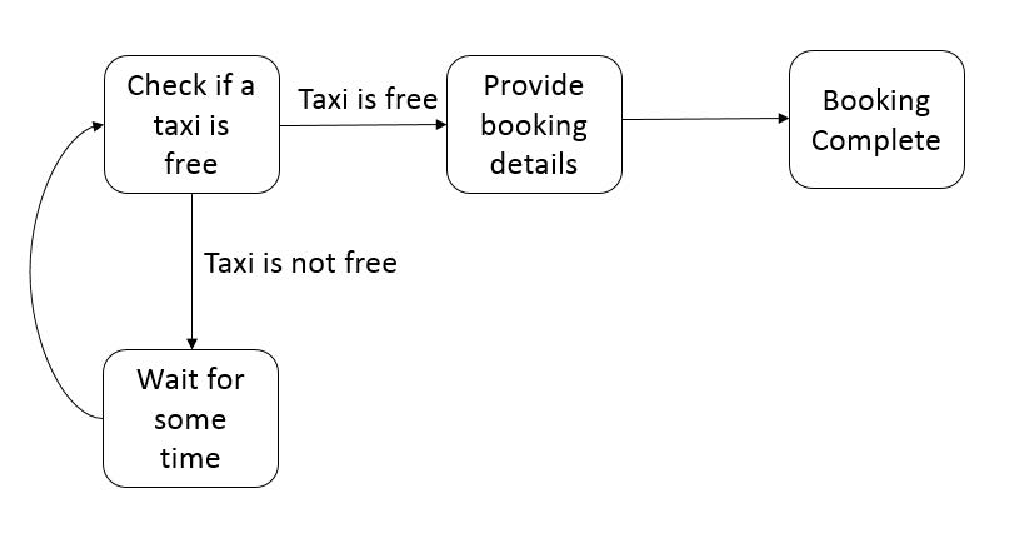
\includegraphics[scale = 0.5]{CPN_abstract_taxi_example.pdf}
	\caption{An abstract model for booking a taxi}
	\label{fig:CPN_abstract_taxi_example}
\end{figure}
\paragraph{\textnormal{Let us consider an example representing a simple online taxi booking service (see Figure \ref{fig:CPN_abstract_taxi_example}). To book a taxi the customer visits the web page. Upon visit, the booking service automatically generates a session identifier. To proceed with the booking process, the system checks for the available taxi. If the taxi is available, then the customer is asked to provide a phone number, pickup time and pickup address. Once the booking information is provided, the booking is finalised and the confirmation is shown to the user. If instead, no taxi is available, the user has to wait until a taxi is free.}}

\section{Coloured Petri Nets (CPNs) Syntax} \label{sec:CPN_Syntax}

\begin{figure}[!htbp]
	\centering
	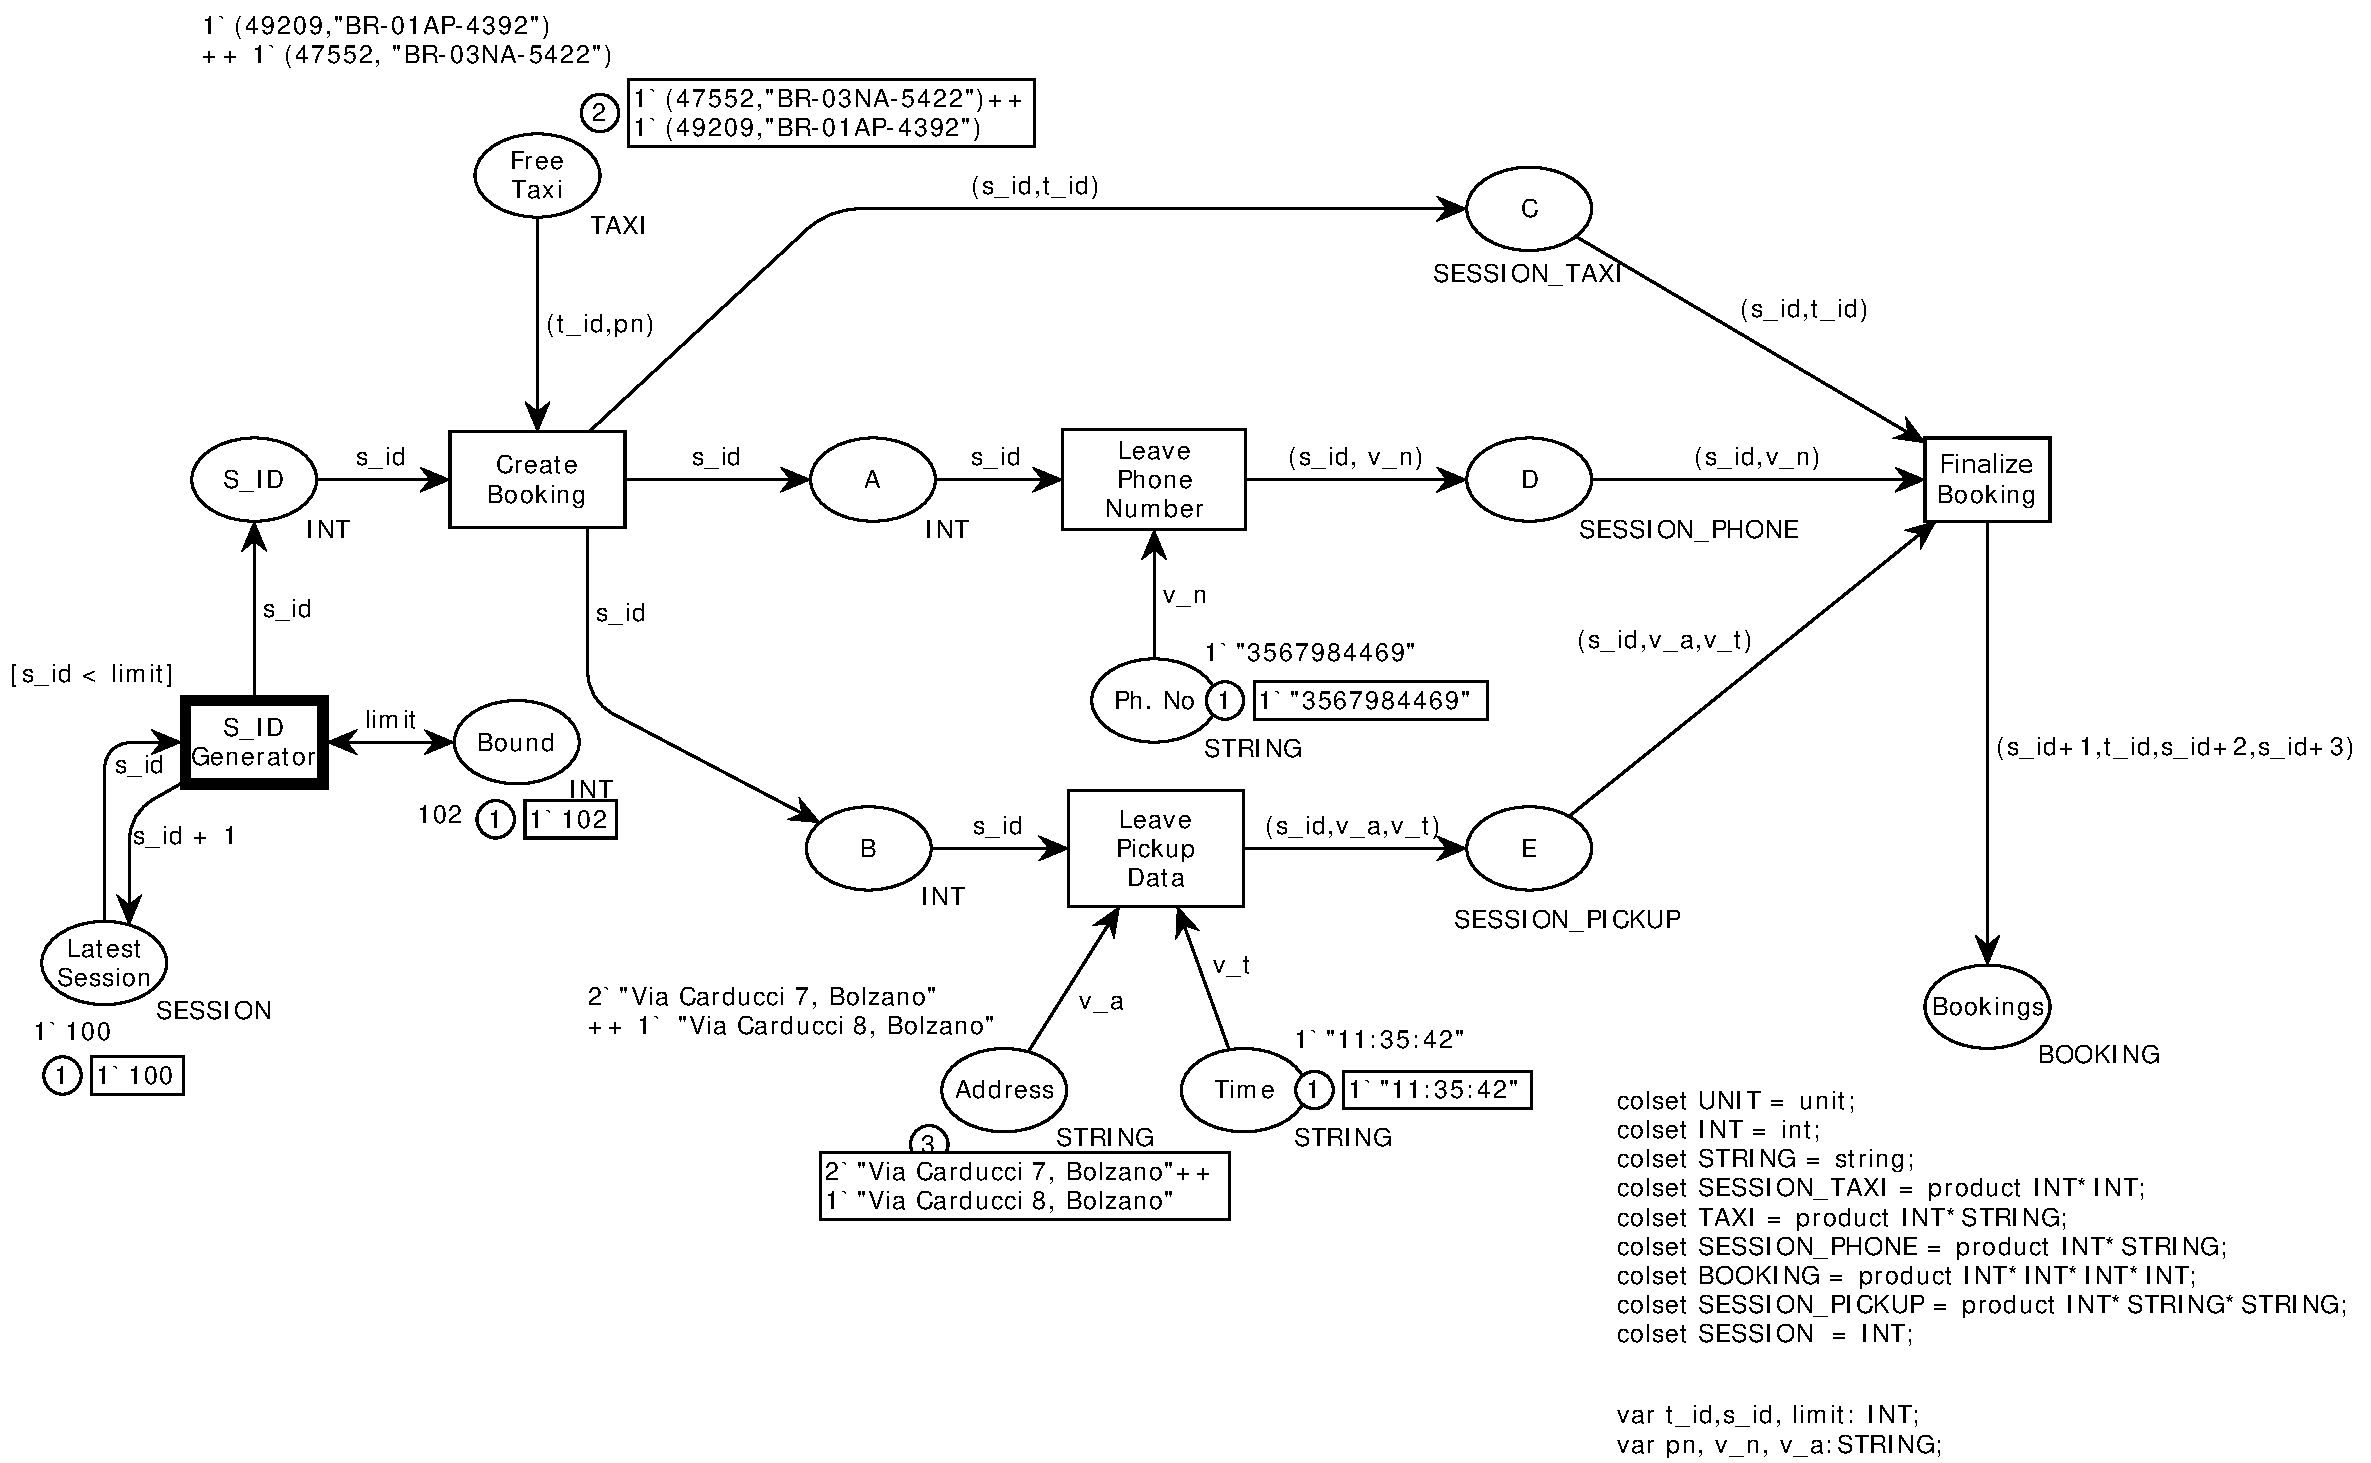
\includegraphics[scale = 0.35]{CPN_Taxi_Booking.pdf}
	\caption{CPN model for taxi booking}
	\label{fig:CPN_Taxi_Booking}
\end{figure}

\subparagraph*{\textnormal{Figure \ref{fig:CPN_Taxi_Booking} shows the CPN model\footnote{This example is modelled in a tool called \bdq{CPN Tools}\cite{CPN_Tools}. CPN Tools uses CPN ML as its programming language.} of the taxi booking example. Here, the places are represented by ellipses and the transitions are represented by rectangles. They are connected to each other by directed arcs. Places represent the state of the system. Each place contains tokens which have data value attached to it. This data value is called \textit{token colour} in CPN. Transitions represent events which can occur in the system. From the classical theory of Petri nets\cite{DBLP:books/daglib/Reisig2013} we know that Petri nets are directed bipartite graph and the bi-partition is between places and transitions, which means that places cannot be connected to places and transitions cannot be connected to transitions.}}

\subparagraph*{\textnormal{A session identifier is generated (at place $\mathit{Latest\ Session}$) incrementally with the starting value as 100. Only 2 session ids can be generated as the guard\footnote{A guard is a boolean expression attached to a transition. In order to make enable a transition, the corresponding guard must evaluate to $\mathit{True}$.} on the $\mathit{S\_ID}$ does not allow to have a session ID greater than the limit which is 102. The transition $\mathit{S\_ID\ Generator}$ is connected to the place $\mathit{Bound}$ with a double headed arc \footnote{It is counted as 2 arcs here, one connecting the place and the transition and the other connecting the same transition and place.}. It does not affect the content of the place. The process proceeds with checking the available taxi and providing the pickup details. $\mathit{Finalize\ Booking}$ transition is called and the confirmed booking is displayed at the place $\mathit{Booking}$. Each booking has a booking id, taxi id, phone id and pickup id. For simplicity and reduced the size of our CPN model, we abstract booking id, taxi id, phone id and pickup id in terms of $\mathit{s\_id}$. We represent them as:
\begin{equation*}
\begin{aligned}
booking\ id = & s\_id + 1\\
phone\ id = & s\_id + 2\\
pickup\ id = & s\_id + 3\\
\end{aligned}
\end{equation*}}}

\subparagraph*{\textnormal{The set of places, transitions, and arcs are denoted by $\mathit{P}$, $\mathit{T}$,and $\mathit{A}$ respectively. In Figure \ref{fig:CPN_Taxi_Booking}, there are 13 places, 5 transitions and 21 directed arcs. The set of places, transitions and arcs are :
\begin{equation*}
\begin{aligned}
P =\ & \{ S\_ID, Free\ Taxi, Address, Time, \ldots \}\footnotemark \\
T =\ &\{ Create\ Booking, Leave\ Phone\ Number, \ldots \} \\
A =\ & \{ (S\_ID, Create\ Booking), (Free\ Taxi, Create Booking),\ldots\}
\end{aligned}
\footnotetext{here in the set notation, \ldots means similarly there are other elements in the set, it should not be confused with an infinite set. The sets are finite.}
\end{equation*}}}

\subparagraph*{\textnormal{In Figure \ref{fig:CPN_Taxi_Booking}, the place $\mathit{Free\ Taxi}$ contains taxis which are not occupied, $\mathit{Bookings}$ contains all the bookings done so far. $\mathit{A}$, $\mathit{B}$, $\mathit{C}$, $\mathit{D}$, $\mathit{E}$ are intermediate places. Places $\mathit{Ph. No}$, $\mathit{Address}$ and $\mathit{Time}$ contain customer's phone number, pickup address and pickup time respectively. For a particular phone number, we have one phone ID which is contained in the place $\mathit{Phone\ ID}$. Similarly, for a booking we have booking id at the place $\mathit{Booking\ ID}$ and for the pickup data, we have a pickup id at place $\mathit{Pickup\ ID}$. The place $\mathit{S\_ID}$ corresponds to session id of a customer. A token is a pair of place and colour-set.}}

\subparagraph*{\textnormal{Each place has a data type attached to it, which is called \textbf{colour-set} of the place. In Figure \ref{fig:CPN_Taxi_Booking}, the colour-set of each place is defined at the bottom right of the place. For example, place $\mathit{S\_ID}$ has the colour-set INT, place $\mathit{Free\ Taxi}$ has the colour-set TAXI. The list of all the colour-set used is provided in Figure \ref{fig:CPN_Taxi_Booking} (in the bottom right corner). In CPN-ML\footnote{CPN Tools uses CPN-ML as its programming language. CPN-ML is an extension of standard ML. Standard ML is a functional programming language, in the sense that the full power of mathematical functions is present. A detailed description of SML is provided in \cite{milner1997definition}. In order to get acquainted with ML programming language in brief and how it used as a programming language with CPN, one can read \cite{Jensen_CPN_Book_ML}.}, the colour-set is written by prefixing the keyword \bdq{COLSET}. The colour-sets STRING and INT are defined as the primitive data type \bdq{string} and \bdq{int} respectively. The colour-set TAXI contains pair (INT, STRING), where the first element represents the taxi id and the second element represents the corresponding plate number.  Similarly, other colour-sets are defined. In general, a colour-set can be cartesian product of different data types.}}

\subparagraph*{\textnormal{We can also restrict the values that a particular colour-set can take. This makes the domain of the colour-set finite\footnote{More information on making finite colour-set is given in \cite{CPN_Tools_ColourSet}}. This is achieved by using the \bdq{with} clause while declaring the colour-set. One such code is provided below. In this code, when we declare the colour-set \bsq{SESSION} we put a limit on the colour-set stating that the value of the integer cannot be less than 100 or greater than 102. Hence by limiting the domain of the colour-set \bsq{SESSION} in the interval $\mathit{\left[100,102\right]}$, we restrict the model to generate a maximum of 2 session ids.}}

\begin{verbatim}
COLSET SESSION = int with 100..102;
\end{verbatim}

\subparagraph*{\textnormal{A \textit{marking} represents the state of the CPN model which is determined by the number of tokens and the token colours on individual places. The marking of a place is determined by the tokens on the specific place. We use the multiset $\mathit{m_{Address}}$ and $\mathit{m_{Free Taxi}}$ to denote the multiset over the colour-set STRING and TAXI respectively corresponding to the markings of the places $\mathit{Address}$ and $\mathit{Free\ Taxi}$ in Figure \ref{fig:CPN_Taxi_Booking}:
\begin{equation*}
\begin{aligned}
&m_{Address} = {2}^{\backprime}\textnormal{"Via Carducci 7, Bolzano"} +\!\!+\ {1}^{\backprime}\textnormal{"Via Carducci 8, Bolzano"}\\
&m_{Free Taxi} = {1}^{\backprime}\textnormal{(49209,\bdsq{(BR-01AP-4392)}} +\!\!+\ {1}^{\backprime}\textnormal{(47552, \bdsq{BR-03NA-5422})}
\end{aligned}
\end{equation*}
This indicates that the place \textit{Address} has the marking which contains 2 tokens of data value \bdsq{Via Carducci 7, Bolzano} and 1 token of data value \bdsq{Via Carducci 8, Bolzano}. The reason for these data values are written in double quotes is because they are of type string. If the number of tokens is 1 then we can omit the number and the ${}^{\backprime}$ operator, and simply write the data value. e.g. ${1}^{\backprime}$\bdsq{Via Carducci 8, Bolzano} can be simply written as \bdsq{Via Carducci 8, Bolzano}. The multiset $m_{Address}$ can be defined as:
\begin{equation*}
m_{Address}(s) = \begin{cases}
2 & \textit{if s = \textnormal{\bdsq{Via Carducci 7, Bolzano}}} \\ 
1 & \textit{if s = \textnormal{\bdsq{Via Carducci 8, Bolzano}}} \\ 
0 & \textit{otherwise}
\end{cases}
\end{equation*}
Similarly, for the place $\mathit{Free\ Taxi}$, one could write it as:
\begin{equation*}
m_{Free Taxi}(s) = \begin{cases}
1 & \textit{if s = \textnormal{(49209,\bdsq{BR-01AP-4392})}} \\ 
1 & \textit{if s = \textnormal{(47552,\bdsq{BR-03NA-5422})}} \\ 
0 & \textit{otherwise} 
\end{cases}
\end{equation*}}}
\begin{comment}
Where the ${}^{\backprime}$ is the infix operator, the number preceding the symbol ${}^{\backprime}$ signifies the number of tokens while the tuple succeeding the symbol represents the data value.	content...
\end{comment}

\subparagraph*{\textnormal{Let us now formally define elements that constitute \textbf{net inscriptions}, i.e., arc expressions, guards and colour-sets. Arc expressions are the expressions written on the arcs. We denote by $\mathit{EXPR}$ the set of expressions provided by the inscription language. Here, the inscription language is a general term for a backend language used to specify colour-sets and operations over them. However, in our case, we rely on a specific language, i.e., CPN ML provided by CPNTools. Given an expression $\mathit{e \in EXPR}$, the \textbf{\textit{type}} of $\mathit{e}$, represented by $\mathit{Type[e]}$, specifies the colour of values obtained by evaluating $\mathit{e}$. The set of \textbf{\textit{free variables}} in an expression $\mathit{e}$ is denoted by $\mathit{Var[e]}$, and the type of a variable $\mathit{v}$ is denoted by $\mathit{Type[v]}$. $\mathit{V}$ denotes the set of variables. Note that a free variable is a variable which is not bound in the local environment of the expression.
In Figure \ref{fig:CPN_Taxi_Booking}, for the arc expressions we have the following free variables:
\begin{equation*}
\mathit{Var[e]} = \begin{cases}
\mathit{\{s\_id\}} & \textit{if e = s\_id}\\ 
\mathit{\{t\_id, pn\}} & \textit{if e = \textnormal{(}t\_id, pn\textnormal{)}} \\ 
\mathit{\{s\_id, t\_id\}} & \textit{if e = \textnormal{(}s\_id, t\_id\textnormal{)}} \\ 
\mathit{\{v\_n\}} & \textit{if e = \textnormal{(}v\_n\textnormal{)}}\\ 
\ldots
\end{cases}
\end{equation*}}}
\subparagraph*{\textnormal{$\mathit{\Sigma}$ denotes the set of \textbf{\textit{colour-sets}} defined for the CPN model. Given a set of variables $\mathit{V}$, for all $\mathit{v \in V : Type[v] \in \Sigma}$. For $\mathit{V' \subseteq V}$, the set of expressions $\mathit{e \in EXPR}$ such that $\mathit{Var[e] \subseteq V'}$ is denoted $\mathit{EXPR_{V'}}$. For the CPN model in Figure \ref{fig:CPN_Taxi_Booking}, the colour-sets are defined as:
\begin{equation*}
\begin{aligned}
\mathit{\Sigma = \{ INT, STRING, TAXI, SESSION\_TAXI, \ldots \}}
\end{aligned}
\end{equation*}
We define the set of free variables in our CPN model:
\begin{equation*}
\begin{aligned}
\mathit{V = \{s\_id : INT, t\_id : INT, v\_a : STRING, v\_t : STRING, \ldots\}}
\end{aligned}
\end{equation*}}}

\subparagraph*{\textnormal{The \textbf{\textit{colour-set function}} is a function, $\mathit{C : P \rightarrow \Sigma}$, which maps every place to its corresponding colour-set. The colour-set function for the CPN model in Figure \ref{fig:CPN_Taxi_Booking} is:}}

\begin{equation*}
C(p) = \begin{cases}
\mathit{INT} & \textit{if p $\in$ \textnormal{\{}S\_ID, A, B, Bound\textnormal{\}}}\\
\mathit{STRING} & \textit{if p $\in$ \textnormal{\{}Ph. No, Address, Time\textnormal{\}}}\\
\mathit{TAXI} & \textit{if p = Free Taxi}\\
\mathit{SESSION\_TAXI} & \textit{if p = C}\\
\mathit{SESSION\_PHONE} & \textit{if p = D}\\
\mathit{SESSION\_PICKUP} & \textit{if p = E}\\
\mathit{BOOKING} & \textit{if p = Bookings} \\
\mathit{SESSION} & \textit{if p = Latest Session}
\end{cases}
\end{equation*}
\paragraph*{\textnormal{\textit{Guard} is a boolean expression attached to the transitions. For a transition be enabled it is a necessary condition that the guard of the transition should evaluate to $\mathit{True}$. A function $\mathit{G : T \rightarrow EXPR_{V}}$ is called a \textbf{\textit{guard function}} and assigns every transition $\mathit{t \in T}$ a boolean expression, i.e., $\mathit{Type[G(t)] = Bool}$. The set of free variables occurring in a guard should be a subset of $\mathit{V}$, hence, $\mathit{G(t) \in EXPR_{V}}$. The CPN model, in Figure \ref{fig:CPN_Taxi_Booking}, has guard function defined as:
}}

\begin{equation*}
G(t) = \begin{cases}
\mathit{s\_id < limit} & $\textit{if t = S\_ID Generator}$\\
\mathit{True} & $\textit{otherwise}$
\end{cases}
\end{equation*}

\subparagraph*{\textnormal{A function $E : A \rightarrow EXPR_{V}$ is called \textbf{\textit{arc expression function}} which assigns every $a \in A$ an expression $E(a)$. Similar to the guards of the transition, the free variables occurring in $E(a)$ has to be a subset of $V$, hence, $E(a) \in EXPR_{V}$. For an arc $(p,t) \in A$, connecting a place $p \in P$ and a transition $t \in T$, it is required that the type of the arc expression is the multiset type over the colour-set $C(p)$ of the place $p$, i.e., $Type[E(p, t)] = C(p)_{MS}$. This is for the directed arc from a place to a transition. Similarly it can be applied to a directed arc from a transition to a place. For an arc $(t,p) \in A$ it is required that $Type[E(t, p)] = C(p)_{MS}$. For the model in Figure \ref{fig:CPN_Taxi_Booking}, the arc expression function is defined as:}}
\begin{equation*}
E(a) = \begin{cases}
{1}^{\backprime}(s\_id) & \textit{if a $\in$ \textnormal{\{(}S\_ID, Create Booking\textnormal{)},}\\
& \textit{\textnormal{(}Create Booking, A\textnormal{)},\textnormal{(}Create Booking, B\textnormal{)},}\\
& \textit{\textnormal{(}A, Leave Phone Number\textnormal{)},}\\ 
& \textit{\textnormal{(}B, Leave Pickup Data\textnormal{)\}}}\\
{1}^{\backprime}(s\_id,t\_id) & \textit{if a $\in$ \textnormal{\{(}Create Booking, C\textnormal{)},}\\ 
& \textit{\textnormal{(}E, Finalize Booking\textnormal{)\}}}\\
{1}^{\backprime}(v\_n) & \textit{if a = \textnormal{(}Ph. No, Leave Phone Number\textnormal{)}}\\
\ldots
\end{cases}
\end{equation*}

\subparagraph*{\textnormal{The initialization function gives initial marking to all places in the model. The \textbf{\textit{initialization function}} $\mathit{I : P \rightarrow EXPR_{0}}$ assigns to each place $\mathit{p}$ an initialization expression $\mathit{I(p)}$ which is required to evaluate to a multiset over the colour-set of the place $\mathit{p}$, i.e., $\mathit{Type[I(p)] = C(p)_{MS}}$. The initialization expression must be a closed expression, i.e., it cannot have any free variables, hence $\mathit{I(p) \in EXPR_{\emptyset}}$. A possible initialization function for the model in Figure \ref{fig:CPN_Taxi_Booking} is given by:
\begin{equation*}
I(p) = \begin{cases}
\textnormal{${1}^{\backprime}$(49209,\bdsq{BR-01AP-4392})} +\!\!+  & \textit{if p = Free Taxi}\\
\textnormal{${1}^{\backprime}$(47552,\bdsq{BR-03NA-5422})} & \\
\textnormal{${2}^{\backprime}$\bdsq{Via Carducci 7, Bolzano}} +\!\!+ & \textit{if p = Address}\\ 
\textnormal{${1}^{\backprime}$\bdsq{Via Carducci 8, Bolzano}} & \\
\textnormal{${1}^{\backprime}$\bdsq{11:35:42}} & \textit{if p = Time}\\
\textnormal{${1}^{\backprime}$\bdsq{3567984469}} & \textit{if p = Ph. No}\\
\textnormal{${1}^{\backprime}$100} & \textit{if p = Latest Session}\\
\textnormal{${1}^{\backprime}$102} & \textit{if p = Bound}\\
\emptyset_{MS} & \textit{otherwise}
\end{cases}
\end{equation*}}}

\subparagraph*{\textnormal{With the explanation of the above functions, we  define non-hierarchical coloured petri nets.}}

\begin{defs}
	\label{defs:CPN_NonHeir}
	A non-hierarchical Coloured Petri Net is a tuple $\mathit{CPN} = \mathit{(P,T,A,\Sigma,V,C,G,E,I)}$, where:
	\begin{itemize}
		\item $\mathit{P}$ is a finite set of places.
		\item $\mathit{T}$ is a finite set of transitions $\mathit{T}$ such that $\mathit{P \cap T = \emptyset}$.
		\item $\mathit{A \subseteq (P \times T) \cup (T \times P)}$ is a set of directed arcs.
		\item $\mathit{\Sigma}$ is a finite set of non-empty colour-sets.
		\item $\mathit{V}$ is a finite set of typed variables such that $\mathit{Type[v] \in \Sigma}$ for all variables $\mathit{v \in V}$.
		\item $\mathit{C : P \rightarrow \Sigma}$ is a colour-set function that assigns a colour-set to each place.
		\item $\mathit{G : T \rightarrow EXPR_{V}}$ is a guard function that assigns a guard to each transition $\mathit{t}$ such that $\mathit{Type[G(t)] = Bool}$.
		\item $\mathit{E : A \rightarrow EXPR_{V}}$ is an arc expression function that assigns an arc expression to each arc $\mathit{a}$ such that $\mathit{Type[E(a)] = C(p)_{MS}}$, where $\mathit{p}$ is the place connected to the arc $\mathit{a}$.
		\item $\mathit{I : P \rightarrow EXPR_{\emptyset}}$ is an initialization function that assigns an initialization expression to each place $\mathit{p}$ such that $\mathit{Type[I(p)] =C(p)_{MS}}$.
	\end{itemize}
\end{defs}

\section{Colored Petri Nets (CPNs) Semantics} \label{sec:CPN_Semantics}
\paragraph{\textnormal{In this section, we discuss about markings and binding elements. Later, we look at a step, enabling and occurrence of steps and when a step occurs how it effects the marking of the net. We also discuss the conditions when the transition is enabled. In the end, we discuss reachable markings and state spaces.}}
\subsection*{Enabling and Occurrence of Steps}

\begin{comment}
\paragraph{\textnormal{In this section, we discuss about markings and binding elements. Later, we look at a step, enabling and occurrence of steps and when a step occurs how it effects the marking of the net. We also discuss the conditions when the transition is enabled. In the end, we discuss reachable markings and state spaces.}}
\end{comment}

\subparagraph{\textnormal{In a given marking, the enabling rule specifies when a step (consisting of a multiset of binding elements) becomes enabled, whereas the firing/occurrence rule specifies how the markings change when the enabled step occurs.}}

\begin{figure}[!htbp]
	\centering
	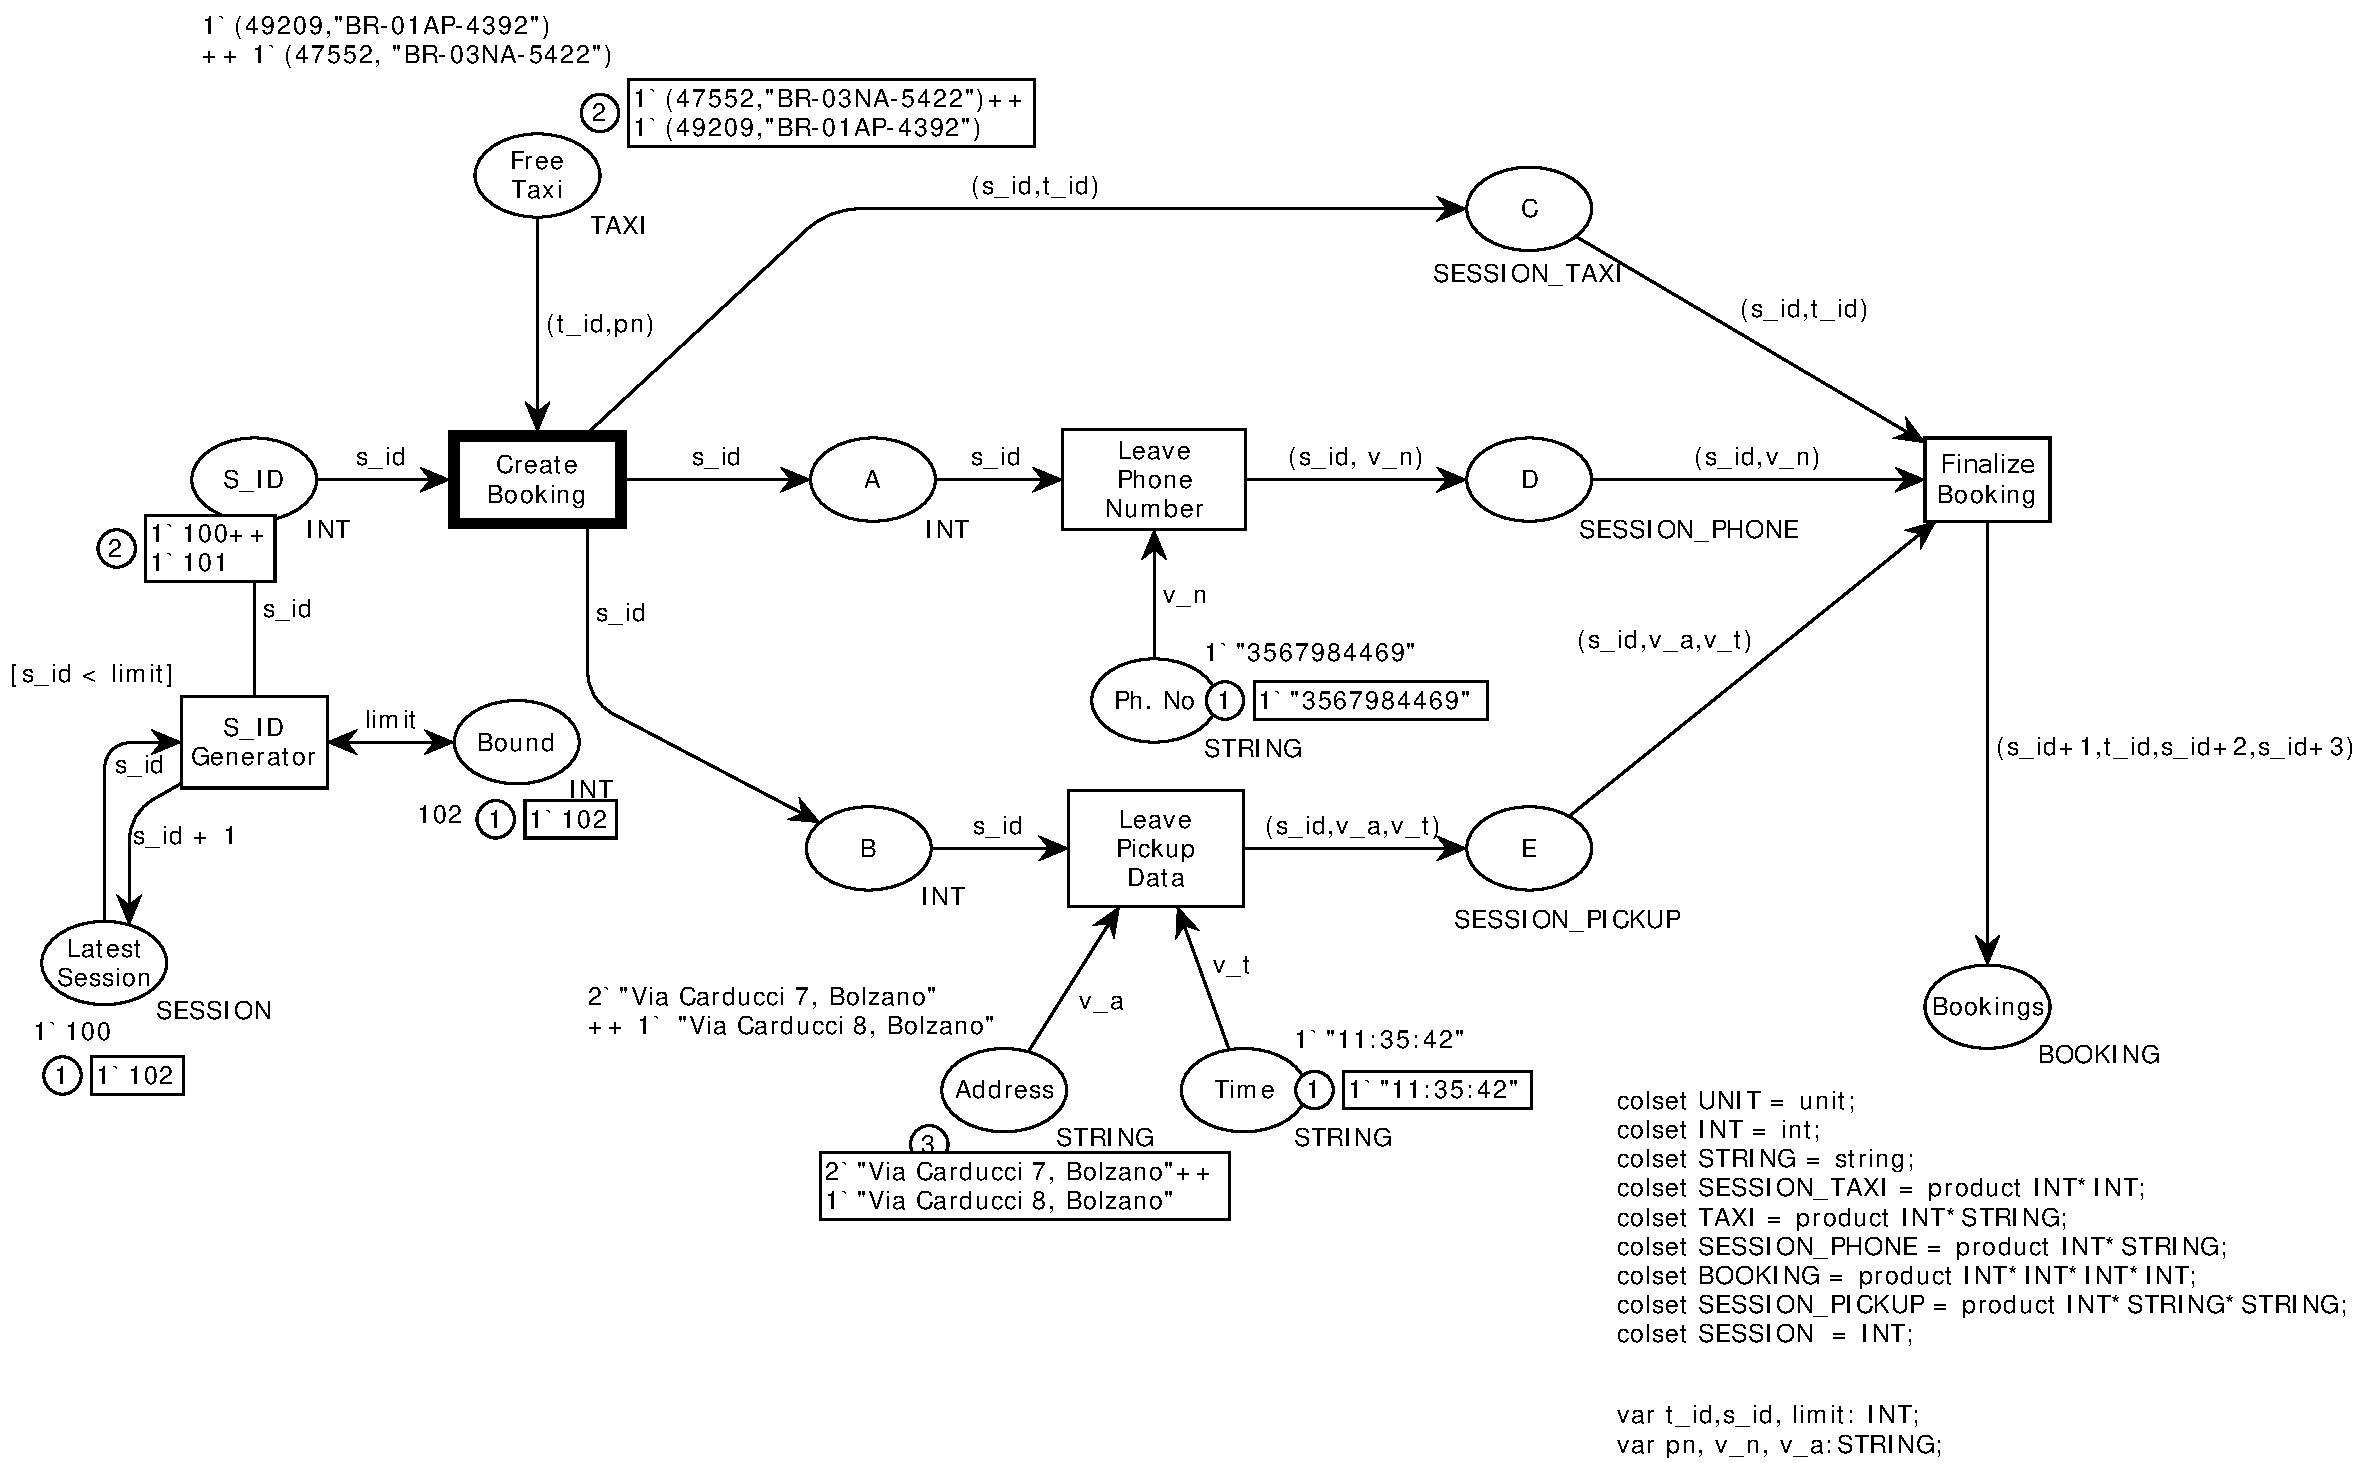
\includegraphics[scale = 0.35]{CPN_Taxi_Booking_initial_step.pdf}
	\caption{CPN model for taxi booking}
	\label{fig:CPN_Taxi_Booking_initial_step}
\end{figure}

\subparagraph*{\textnormal{A \textbf{\textit{marking}} $\mathit{M}$ is a function that maps each place $\mathit{p}$ into a multiset of values $\mathit{M(p)}$ representing the marking of $\mathit{p}$. The individual elements in the multiset $\mathit{M(p)}$ are called \textbf{\textit{tokens}}. The multiset of tokens present on a place $\mathit{p}$ in a marking $\mathit{M}$ is required to match the type of the place, i.e., $\mathit{M(p) \in C(p)_{MS}}$. For example, the marking of the places for the CPN model presented in Figure \ref{fig:CPN_Taxi_Booking_initial_step} is given by\footnote{The markings in the model are represented by rectangles beside each place.}:}}

\begin{equation*}
M(p) = \begin{cases}
{1}^{\backprime}100 +\!\!+ {1}^{\backprime}101 & \textit{if p = S\_ID}\\
\textnormal{${1}^{\backprime}$(49209,\bdsq{BR-01AP-4392})} +\!\!+  & \textit{if p = Free Taxi}\\
\textnormal{${1}^{\backprime}$(47552,\bdsq{BR-03NA-5422})} & \\
\textnormal{${2}^{\backprime}$\bdsq{Via Carducci 7, Bolzano}} +\!\!+ & \textit{if p = Address}\\ 
\textnormal{${1}^{\backprime}$\bdsq{Via Carducci 8, Bolzano}} & \\
\textnormal{${1}^{\backprime}$\bdsq{11:35:42}} & \textit{if p = Time}\\
\textnormal{${1}^{\backprime}$\bdsq{3567984469}} & \textit{if p = Ph. No}\\
\textnormal{${1}^{\backprime}$102} & \textit{if p = Latest Session}\\
\textnormal{${1}^{\backprime}$102} & \textit{if p = Bound}\\
\emptyset_{MS} & \textit{otherwise}
\end{cases}
\end{equation*}

\subparagraph*{\textnormal{$\mathit{Var(t)}$ denotes \textbf{\textit{variables of a transition}} $\mathit{t}$, which consists of free variables appearing either in any of the arc expression connecting the transition or in the guard of the transition. The variables for the transitions for the model in the Figure \ref{fig:CPN_Taxi_Booking_initial_step} are:}}
\begin{equation*}
Var(t) = \begin{cases}
\{s\_id,t\_id,pn\} & \textit{if t = Create Booking}\\
\{s\_id,v\_n\} & \textit{if t = Leave Phone Number}\\
\{s\_id,v\_a,v\_t\} & \textit{if t = Leave Pickup Data}\\
\{s\_id,t\_id,v\_n,v\_a,v\_t\} & \textit{if t = Finalize Booking}\\
\{s\_id,limit\} & \textit{if t = S\_ID Generator} 
\end{cases}
\end{equation*}

\subparagraph*{\textnormal{The \textbf{\textit{initial marking}}, denoted by $\mathit{M_{0}}$, is obtained by evaluating the initialization expression. The initialization expression does not contain any free variables and its evaluation is with the empty binding (denoted by $\mathit{\langle \rangle}$), i.e., $\mathit{M_{0}(p) = I(p)\langle \rangle,}$ for each $\mathit{p \in P}$. The initial marking for this example (Figure \ref{fig:CPN_Taxi_Booking}) is given by:}}

\begin{equation*}
M_{0}(p) = \begin{cases}
\textnormal{${1}^{\backprime}$(49209,\bdsq{BR-01AP-4392})} +\!\!+  & \textit{if p = Free Taxi}\\
\textnormal{${1}^{\backprime}$(47552,\bdsq{BR-03NA-5422})} & \\
\textnormal{${2}^{\backprime}$\bdsq{Via Carducci 7, Bolzano}} +\!\!+ & \textit{if p = Address}\\ 
\textnormal{${1}^{\backprime}$\bdsq{Via Carducci 8, Bolzano}} & \\
\textnormal{${1}^{\backprime}$\bdsq{11:35:42}} & \textit{if p = Time}\\
\textnormal{${1}^{\backprime}$\bdsq{3567984469}} & \textit{if p = Ph. No}\\
\textnormal{${1}^{\backprime}$100} & \textit{if p = Latest Session}\\
\textnormal{${1}^{\backprime}$102} & \textit{if p = Bound}\\
\emptyset_{MS} & \textit{otherwise}
\end{cases}
\end{equation*}

\subparagraph*{\textnormal{A \textbf{\textit{binding}} $b$ of a transition $t$ is a function that maps each variable $v$ of the transition $t$ to a value $b(v)$ belonging to the type of the variable $v$, i.e., $b(v) \in Type[v]$. Bindings are written as $\langle var_{1} = val_{1},var_{2} = val_{2}, \ldots ,var_{n} = val_{n} \rangle$, where $var_{1}, var_{2}, \ldots , var_{n}$ are the variables in $Var(t)$ and $val_{i}$ is the value bound to the variable $var_{i}$. A \textbf{\textit{binding element}} is a pair $(t,b)$ consisting of a transition $t$ and a binding $b$ of $t$. A step is a non-empty, finite multiset of binding elements.}}

\subparagraph*{\textnormal{With the above functions at hand, we define few concepts related to CPN.}}

\begin{defs}
	\label{defs:2_7_step_marking}
	For a Coloured Petri Net $\mathit{CPN = (P,T,A,\Sigma,V,C,G,E,I)}$:
	\begin{enumerate}
		\item A \textbf{marking} is a function $\mathit{M}$ that maps each place $\mathit{p \in P}$ into a multiset of tokens
		$\mathit{M(p) \in C(p)_{MS}}$.
		\item The \textbf{initial marking} $\mathit{M_{0}}$ is defined by $\mathit{M_{0}(p) = I(p)}$ for all $\mathit{p \in P}$.
		\item The \textbf{variables of a transition} $\mathit{t}$ are denoted $\mathit{Var(t) \subseteq V}$ and consist of the free variables appearing in the guard of $\mathit{t}$ and in the arc expressions of arcs connected to $\mathit{t}$.
		\item A \textbf{binding} of a transition $\mathit{t}$ is a function $\mathit{b}$ that maps each variable $\mathit{v \in Var(t)}$ into a value $\mathit{b(v) \in Type[v]}$. The set of all bindings for a transition $\mathit{t}$ is denoted $\mathit{B(t)}$.
		\item A \textbf{binding element} is a pair $\mathit{(t,b)}$ such that $\mathit{t \in T}$ and $\mathit{b \in B(t)}$. The set of all binding elements $\mathit{BE(t)}$ for a transition $\mathit{t}$ is defined by $\mathit{BE(t)} = \mathit{\{(t,b) | b \in B(t)\}}$. The set of all binding elements in a CPN model is denoted $\mathit{BE}$.
		\item A \textbf{step} $\mathit{Y \in BE_{MS}}$ is a non-empty, finite multiset of binding elements.
	\end{enumerate}
\end{defs}

\subparagraph*{\textnormal{As stated earlier, the transitions have guards attached to them and the arcs carry expressions with them (arc expressions). These two determine the enabling and occurrence of a step. For a binding element $\mathit{(t,b)}$ where $\mathit{t}$ is a transition and $\mathit{b}$ is a binding, the guard expression $\mathit{G(t)}$ of the transition is evaluated against the binding $\mathit{b}$ and the result is written as $\mathit{G(t)\langle b \rangle}$. Similarly, the arc expression $\mathit{E(a)}$ (for any arc $\mathit{a}$) is also evaluated against the binding $\mathit{b}$ and the result is written as $\mathit{E(a)\langle b \rangle}$. For an arc $\mathit{a = (p,t)}$, which connects a place $\mathit{p}$ and a transition $\mathit{t}$, the arc expression $\mathit{E(p,t)}$ denotes the arc expression on the input arc from $\mathit{p}$ to $\mathit{t}$. When no such arc exists, we define $\mathit{E(p, t) = \emptyset_{MS}}$. Analogously, $\mathit{E(t, p)}$ denotes the arc expression on the output arc from $\mathit{t}$ to $\mathit{p}$. When no such arc exists, we define $\mathit{E(t, p) = \emptyset_{MS}}$.}}

\subparagraph*{\textnormal{For a binding $\mathit{(t,b)}$ to be enabled in a making $M$ there are two conditions to satisfy:
\begin{itemize}
\item The evaluation of the guard expression - In order for a binding to get enabled, the corresponding guard expression must evaluate to $\mathit{True}$.
\item The number of tokens in the input place - for each place $\mathit{p}$, an arc expression $\mathit{E(p,t)}$ has to be evaluated to the binding $\mathit{b}$ such that $\mathit{E(p,t)\langle b \rangle\ll=M(P)}$. It means that for each place $\mathit{p}$ there should be enough tokens that transition $\mathit{t}$ will remove when occurring with binding $\mathit{b}$.
\end{itemize}
}}

\subparagraph*{\textnormal{Let us look at the two conditions in our taxi booking example. Since we do not have any guards on our model the guard function evaluates to $\mathit{True}$ for all transitions in the model. Let us consider a binding element $\mathit{(Create\ Booking, b_{CB})}$ where
\begin{equation}
\label{eq:binding_1}
b_{CB} = \langle s_{id} = 100, t_{id} = 47552, pn = \textnormal{"BR-03NA-5422"}\rangle
\end{equation}
Alternatively, $b_{CB}$ can also be chosen as:
\begin{equation}
\label{eq:binding_2}
b_{CB} = \langle s_{id} = 101, t_{id} = 49209, pn = \textnormal{"BR-01AP-4392"}\rangle
\end{equation}
One of the important properties of CPN is non-determinism. Here, the values for the binding $\mathit{b_{CB}}$ can be chosen non-deterministically. Here, we will select the binding given in equation \ref{eq:binding_1}. From the input arcs of the $\mathit{Create\ Booking}$ transition, we have
\begin{equation*}
\begin{aligned}
E(S\_ID, Create\ Booking)\langle b_{CB}\rangle =& {1}^{\backprime}100 \ll = {1}^{\backprime}100\ +\!\!+\ {1}^{\backprime}101\\
E(Free\ Taxi, Create\ Booking)\langle b_{CB}\rangle =& {1}^{\backprime}(47552,\textnormal{"BR-03NA-5422"})\\ 
& \ll = {1}^{\backprime}(49209,\textnormal{"BR-01AP-4392"}) +\!\!+\ \\
& {1}^{\backprime}(47552,\textnormal{"BR-03NA-5422"})
\end{aligned}
\end{equation*}}}

\subparagraph*{\textnormal{When an enabled binding $\mathit{(t,b)}$ occurs \footnote{The thick border around the transition (see Figure \ref{fig:CPN_Taxi_Booking_initial_step}) signifies that the transition is enabled.}, the tokens are consumed from the input place and produced at the output place. The amount of tokens consumed or produced depends on the arc inscription attached to the respective arcs. The multiset of tokens removed from the input place $\mathit{p}$, when $\mathit{t}$ occurs in $\mathit{b}$ is given by $\mathit{E(p,t)\langle b \rangle}$, and the multiset of tokens added to an output place $\mathit{p}$ is given by: $\mathit{E(t,p)\langle b \rangle}$, which means that the new marking $\mathit{M'}$ reached when an enabled binding element $\mathit{(t,b)}$ occurs in a marking $\mathit{M}$ is given by:
\begin{equation*}
M'(p) = (M(p) -\!-\ E(p, t)\langle b \rangle) +\!\!+\ E(t, p)\langle b \rangle , \forall p \in P
\end{equation*}}}

\subparagraph*{\textnormal{For our model in Figure \ref{fig:CPN_Taxi_Booking}, let us calculate the new marking $M^{'}$ assuming the binding element (\textit{Create Booking, $b_{CB}$}) occurs.}}
\begin{equation*}
\begin{aligned}
M^{'}(S\_ID) =\ & ({1}^{\backprime}100\ +\!\!+\ {1}^{\backprime}101 -\!- \ {1}^{\backprime}100) +\!\!+\ \emptyset_{MS}\\
=\ & {1}^{\backprime}101 \\
M^{'}(Free\ Taxi) =\ & ({1}^{\backprime}(49209,\textnormal{"BR-01AP-4392"}) +\!\!+\ {1}^{\backprime}(47552,\textnormal{"BR-03NA-5422"})\\  
& -\!-\ {1}^{\backprime}(47552,\textnormal{"BR-03NA-5422"})) +\!\!+\ \emptyset_{MS}\\ 
=\ & {1}^{\backprime}(49209,\textnormal{"BR-01AP-4392"})\\ 
M^{'}(A) =\ &(\emptyset_{MS} -\!-\ \emptyset_{MS}) +\!\!+\ {1}^{\backprime}100 \\
=\ &{1}^{\backprime}100\\
M^{'}(B) =\ &(\emptyset_{MS} -\!-\ \emptyset_{MS}) +\!\!+\ {1}^{\backprime}100 \\
=\ &{1}^{\backprime}100\\
M^{'}(C) =\ &(\emptyset_{MS} -\!-\ \emptyset_{MS}) +\!\!+\ {1}^{\backprime}(100,47552)\\
=\ &{1}^{\backprime}(100,47552)
\end{aligned}
\end{equation*}

\begin{figure}[!htbp]
	\centering
	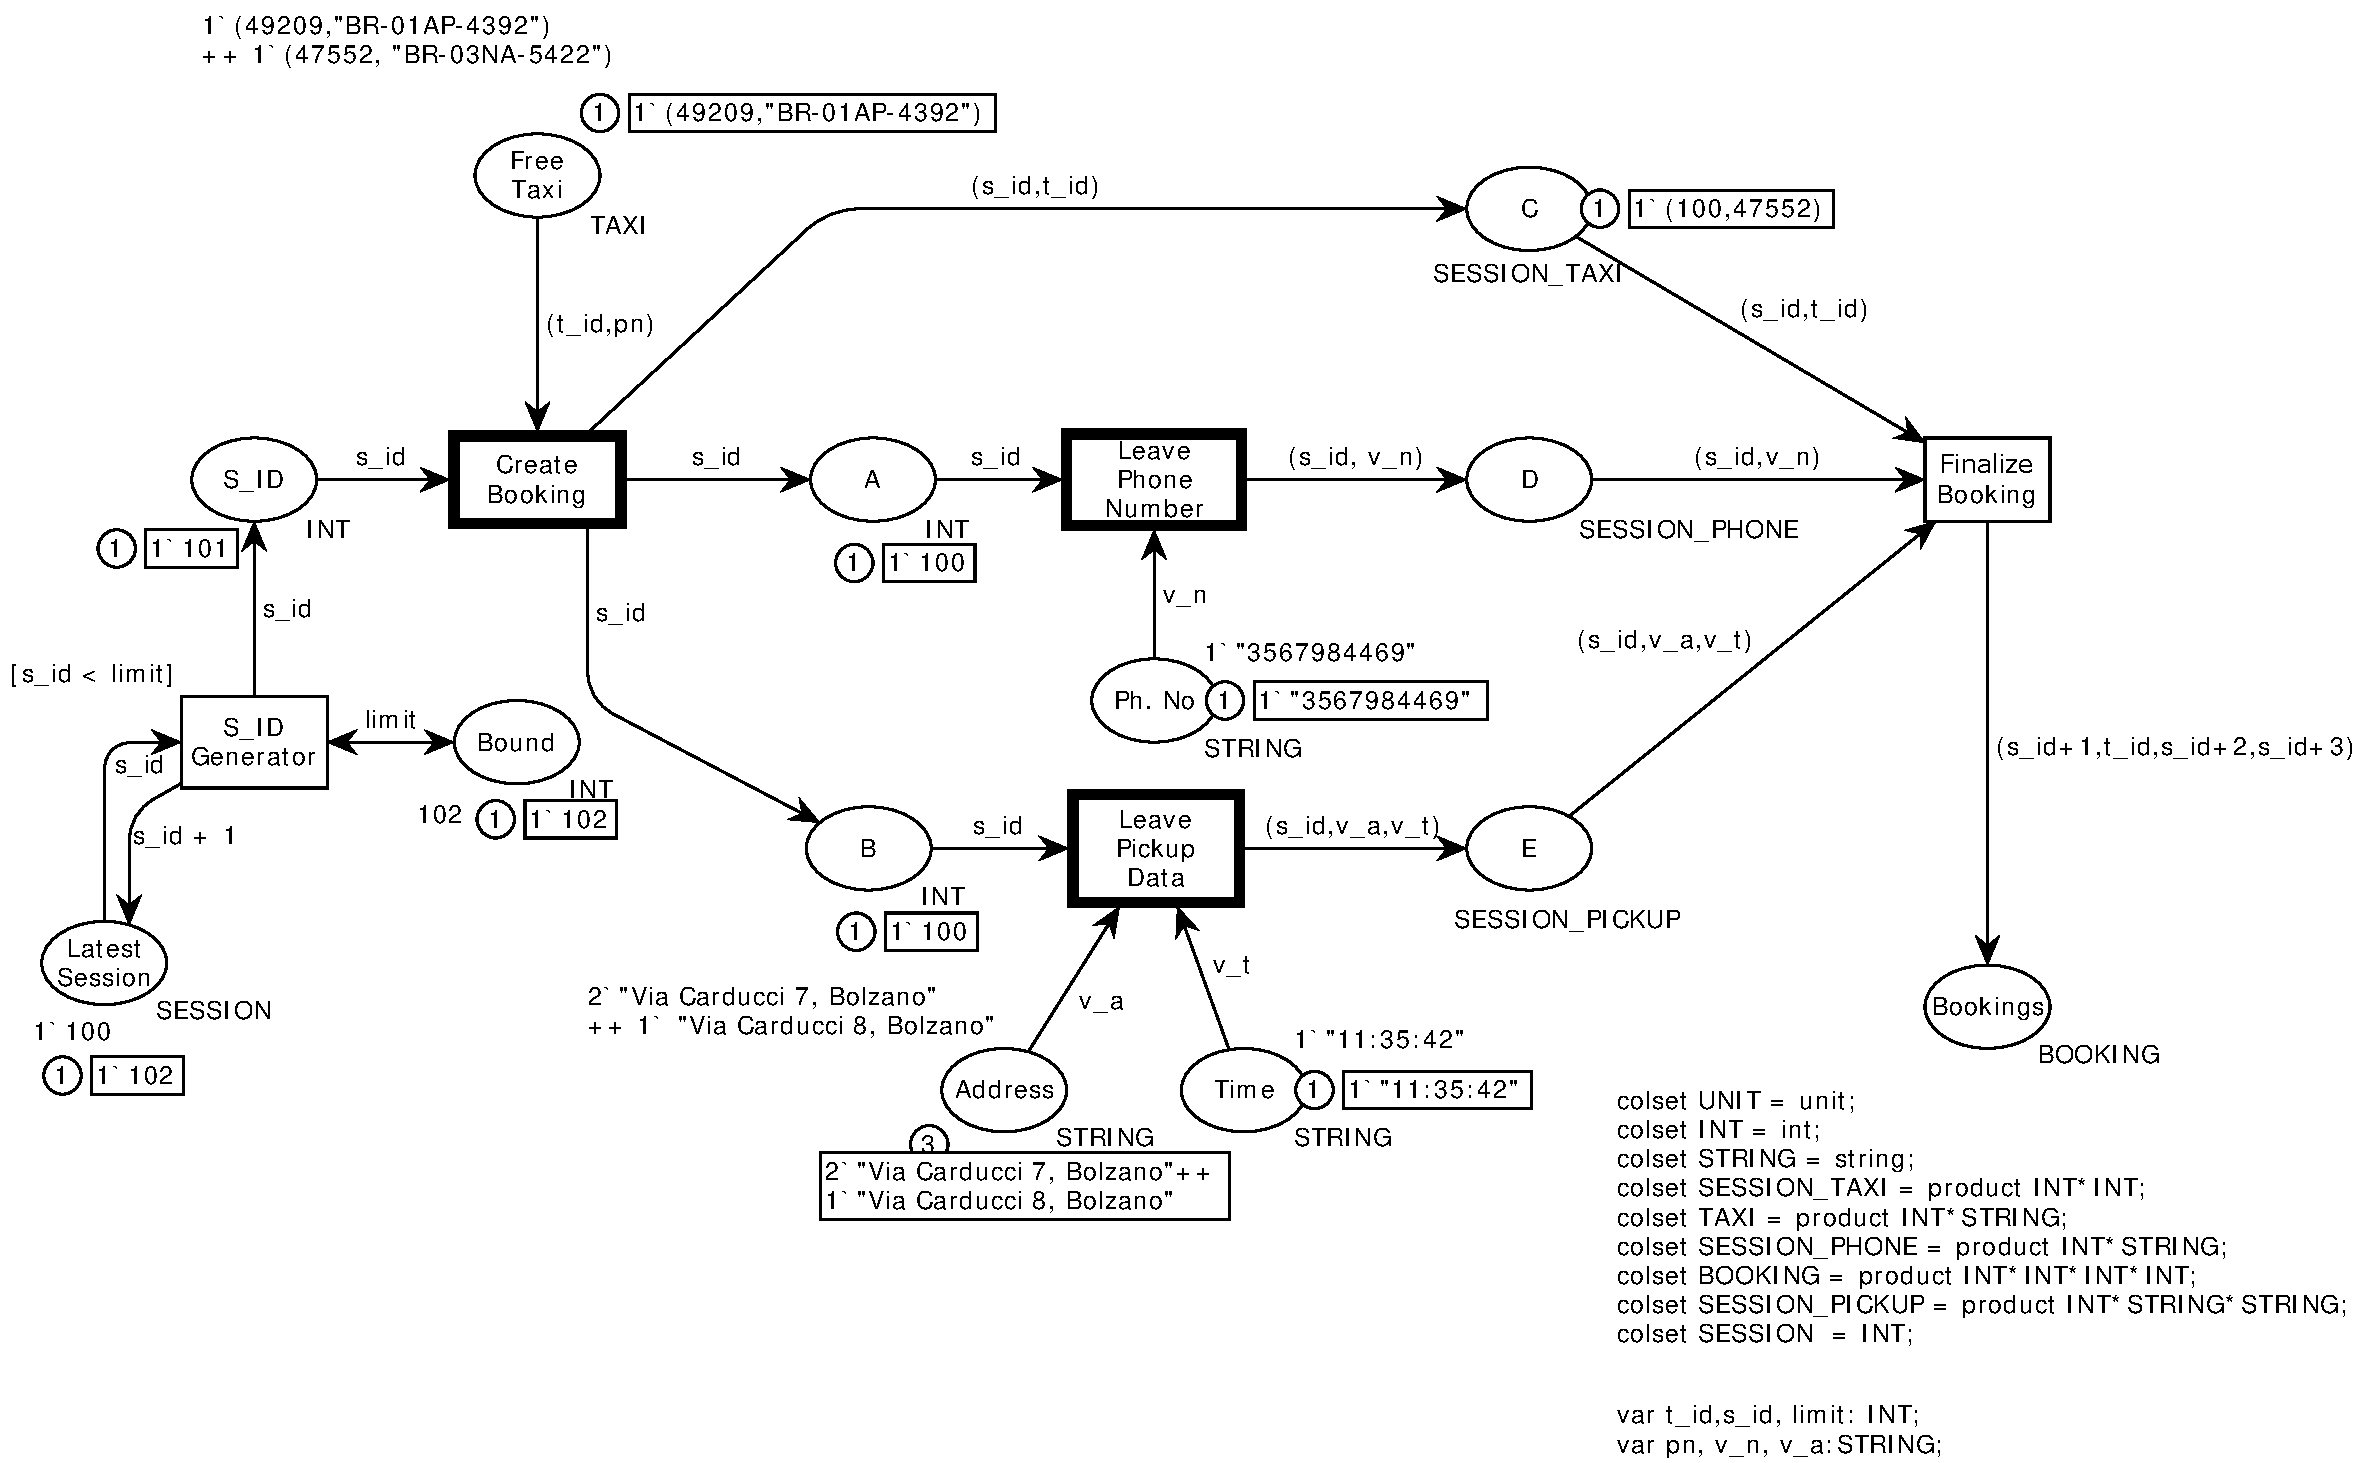
\includegraphics[scale = 0.35]{CPN_Taxi_Booking_one_step.pdf}
	\caption{A state of the CPN model for taxi booking}
	\label{fig:CPN_Taxi_Booking_one_step}
\end{figure}

\subparagraph*{\textnormal{In Figure \ref{fig:CPN_Taxi_Booking_one_step}, there are 3 transitions which are enabled, namely, $\mathit{Create\ Booking}$, $\mathit{Leave\ Phone\ Number}$ and $\mathit{Leave\ Pickup\ Data}$. This is the synchronization property of CPNs where there are multiple transitions enabled and each such transition may fire. The simulation(execution of transitions) is halted when there are no more enabled transitions.}}

\subparagraph*{\textnormal{Now with the explanation of how we can determine enabling and occurrence of steps, let us visit the definition of enabling and occurrence of a binding element in a coloured Petri net.}}
\begin{defs}
	\label{defs:enabling_binding_cpn}
	A binding element $\mathit{(t,b) \in BE}$ is \textbf{enabled} in a marking $\mathit{M}$ if and only
	if the following two properties are satisfied:
	\begin{enumerate}
		\item $\mathit{G(t)\langle b \rangle}$.
		\item $\mathit{\forall p \in P : E(p,t)\langle b \rangle \ll= M(p)}$.
		\item When $\mathit{(t,b)}$ is enabled in $\mathit{M}$, it may \textbf{occur}, leading to the marking $\mathit{M}$ defined by:
		\begin{equation*}
			\forall p \in P : M'(p) = \left(M(p) -\!- E(p,t)\langle b \rangle \right) +\!\!+ E(t, p)\langle b \rangle.
		\end{equation*}
	\end{enumerate}
\end{defs}

\subparagraph*{\textnormal{We have already covered enabling and occurrence of bindings. Now let us consider the enabling and occurrence of steps. In a step $\mathit{Y}$, each binding element (included in the step) should satisfy the guard of the transition $t$. Also, each place $\mathit{p}$ must have the marking $\mathit{M(p)}$ greater than or equal to the sum of the tokens that are removed from $\mathit{p}$.
		\begin{equation*}
		^{++}_{MS} \sum\limits_{(t,b) \in Y} E(p,t)\langle b \rangle \ll= M(p)
		\end{equation*}
		where MS to the lower left of the summation symbol specifies that
		we are adding a multiset of multisets. Each term $E(p, t)\langle b \rangle$ occurs as many times in the sum as $(t,b)$ occurs in $Y$.}}

\subparagraph*{\textnormal{The new marking $\mathit{M'}$ reached when an enabled step $\mathit{Y}$ occurs in a
		marking $\mathit{M}$ is given by:
		\begin{equation*}
			M'(p) = \left(M(p) -\!- ^{++}_{MS} \sum\limits_{(t,b) \in Y} E(p,t)\langle b \rangle \right)\ +\!\!+\ ^{++}_{MS}\sum\limits_{(t,b) \in Y} E(t,p)\langle b \rangle \forall p \in P
\end{equation*}}}

\subparagraph*{\textnormal{The state of the model after firing the transition $\mathit{Create\ Booking}$ with the binding $\mathit{b_{CB}}$ is shown in Figure \ref{fig:CPN_Taxi_Booking_one_step}. In a summarized way let us call the markings at this state of the system as $\mathit{M_{1}}$.
\begin{equation*}
M_{1}(p) = \begin{cases}
\textnormal{${1}^{\backprime}$101} & \textit{if p = S\_ID}\\
\textnormal{${1}^{\backprime}$(49209,\bdsq{BR-01AP-4392})}  & \textit{if p = Free Taxi}\\
\textnormal{${2}^{\backprime}$\bdsq{Via Carducci 7, Bolzano}} +\!\!+ & \textit{if p = Address}\\ 
\textnormal{${1}^{\backprime}$\bdsq{Via Carducci 8, Bolzano}} & \\
\textnormal{${1}^{\backprime}$\bdsq{11:35:42}} & \textit{if p = Time}\\
\textnormal{${1}^{\backprime}$\bdsq{3567984469}} & \textit{if p = Ph. No}\\
\textnormal{${1}^{\backprime}$100} & \textit{if p $\in$ \textnormal{\{}A, B\textnormal{\}}}\\
\textnormal{${1}^{\backprime}$(100,47552)} & \textit{if p = C}\\
\textnormal{${1}^{\backprime}$102} & \textit{if p = Latest Session}\\
\textnormal{${1}^{\backprime}$102} & \textit{if p = Bound}\\
\emptyset_{MS} & \textit{otherwise}
\end{cases}
\end{equation*}
The enabling and occurrence of a step can be defined as below:}}
\begin{defs}
	\label{defs:enabling_steps_cpn}
	A step $\mathit{Y \in BE_{MS}}$ is \textbf{enabled} in a marking $\mathit{M}$ if and only if the following
	two properties are satisfied:
	\begin{enumerate}
		\item $\mathit{\forall (t,b) \in Y : G(t)\langle b \rangle}$.
		\item $\mathit{\forall p \in P :\ ^{++}_{MS} \sum\limits_{(t,b) \in Y} E(p,t)\langle b \rangle \ll= M(p)}$
		\item When $\mathit{Y}$ is enabled in $\mathit{M}$, it may \textbf{occur}, leading to the marking $\mathit{M'}$ defined by:
		\begin{equation*}
			\forall p \in P : M'(p) = \left(M(p) -\!- ^{++}_{MS} \sum\limits_{(t,b) \in Y} E(p,t)\langle b \rangle \right)\ +\!\!+\ ^{++}_{MS}\sum\limits_{(t,b) \in Y} E(t,p)\langle b \rangle
		\end{equation*}
	\end{enumerate}
\end{defs}

\subparagraph*{\textnormal{Now we represent that the marking $\mathit{M_{2}}$ is directly reachable from $\mathit{M_{1}}$ by the step $\mathit{Y}$ by :
		\begin{center}
			$\mathit{M_{1} \xrightarrow{Y} M_{2}}$ or simply by $\mathit{M_{1} \xrightarrow{} M_{2}}$
		\end{center}
}}
\begin{defs}
	\label{defs:finite_occurrence_seq}
	A \textbf{finite occurrence sequence of length} $\mathit{n \geq 0}$ is an alternating sequence
	of markings and steps, written as
	\begin{equation*}
		M_{1} \xrightarrow{Y_{1}} M_{2} \xrightarrow{Y_{2}} M_{3} \ldots M_{n} \xrightarrow{Y_{n}} M_{n+1}
	\end{equation*}
	such that $\mathit{M_{i} \xrightarrow{Y_{i}} M_{i+1}}$ for all $\mathit{1 \leq i \leq n}$. All markings in the sequence are said to
	be \textbf{reachable} from $\mathit{M_{1}}$. This implies that an arbitrary marking $\mathit{M}$ is reachable from
	itself by the trivial occurrence sequence of length 0.\\
	Analogously, an \textbf{infinite occurrence sequence} is a sequence of markings and
	steps
	\begin{equation*}
		M_{1} \xrightarrow{Y_{1}} M_{2} \xrightarrow{Y_{2}} M_{3} \xrightarrow{Y_{3}} \ldots
	\end{equation*}
	such that $\mathit{M_{i} \xrightarrow{Y_{i}} M_{i+1}, \forall i \geq 1}$. The set of markings reachable from a marking $\mathit{M}$ is denoted $\mathit{\mathscr R(M)}$. The set of \textbf{reachable markings} is $\mathit{\mathscr R(M_{0})}$, i.e., the set of markings reachable from the initial marking $\mathit{M_{0}}$.
\end{defs}

\paragraph*{State Spaces}
\subparagraph*{\textnormal{The \textit{state space} of a CPN model is a directed graph $\mathit{SS}$, comprising a set of nodes $\mathit{N_{SS}}$ which corresponds to set of reachable markings $\mathit{\mathscr R(M_{0})}$ and a set of directed arcs represented by $\mathit{A_{SS}}$. An arc $\mathit{a \in A_{SS}}$ connects two nodes $\mathit{M}$ and $\mathit{M^{'}}$ and has a label of binding element $\mathit{(t,b)}$ on it iff $\mathit{(t,b)}$ is enabled in marking $\mathit{M}$ and occurrence of $\mathit{(t,b)}$ leads to the marking $\mathit{M^{'}}$, i.e., $\mathit{M \xrightarrow{(t,b)} M^{'}}$. The state space is finite if the set of reachable markings is finite and the set of enabled bindings in each reachable marking is also finite. The formal definition of the state space for a CPN model is:}}
\begin{defs}
	\label{defs:state_space}
	The \textbf{state space} of a Coloured Petri Net is a directed graph $\mathit{SS =
	(N_{SS},A_{SS})}$ with arc labels from BE, $\mathit{M_{0}}$ is the initial marking and M being an intermediate marking, where:
	\begin{enumerate}
		\item $\mathit{N_{SS} = \mathscr R(M_{0})}$ is the set of \textbf{nodes}.
		\item $\mathit{A_{SS} = \{ (M,(t,b),M^{'}) \in N_{Ss} \times BE \times N_{SS}\ | M \xrightarrow{(t,b)} M^{'} \}} $ is the set of \textbf{arcs}.
	\end{enumerate}
	$SS$ is finite if and only if $\mathit{N_{SS}}$ and $\mathit{A_{SS}}$ are finite.
\end{defs}

\subparagraph*{\textnormal{For the CPN model in Figure \ref{fig:CPN_Taxi_Booking}, there are more than 50 nodes and more than 100 arcs in the state space which makes it difficult to show all the states. For simplicity, we slightly change our model and our new model is shown in Figure \ref{fig:CPN_Taxi_Booking_simple}. In this model, we removed the transition \textit{S\_ID Generator} and fixed the assume that only a single session identifier is generated. Also, for simplicity, some tokens are removed from the place \bsq{Address}. While drawing the state space, we label the nodes with the marking of the model and arcs with the fired transition and the corresponding binding element. The state space of this CPN model is shown in Figure \ref{fig:CPN_State_Space}.}}

\subparagraph*{\textnormal{In Figure \ref{fig:CPN_State_Space}, in case of node 1, markings of all places are written, however, due to the large size of the state space, the marking of each node is not shown. Hence we only write the marking of the places which do not have empty marking.}}

\begin{comment}
For example, at node 2, the marking of the place \bsq{S\_ID} is $\emptyset_{MS}$, hence we omit its marking at node 2. Similarly at node 2, the marking of the places \bsq{D} and \bsq{E} is $\emptyset_{MS}$, hence their markings are also omitted.
\end{comment}

\subparagraph*{\textnormal{Node 1 represents the initial state of the model. From node 1, taking any one of the free taxis (there are two taxis available), one can go to either node 2 or to node 3. From node 2, the customer has the option to provide pickup data first and then the phone number or vice versa. Depending on the choice we reach node 4 or node 5. If we provided phone number at the first place then we need to provide the pick up data, else we need to provide the phone number. This leads us to node 8. From node 8, we could add/finalize the booking which leads us to node 10. Similarly, one could go from node 3 and expand it. At node 10, there are no more transitions enabled hence there are no more arcs emerging from them. In this case, $\mathit{N_{SS}}$ (set of nodes of state space) and $\mathit{A_{SS}}$ (set of arcs of state space) are finite, hence the state space is also finite.}}

\begin{figure}[!htbp]
	\centering
	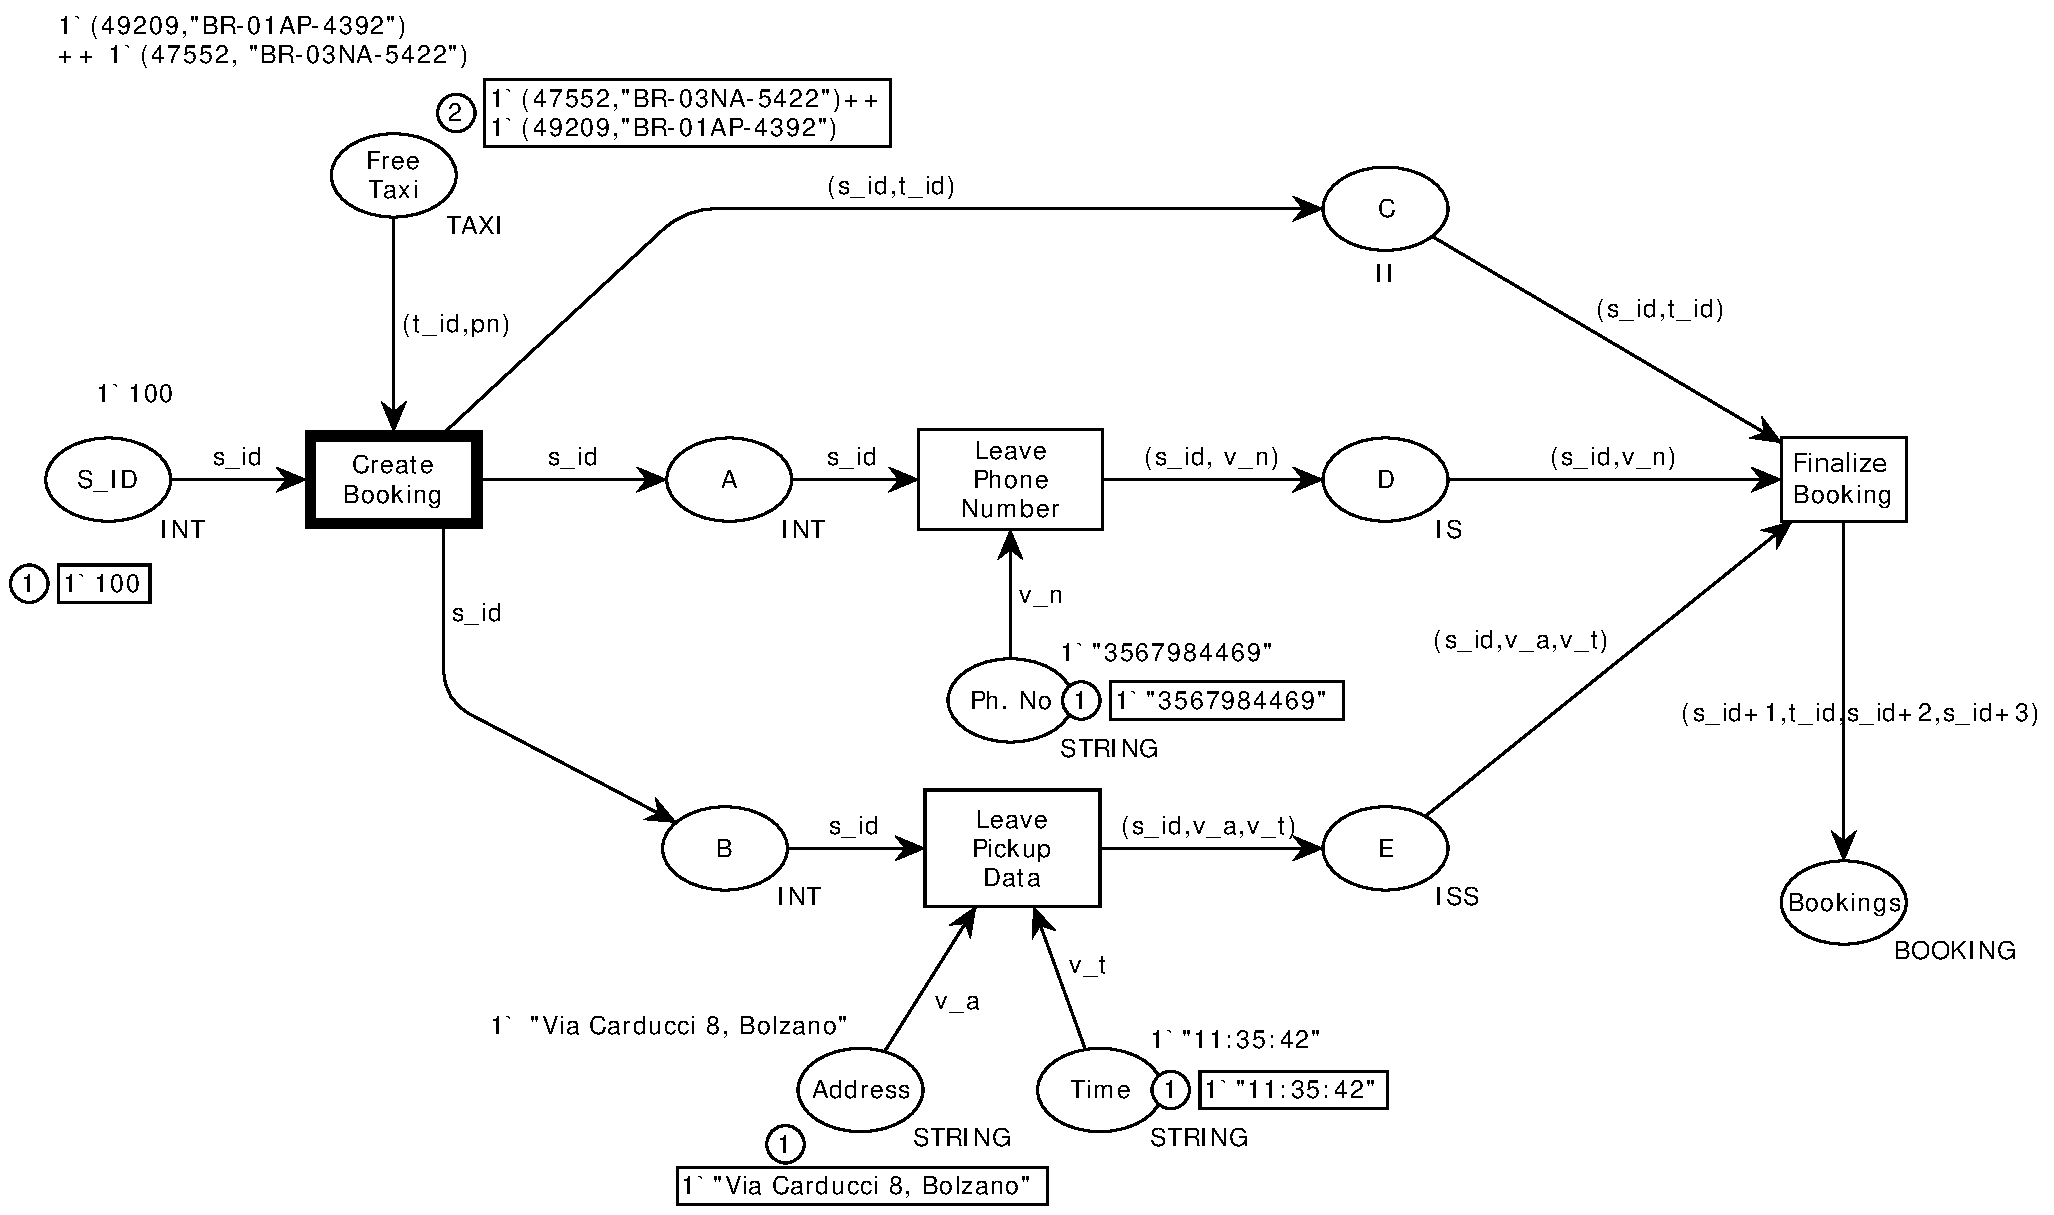
\includegraphics[scale = 0.4]{CPN_Taxi_Booking_simple.pdf}
	\caption{Revised CPN model showing a state for taxi booking example}
	\label{fig:CPN_Taxi_Booking_simple}
\end{figure}

\begin{figure}
	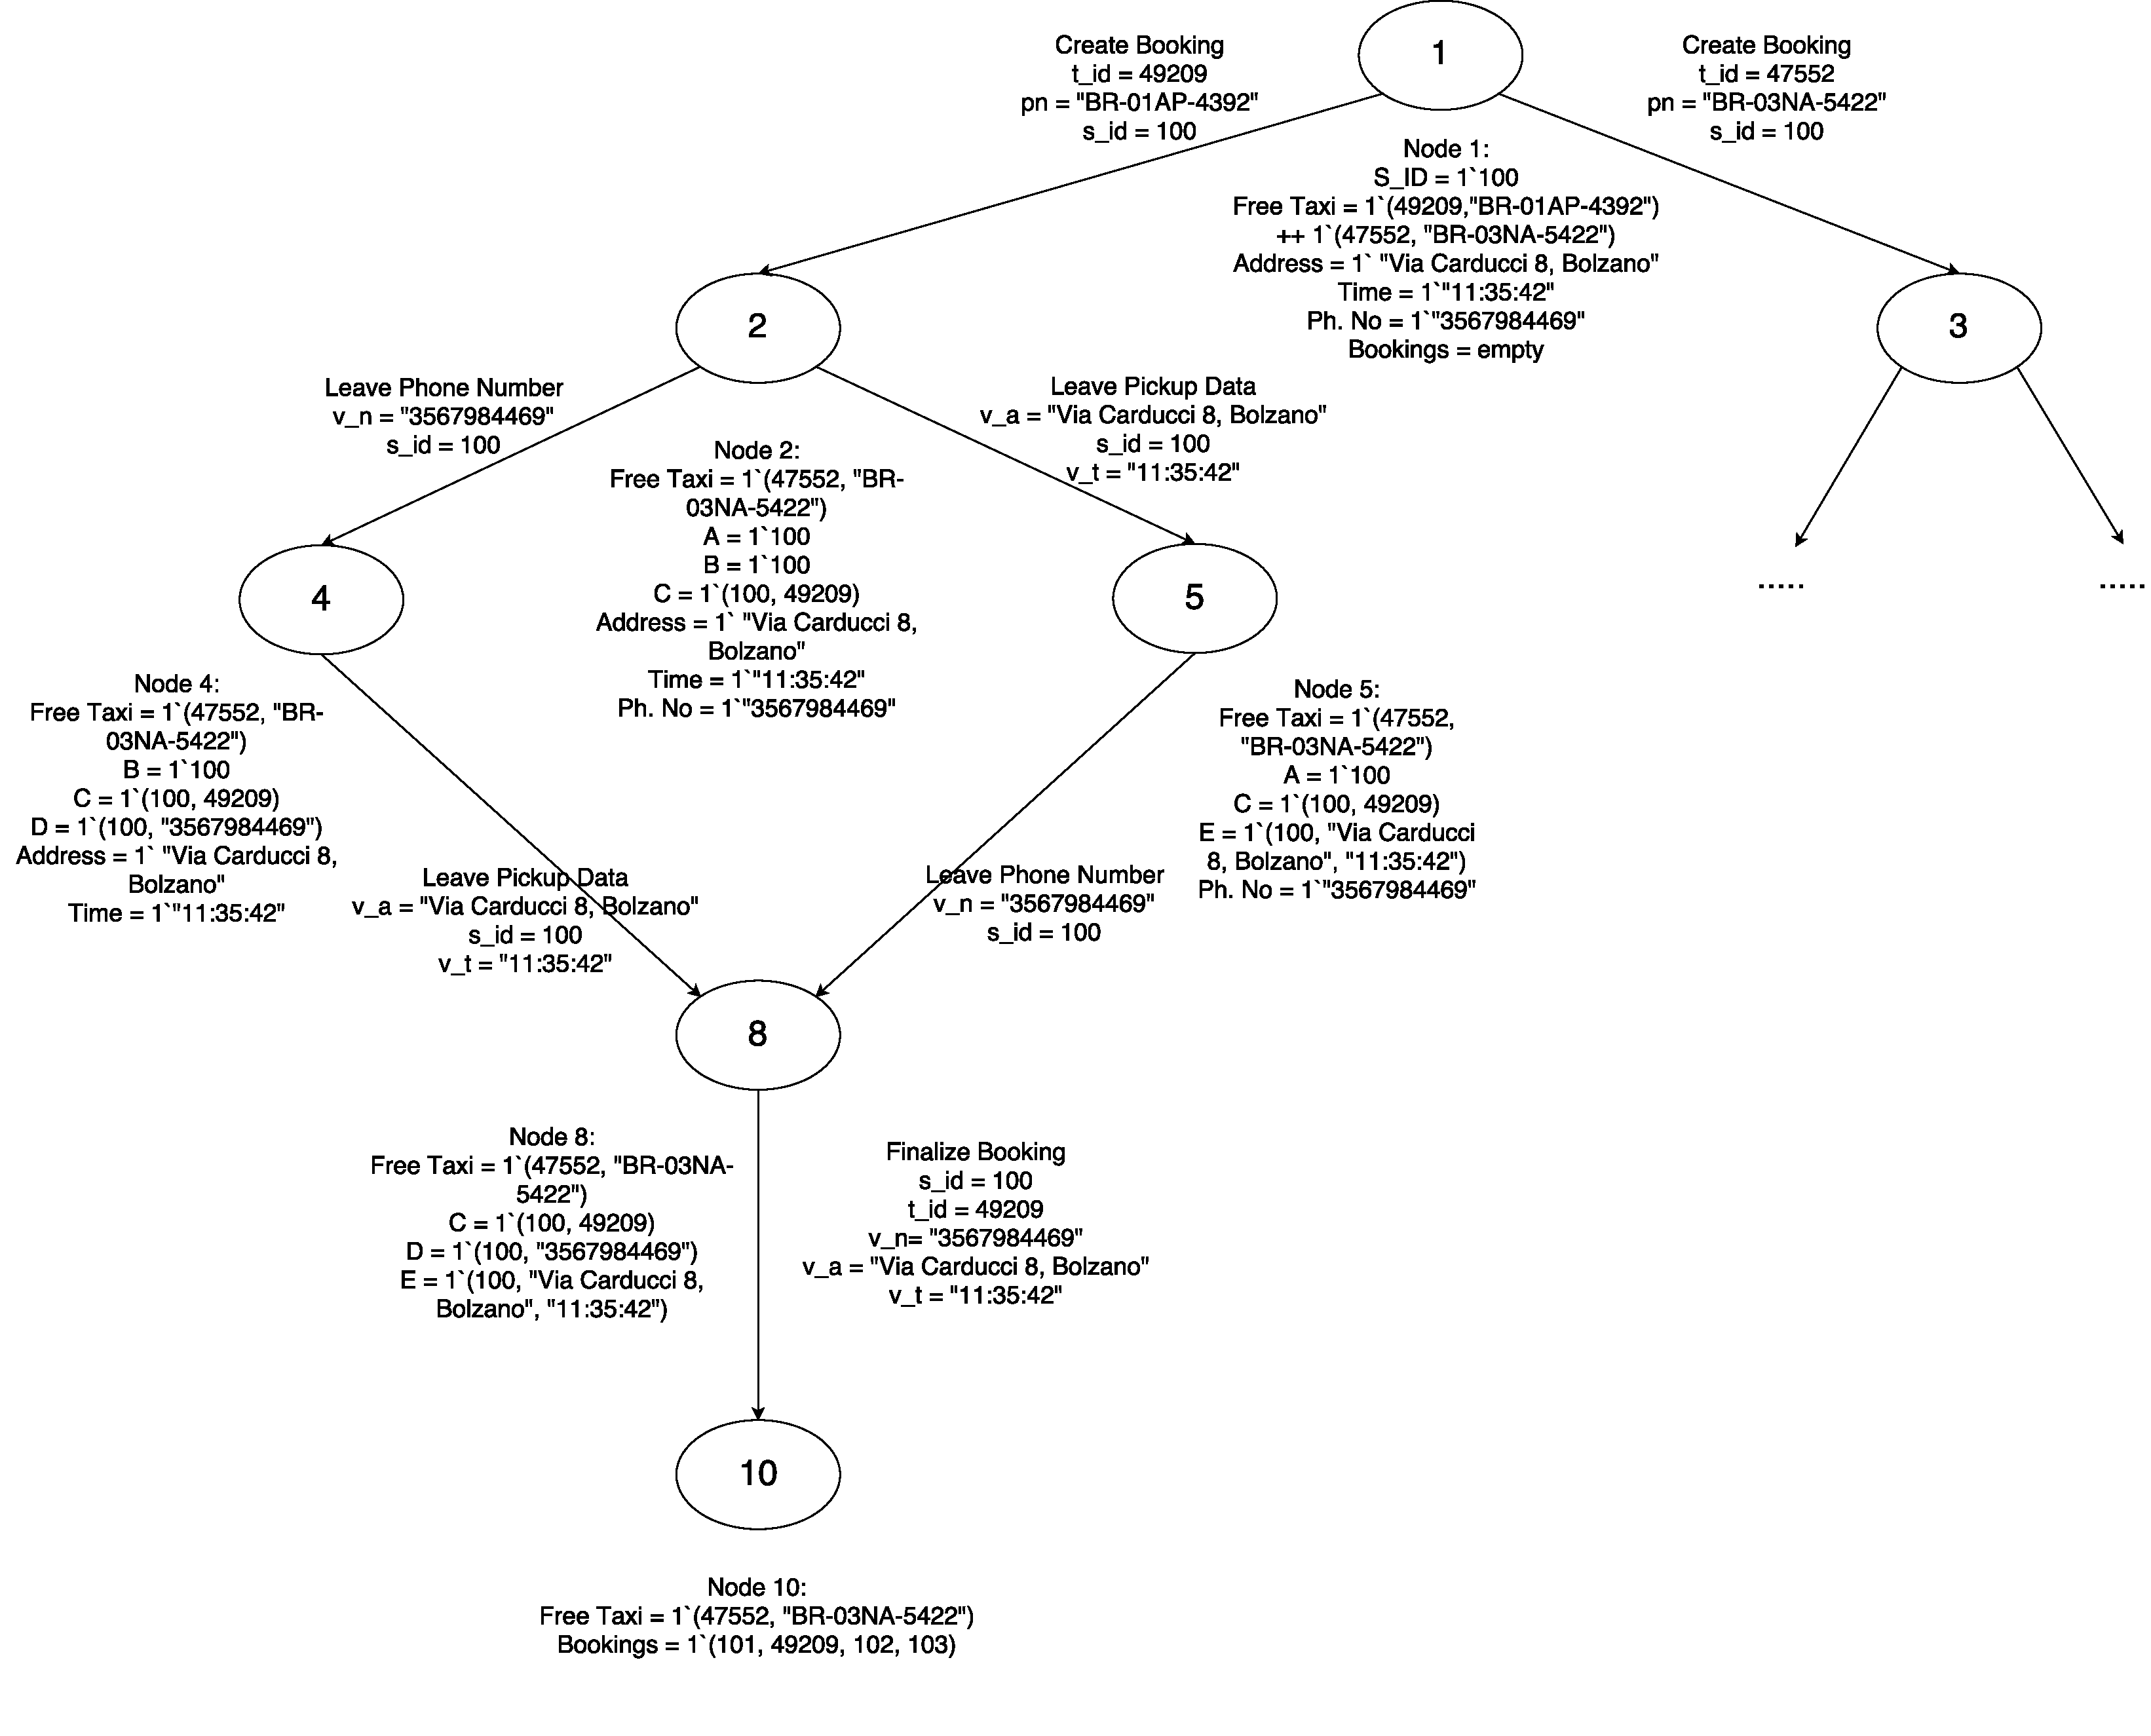
\includegraphics[scale = 0.21]{CPN_Taxi_Booking_State_Space.pdf}
	\caption{State Space for CPN model in Figure \ref{fig:CPN_Taxi_Booking_simple}}
	\label{fig:CPN_State_Space}
\end{figure}

\graphicspath{{./images/DBN/}}
\chapter{Extending CPN with Relational Data}
\label{ch:EXT_CPN_RDB}
\paragraph*{\textnormal{This chapter presents an extension of CPN with relational data. An attempt to integrate master data with processes, made by Montali and Rivkin in \cite{DBLP:journals/corr/DBNets}, is presented in this chapter. In this chapter, we will see how coloured petri nets can be extended in order to incorporate relational data. We first give an idea about different layers of DB-nets and how they are interconnected. Later, we will walk through the taxi booking example and modify it to adjust to a DB-net model. Finally, we model the developed DB-net model into CPN Tools. The example for the taxi booking model presented in this chapter is taken from \cite{DBLP:journals/corr/DBNets}.}}

\section{DB-Nets}
\paragraph*{\textnormal{In this section we will build up on the taxi booking example provided in the previous chapter. In this example, the process experts\footnote{process experts are people who are experts on modelling processes.} focus on how the process of booking a taxi is carried out. They may use the petri net model (informally presented in Figure \ref{fig:DBN_PN_Informal}) in order to represent the business process and its requirements, whereas on the other hand the master data experts would take care of requirements about the relevant data of the domain. Then, one can structure the data into classes, provide relationship, constraint etc in order to draft a database schema (informally represented in Figure \ref{fig:DBN_DataModel_Informal}).}}
\begin{figure}[!htbp]
	\centering
	\begin{subfigure}{0.5\textwidth}
		\centering
		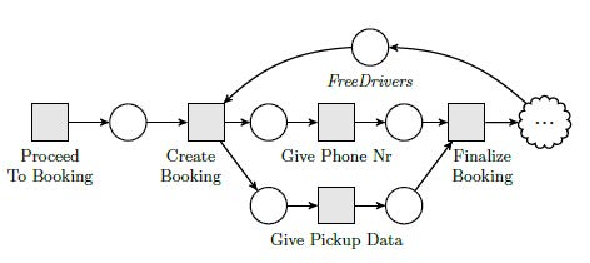
\includegraphics[width=1.0\linewidth]{DBN_PN_Informal.pdf}
		\caption{Process Model}
		\label{fig:DBN_PN_Informal}
	\end{subfigure}%
	\begin{subfigure}{0.5\textwidth}
		\centering
		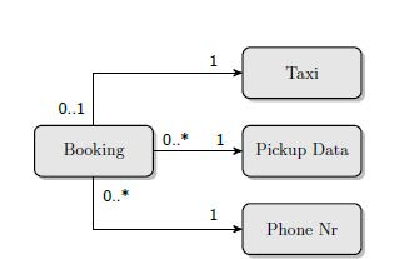
\includegraphics[width=0.7\linewidth]{DBN_DataModel_Informal.pdf}
		\caption{Data Model}
		\label{fig:DBN_DataModel_Informal}
	\end{subfigure}
	\caption{Figure \ref{fig:DBN_PN_Informal} captures the process part informally whereas figure \ref{fig:DBN_DataModel_Informal} captures the data model informally for the taxi booking example.}
	\label{fig:DBN_informal_model}
\end{figure}

\subparagraph*{\textnormal{The problem of integration lies in the example, that in the process flow, while encountering the \textit{Create Booking} transition the process expert would think to create a booking (i.e. instantiate the booking class), whereas from the schema, a booking can only exist in the database only if the corresponding taxi, phone number and the pickup address is provided. With this prospect, during execution one could keep track of free taxi, pickup data and phone number using local variables, and when \textit{Finalize Booking} is called, the corresponding booking entry is created. In this regard, we introduce DB-Nets. In Figure \ref{fig:DBN_Framework}, the framework of the db-nets is presented.}}

\begin{figure}[!htbp]
	\centering
	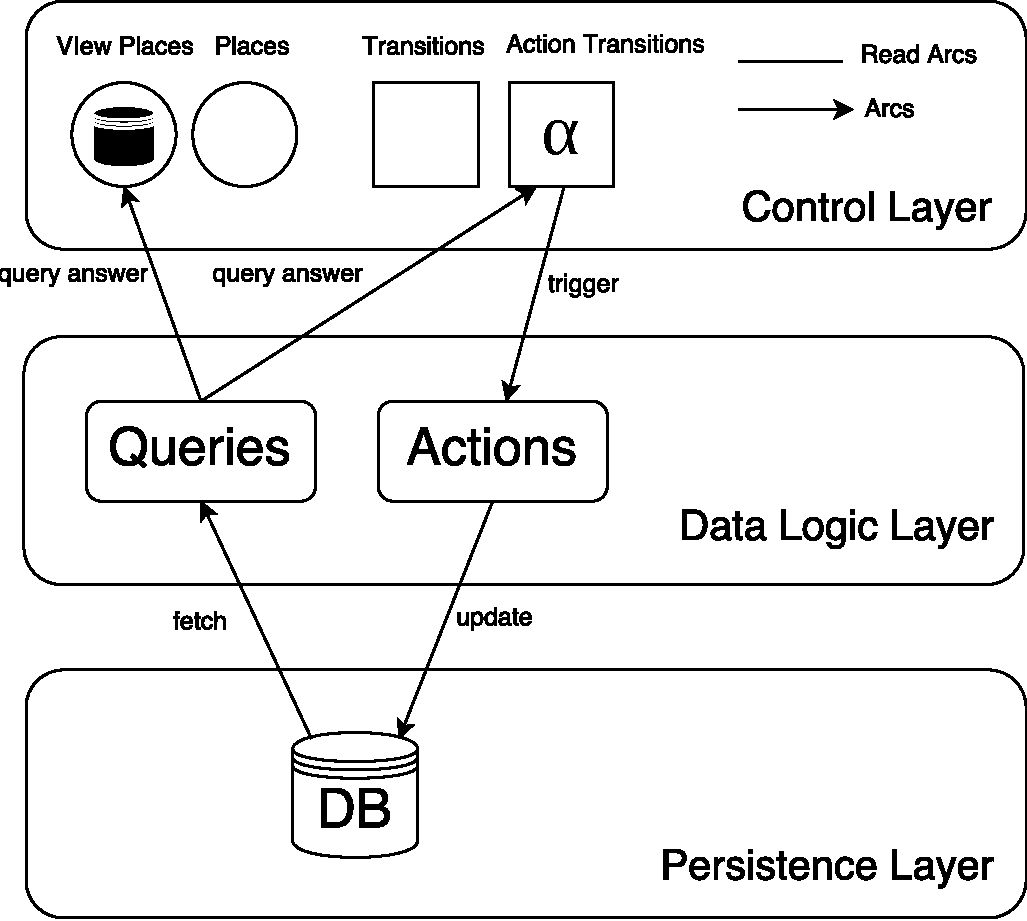
\includegraphics[scale = 0.35]{DBN_Framework.pdf}
	\caption{Framework of the DB-Net model}
	\label{fig:DBN_Framework}
\end{figure}

\subparagraph*{\textnormal{As per \cite{DBLP:journals/corr/DBNets}, the framework comprises of the three layers which are as follows:
		\begin{itemize}
			\item Persistence Layer - contains the full-fledged relational database with constraints. 
			\item Control Layer - process logic is represented with the help of a variant of CPN which supports:
			\begin{enumerate}
				\item typing of tokens, so
				as to account for local variables attached to execution threads.
				\item injection of possibly fresh data values via special so-called $\mathit{\nu}$-variables (leveraging the $\mathit{\nu}$-PN
				model \cite{DBLP:journals/tcs/Rosa-VelardoF11}).
				\item accessing the content of the underlying data layer via special	\textbf{\textit{view-places}}.
				\item updating the underlying data layer by attaching a database update logic to its transitions.
			\end{enumerate} 
			\item Data Logic Layer - used to connect the persistence and the control layer.
		\end{itemize}
}}
\subparagraph*{\textnormal{In figure \ref{fig:DBN_Framework}, the control layer contains a special place called view place, special transitions called action transitions and special arcs called read arcs. The control layer makes use of these special elements to interact with data logic layer in a bidirectional way.}}

\begin{comment}
If we don't intend to consume tokens from a place, then we connect the place with the read arc. The read arc just reads the token value and doesn't remove token from the connected place. The role of rollback arc is to undo the effect of a transition. We would discuss more about this later in the chapter.
\end{comment}

\subparagraph*{\textnormal{The db-net model of the taxi booking example is shown in Figure \ref{fig:DBN_Taxi_Example}. In this example, we assume that from some workflow  \textit{Proceed To Booking} transition is called. Similarly, after the booking is added there may be another workflow. In this example, we are only concerned about the workflow of booking a taxi. Let us see how the three layers (mentioned in the in figure \ref{fig:DBN_Framework}) can be interpreted in the given example (figure \ref{fig:DBN_Taxi_Example}).}}

\begin{figure}[!htbp]
	\centering
	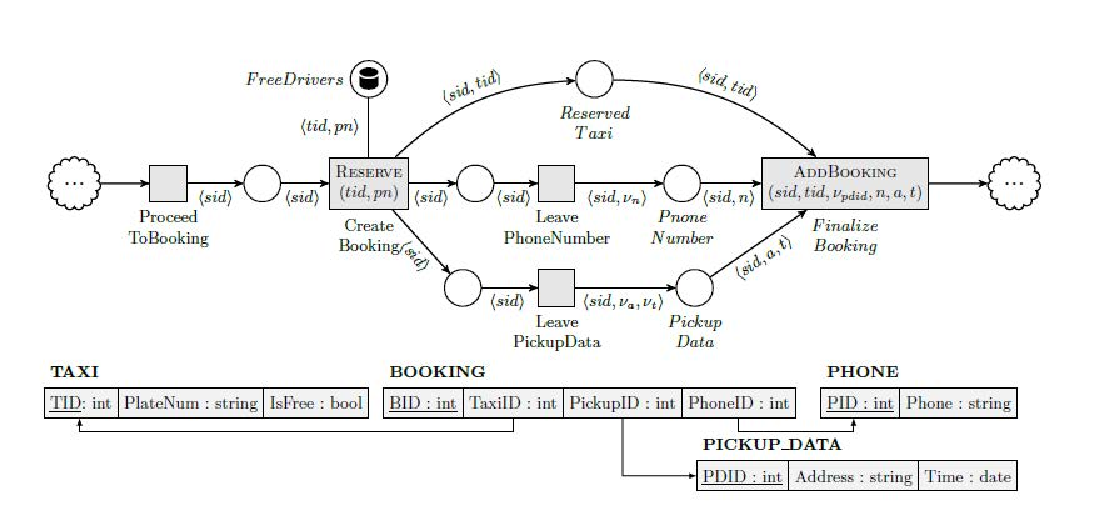
\includegraphics[scale = 0.8]{DBN_Taxi_Example.pdf}
	\caption{A db-net representing the taxi booking process}
	\label{fig:DBN_Taxi_Example}
\end{figure}

\subsubsection{Persistence Layer}
\begin{comment}
\paragraph*{\textnormal{Persistence layer consists of a full-fledged relational databases including constraints. For example, in figure \ref{fig:DBN_Taxi_Example}, the persistence layer consists of the database which contains table \bsq{\textbf{TAXI}}, \bsq{\textbf{BOOKING}}, \bsq{\textbf{PHONE}} and \bsq{\textbf{PICKUP\_DATA}}. The \bsq{TAXI} table consists of 3 columns \bsq{TID} containing integers, \bsq{PlateNum} containing strings and \bsq{IsFree} which contains the boolean value. If a taxi is available then its corresponding record in the \bsq{TAXI} table will have the column $IsFree = \textit{True}$. \bsq{PHONE} table consists of columns \bsq{PID} containing integers and \bsq{Phone} containing the phone numbers as strings. \bsq{PID} is the phone id for a particular phone number. \bsq{PICKUP\_DATA} table contains the pickup data for the customer. The columns in this table are \bsq{PDID} which contains integer, \bsq{Address} containing pickup address as string and \bsq{Time} of type date. \bsq{PDID} is the pickup id for a particular customer's pickup details (address and time). The table \bsq{BOOKING} contains the column \bsq{BID} as integer, \bsq{TaxiID} as integer, \bsq{PickupID} as integer and \bsq{PhoneID} as integer. For a particular record in the \bsq{BOOKING} table, \bsq{BID} denotes the corresponding booking id.}}

\subparagraph*{\textnormal{Along with the table structure, we have also introduced the constraints over it. For example, in the taxi table, a particular \bsq{TAXI} can be uniquely determined from \bsq{TID}. Hence, \bsq{TID} is the primary key (underlined in the figure \ref{fig:DBN_Taxi_Example}). Similarly, each phone number in the \bsq{PHONE} table can be determined by \bsq{PID} and in the table \bsq{PICKUP\_DATA} the pickup details can be determined by \bsq{PDID}. So, these two columns are marked as primary keys. In the \bsq{BOOKING} table, each booking can be determined by \bsq{BID}. \bsq{TaxiID}, \bsq{PickupID} and \bsq{PhoneID} are the foreign keys to the columns \bsq{TID}(in the \bsq{TAXI} table), \bsq{PDID}(in the \bsq{PICKUP\_DATA} table) and \bsq{PID}(in the \bsq{PHONE} table) respectively. This constraints will allow a booking to be added only if it has its corresponding \bsq{TaxiID}, \bsq{PickupID} and \bsq{PhoneID} in the \bsq{TAXI}, \bsq{PICKUP\_DATA} and \bsq{PHONE} table respectively.}}
\end{comment}

\subparagraph*{\textnormal{The persistence layer stores the relevant data for the domain of interest. We consider the relational databases along with its constraints. Using FOL we can express keys, functional dependencies and constraints over the database \cite{BagheriHariri}. For example, in Figure \ref{fig:DBN_Taxi_Example}, different tables are shown along with their functional dependencies and keys. A slight modification in persistence layer is presented in \cite{DBLP:journals/corr/DBNets}.}}

\subparagraph*{\textnormal{As mentioned in the preliminaries (section \ref{sec:preliminaries_relational_db_schema}), we consider the notion of relational schema, sort function and database schema for our need. }}

\begin{comment}
\subparagraph*{\textnormal{We will start with the definition of data type and adopt database schema and relational schema accordingly.}}
\subparagraph*{\textnormal{\todo{here these notions come out of the blue}Inspired from \cite{DBLP:books/aw/found_DB}, we assume \textit{domain} as a countably infinite set $\mathit{\Delta}$, \textit{attributes} as a finite set \textit{\mathit{U}}, and a mapping function $\mathit{dom:U\rightarrow\Delta$ and $dom(A)}$ is called domain of $\mathit{A}$, where $\mathit{A \in U}$.}}

\begin{defs}
\label{defs:dbn_sort_function}
\todo{for all the definitions, please, read carefully page 31 of the cited book. also, try to add more details to your definitions. for example, what does a finitary powerset mean?}
A function \textit{sort} is defined as $sort:R^{n}\rightarrow{\mathcal{P}^{fin}}(U)$, where ${\mathcal{P}^{fin}}$ is the finitary powerset\footnote{the set of finite subsets} of attributes, $R^{n}$ is the set of relation schema and $U$ is the finite set of attributes.
\end{defs}

\subparagraph*{\textnormal{The sort of a relation schema \textit{\mathit{R}} is simply written as $\mathit{sort(R)}$ and the arity is written as $\mathit{arity(R) = |sort(R)|}$. A relational schema ($\mathit{R}$) and set of attributes($\mathit{U}$) together make up the structure of the table. $\mathit{R[U]}$ is used to represent $\mathit{sort(R) = U}$, and $\mathit{R[n]}$ to represent $\mathit{arity(R) = n}$.}}

\begin{defs}
\label{defs:dbn_database_schema}
For a given domain $\Delta$, a \textbf{database schema}\todo{you haven't defined a type function for the database schema} is a non empty finite set $\mathcal{R}$ of relational schemas, written as:
\begin{equation*}
\mathcal{R} = \{R_{1}[U_{1}],\ldots,R_{n}[U_{n}]\}
\end{equation*}
where $R_{1},\ldots,R_{n}$ are relational schemas and $U_{1},\ldots,U_{n}$ are attributes
\end{defs}

\subparagraph*{\textnormal{For example, let \textbf{\textit{taxi\_booking}} be our database schema, shown in Figure \ref{fig:DBN_CPNTools_Taxi_Example}, which is defined by:
\begin{equation*}
\begin{aligned}
\textbf{\textit{taxi\_booking}} =& \{TAXI,\ BOOKING,\ PHONE,\ PICKUP\_DATA\}
\end{aligned}
\end{equation*}
where relational schemas TAXI and PHONE\footnote{One could also write sorts for other relation schemas in the $\textbf{taxi\_booking}$ schema} have the following sorts:
\begin{equation*}
\begin{aligned}
sort(TAXI) = & \{TID,\ PlateNum,\ IsFree\}\\
sort(PHONE)= & \{PID,\ Phone\}
\end{aligned}
\end{equation*}
}}

\subparagraph*{\textnormal{We assume that a \textit{data type} is an infinite set and is defined in a set theoretic manner. For example, \textit{int}, \textit{strings} etc. are \textit{data types}. We define a finite set $\mathit{\Gamma}$ as the set of all data types.}}

\begin{defs}
	\label{defs:dbn_type_function_database}
	A function $\mathit{type_{d}:U \rightarrow \Gamma}$, where $\mathit{U}$ is the set of attributes and $\mathit{\Gamma}$ is the set of data types.
\end{defs}

\subparagraph*{\textnormal{Now we define a typed relational schema as:}}

\begin{defs}
	\label{defs:dbn_typed_relational_schema}
	Given a relation schema $\mathit{R}$ and $\mathit{type_{d}}$ function, a typed relation schema $\mathit{R_{\Delta}}$ is a pair $\mathit{\langle R, type_{d}\rangle}$. 
\end{defs}

\subparagraph*{\textnormal{We extend the notion of the function $\mathit{sort}$, and we define a function $\mathit{sort_{d}}$, such as: }}

\begin{defs}
	\label{defs:dbn_typed_sort_function}
	A function $\mathit{sort_{d}}$ is defined as $\mathit{sort_{d}:R_{\Delta}^{n}\rightarrow{\mathcal{P}^{fin}}(U)}$, where $\mathit{{\mathcal{P}^{fin}}}$ is the finitary powerset\footnote{the set of finite subsets} of attributes, $\mathit{R_{\Delta}^{n}}$ is the set of typed relation schema and $\mathit{U}$ is the finite set of attributes.
\end{defs}

\subparagraph*{\textnormal{The typed sort of a relation schema $\mathit{R_{\Delta}}$ is simply written as $\mathit{sort(R_{\Delta})}$ and the arity is written as $\mathit{arity(R_{\Delta}) = |sort(R_{\Delta})|}$. A typed relational schema ($\mathit{R_{\Delta}}$) and set of attributes($\mathit{U}$) together make up the structure of the table. $\mathit{R_{\Delta}[U]}$ is used to represent $\mathit{sort(R_{\Delta}) = U}$.}}

\begin{defs}
	\label{defs:dbn_typed_database_schema}
	For a given domain $\mathit{\Delta}$, the set of data types $\mathit{\Gamma}$, a \textbf{typed database schema} is a non empty finite set $\mathit{\mathcal{R}_{\Delta}}$ of relational schemas, written as:
	\begin{equation*}
	\mathcal{R}_{\Delta} = \{R_{\Delta_{1}}[U_{1}],\ldots,R_{\Delta_{n}}[U_{n}]\}
	\end{equation*}
	where $\mathit{R_{\Delta_{1}},\ldots,R_{\Delta_{n}}}$ are typed relational schemas and $\mathit{U_{1},\ldots,U_{n}}$ are attributes.
\end{defs}
\end{comment}

\subparagraph*{\textnormal{For example, let \textbf{\textit{taxi\_booking}} be our database schema($\mathcal{R}$), shown in Figure \ref{fig:DBN_Taxi_Example}, which is defined as:
		\begin{equation*}
		\begin{aligned}
		\textbf{\textit{taxi\_booking}} =& \{TAXI,\ BOOKING,\ PHONE,\ PICKUP\_DATA\}
		\end{aligned}
		\end{equation*}
		where relational schemas TAXI and PHONE\footnote{One could also write sorts for other relation schemas in the $\textbf{taxi\_booking}$ schema} have the following sorts and data types:
		\begin{equation*}
		\begin{aligned}
		sort(TAXI) = & \{TID,\ PlateNum,\ IsFree\}\\
		sort(PHONE)= & \{PID,\ Phone\}\\\\
		dom(TID) =\ & int\\
		dom(PlateNum)=\ & string
		\end{aligned}
		\end{equation*}
}}

\begin{defs}
	\label{defs:dbn_rfacts}
	Given a database schema $\mathit{\mathcal{R}}$, a typed relation schema $\mathit{R}$, \textbf{an $\mathit{\mathcal{R}}$ fact} is of the form $\mathit{R(o_{1},\ldots,o_{n})}$ such that $\mathit{o_{i}}$ is an element of a data type and $\mathit{arity(R) = n}$.
\end{defs}

\subparagraph*{\textnormal{Here we will consider a full-fledged typed database schema as our persistence layer.}}
\subsubsection{Data Logic Layer}
\paragraph*{\textnormal{Data Logic Layer is the bidirectional interface between the control layer and the persistence layer. With bidirectional interface, we mean that on one hand we could extract data from an instance of the typed database schema which can be used in the persistence layer where as on the other hand, we could update the instance of the typed database schema by adding and deleting multiple facts at once. If the new database instance obtained after the update is compliant with the persistence layer, the update is committed, otherwise it is rolled back.}}

\subparagraph*{\textnormal{In order to query the database, we use first order logic queries, whereas to update the database instance, we follow the literature on data-centric processes \cite{DBLP:conf/icdt/Vianu09,DBLP:conf/pods/CalvaneseGM13}, where \textit{actions} are used to update database.}}

\begin{defs}
	An \textbf{action} over a persistence layer is a tuple $\mathit{\langle \textbf{n},\vec{p},F^{+},F^{-}\rangle}$, where $\mathit{\textbf{n}}$ is the action name, $\mathit{\vec{p}}$ is a tuple of pairwise distinct typed variables, denoting the \textit{action parameters}, $\mathit{F^{+}}$ and $\mathit{F^{-}}$ respectively represents a finite set of $\mathit{\mathcal{R}_{\Delta}}$-facts over $\mathit{\vec{p}}$, to be added or deleted from the current database instance.
\end{defs}

\subparagraph*{\textnormal{In order to access different components of the action $\mathit{\alpha = \langle \textbf{n},\vec{p},F^{+},F^{-}\rangle}$, we use the dot wise notation: $\mathit{\alpha\cdot}$name = \textbf{n}, $\mathit{\alpha\cdot}$params = $\mathit{\vec{p}}$, $\mathit{\alpha\cdot}$add = $\mathit{F^{+}}$, $\mathit{\alpha\cdot}$del = $\mathit{F^{-}}$. The data logic layer provides a set of actions with which one could update the database instance along with querying the database. For example, on firing the \textit{Create Booking} transition which contains the \textit{RESERVE} action, the database is updated such that the selected taxi is no longer available. The \textit{RESERVE} action has two input parameters, namely \textit{tid} and \textit{pn} denoting taxi id and the plate number respectively. This could be modelled as:
\begin{equation*}
\begin{aligned}
&RESERVE\cdot\textnormal{params} = \langle tid,pn \rangle \\
&RESERVE\cdot\textnormal{del} = \{Taxi(tid,pn,TRUE)\} \\
&RESERVE\cdot\textnormal{add} = \{Taxi(tid,pn,FALSE)\} \\
\end{aligned}
\end{equation*}
The set of FOL queries attached with the actions helps us querying the database and obtain the result. For example, the transition $\mathit{Finalize\ Booking}$, adds a booking to the table \textit{BOOKING} with a unique booking id, which is obtained as an answer to the attached query.}}

\subparagraph*{\textnormal{The data logic layer captures the flow of information from the control layer and performs actions on it. Similarly, this layer is also responsible for receiving the answer to the query from the persistence layer and passing on to the control layer.}}

\subparagraph*{\textnormal{Note that in control layer, we modify the definition of colour-sets ($\mathit{\Sigma}$) and say that colour-sets ($\mathit{\Sigma}$) is the finite set of possibly infinite colour-set. This is intentionally done to make the colour-sets compatible with answers of the queries.}}

\subsubsection{Control Layer}
\paragraph*{\textnormal{ In Figure \ref{fig:DBN_Framework}, the control layer has few additional components, namely, \textit{View places}, \textit{Action Transitions} and \textit{Read arcs}. These components are also incorporated in Figure \ref{fig:DBN_Taxi_Example}. The place $\mathit{Free\ Drivers}$ is a \textit{view place} which shows the currently available taxis. Since the records of the free taxi are stored in the database, they are fetched as an answer on querying the database. The set of view places is represented by $\mathit{P_{v}}$.}}

\begin{defs}
	\label{defs:dbn_query_function}
	A function $\mathit{query_{v}}$ is defined as $\mathit{query_{v} : P_{v} \rightarrow Q}$ where $\mathit{Q}$ is the set of first order logic queries.
\end{defs}

\begin{defs}
	\label{defs:dbn_formal_view_place}
	The set of \textbf{view places} ($\mathit{P_{v}}$) is a set such that:
	\begin{enumerate}
		\item $\mathit{P_{v} \subseteq P}$.
		\item for each $\mathit{p_{v} \in P_{v}}$, $\mathit{query_{v}(p_{v}) = q}$ where $\mathit{q \in Q}$.
		\item the answer $\mathit{(a_{1},\ldots,a_{k})}$ to the query $\mathit{q}$ having free variables $\mathit{(x_{1},\ldots,x_{k})}$, for all $\mathit{p_{v} \in P_{v}}$, $\mathit{(a_{1},\ldots,a_{k}) \in C(p_{v})}$.
		\item Let $\mathit{Ans = \{A_{1}, \ldots,A_{n}\}}$ be the set of answers returned for the query $\mathit{q}$ attached to the view place $\mathit{p_{v}}$, $\mathit{I(p_{v}) = {_{}^{++}\sum\limits_{A \in Ans}^{} {1}^{\backprime}A}}$.
	\end{enumerate}
\end{defs}

\subparagraph*{\textnormal{For example, $P_{v} = \{Free \ Drivers\}$ and for $p_{v} = Free \ Drivers$ we can attach a query to the view place as $query_{v} = Taxi(x,y,\textnormal{TRUE})$. Let us assume that there are two free taxis. The set of answers to the query \[Ans = \{(47552,\textnormal{\bdsq{BR-03NA-5422}}), (49209,\textnormal{\bdsq{BR-01AP-4392})}\}\]. The initialization function for the view place will be:
\begin{equation*}
\begin{aligned}
I(Free\ Drivers) =&\ 1^{\backprime} (47552,\textnormal{\bdsq{BR-03NA-5422}})\\
 &+\!\!+ 1^{\backprime} \textnormal{(49209,\bdsq{BR-01AP-4392}})
\end{aligned}
\end{equation*}
}}

\begin{comment}
\subparagraph*{\textnormal{For example, in order to show the available taxi one could show it by using the following query :}}

\begin{verbatim}
SELECT TID, PlateNum FROM TaxiBooking.TAXI WHERE IsFree = TRUE;
\end{verbatim}

\subparagraph*{\textnormal{In the SQL query above, TaxiBooking.TAXI represents the TAXI table of the schema TaxiBooking. So, it selects the taxi id(TID) and Plate Number(PlateNum), from the table TAXI which is the part of TaxiBooking schema, which is available ($\mathit{IsFree = True}$). Also, the query returns TID and PlateNum hence the colour-set of the view place should be compatible to the return type of the query. In this case the colour-set of the view place can be defined as:}}

\begin{verbatim}
COLSET TAXI = product INT * STRING;
\end{verbatim}

\begin{defs}
\label{defs:view_place}
A \textbf{view place} ($p_{v}$) extends the notion of a normal place in the CPN model. The extension is based on the following aspects:
\begin{enumerate}
\item A view place carry a database query with itself. The attached query should always be a SELECT clause.
\item The colour-set assigned to the view place should match with the data tuple resulted on answering the attached query.
\item View places are not immutable. It can change if the data in the data in the database changes.
\item View places should always be connected with read arcs.
\end{enumerate}
\end{defs}

\subparagraph*{\textnormal{We could formalize the notion of read arcs and view places.}}
\begin{defs}
\label{defs:read_arc}
A \textbf{read arc} extends the notion of a normal arc in the CPN model. The extension is based on the following aspects:
\begin{enumerate}
\item A read arc connects a transition and a view place.
\item In contrast to the normal arcs, the read arcs do not consume tokens from the view places. However, the free variables over the arcs are allowed to get assigned corresponding to an enabled binding if it exists.
\end{enumerate}
\end{defs}
\end{comment}

\subparagraph*{\textnormal{In Figure \ref{fig:DBN_Taxi_Example}, the view place is connected to the $\mathit{Create\ Booking}$ transition through a read arc. In contrast to a normal arc, instead of consuming tokens from the place, the read arc reads the token available at the view place. In the example, the inscription on read arc is $\mathit{\langle tid, pn \rangle}$. Similar to the normal arc, for an enabled binding element, the variables can take part in the assignment. The set of read arcs is represented by $\mathit{A_{r}}$.}}

\begin{defs}
	\label{defs:dbn_formal_read_arc}
	The set of \textbf{read arcs} $\mathit{A_{r}}$, where $\mathit{A_{r} \subseteq (P_{v} \times T) \cup (T \times P_{v})}$ such that:
	\begin{enumerate}
		\item $\mathit{A_{r} \subseteq A}$.
		\item $\mathit{A_{r}}$ is symmetric. i.e. $\mathit{(p_{v},t) \in A_{r}}$ iff $\mathit{(t,p_{v}) \in A_{r}}$ and $\mathit{E((p_{v},t)) = E((t,p_{v}))}$.
		\item For $\mathit{p_{v} \in P_{v}}$ and $\mathit{t \in T}$, $\mathit{(p_{v},t) \not\in (A\setminus A_r)}$ and $\mathit{(t,p_{v}) \not\in (A\setminus A_r)}$.
	\end{enumerate}
\end{defs}
\subparagraph*{\textnormal{The second condition in the Definition \ref{defs:dbn_formal_read_arc} states that, the read arcs cannot consume tokens whereas the third condition restricts \textit{view places} to connect with normal arcs. In the example (see Figure \ref{fig:DBN_Taxi_Example}), the set of read arcs is represented by :
		\begin{equation*}
		A_{r} = \{(Free \ Drivers, Create Booking),(Create Booking, Free \ Drivers) \}
		\end{equation*}}}

\subparagraph*{\textnormal{Along with carrying execution in CPN, the role of transitions in DB-nets are mainly:
		\begin{enumerate}
			\item acquire data from the environment using fresh variables.
			\item perform queries and updates on the persistence layer.
\end{enumerate}}}

\begin{defs}
	For a transition $\mathit{t \in T}$, the set of \textbf{output variables} $\mathit{Var_{out}[t]}$ is the set of variables such that for all pair $\mathit{(t,p) \in A}$, $\mathit{Var_{out}[t] = Var[E((t,p))]}$ where $\mathit{p \in P}$ and $\mathit{E}$ is the expression function.
\end{defs}

\begin{defs}
	For a transition $\mathit{t \in T}$, the set of \textbf{input variables} $\mathit{Var_{in}[t]}$ is the set of variables such that for all pair $\mathit{(p,t) \in A}$, $\mathit{Var_{in}[t] = Var[E((p,t)))]}$ where $\mathit{p \in P}$ and $\mathit{E}$ is the expression function.
\end{defs}

\begin{defs}
	For a transition $\mathit{t \in T}$, the set of \textbf{fresh variables} $\mathit{Var_{f}[t]}$ $\mathit{= Var_{out} \setminus Var_{in}}$.
\end{defs}

\subparagraph*{\textnormal{Note that the outgoing arc of \textit{LEAVE PHONE NUMBER} transition contains an additional variable $v_{n}$. The set of \textit{output variables}, \textit{input variables} and \textit{fresh variables} for \textit{LEAVE PHONE NUMBER} transition is:
\begin{equation*}
\begin{aligned}
&Var_{out}[t] = \{s\_id,v_{n} \} \\
&Var_{in}[t] = \{s\_id\} \\
&Var_{f}[t] = Var_{out}[t] \setminus Var_{in}[t] = \{v_{n}\}
\end{aligned}
\end{equation*}
%In order to avoid modelling complexities, we assume that the $\mathit{\mathcal{R}_\Delta}$ facts to be deleted in $\mathit{F^{-}}$ do not depend on fresh variables. 
Transitions are responsible for performing updates over the database. For example, the transition $\mathit{Create\ Booking}$ reserves the available taxi, and thus updates the database instance by making the selected taxi unavailable for further booking. We call these transitions as \textit{Action Transition}.}}

\begin{defs}
	\label{defs:DBN_transition_action_function}
	A function $\mathit{trans_{act}}$ is a function $\mathit{trans_{act} : T \rightarrow \Lambda}$ where $\mathit{T}$ is the set of transitions and $\mathit{\Lambda}$ is the set of actions.
\end{defs}
\begin{defs}
	\label{defs:dbn_formal_action_transition}
	The set of \textbf{action transitions} $\mathit{T_{a}}$ is a set such that:
	\begin{enumerate}
		\item $\mathit{T_{a} \subseteq T}$.
		\item for all $\mathit{t_{a} \in T_{a}}$, $\mathit{trans_{act}(t_{a})}$ is non-empty.
	\end{enumerate}
\end{defs}

\paragraph*{\textnormal{In the example shown, the set of \textit{action transitions} is given by:
\begin{equation*}
T_{a} = \{Proceed\ To\ Booking, Create\ Booking, Leave\ Phone\ Number, ...\}
\end{equation*}
The fresh variables are used for acquiring data from the external environment. Using all the definitions above we can now formalize the notion of a DB-Net(DBN).}}
\begin{defs}
	\label{defs:DBN_formal_definition_DBN}
	A non-hierarchical DBN is a fifteen-tuple\\{$\mathit{DBN = (P,P_{v},T,T_{a},A,A_{r},\Sigma,V,C,G,E,I,\mathcal{R}_{\Delta},query_{v},trans_{act})}$}, where:
	\begin{itemize}
		\item $\mathit{P,T,A,V,C,G,E,I}$ stands same as defined in CPN.
		\item $\mathit{\Sigma}$ is the finite set of possibly infinite colour-sets.
		\item $\mathit{P_{v}}$ is the set of view places such that $\mathit{P_{v} \subseteq P}$ and a first order logic query assigned to it.
		\item $\mathit{T_{a}}$ is the set of action transitions such that $\mathit{T_{a} \subseteq T}$, which contains actions required to query and update the database.
		\item $\mathit{A_{r}}$ is the set of read arcs such that $\mathit{A_{r} \subseteq A}$, which connects a view place to a transition.
		\item $\mathit{\mathcal{R}_{\Delta}}$ is the full fledged typed database schema.
		\item $\mathit{query_{v}}$, defined as $\mathit{query_{v} : P_{v} \rightarrow Q}$, where $\mathit{Q}$ is the set of FOL queries.
		\item $\mathit{trans_{act}}$, defined as $\mathit{trans_{act}: T \rightarrow \Lambda}$ is a function from the set of transitions to the set of actions.
	\end{itemize}
\end{defs}

\section{DB-Nets Modelling}
\paragraph*{\textnormal{In this section, we will see how to model a DB-Net using CPN Tools in an abstract manner. The DB-Net modelled in CPN Tools\footnote{To know how to use actions in transitions in CPN Tools \cite{CPN_Tools_CodeSegment}.} is shown in Figure \ref{fig:DBN_CPNTools_Taxi_Example}. In CPN Tools, read arcs are not provided. Therefore, instead of read arcs we use double headed arcs, which allow the consumption and regeneration of tokens at the place in a unit time. In this model the set of \textit{view places}, \textit{action transitions} and \textit{read arcs} is given by:
\begin{equation*}
	\begin{aligned}
		P_{v} =& \{Free \ Drivers\}\\
		T_{a} =& \{Create\ Booking, Leave\ Phone\ Number, Leave\ Pickup\ Data,\\
		& Finalize\ Booking\}\\
		A_{r} =& \{(Free \ Drivers, Create Booking),(Create Booking, Free \ Drivers) \}
	\end{aligned}
\end{equation*}
The query attached with the view place is given by:
\begin{equation*}
	query_{v}(Free\ Taxi) = Taxi(TID,PlateNum,TRUE)
\end{equation*}
where \textit{TID} and \textit{PlateNum} are the free variables in the query determining the corresponding taxi id and plate number of the available taxi. The variables of interest for the actions attached to the transitions are taken as parameter in the input clause. Fresh variables are specified in the output clause. For example, in the \textit{Finalize Booking} transition, the variables in the input clause are:
\begin{equation*}
	\{t\_id, v\_n, v\_a, v\_t\}
\end{equation*}
and the fresh variables (for booking id, pickup id and phone id) mentioned in the output clause are:
\begin{equation*}
	\{b\_id,pd\_id,ph\_id\}
\end{equation*}
In the action part, the fresh variables acquire their data from the external environment (e.g. getBookingID()). The \textit{INSERTPHONE} action adds a new entry in the table \textit{PHONE} with the corresponding phone number and the phone id. Note that, \textit{INSERTPHONE} action is followed by \textit{INSERTPICKUP} and \textit{INSERTBOOKING} action to obey the foreign key constraints. Similarly, in the \textit{Create Booking} transition, the \textit{RESERVE} action updates the database instance by making the selected taxi unavailable for further booking.}}

\begin{figure}[!htbp]
	\centering
	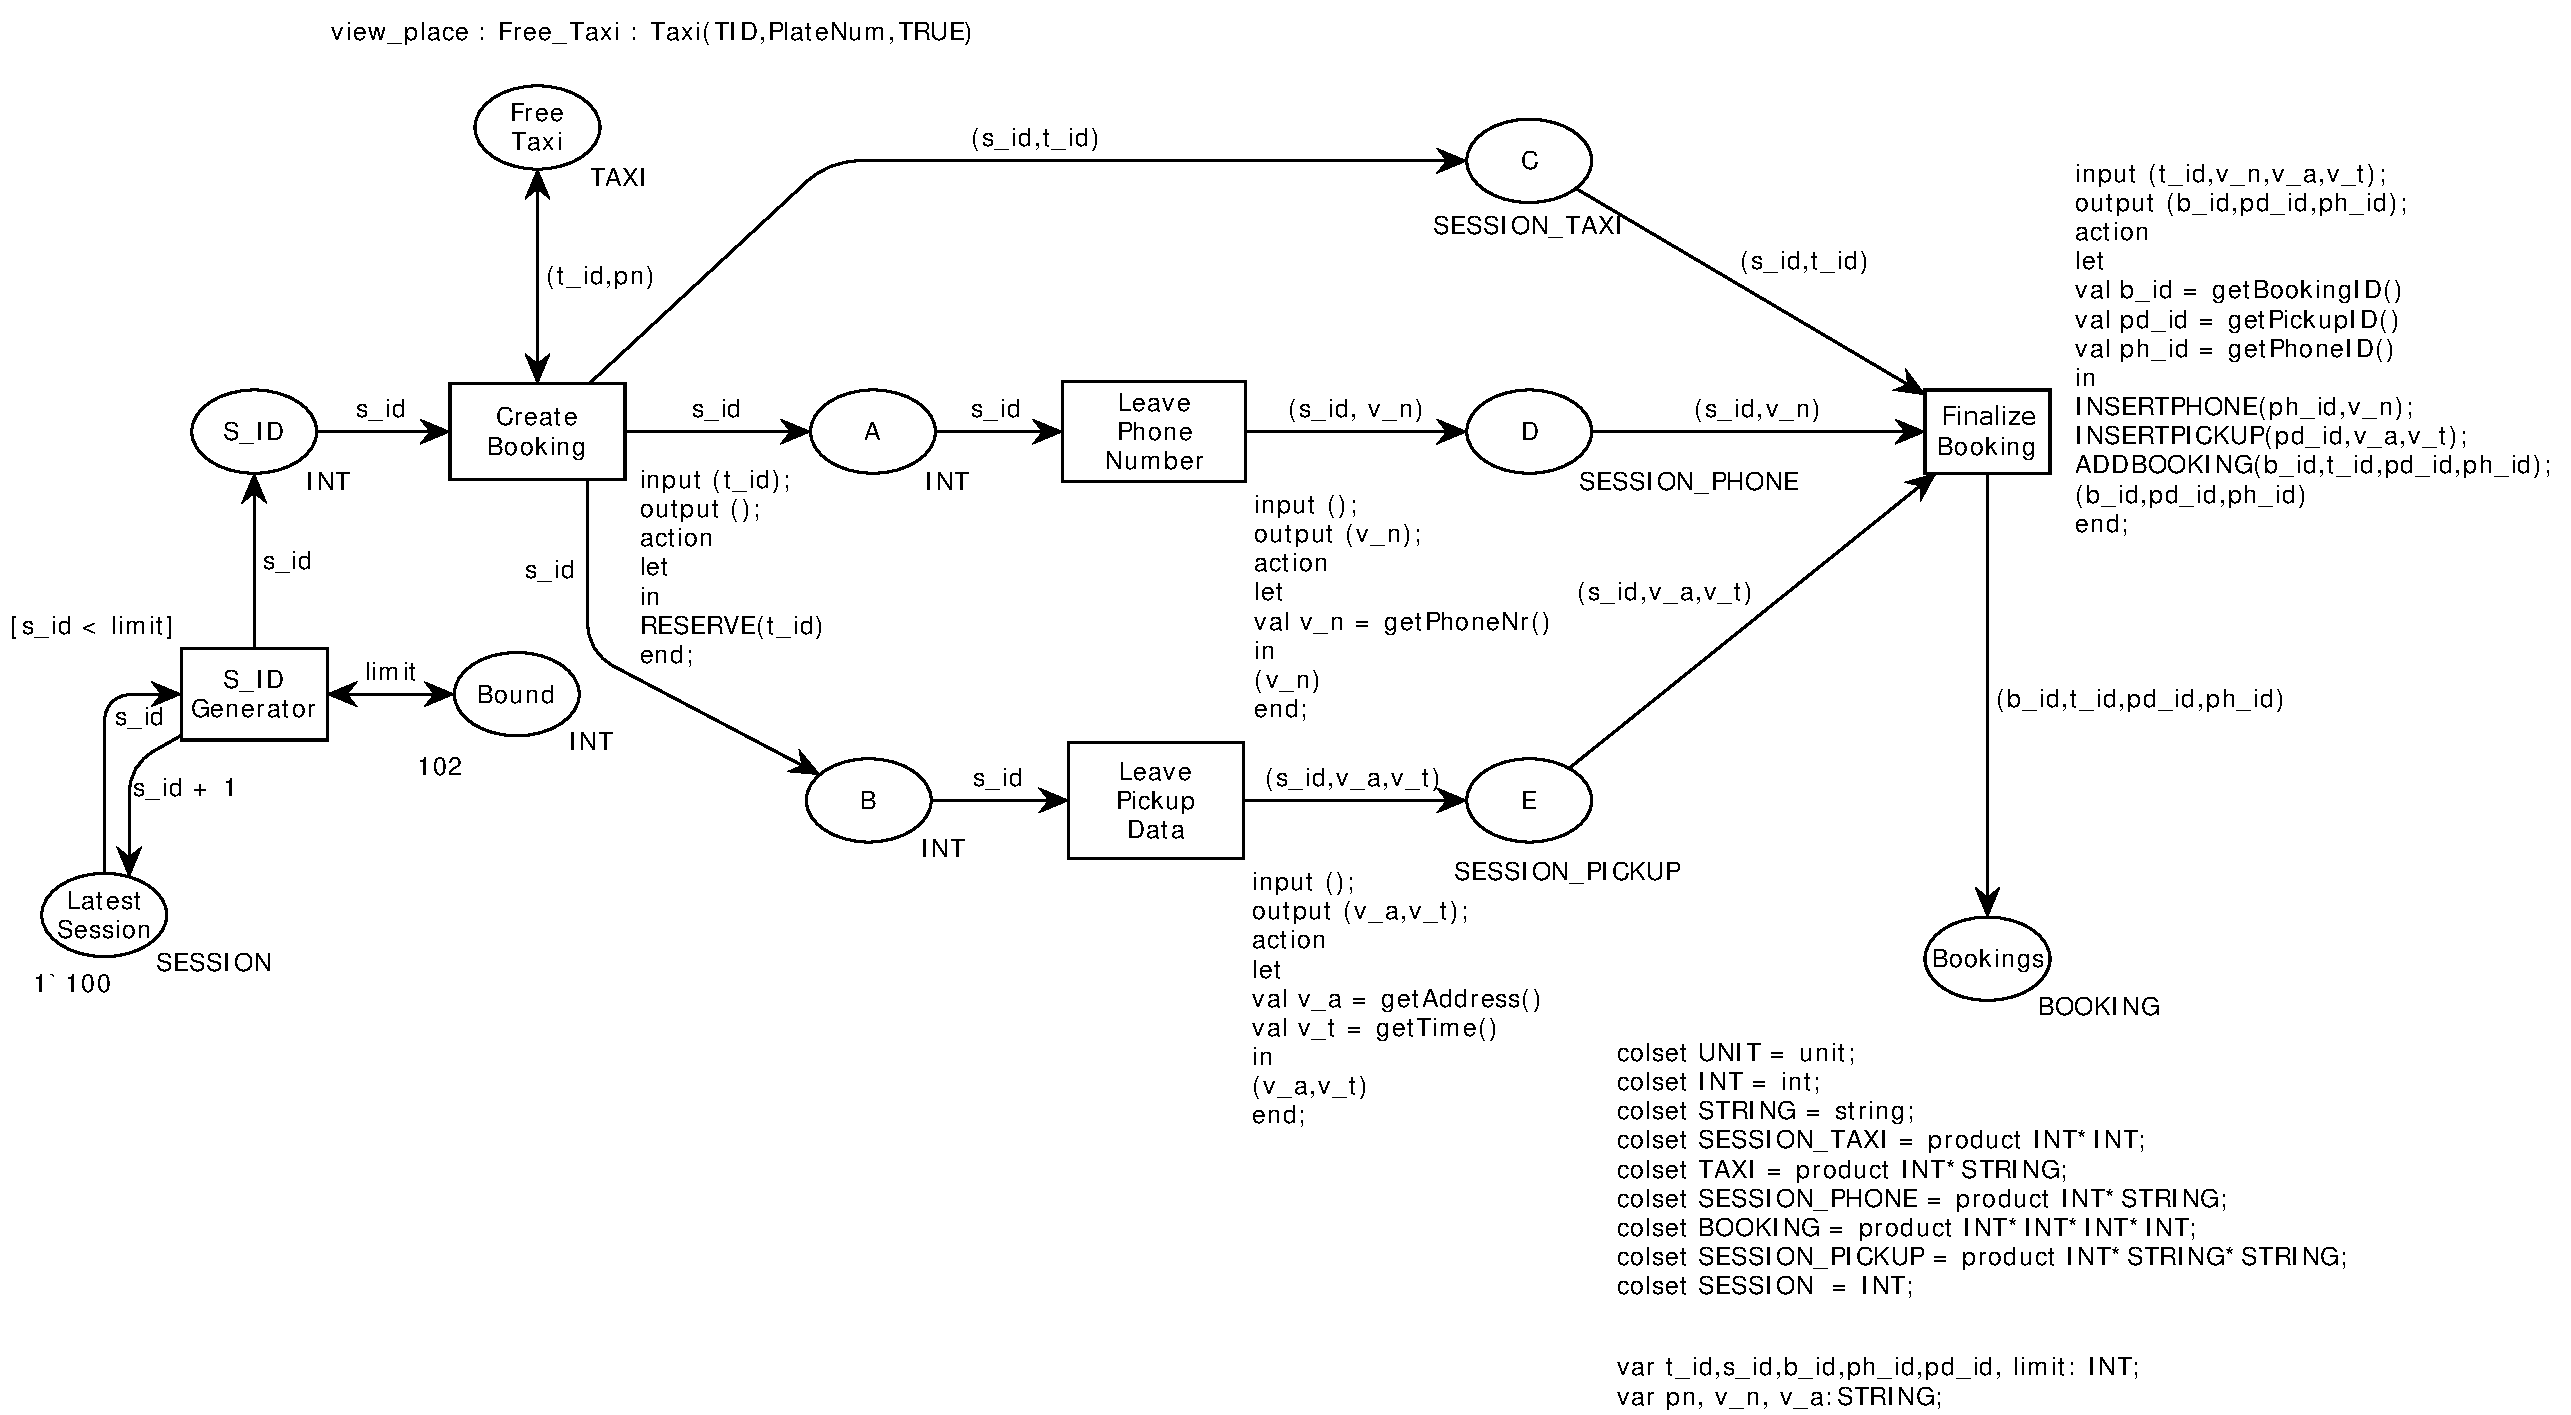
\includegraphics[scale = 0.33]{DBN_CPNTools_Taxi_Example.pdf}
	\caption{A db-net representing the taxi booking process modelled in CPN Tools}
	\label{fig:DBN_CPNTools_Taxi_Example}
\end{figure}

\subparagraph*{\textnormal{The major components in the DB-Nets are view places, read arcs, action transitions, the data logic layer and the data acquisition for fresh variables. Using these we could interact with the persistence layer. The execution semantics of CPNs can be applied over DBN. Additionally, after occurrence of every step, the view places need to be refreshed, e.g. the view place $\mathit{Free\ Taxi}$ needs to be updated when a step occurs in the net.}}

\subparagraph*{\textnormal{In the later chapters, we will see the development and working of the DB-Nets extension for CPN Tools.}}



\graphicspath{{./images/DBN_Impl/}}
\chapter{DB-nets Implementation: A CPN Tools Extension}
\label{ch:DBN_Impl}
\paragraph*{\textnormal{In this chapter, we discuss how DB-nets are modelled in CPN Tools and implemented using extension supported by CPN Tools. We develop an extension which implements the functionality of DB-nets in CPN Tools. First we provide a gentle introduction to CPN Tools extension and the framework that we adopt for implementing different aspects of DB-nets, e.g., action transitions, view places and data acquisition. Later, we present an architecture for the implementation of the different layers of DB-nets. We provide the communication pattern of our extension and briefly describe the program used for data acquisition and handling actions attached to transitions.}}
\subparagraph*{\textnormal{Considering the taxi booking example from the previous chapter, we gradually transform our CPN model to a DB-net model. We implement each of the layers independently and finally explain the connection between them. After transformation from the CPN model to the DB-net model, we can perform simulation over the transformed DB-net model.}}

\section{CPN Tools Extension}
\label{sec:DBN_Impl_CPN_Tools_Extension}
\paragraph*{\textnormal{As seen earlier, we use CPN Tools for modelling our CPN. CPN Tools has two major components:
\begin{itemize}
	\item GUI - the user interface, which provides us the functionality to model our CPNs.
	\item Simulator - which is responsible for simulation and analysis of CPNs.
\end{itemize}
The GUI of CPN Tools is written in BETA \cite{BETA} programming language and the simulator is written in SML \cite{milner1997definition}. The GUI of CPN Tools provides the functionality to draw net elements and the simulator keeps tracks of the declaration such as colour-sets and variables, ML functions, enablement and firing of transitions etc. CPN Tools (version 4) supports development of simulator extensions which help users to develop customized functionalities. Simulator extension \cite{CPN_Tools_Extension} has the possibility of adding functionalities using JAVA and also allows third parties to add functionalities without relying on BETA and SML programming languages. Simulator extensions, through JAVA programs provide control for numerous operations performed by the simulator.}}

\subsection*{Architecture}
%\label{subsec:DBN_Impl_CPN_Tools_Extension_Architecture}
\subparagraph*{\textnormal{In CPN Tools, modelling and execution of any CPN depends on the interaction between GUI and simulator (see Figure \ref{fig:DBN_Impl_CPN_Tools_Architecture}). Access/CPN \cite{AccessCPN} is a framework which facilitates the development of extensions in JAVA.
\begin{figure}[!htbp]
	\centering
	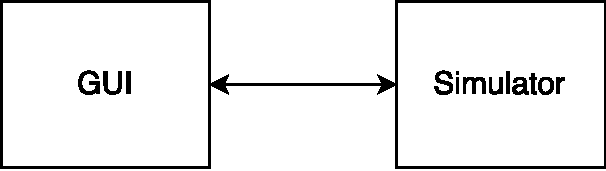
\includegraphics[scale = 0.35]{DBN_Impl_CPN_Tools_Architecture.pdf}
	\caption{Interconnectivity between CPN Tools GUI and Simulator}
	\label{fig:DBN_Impl_CPN_Tools_Architecture}
\end{figure}
Access/CPN consists of two interfaces, one is written in SML (which is close to the simulator) and the other in JAVA. The interface written in JAVA provides users with the possibility to access the simulator. Additionally the interface also provides an object oriented representation of the CPN models loaded in CPN Tools. With Access/CPN library \cite{AccessCPN_Library}, one could replace the GUI part with any component written in JAVA(see Figure \ref{fig:DBN_Impl_CPN_Tools_Architecture_Access_CPN}).
\begin{figure}[!htbp]
	\centering
	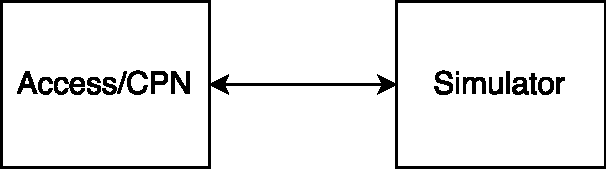
\includegraphics[scale = 0.35]{DBN_Impl_CPN_Tools_Architecture_Access_CPN.pdf}
	\caption{Interconnectivity between Access/CPN and Simulator}
	\label{fig:DBN_Impl_CPN_Tools_Architecture_Access_CPN}
\end{figure}
Using these libraries, one could develop simulator extensions in JAVA which are capable of communicating with CPN Tools Simulator and CPN Tools GUI (see Figure \ref{fig:DBN_Impl_CPN_Tools_Architecture_Extension}). The extension is directly connected with the simulator and any communication between extension and GUI takes place through the simulator. Thus, the simulator acts as a mediator between the GUI and extension.
\begin{figure}[!htbp]
	\centering
	
\includegraphics[scale = 0.35]{DBN_Impl_CPN_Tools_Architecture_Extension.pdf}
	\caption{Interconnectivity between GUI, Simulator and Extension}
	\label{fig:DBN_Impl_CPN_Tools_Architecture_Extension}
\end{figure}}}

\subparagraph*{\textnormal{Access/CPN provides a JAVA interface for an extension, which helps in accessing the \textit{channel} through which the communication takes place between the simulator and extension. The communication between components (GUI, simulator and extension) involves sending and receiving \textit{packets}\footnote{Packets generally contain messages in a specific format which are used to instruct the components to perform certain actions.} passing through the channel. This \textit{channel} is provided to the user in the \bsq{Extension} interface of Access/CPN. Access/CPN also provides subscription to specific events\footnote{A list of events which could be subscribed is provided in \cite{CPN_Tools_Message_Format}.} occurring in CPN Tools such as the firing of transitions, setting markings of places etc. One could listen to those events by subscribing through JAVA code (provided in the \bsq{Extension} interface of Access/CPN). Once the events are subscribed, one could \textit{handle} it (provided in the \bsq{Extension} interface of Access/CPN), and perform customised actions based on events. Various communication patterns which can be used are available in \cite{CPN_Tools_Extension}, however, for our extension, we adopt a customised communication pattern which is a mixture of patterns mentioned in \cite{CPN_Tools_Extension}.}}

\section{Comms/CPN}
\label{sec:DBN_Impl_Comms_CPN}
\paragraph*{\textnormal{Comms/CPN allows CPN Tools to communicate with external processes. Comms/CPN \cite{gallasch2001comms} is a Standard ML library that augments Design/CPN \cite{Design_CPN} with the necessary infrastructure to establish communication between CPN models and external processes. As described in \cite{Design_CPN}, Design/CPN is a tool package which supports modelling, simulation and verification by means of hierarchical CPNs. For modelling, simulation and verification purposes we already have CPN Tools and we connect it to external processes using Comms/CPN APIs. In our case, the external process is a JAVA application which is used to facilitate data acquisition and actions attached to transitions.}}

\begin{figure}[!htbp]
	\centering
	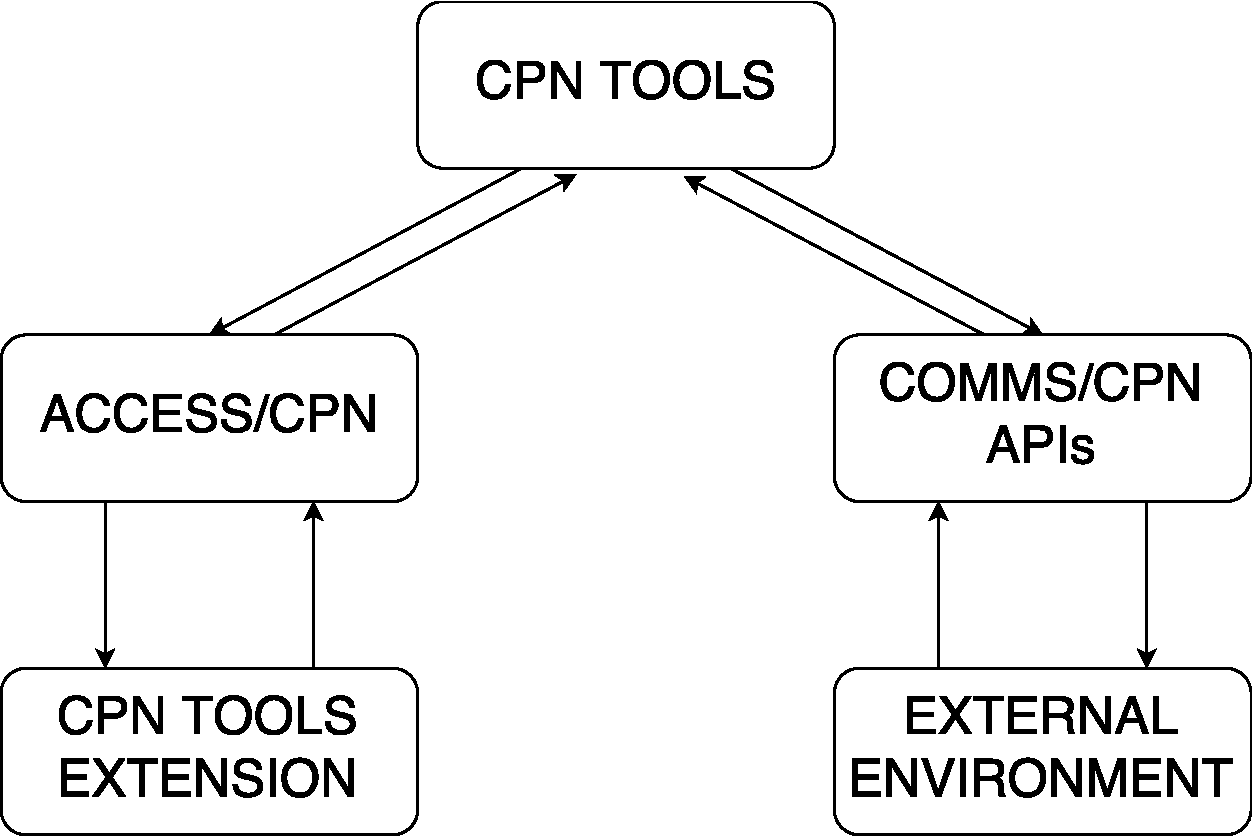
\includegraphics[scale = 0.35]{DBN_Impl_CPN_Tools_Extension_External_Environment.pdf}
	\caption{Connectivity between CPN Tools extension, external environment and CPN Tools}
	\label{fig:DBN_Impl_CPN_Tools_Extension_External_Environment}
\end{figure}

\subparagraph*{\textnormal{The Comms/CPN is implemented in a layered fashion as shown in Figure \ref{fig:DBN_Impl_COMMS_CPN_Layer} (taken from \cite{gallasch2001comms}). The topmost layer is the Connection Management Layer followed by Messaging Layer and the Communication Layer. The Comms/CPN uses TCP/IP protocol to send/receive messages in the form of stream of bytes over a specified port. Similarly, the external application connected to the specified port should also be able to send/receive messages using TCP/IP protocol. Using this architecture, Comms/CPN is able to establish communication between the CPN model and the external application.}}

\begin{figure}[!htbp]
	\centering
	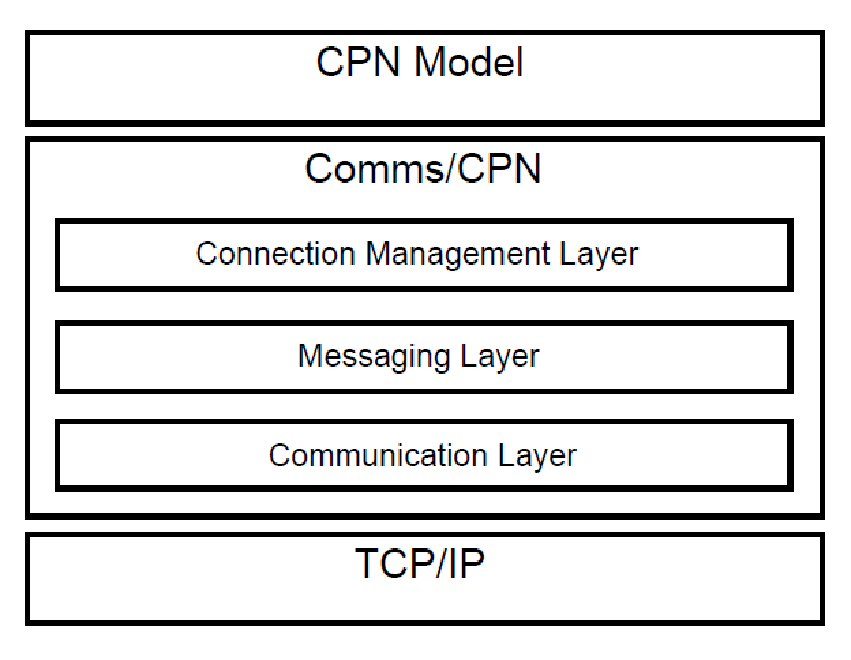
\includegraphics[scale = 0.35]{DBN_Impl_COMMS_CPN_Layer.pdf}
	\caption{Overall architecture of Comms/CPN}
	\label{fig:DBN_Impl_COMMS_CPN_Layer}
\end{figure}

\subparagraph*{\textnormal{JAVA/CPN\footnote{The source code of JAVA/CPN is provided in \cite{CPN_Tools_Comms/CPN}.}, a library written in JAVA, allows a JAVA process to communicate with Design/CPN through Comms/CPN. As mentioned in \cite{gallasch2001comms}, the current version of JAVA/CPN is the minimal implementation necessary to enable communication. Using this, one could set up a connection at a designated port and communicate with the CPN model (see Figure \ref{fig:DBN_Impl_Comms_Architecture_JAVA_CPN}).
}}
\begin{figure}[!htbp]
	\centering
	
\includegraphics[scale = 0.35]{DBN_Impl_Comms_Architecture_JAVA_CPN.pdf}
	\caption{Communication between JAVA/CPN and CPN model}
	\label{fig:DBN_Impl_Comms_Architecture_JAVA_CPN}
\end{figure}

\subparagraph*{\textnormal{Comms/CPN provide a set of APIs, written in SML, namely:
\begin{enumerate}
\item \textit{openConnection} - allows users to connect to external process as a clients. It takes three parameters, the first being connection name which is a unique identifier, second is the host name and the third is a TCP/IP port number.
\item \textit{acceptConnection} - allows external processes to connect to CPN Tools GUI. It takes two parameters, first being the connection name which is a unique identifier and the second one is a TCP/IP port number.
\item \textit{send} - allows users to send any type of data to external processes. It takes three parameters, first is the connection identifier and the second is the data to be sent. The third parameter is the encoding function which is used to encode the data into a byte stream. The resultant byte stream is sent to the designated TCP/IP port. 
\item \textit{receive} - allows users to receive any type of data from external processes. It takes two parameters, first is the connection identifier followed by a parameter specifying the decoding function to  decode the received byte stream from the designated TCP/IP port.
\item \textit{closeConnection} - allows users to close a connection. Takes a single parameter which specifies the connection name to be closed.
\end{enumerate}
In our case, we do not use \textit{openConnection} API, since we do not work in a remote architecture. The messages which are sent or received, using the \textit{send} and \textit{receive} function, are in form of \textit{strings}. The \textit{closeConnection} function closes the specified connection. The JAVA/CPN library also exposes APIs, closely related to Comms/CPN and perform similar functionality, namely
\begin{enumerate}
\item \textit{connect} - requires two parameters, the hostname and the TCP/IP port.
\item \textit{accept} - requires only the port number of the TCP/IP port.
\item \textit{send} - using the encoding function, it encodes the data into a byte stream sends the byte stream to the designated TCP/IP port. 
\item \textit{receive} - receives the byte stream from the designated TCP/IP port and decodes it using the decoding function.
\item \textit{disconnect} - disconnects the connection established over the designated TCP/IP port.
\end{enumerate}}}

\subparagraph*{\textnormal{In order to make CPN Tools connect with external JAVA process, we use Connection Management Layer, which is closely connected to CPN Tools, to pass messages. The messages are then received by the processes, e.g., a JAVA process connected to the designated TCP/IP port using JAVA/CPN. In a similar fashion, messages can be sent from the JAVA application to the designated port and can be received by the CPN Tools.}}

\section{DB Nets Implementation}
\label{sec:DBN_Impl_Implementation}
\paragraph*{\textnormal{In this section, we present an idea for the implementation of different layers of DB-nets. In Figure \ref{fig:DBN_Impl_Mapping_Framework}, the DB-net layers are mapped to their corresponding implementation paradigm. The persistence layer is modelled in PostgresSQL \cite{Postgres} which is a relational database management system (RDBMS). The data logic layer is implemented as a JAVA application and for the control layer, we use CPN Tools. The JAVA application comprises our CPN Tools extension (written in JAVA) along with a JAVA process called \textit{Poll Server}, connected with JAVA/CPN, for data acquisition and executing actions.}}

\begin{figure}[!htbp]
	\centering
	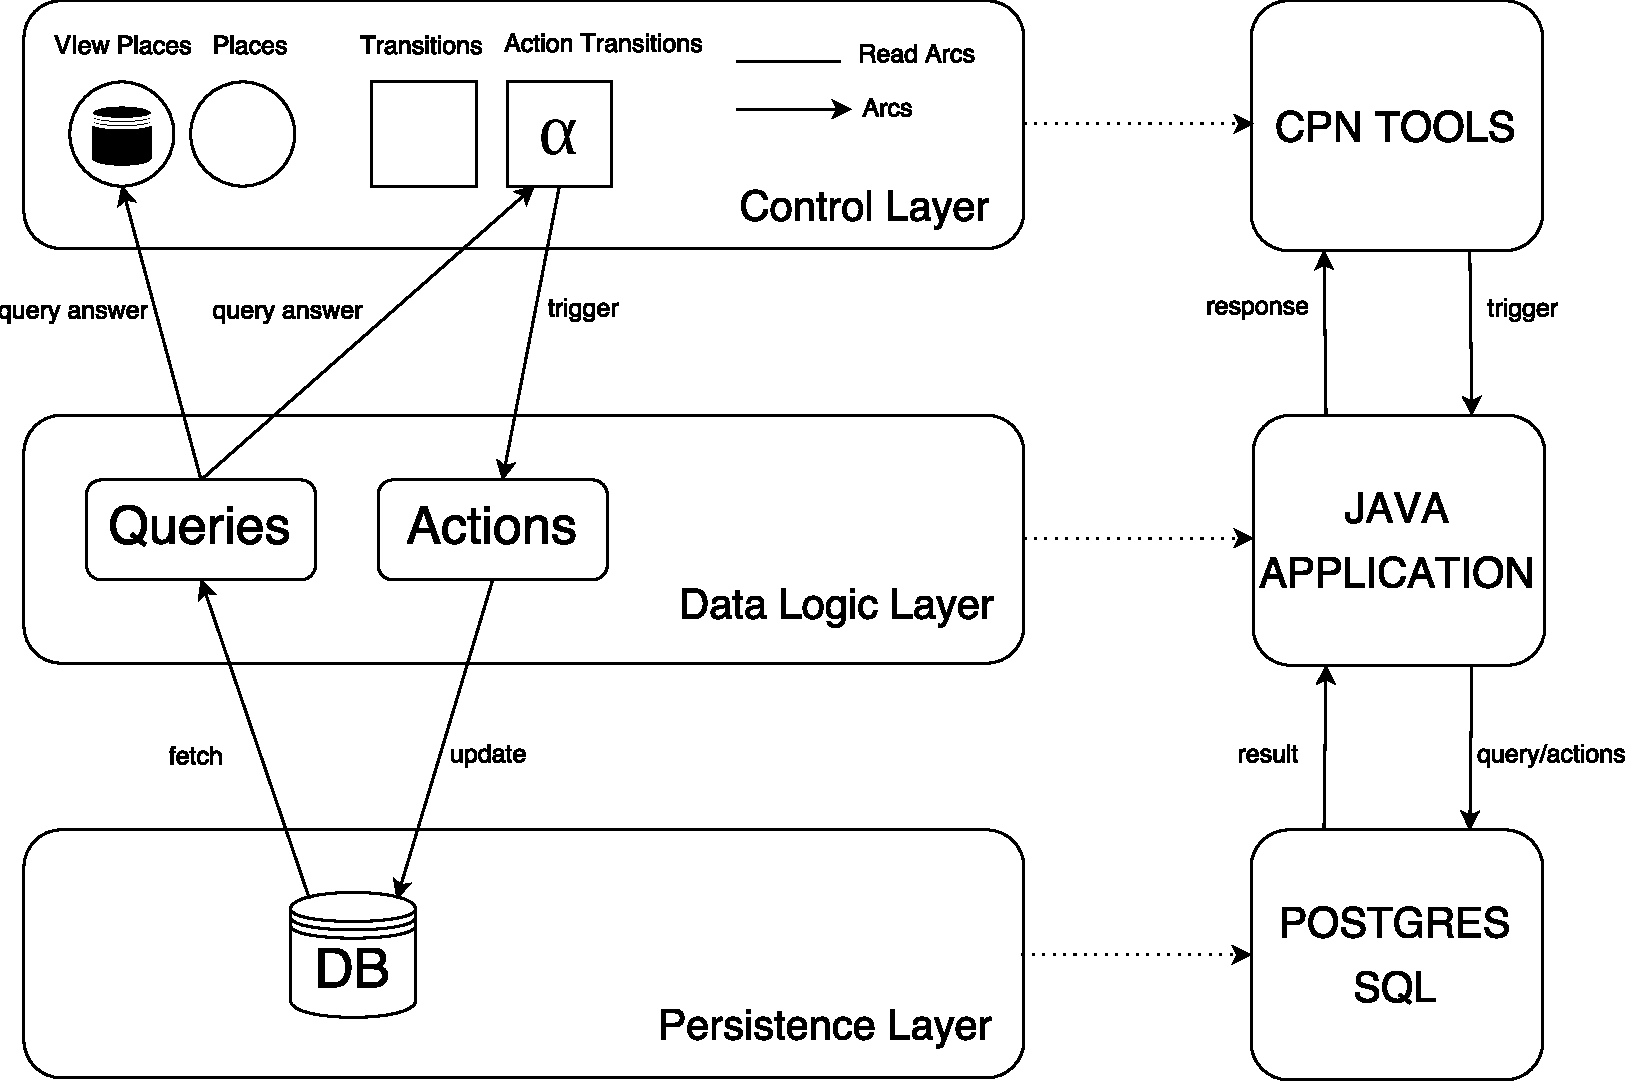
\includegraphics[scale = 0.35]{DBN_Impl_Mapping_Framework.pdf}
	\caption{The mapping of DB-net framework}
	\label{fig:DBN_Impl_Mapping_Framework}
\end{figure}

\subparagraph*{\textnormal{Figure \ref{fig:DBN_Impl_Java_App_Division} shows the framework through which the communication among different components takes place.
\begin{figure}[!htbp]
\centering
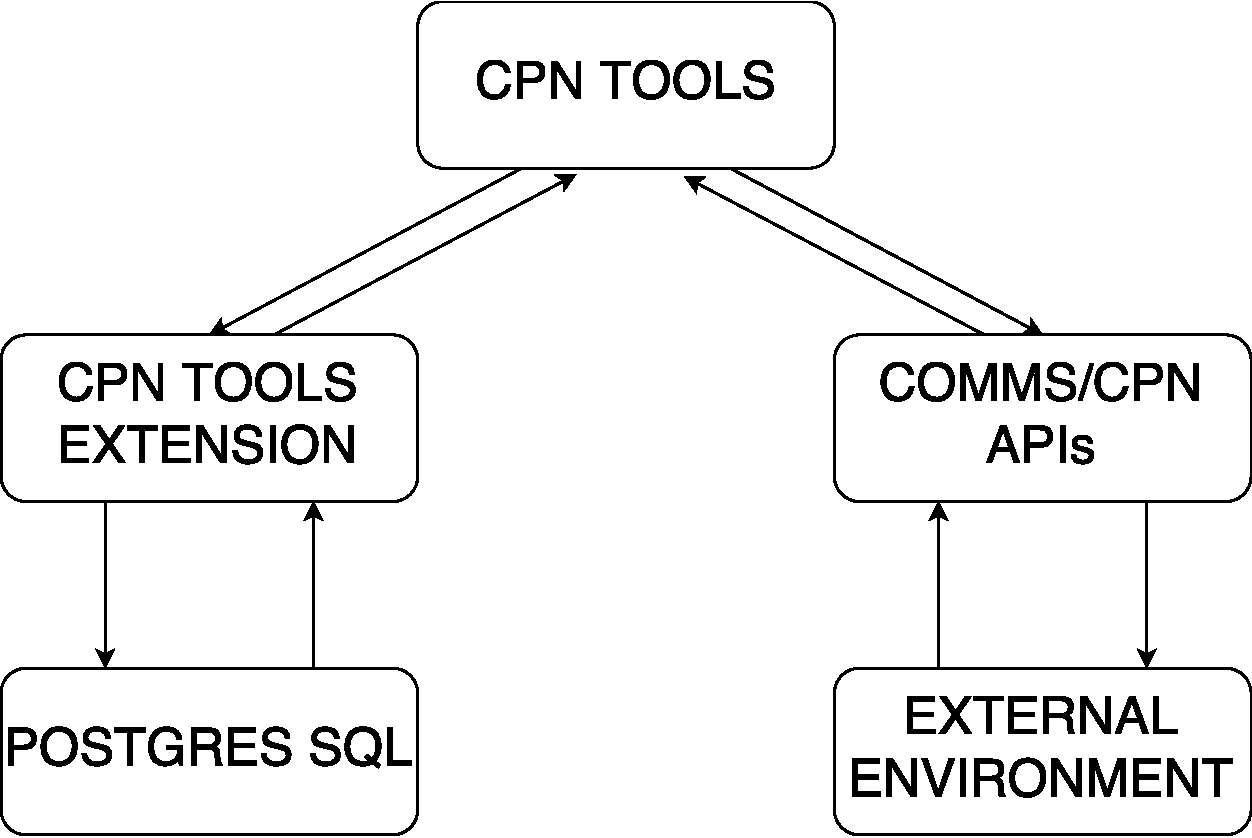
\includegraphics[scale = 0.35]{DBN_Impl_Java_App_Division.pdf}
\caption{Interconnectivity between different components}
\label{fig:DBN_Impl_Java_App_Division}
\end{figure}
Comms/CPN is used to connect to external environment/processes, which could possibly be web services etc., for data acquisition. Instead of connecting to web services, we connect to the \textit{Poll Server}.  The \textit{Poll Server} contains our JAVA functions which are used to facilitate data acquisition and executing CRUD(\textit{Create, Read, Update, Delete}) operations. The view places are populated through extension and the action transitions are executed using the \textit{Poll Server}, hence both the components are connected to the database (see Figure \ref{fig:DBN_Impl_Layer_Framework}). Connecting the \textit{Poll Server} to the database also opens up the possibility to acquire data from the database.   
\begin{figure}[!htbp]
	\centering
	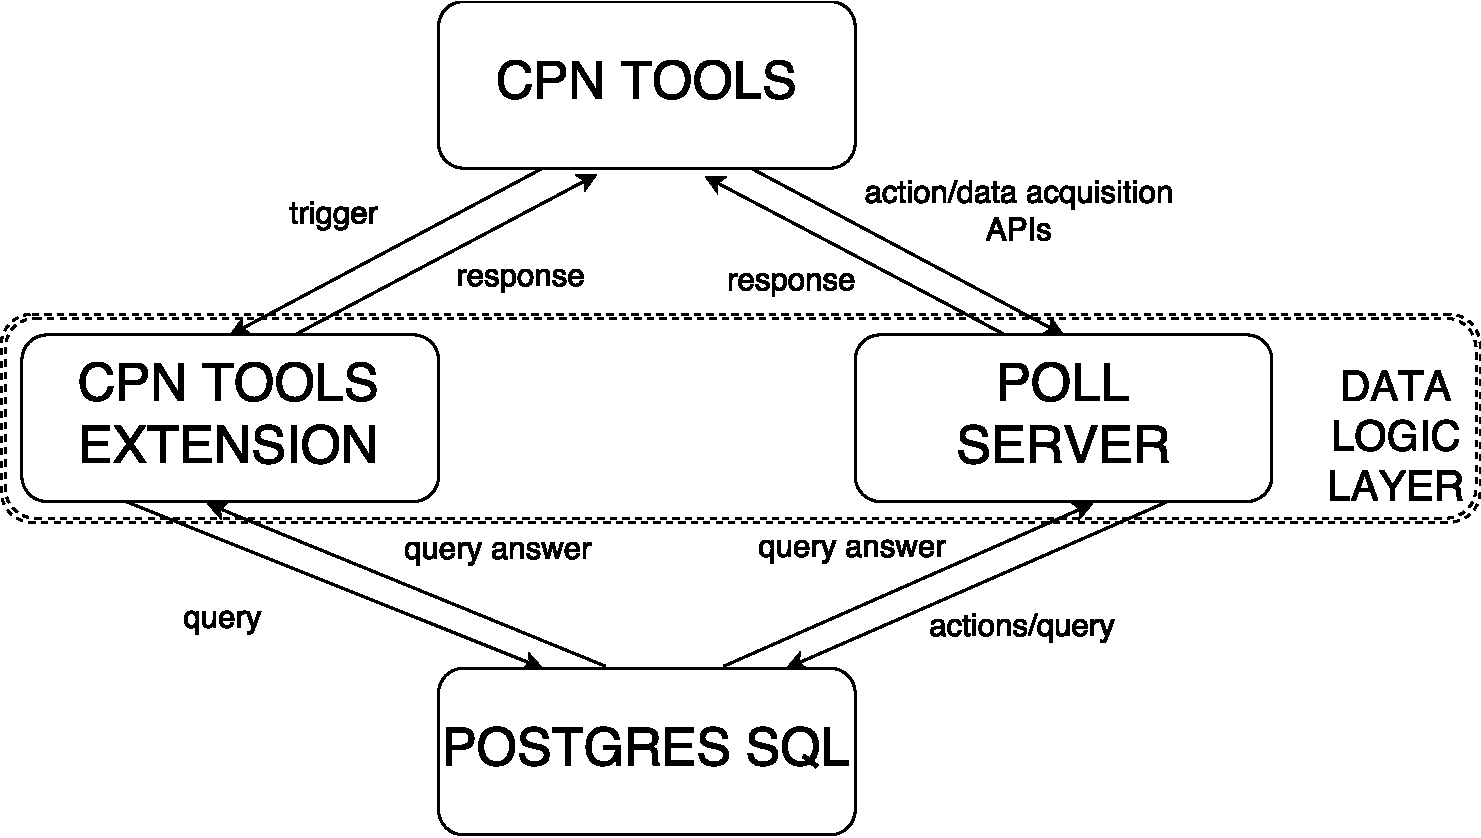
\includegraphics[scale = 0.35]{DBN_Impl_Layer_Framework.pdf}
	\caption{Data logic layer division}
	\label{fig:DBN_Impl_Layer_Framework}
\end{figure}
}}

\subsection{Persistence Layer}
\subparagraph*{\textnormal{The persistence layer consists of the database schema. We model our database schema in PostgresSQL, which allows the modelling of a full fledged relational database with constraints such as primary keys, foreign keys etc. The persistence layer is capable of returning answer to the query attached to view places along with executing actions attached to the transitions.}}

\subsection{Control Layer}
\subparagraph*{\textnormal{We use CPN Tools to implement our control layer. In CPN Tools, we define action transitions and view places which have actions and query attached to them. Let us see how to model view places and transitions in CPN Tools.}}

\subparagraph*{\textnormal{View places are drawn like normal places in CPN Tools. Also, view places carry SQL queries along themselves. Using \bsq{Text} tool one could write a statement defining the view place. Note that in the CPN model, the view places should always be connected with read arcs. The syntax\footnote{In CPN Tools, the net elements are drawn on a page which is the part of the CP net.} to define a view place is:}}
\begin{verbatim}
view_place : <PageName.PlaceName> : <SQL Query>
\end{verbatim}

\subparagraph*{\textnormal{For example, in Figure \ref{fig:DBN_Impl_Short_VP_AT_Example}, the place $\mathit{Free\ Taxi}$ has a FOL query attached. If we want to declare the place $\mathit{Free\ Taxi}$ as view place using the SQL query we could declare it as:}}

\begin{figure}[!htbp]
	\centering
	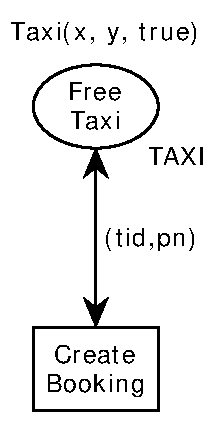
\includegraphics[scale = 0.35]{DBN_Impl_Short_VP_AT_Example.pdf}
	\caption{Example of view place}
	\label{fig:DBN_Impl_Short_VP_AT_Example}
\end{figure}

\subparagraph*{}
\begin{lstlisting}[showstringspaces=false, language = ML, caption = View place declaration example: $\mathit{Free\ Taxi}$, captionpos=b]
view_place : Booking.Free Taxi : SELECT "TID","PlateNum" FROM taxi WHERE "isFree" = TRUE;
\end{lstlisting}

\subparagraph*{\textnormal{where $\mathit{taxi}$ is the relational schema. The view place shows the details of taxis, such as taxi id and plate number, which are available for booking.}}

\subparagraph*{\textnormal{The actions attached to the transitions are modelled using ML functions. These ML functions internally use Connection Management Layer APIs provided by the Comms/CPN. As described in \cite{CPN_Tools_CodeSegment}, the code segment of transitions helps us in defining actions. The code segment has \textit{input}, \textit{output} and \textit{action} part. The input variables (the variables of interest over the incoming arc) should be mentioned in the \textit{input} part and the fresh variables, used for acquiring data, should be mentioned in the \textit{output} part. The \textit{action} part has \textit{let\ldots in \ldots end} construct which is similar to the construct of ML functions (see Listing \ref{lst:DBN_Impl_Modeling_Actions}). The fresh variables acquire data in the \textit{let} part whereas \textit{in} part contains CRUD operations. Just before the \textit{end} part, the fresh variables (if any) should be mentioned within parentheses following the order of variables in the \textit{output} part.}}

\subparagraph*{}
\begin{lstlisting}[showstringspaces=false, language = ML, caption = Code Segment: action transition, captionpos=b, label = lst:DBN_Impl_Modeling_Actions, numbers=left,
stepnumber=1]
input(<input variables>);
output(<fresh variables>);
action
let
<Data Acquisition/ Perform Actions>
in
<Perform Actions>
(<return fresh variables>)
end;
\end{lstlisting}

\subparagraph*{\textnormal{In Figure \ref{fig:DBN_Impl_Short_VP_AT_Example1}, we show the modelling of the view place $\mathit{Free\ Taxi}$ and the action transition $\mathit{Create\ Booking}$. The transition $\mathit{Create\ Booking}$ takes the free taxi and makes it unavailable for further booking. The code segment of the $\mathit{Create\ Booking}$ transition can be written as:}}

\subparagraph*{}
\begin{lstlisting}[showstringspaces=false, language = ML, caption = Code Segment: \textit{Create Booking} transition, captionpos=b, label = lst:DBN_Impl_Create_Booking_code_segment_example, numbers=left,
stepnumber=1]
input(t_id);
output();
action
let
in
RESERVE(t_id);
()
end;
\end{lstlisting}

\begin{figure}[!htbp]
	\centering
	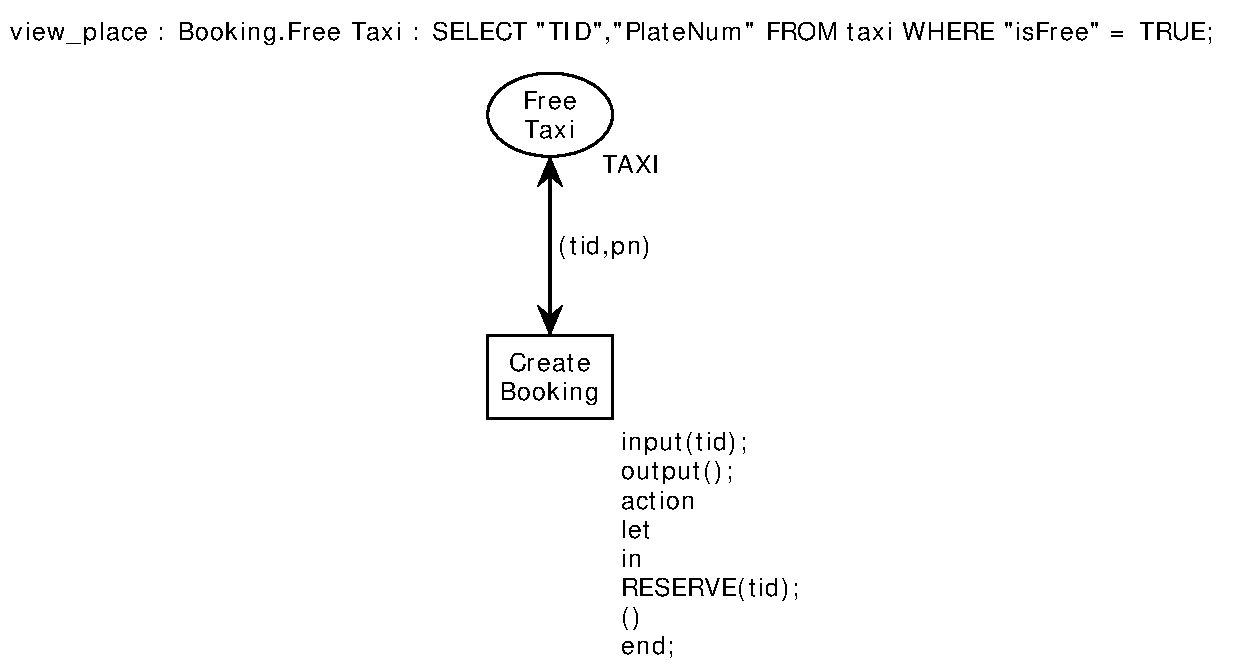
\includegraphics[scale = 0.55]{DBN_Impl_Short_VP_AT_Example_1.pdf}
	\caption{Modelling view place and action transition}
	\label{fig:DBN_Impl_Short_VP_AT_Example1}
\end{figure}

\subsection{Data Logic Layer}
\label{subsec:DBN_Impl_Implementation_Data_Logic_Layer}
\subparagraph*{\textnormal{As shown in Figure \ref{fig:DBN_Impl_Layer_Framework}, the data logic layer comprises of two parts:
\begin{itemize}
	\item A CPN Tools extension
	\item Poll Server
\end{itemize}
}}
\subsubsection*{CPN Tools extension}
\subparagraph*{\textnormal{We develop a CPN Tools extension to implement our data logic layer. With the user specified connection parameters, the extension maintains a connection with the database (Postgres SQL) using JDBC\footnote{a driver which allows JAVA application to connect to a database.} driver. The extension subscribes to CPN miscellaneous control facilities, e.g., the save event of a net, compile declarations, e.g., colour-set declaration and simulation commands, e.g., firing a transition, which are provided by CPN Tools. The main responsibilities of this extension are to:
\begin{enumerate}
\item keep track of all the net elements of the model. Also, store information about the model, such as model name, model location, pages in the net etc.
\item keep track of colour-set declarations in the CPN model. This is useful for populating the view places as we need to know the colour-set of the place before applying any marking over it.
\item keep track of the view places defined in the DB-net model, fetch the answer to the query attached to view places and calculate the markings accordingly.
\item interact with the simulator to check if the calculated markings are compatible with the colour-set the view places.
\item update the GUI on each occurring step in the simulation.
\end{enumerate}
The communication between simulator, GUI and extensions is based on packet forwarding mechanism. The communication takes place over a channel which carries the packets. Subscription to an interested event results in a notification, in form of a packet, to which we send a response. For example, once the view place is declared and the database connection is established, it results in a notification to the extension and consequently, the marking is fetched from the database and the view place is updated.}}

\subparagraph*{\textnormal{Using callback messages \cite{CPN_Tools_Callback_Messages}, one could update the GUI. In this case, a packet, including the desired update for the GUI, has to be created and passed over the channel. Note that passing invalid packets over the channel may lead CPN Tools into an inconsistent state. We design our extension on the communication pattern shown in Figure \ref{fig:DBN_Impl_Extension_Communication_Pattern}.
\begin{figure}[!htbp]
	\centering
	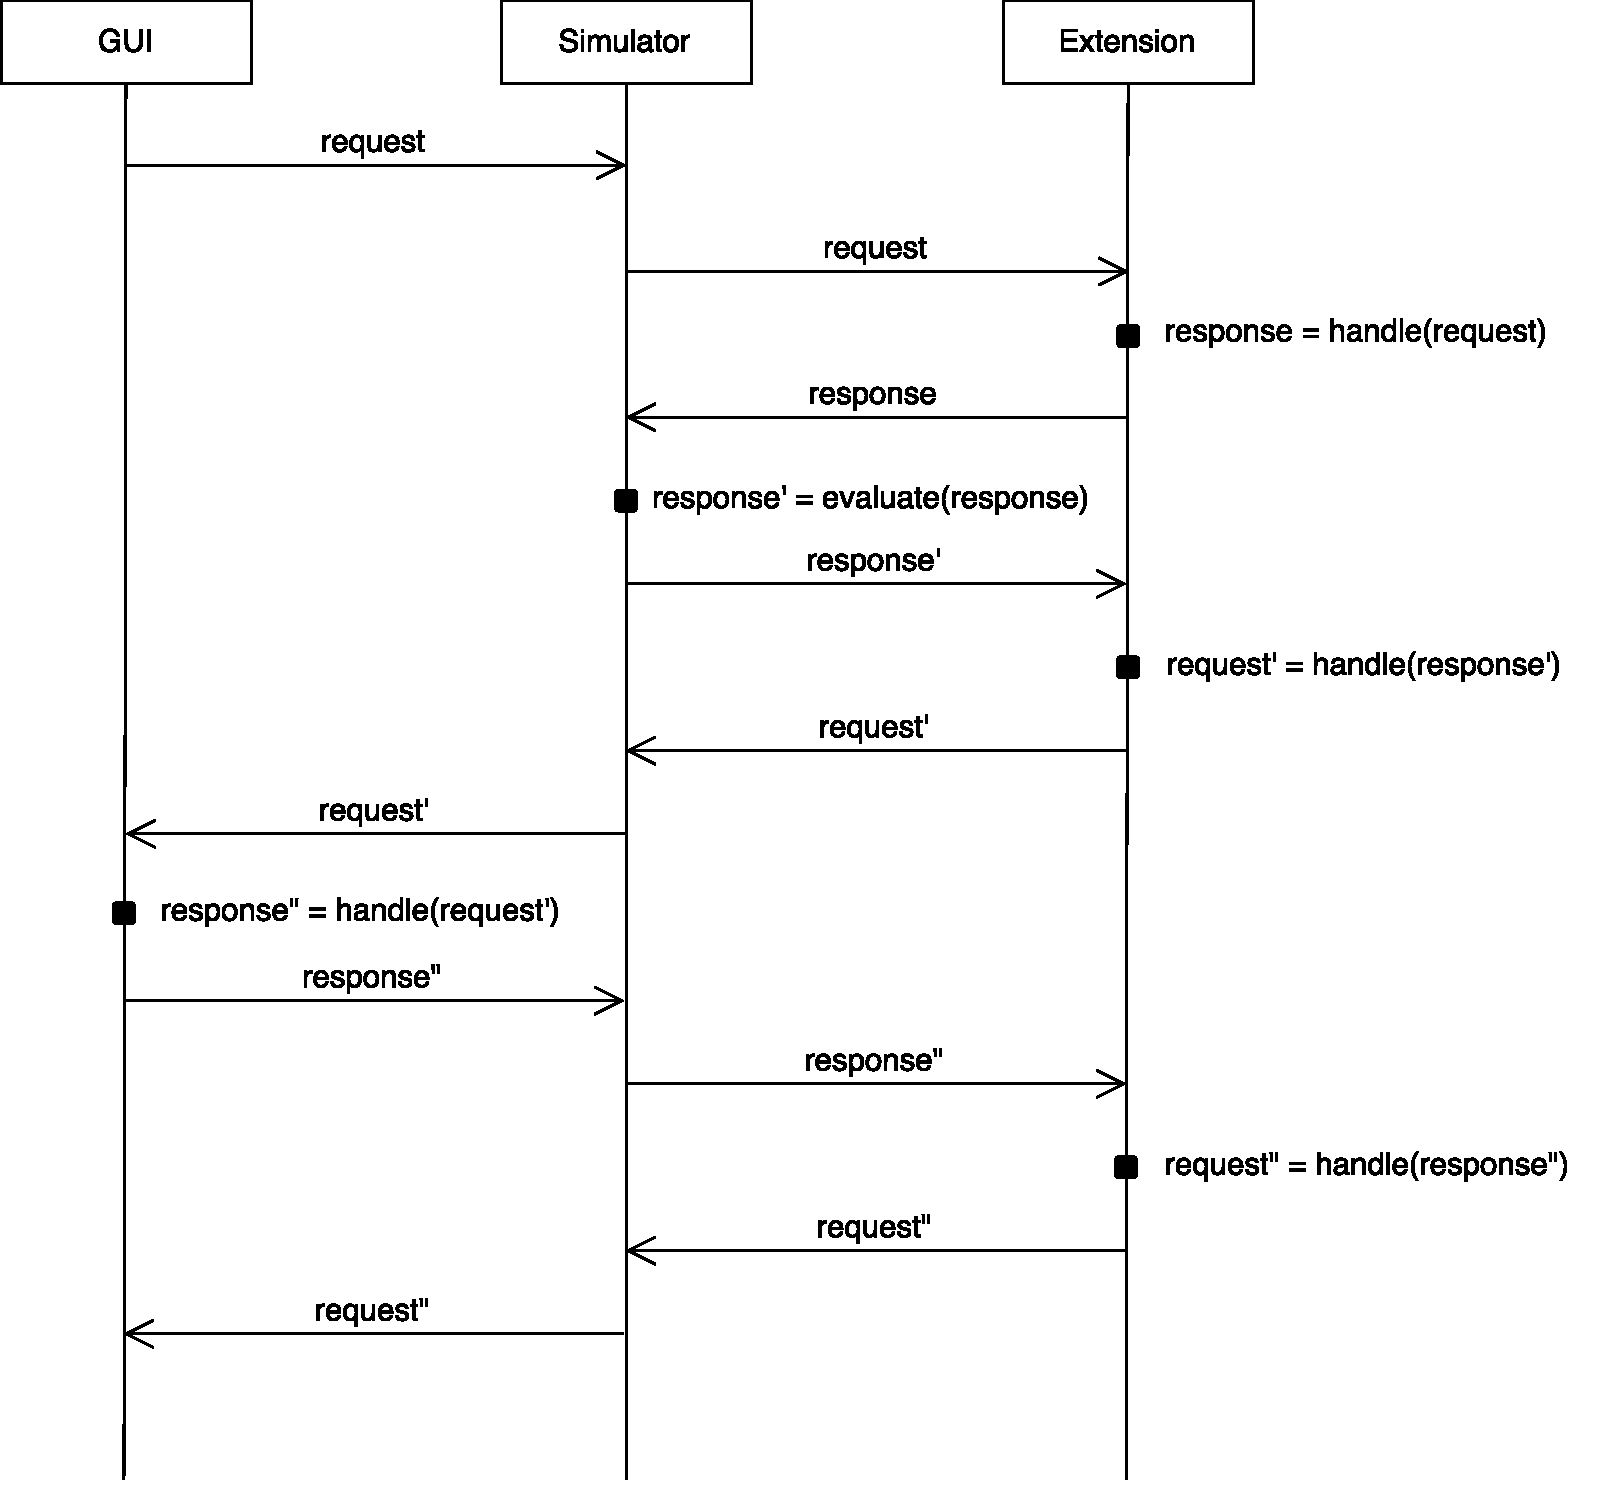
\includegraphics[scale = 0.40]{DBN_Impl_Extension_Communication_Pattern.pdf}
	\caption{Communication Pattern of CPN Tools extensions}
	\label{fig:DBN_Impl_Extension_Communication_Pattern}
\end{figure}
}}
\subparagraph*{\textnormal{In Figure \ref{fig:DBN_Impl_Extension_Communication_Pattern}, when a subscribed event occurs, the messages are passed from the GUI to the simulator over the channel. We call such messages as \textit{requests}. The extension takes appropriate response on the request and passes the response to the simulator. Simulator checks whether the response could be safely incorporated by the GUI, i.e., the response should not bring CPN Tools to an inconsistent state and returns its evaluation to the extension. Once the evaluation is received, the extension handles the evaluated response and makes a request to update the GUI. Once the request is incorporated/rejected by GUI, the corresponding response is sent to the extension. Extension handles the received response and gives the control back to the GUI.}}

\subparagraph*{\textnormal{Let us see an example of populating view places using the communication pattern presented in Figure \ref{fig:DBN_Impl_Extension_Communication_Pattern}. When we declare a view place, the extension determines the declaration by scanning the net. In this case, the \textit{request} is passed from the GUI to the extension via simulator. The extension \textit{handles} the \textit{request} and takes appropriate \textit{response} by fetching the marking (for the view place) from the database. However, at this stage, the extension does not know if the markings are compatible with the colour-set of the view place. In order to verify if the marking is compatible with the colour set of the view place, the \textit{response} is passed to the simulator. The simulator evaluates (verification of the marking) the \textit{response} and provides its decision (\textit{response\textquotesingle}) to the extension whether the marking is compatible with the colour set of the view place. Upon receiving the evaluation, extension handles it and in case the marking is compatible, it creates a new request (\textit{request\textquotesingle}) to update the marking of the view place and passes on to the GUI via simulator. On receiving the new request (\textit{request\textquotesingle}), the GUI updates the marking of the view place. After incorporating the request (by changing the marking of view place), the GUI sends a response (\textit{response\textquotedbl}) to the extension whether the request (\textit{request\textquotesingle}) was successfully incorporated or not. Upon receiving the response (\textit{response\textquotedbl}), the extension handles it and gives back the control to the GUI.}}

\subparagraph*{\textnormal{Similarly, on subscription basis, the extension receives the notification once we write any declaration, e.g., colour-set, variables etc., in CPN Tools. The extension also receives the notification when a model is loaded or saved in CPN Tools. Simulation related messages, e.g., firing of transitions, enabledness of transitions, markings of the places etc. are also subscribed. This extension is registered to CPN Tools extension server, used to boot all the registered extensions, and loaded as soon as CPN Tools is started.}}

\subsubsection*{Poll Server}
\subparagraph*{\textnormal{\textit{Poll Server} is a JAVA process which comprises of JAVA functions intended to execute actions attached to the transitions and facilitate data acquisition. The \textit{Poll Server} is connected to CPN Tools with JAVA/CPN and also connected to the database (Postgres SQL) through JDBC. The JAVA functions written in \textit{Poll Server} for facilitating data acquisition and executing actions can be called in an indirect way from CPN Tools using Comms/CPN APIs. We encapsulate the name of the JAVA functions (contained in \textit{Poll Server}) along with its parameters in a formatted string and send it through Comms/CPN. When the formatted string is received, it is parsed and the corresponding function with corresponding parameters is called. These functions can possibly have many internal APIs which can be called by passing the function API as a parameter. Currently, we provide three functions in the \textit{Poll Server} which are:
\begin{enumerate}
\item \textit{getRandom} - takes two parameters in order: \textit{funcAPI} and \textit{length}. The function API (\textit{funcAPI}) can be either \textit{randomInt}, \textit{randomString} or \textit{randomTime}. Based on the function API, data logic layer decides which function should be called and returns the result of the specified length. Currently, the function API \textit{randomTime} returns a random time in $\langle hh:mm:ss \rangle$ format which is compatible with SQL.
\item \textit{getFromDB} - takes four parameters in order: \textit{funcAPI}, \textit{tableName}, \textit{columnName} and \textit{length}. Currently, the supported function API (\textit{funcAPI}) is \textit{genUniqueID}, which generates a random unique identifier of given length for the specified \textit{tableName} and \textit{columnName}.
\item \textit{exQuery} - takes one parameter: \textit{query}. This function executes the given query.
\end{enumerate}
}}

\section{DB-nets example}
\label{sec:DBN_Impl_DBN_example}
\paragraph*{\textnormal{In this section, we will discuss the taxi booking example discussed in the previous chapter. First, we discuss our database schema and then we take the example of the CPN drawn for the taxi booking example in the previous chapters. We transform the CPN into a DB-net while explaining modelling guidelines for action transitions and view places.}}

\subparagraph*{\textnormal{We start with modelling our database schema in PostgresSQL. We name our database schema as \bdsq{taxi\_booking} (see Figure \ref{fig:DBN_Impl_Persistence_Layer}) which contains tables and constraints. The table \textit{session} contains the unique session ids generated for each booking session. The table \textit{taxi}, \textit{phone} and \textit{pickup\_data} contains information regarding taxi, customer's phone details and pickup details. \textit{booking} table stores data related to the final booking. As indicated in Figure \ref{fig:DBN_Impl_Persistence_Layer}, the database schema also contains primary key and foreign key constraints\footnote{primary keys and foreign are indicated in the schema using underlines and arrows respectively.}.}}

\begin{figure}[!htbp]
	\centering
	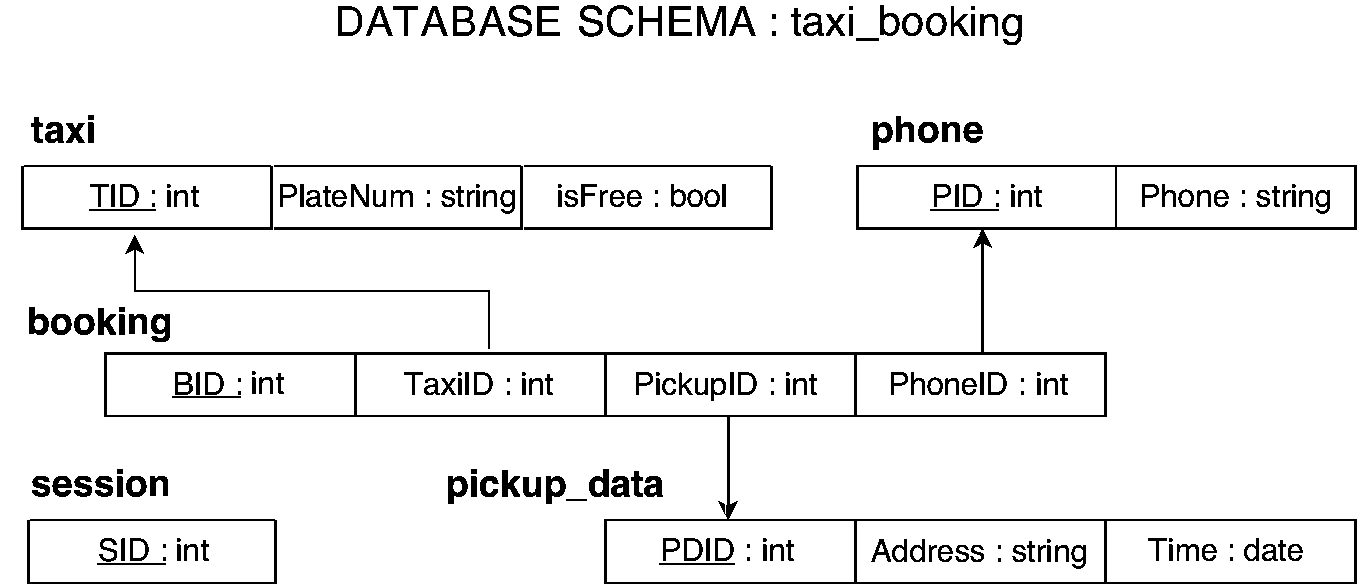
\includegraphics[scale = 0.45]{DBN_Impl_Persistence_Layer.pdf}
	\caption{Database Schema for taxi booking example}
	\label{fig:DBN_Impl_Persistence_Layer}
\end{figure}

\subparagraph*{\textnormal{In Figure \ref{fig:DBN_Impl_CPN_Taxi_Booking}, we present the CPN model of the taxi booking example presented in previous chapters. In this example, we transform the $\mathit{Free\ Taxi}$ place into a view place which would represent taxis available for booking. We also transform $\mathit{Create\ Booking}$ transition into an action transition, which will make the selected taxi unavailable for further booking. We connect $\mathit{Free\ Taxi}$ view place and $\mathit{Create\ Booking}$ transition with a read arc\footnote{The read arc is modelled as a doubled headed arc in CPN Tools.} (see Figure \ref{fig:DBN_Impl_Control_Layer}).}}

\begin{figure}[!htbp]
	\centering
	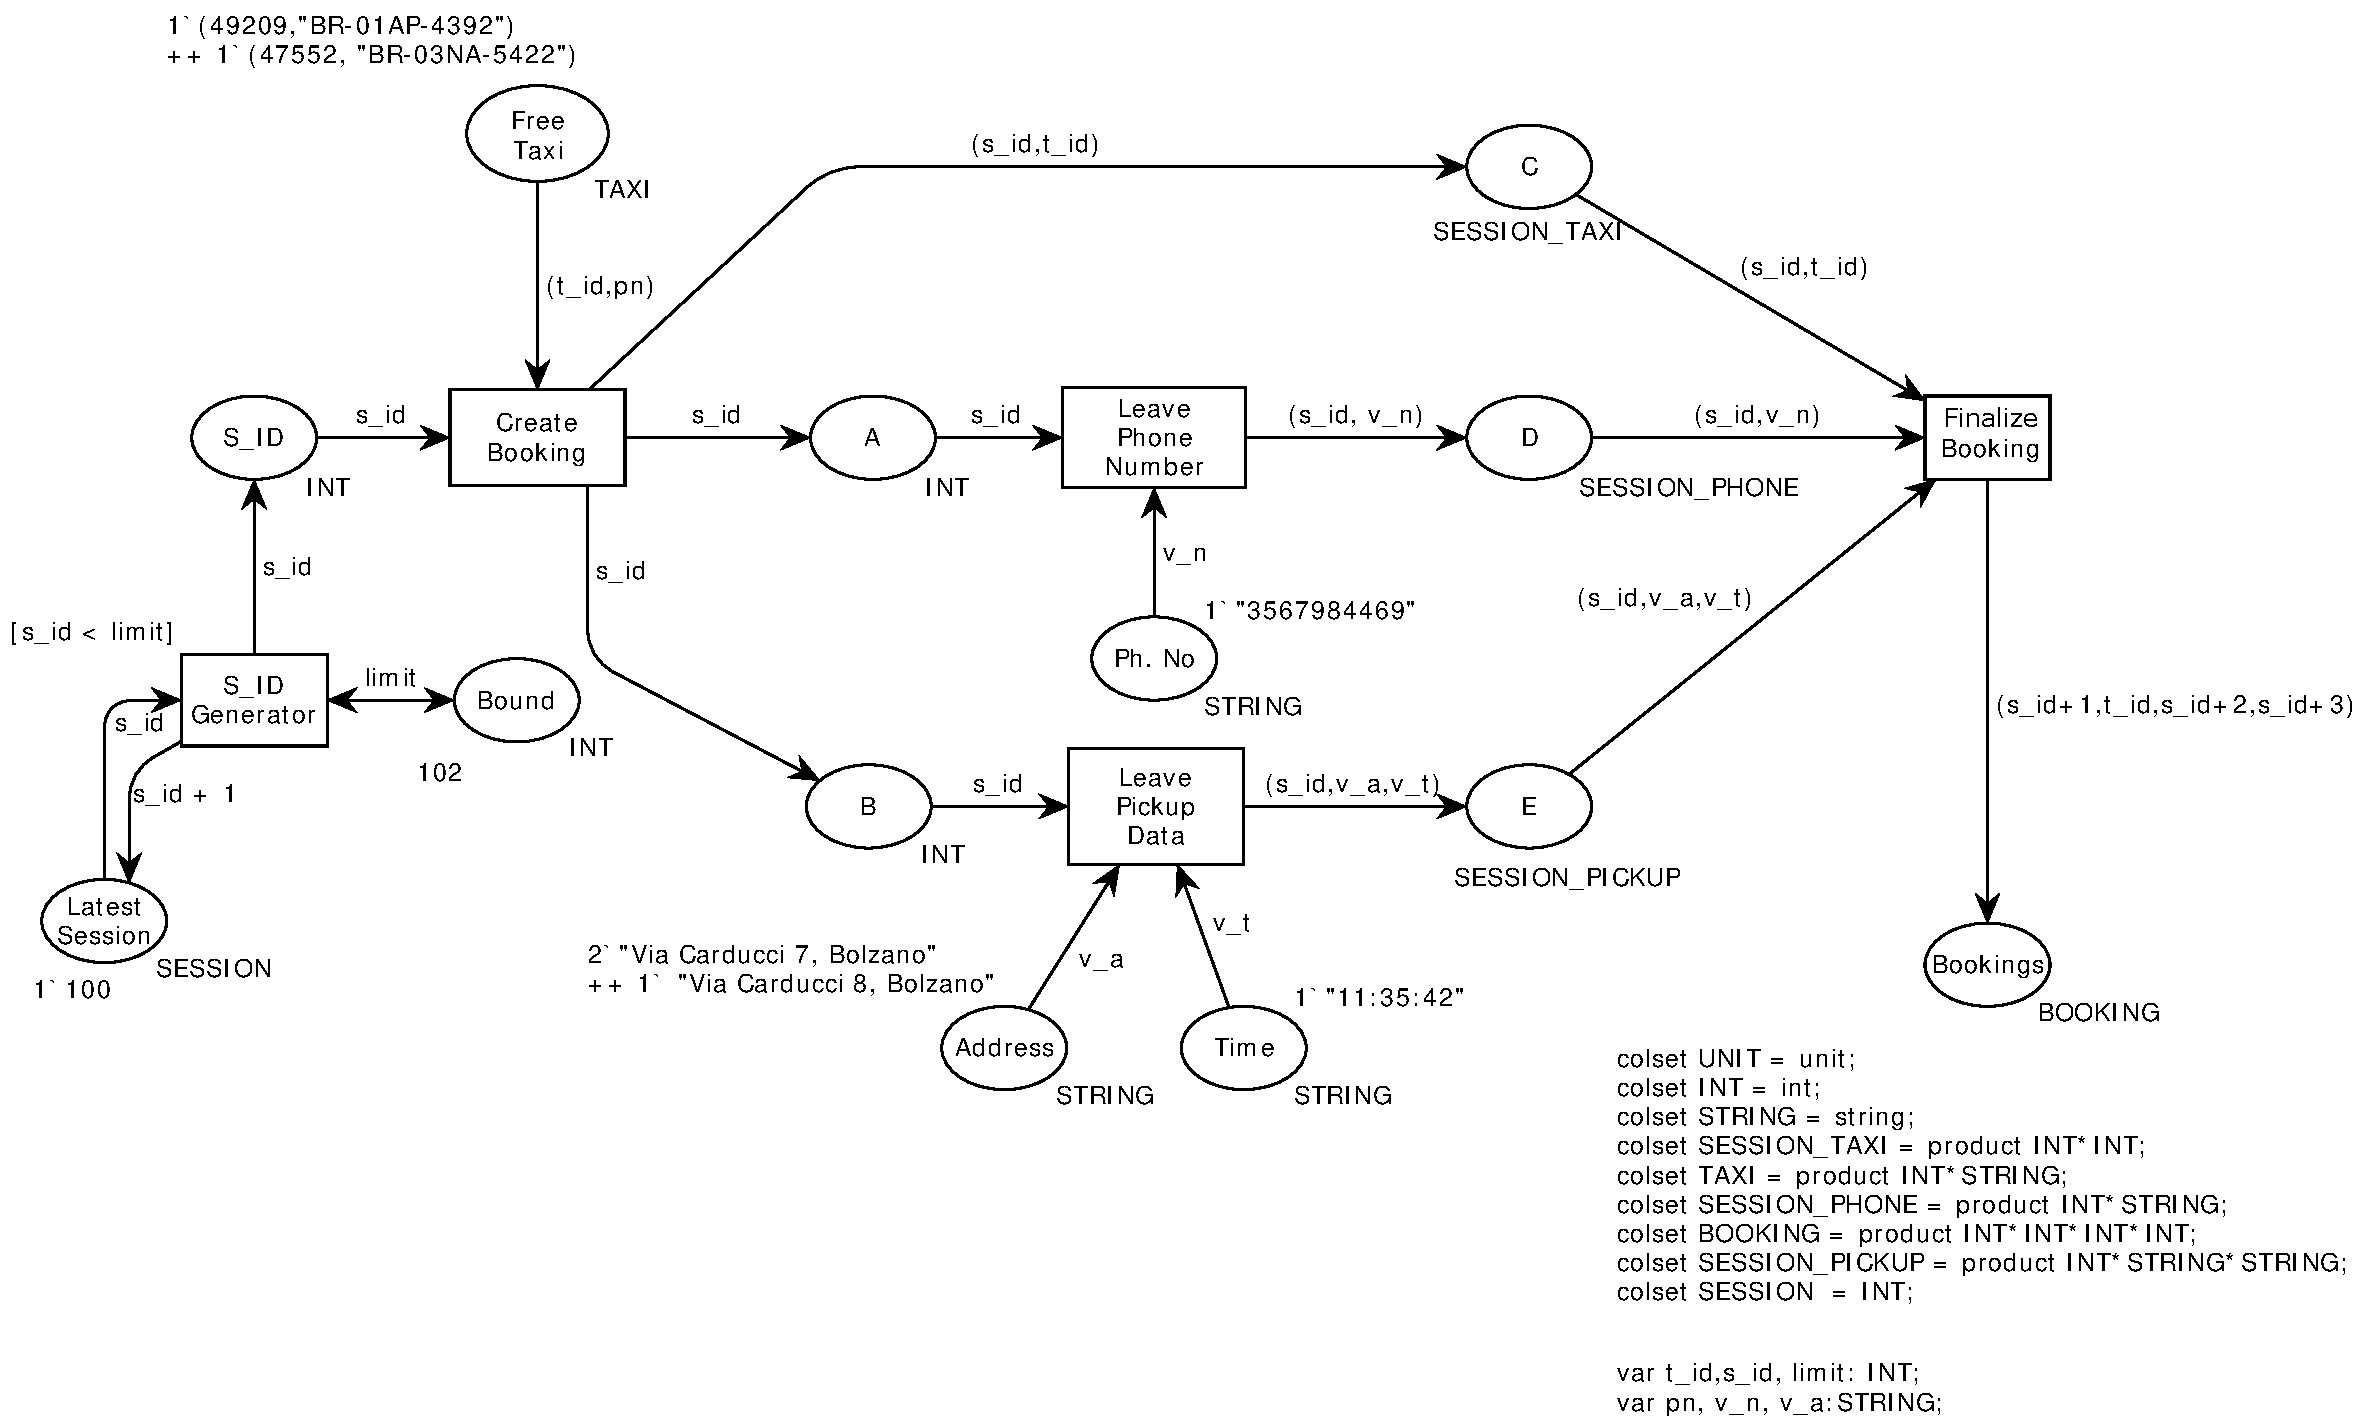
\includegraphics[scale = 0.35]{DBN_Impl_CPN_Taxi_Booking.pdf}
	\caption{CPN model for taxi booking example}
	\label{fig:DBN_Impl_CPN_Taxi_Booking}
\end{figure}

\begin{figure}[!htbp]
	\centering
	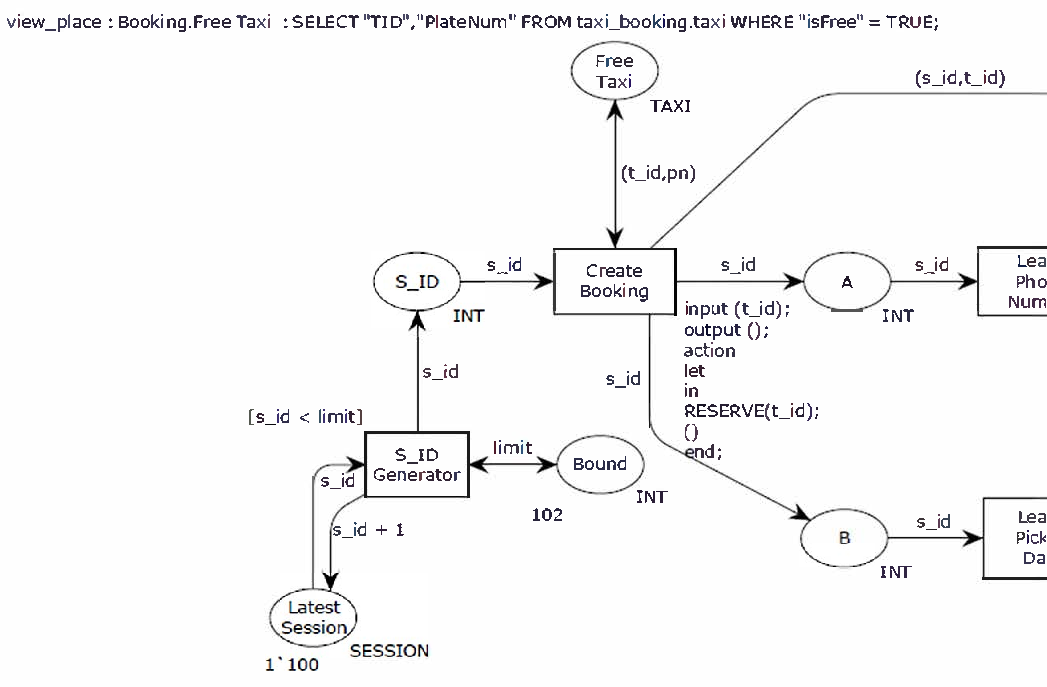
\includegraphics[scale = 0.60]{DBN_Impl_Control_Layer.pdf}
	\caption{View Place, Action Transition and Read Arcs representation}
	\label{fig:DBN_Impl_Control_Layer}
\end{figure}

\subparagraph*{\textnormal{In Figure \ref{fig:DBN_Impl_Control_Layer}, following the syntax, we define the view place using the \bsq{Text} tool and write the query attached to the view place as:}}

\subparagraph*{}
\begin{lstlisting}[showstringspaces=false, language = ML, caption = View place definition: $\mathit{Free\ Taxi}$, captionpos=b]
view_place : Booking.Free Taxi : SELECT "TID","PlateNum" FROM taxi_booking.taxi WHERE "isFree" = TRUE;
\end{lstlisting}

\subparagraph*{\textnormal{In Figure \ref{fig:DBN_Impl_Control_Layer}, the code segment of the \textit{Create Booking} transition is written as:}}

\subparagraph*{}

\begin{lstlisting}[showstringspaces=false, language = ML, caption = Code Segment: \textit{Create Booking} transition, captionpos=b, label = lst:DBN_Impl_Create_Booking_code_segment, numbers=left,
stepnumber=1]
input(t_id);
output();
action
let
in
RESERVE(t_id);
()
end;
\end{lstlisting}

\subparagraph*{\textnormal{In the code segment above, the \textit{Create Booking} transition takes a taxi id in the input part and performs an \textit{RESERVE} action related with the taxi id in the action part. The \textit{RESERVE} action is an update operation, which makes the taxi unavailable for further booking. These actions are just ML functions which we will discuss later in the chapter.}}

%\subparagraph*{\textnormal{Note that $\mathit{Create\ Booking}$ transition has a $\mathit{RESERVE}$ action attached to it. Using code segment of the transition, we could write the action part of the transition. The $\mathit{RESERVE}$ action is defined as an ML function\footnote{These ML functions are written in the declaration column in CPN Tools}:}}
%
%\subparagraph*{}
%
%\begin{lstlisting}[showstringspaces=false, language = ML, caption = RESERVE action, captionpos=b, label = lst:DBN_Impl_RESERVE_action_query]
%fun RESERVE(t_id) = exQuery("UPDATE taxi_booking.taxi SET \"isFree\" = FALSE WHERE \"TID\" ="^ Int.toString t_id^";");
%\end{lstlisting}
%
%\subparagraph*{\textnormal{\textit{exQuery} is an ML function which takes the query\footnote{In the query, (see Listing \ref{lst:DBN_Impl_RESERVE_action_query}), the {\textbackslash \textquotedbl} symbol is used in ML to represent double quotes in string where as $\string^$ symbol is used to concatenate two strings.} as a parameter and passes it to Comms/CPN for execution.}}

\subparagraph*{\textnormal{$\mathit{Leave\ Phone\ Number}$ and $\mathit{Leave\ Pickup\ Data}$ transitions are also transformed into action transition. These transitions carry fresh variables which are used for acquiring data from the environment. We remove the places $\mathit{Ph. No}$, $\mathit{Address}$ and $\mathit{Time}$ (see Figure \ref{fig:DBN_Impl_CPN_Taxi_Booking}), and acquire data in the code segment of \textit{Leave Phone Number} and $\mathit{Leave\ Pickup\ Data}$ transitions (see Figure \ref{fig:DBN_Impl_Data_Acquisition}).}}

\begin{figure}[!htbp]
	\centering
	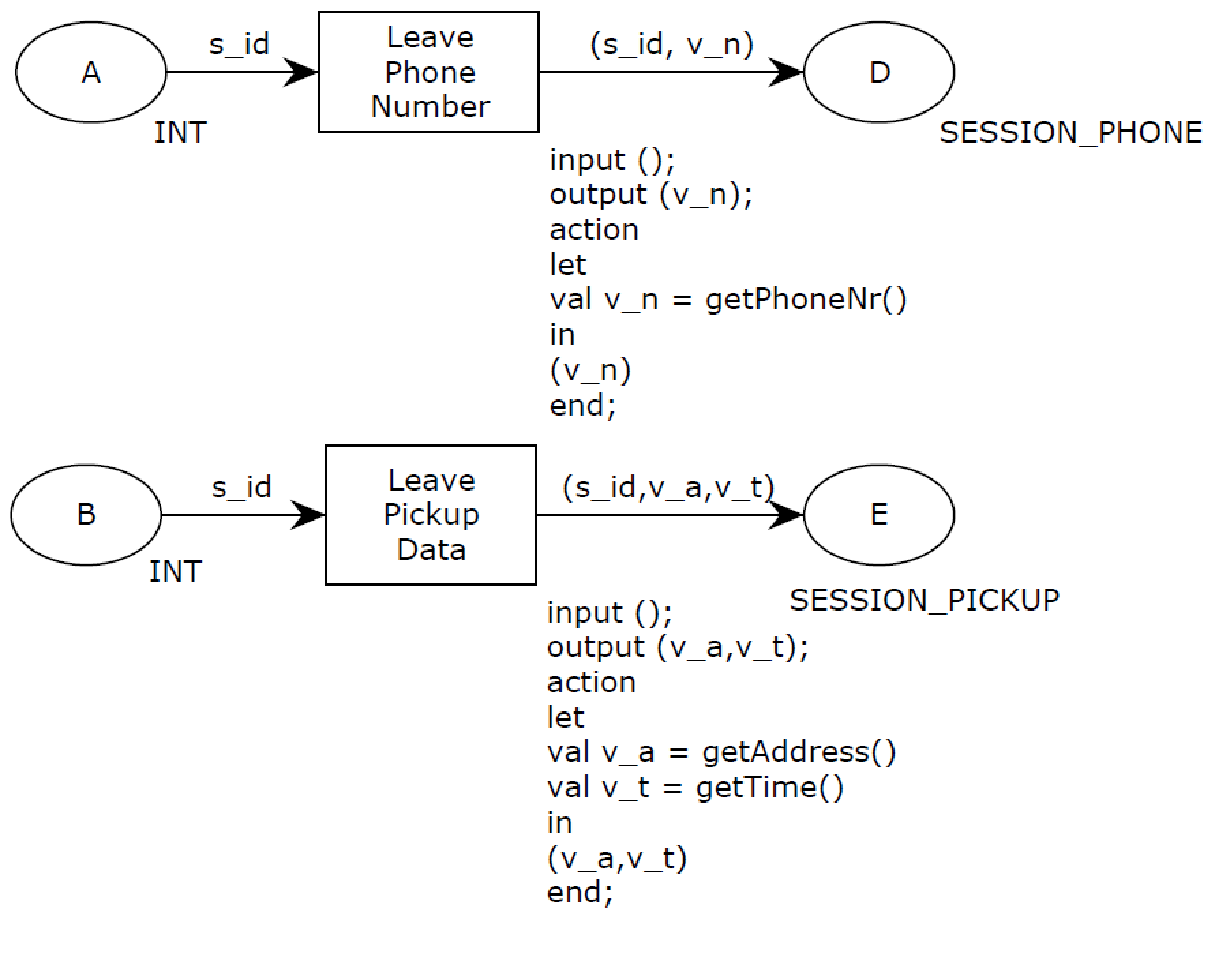
\includegraphics[scale = 0.35]{DBN_Impl_Data_Acquisition.pdf}
	\caption{Action transitions: Leave Phone Number and Leave Pickup Data}
	\label{fig:DBN_Impl_Data_Acquisition}
\end{figure}

\subparagraph*{\textnormal{The code segment of \textit{Leave Phone Number} transition is shown in Listing \ref{lst:DBN_Impl_code_segment_leave_ph_number} and the one of $\mathit{Leave\ Pickup\ Address}$ is shown in Listing \ref{lst:DBN_Impl_code_segment_leave_picup_data}. In the \textit{Leave Phone Number} transition, the fresh variable $\mathit{v\_n}$ acquires the phone number from the ML function $\mathit{getPhoneNr}$. Similarly, in the $\mathit{Leave\ Pickup\ Data}$ transition, the variables $\mathit{v\_a}$ and $\mathit{v\_t}$ acquire pickup address and time from the ML functions $\mathit{getAddress}$ and $\mathit{getTime}$ respectively. Hence, instead of providing the data before hand (as marking on places $\mathit{Ph. No}$, $\mathit{Address}$ and $\mathit{Time}$), we acquire data dynamically from the external environment.}}
\subparagraph*{}
\begin{lstlisting}[showstringspaces=false, language = ML, caption = Code segment of transition: $\mathit{LEAVE\ PHONE\ NUMBER}$, captionpos=b, label = lst:DBN_Impl_code_segment_leave_ph_number, numbers=left,
stepnumber=1]
input()
output(v_n)
let
val v_n = getPhoneNr()
in
(v_n)
end;
\end{lstlisting}

\subparagraph*{}
\begin{lstlisting}[showstringspaces=false, language = ML, caption = Code segment of transition: $\mathit{LEAVE\ PICKUP\ DATA}$, captionpos=b, label = lst:DBN_Impl_code_segment_leave_picup_data, numbers=left,
stepnumber=1]
input();
output(v_a,v_t);
action
let
val v_a = getAddress()
val v_t = getTime()
in
(v_a,v_t)
end;
\end{lstlisting}

\subparagraph*{\textnormal{In the CPN model (Figure \ref{fig:DBN_Impl_CPN_Taxi_Booking}), the transition $\mathit{S\_ID\ Generator}$ generates two session id in the range [100,101], however, it is not guaranteed that these generated session ids are unique to our relational schema \textit{session}. In order to make it unique to the session table, we transform this transition into an action transition, and using a fresh variable $\mathit{s\_id}$ we acquire a unique identifier by consulting the \textit{session} table. The transformation for the part of session id generation is shown in Figure \ref{fig:DBN_Impl_SID_Generator}. Note that, the number of session ids which can be generated is no more bounded. One could create the upper bound by introducing the $\mathit{Bound}$ place and the guard over the transition.}}

\begin{figure}[!htbp]
	\centering
	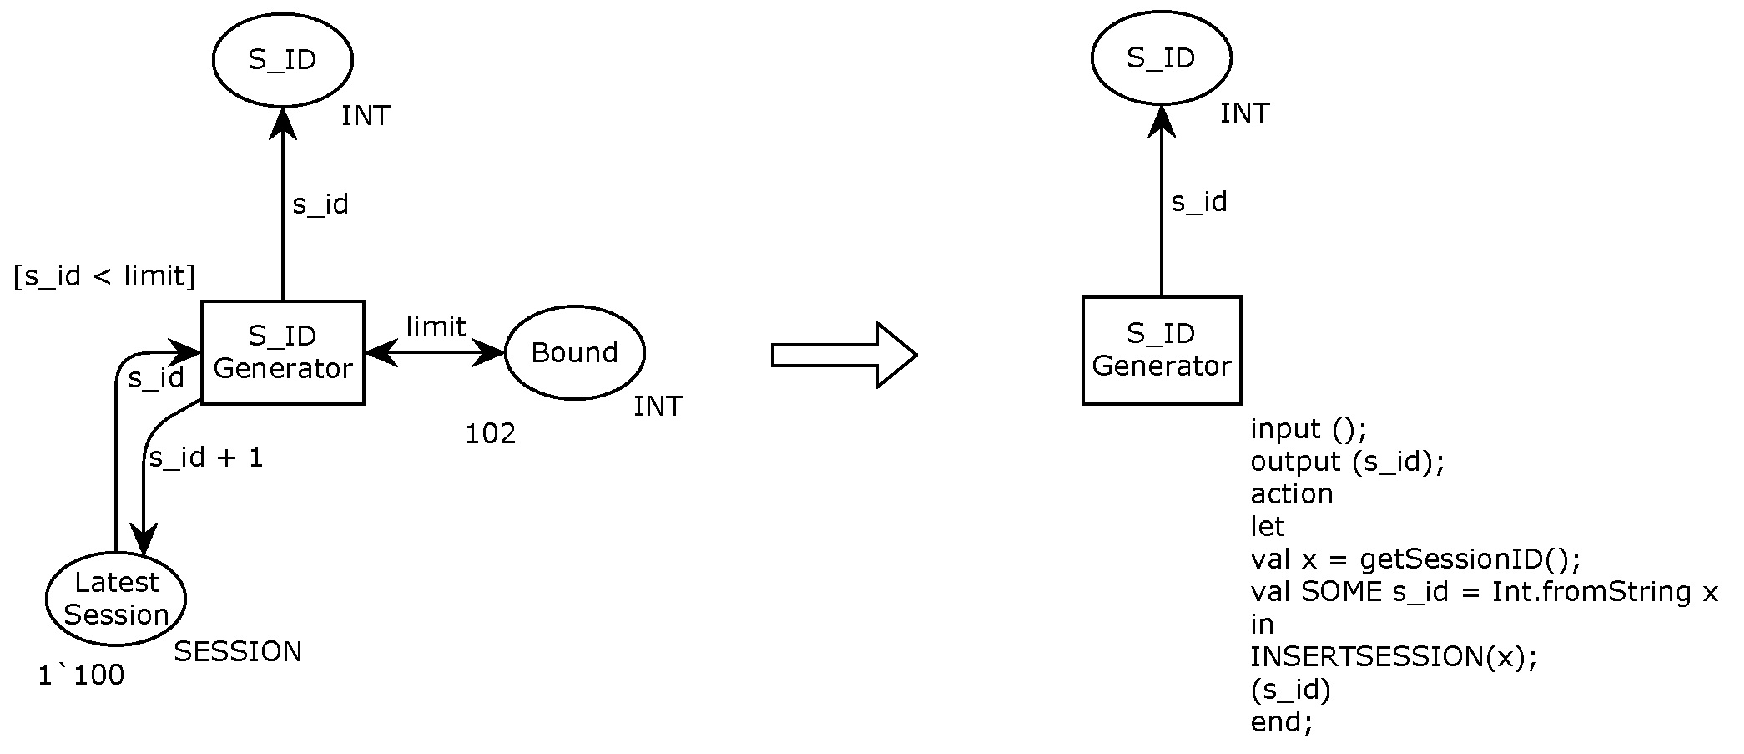
\includegraphics[scale = 0.35]{DBN_Impl_SID_Generator.pdf}
	\caption{S\_ID Generator}
	\label{fig:DBN_Impl_SID_Generator}
\end{figure}

\subparagraph*{\textnormal{The code segment of the transition $\mathit{S\_ID\ Genearator}$ is shown in Listing \ref{lst:DBN_Impl_code_segment_sid_gen}. At line 5, the ML function $\mathit{getSessionID}$ internally use Comms/CPN API and returns a unique session identifier in string format. Since the place $\mathit{S\_ID}$ has the colour-set $\mathit{INT}$, the identifier is converted to the $\mathit{INT}$ type (line number 6). In order to restrict the system from generating the same session id again, the generated session id is inserted in the \textit{session} table (line number 8) using an ML function $\mathit{INSERTSESSION}$ which internally use Comms/CPN APIs. In the end, the unique session id is generated and can be used for booking purpose.}}

\subparagraph*{}
\begin{lstlisting}[showstringspaces=false, language = ML, caption = code segment of transition : $\mathit{S\_ID\ Generator}$, captionpos=b, label = lst:DBN_Impl_code_segment_sid_gen, numbers=left,
stepnumber=1]
input();
output(s_id);
action
let
val x = getSessionID();
val SOME s_id = Int.fromString x 
in
INSERTSESSION(x);
(s_id)
end;
\end{lstlisting}

\subparagraph*{\textnormal{Similarly, we could transform $\mathit{Finalize\ Booking}$ transition as shown in Figure \ref{fig:DBN_Impl_Finalize_Booking} where $\mathit{b\_id}$, $\mathit{pd\_id}$ and $\mathit{ph\_id}$ are of \textit{INT} data type and represent booking id, pickup id and phone id respectively. The booking id, pickup id and the phone id are generated by consulting the respective tables and sequentially inserted. The code segment of $\mathit{Finalize\ Booking}$ transition is given in Listing \ref{lst:DBN_Impl_code_segment_add_booking} where $\mathit{getBookingID}$, $\mathit{getPickupID}$ and $\mathit{getPhoneID}$ are ML functions which fetch a unique id for the respective tables. $\mathit{INSERTPHONE}$, $\mathit{INSERTPICKUP}$ and $\mathit{ADDBOOKING}$ functions insert records in the corresponding relational database. Note that the order of insertion of these records matters due to the presence of the foreign key constraints. For example, the foreign key between $\mathit{booking}$ table and $\mathit{pickup\_data}$ table, allows insertion of a tuple, in $\mathit{booking}$ table, containing pickup id only when the corresponding pickup id is present in the $\mathit{pickup\_data}$ table. Similarly, one cannot remove a tuple from the $\mathit{pickup\_data}$ table if the corresponding $\mathit{pickup_id}$ is referenced in the $\mathit{booking}$ table.}}

\begin{figure}[!htbp]
	\centering
	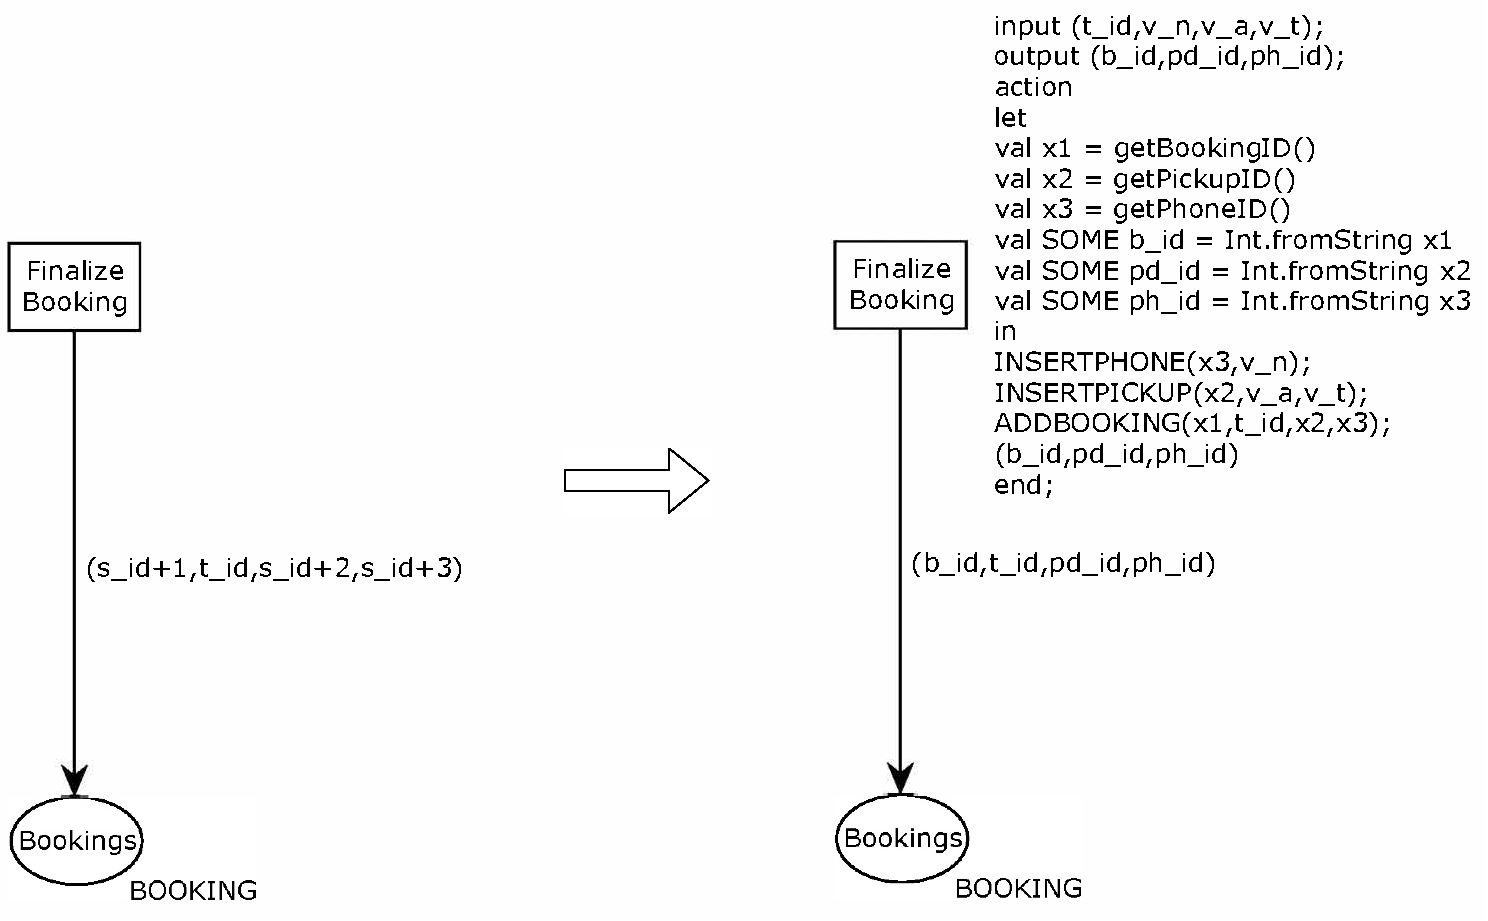
\includegraphics[scale = 0.35]{DBN_Impl_Finalize_Booking.pdf}
	\caption{$\mathit{Add\ Booking}$ transition}
	\label{fig:DBN_Impl_Finalize_Booking}
\end{figure}

\subparagraph*{}
\begin{lstlisting}[showstringspaces=false, language = ML, caption = code segment of transition : $\mathit{Finalize\ Booking}$, captionpos=b, label = lst:DBN_Impl_code_segment_add_booking, numbers=left,
stepnumber=1]
input(t_id,v_n,v_a,v_t);
output(b_id,pd_id,ph_id);
action
let
val x1 = getBookingID()
val x2 = getPickupID()
val x3 = getPhoneID()
val SOME b_id = Int.fromString x1
val SOME pd_id = Int.fromString x2
val SOME ph_id = Int.fromString x3
in
INSERTPHONE(x3,v_n);
INSERTPICKUP(x2,v_a,v_t);
ADDBOOKING(x1,t_id,x2,x3);
(b_id,pd_id,ph_id)
end;
\end{lstlisting}

\subparagraph*{\textnormal{We provide three ML functions which internally call Comms/CPN APIs and are able to communicate using the unique connection name. Users are encouraged to use these ML functions in order to interact with the database. One can also write their own ML functions and use them in a similar way. For example, one of the three ML function which we provide, $\mathit{exQuery}$ can be written as:}}

\subparagraph*{}
\begin{lstlisting}[showstringspaces=false, language = ML, caption = exQuery function, captionpos=b, label = lst:DBN_Impl_exQuery]
fun exQuery(connectionName, query) = ConnManagementLayer.send(connectionName, "exQuery"^"?"^query, stringEncode);
\end{lstlisting}

\subparagraph*{\textnormal{In the above function, the $\string^$ symbol is used to concatenate two strings in ML. The \bdsq{?} sign separates part of the string and is used to provide a marker to the parser in the \textit{Poll Server} to identify different parts of the string received from Comms/CPN. The $\mathit{exQuery}$ function takes the connection name as the first parameter, followed by the function name to be called\footnote{Here \bdsq{exQuery} is the function name in the \textit{Poll Server}.} in the \textit{Poll Server} and the query to be executed.}}

\subparagraph*{\textnormal{Let us consider an example for executing a query using the $\mathit{exQuery}$ function. The $\mathit{RESERVE}$ action mentioned in the code segment of $\mathit{Create\ Booking}$ (see Listing \ref{lst:DBN_Impl_Create_Booking_code_segment}) transition can be written as an ML function:}}

\subparagraph*{title}
\begin{lstlisting}[showstringspaces=false, language = ML, caption = RESERVE action, captionpos=b, label = lst:DBN_Impl_RESERVE_action_query]
fun RESERVE(t_id) = exQuery("Taxi_Connection","UPDATE taxi_booking.taxi SET \"isFree\" = FALSE WHERE \"TID\" ="^ Int.toString t_id^";");
\end{lstlisting}

\subparagraph*{\textnormal{In Listing \ref{lst:DBN_Impl_RESERVE_action_query} \footnote{In ML, the {\textbackslash \textquotedbl} symbol is used to represent double quotes in strings.}, we specify the connection name as $\mathit{Taxi\_Connection}$, followed by the query to be executed. As the first parameter, we specify the connection name as $\mathit{Taxi\_Connection}$, which will be used throughout our example. The query (in the \textit{RESERVE} function) updates the $\mathit{taxi}$ table and makes the selected taxi unavailable for booking. For example, for $\mathit{t\_id = 47552}$, the query passed would be :}}

\subparagraph*{}
\begin{lstlisting}[showstringspaces=false, language = SQL, caption = RESERVE action: query example, captionpos=b, label = lst:DBN_Impl_RESERVE_action_query_ex]
UPDATE taxi_booking.taxi SET "isFree" = FALSE WHERE "TID" = 47552;
\end{lstlisting}

\subparagraph*{\textnormal{The other two functions which we provide are $\mathit{getFromDB}$ and $\mathit{getRandom}$ which can be written as:}}

\subparagraph*{}
\begin{lstlisting}[showstringspaces=false, language = ML, caption = \textit{getRandom} and \textit{getFromDB} function, captionpos=b, label = lst:DBN_Impl_provided_APIs, numbers=left,
stepnumber=1]
fun getFromDB(connectionName, funcAPI, t_name, c_name, length) = (ConnManagementLayer.send(connectionName, "getFromDB"^"?"^t_name^"?"^c_name^"?"^funcAPI^"?"^length, stringEncode); ConnManagementLayer.receive(connectionName, stringDecode));
fun getRandom(connectionName, funcAPI, length) = (ConnManagementLayer.send(connectionName, "getRandom"^"?"^funcAPI^"?"^length, stringEncode); ConnManagementLayer.receive(connectionName, stringDecode));
\end{lstlisting}

\subparagraph*{\textnormal{In a similar manner as \textit{exQuery}, while sending data, \textit{getFromDB} and \textit{getRandom} encapsulate the function name which needs to be called by the \textit{Poll Server}. Following the function name, the function APIs are specified, i.e., the different flavours of the function which are offered. For $\mathit{getFromDB}$ function, currently, the supported API is only \textit{genUniqueID}. For \textit{getRandom} function, the supported APIs are \textit{getRandomInt}, \textit{getRandomString} and \textit{getRandomTime}. We use these functions (mentioned in Listing \ref{lst:DBN_Impl_provided_APIs}) for data acquisition.}}

\subparagraph*{\textnormal{In order to complete the modelling phase in CPN Tools, we have to explicitly define the ML functions called in the code segment of each transition\footnote{We assume that the user is familiar with the declaration of colour-set and variables.}(if any). The function $\mathit{getSessionID}$ and $\mathit{INSERTSESSION}$, mentioned in the code segment of $\mathit{S\_ID\ Generator}$ transition, can be defined as:}}

\subparagraph*{}
\begin{lstlisting}[showstringspaces=false, language = ML, caption = Functions for generating and inserting session ID, captionpos=b, label = lst:DBN_Impl_functions_SID_Gen,numbers=left,
stepnumber=1]
fun getSessionID() = getFromDB("Taxi_Connection","genUniqueID","taxi_booking.session","\"SID\"","6");
fun INSERTSESSION(s_id) = exQuery("Taxi_Connection","INSERT INTO taxi_booking.session VALUES ("^ s_id ^ ");" );
\end{lstlisting}

\subparagraph*{\textnormal{In the function $\mathit{getSessionID}$, we pass the first parameter as the connection name, the second parameter is the function API which needs to be called. $\mathit{taxi\_booking.session}$ is the session table in the $\mathit{taxi\_booking}$ schema which is passed as the third parameter, followed by the column name for which the unique id is to be generated, and finally, we pass the length of the desired identifier. In our case, we generate a 6 digit unique random identifier. The definition of the function $\mathit{INSERTSESSION}$ is similar to the \textit{RESERVE} function as it internally uses the $\mathit{exQuery}$ function. However, the query in the $\mathit{INSERTSESSION}$ function performs insertion in the $\mathit{session}$ table.}}

\subparagraph*{\textnormal{Similarly, one could write ML functions in the code segment of \textit{Finalize Booking} transition. The ML functions $\mathit{getBookingID}$, $\mathit{getPickupID}$ and $\mathit{getPhoneID}$ could be modelled similar to the function $\mathit{getSessionID}$, and \textit{INSERTPHONE}, \textit{INSERTPICKUP} and \textit{ADDBOOKING} could be modelled similar to $\mathit{getSessionID}$ functions. Transitions such as \textit{Leave Phone Number} and \textit{Leave Pickup Data} use ML functions \textit{getPhoneNr}, \textit{getAddress} and \textit{getTime} function to acquire a random phone number, random address and random time. These functions could be written as:}}

\subparagraph*{}
\begin{lstlisting}[showstringspaces=false, language = ML, caption = {Functions for acquiring random phone number, random address and random time}, captionpos=b, label = lst:DBN_Impl_Leave_Phone,numbers=left,
stepnumber=1]
fun getPhoneNr()=getRandom("Taxi_Connection","randomInt","10");
fun getAddress()=getRandom("Taxi_Connection","randomString","20");
fun getTime()=getRandom("Taxi_Connection","randomTime","6");
\end{lstlisting}

\subparagraph*{\textnormal{As mentioned earlier, the \textit{getRandom} function provides three different inputs based on predefined modes, \textit{randomInt}, \textit{randomString} and \textit{randomTime}. For example, the function \textit{getPhoneNr} returns a phone number (of string type) of length 10. Similarly, \textit{getAddress} function returns a random address which is a combination of 20 characters and \textit{getTime} function returns a time in $\langle hh:mm:ss \rangle$ format\footnote{This format is compatible with SQL. The length in the $\mathit{getTime}$ function is fixed right now.}.}}

\subparagraph*{\textnormal{In order to connect to a TCP/IP port, we also specify functions namely \textit{connectDB} and \textit{disconnectDB} which internally use Comms/CPN APIs and connect to the specified TCP/IP port. These functions are declared as:}}

\subparagraph*{}
\begin{lstlisting}[showstringspaces=false, language = ML, caption = {Functions for acquiring random phone number, random address and random time}, captionpos=b, label = lst:DBN_Impl_Connect_Disconnect,numbers=left,
stepnumber=1]
fun connectDB(connectionName, port) = ConnManagementLayer.acceptConnection(connectionName, port);
fun disconnectDB(connectionName) = ConnManagementLayer.closeConnection(connectionName);
\end{lstlisting}
\subparagraph*{\textnormal{In order to call \textit{connectDB} and \textit{disconnectDB} functions, we write our code in the net using the \bsq{Text} Tool. For example, we could use \bdsq{Taxi\_Connection} as the connection name and 9000 as the port number in the connection parameters.}}
\begin{verbatim}
connectDB("Taxi_Connection", 9000)
disconnectDB("Taxi_Connection")
\end{verbatim}

\subparagraph*{\textnormal{We need to run this code using the \bsq{ML} tool which evaluates a text as an ML code. Note that the above two mentioned code should be written in separate text boxes.}}

\subparagraph*{\textnormal{Till now, we have modelled our database schema (see Figure \ref{fig:DBN_Impl_Persistence_Layer}) in Postgres SQL and our DB-net (see Figure \ref{fig:DBN_Impl_executable_model}) in CPN Tools. The next step is to establish the connection for the information flow between these two components. As stated earlier, the extension starts when CPN Tools is started and listens to all the subscribed events. In order to facilitate connection with the database, our extension provides an interface (see Figure \ref{fig:DBN_Impl_Extension_Dialog}) where the user has to provide parameters for the database connection. Once the user sets up the connection, the extension scans the DB-net model, identifies the view places and updates the marking of the view places.}}

\begin{figure}[!htbp]
	\centering
	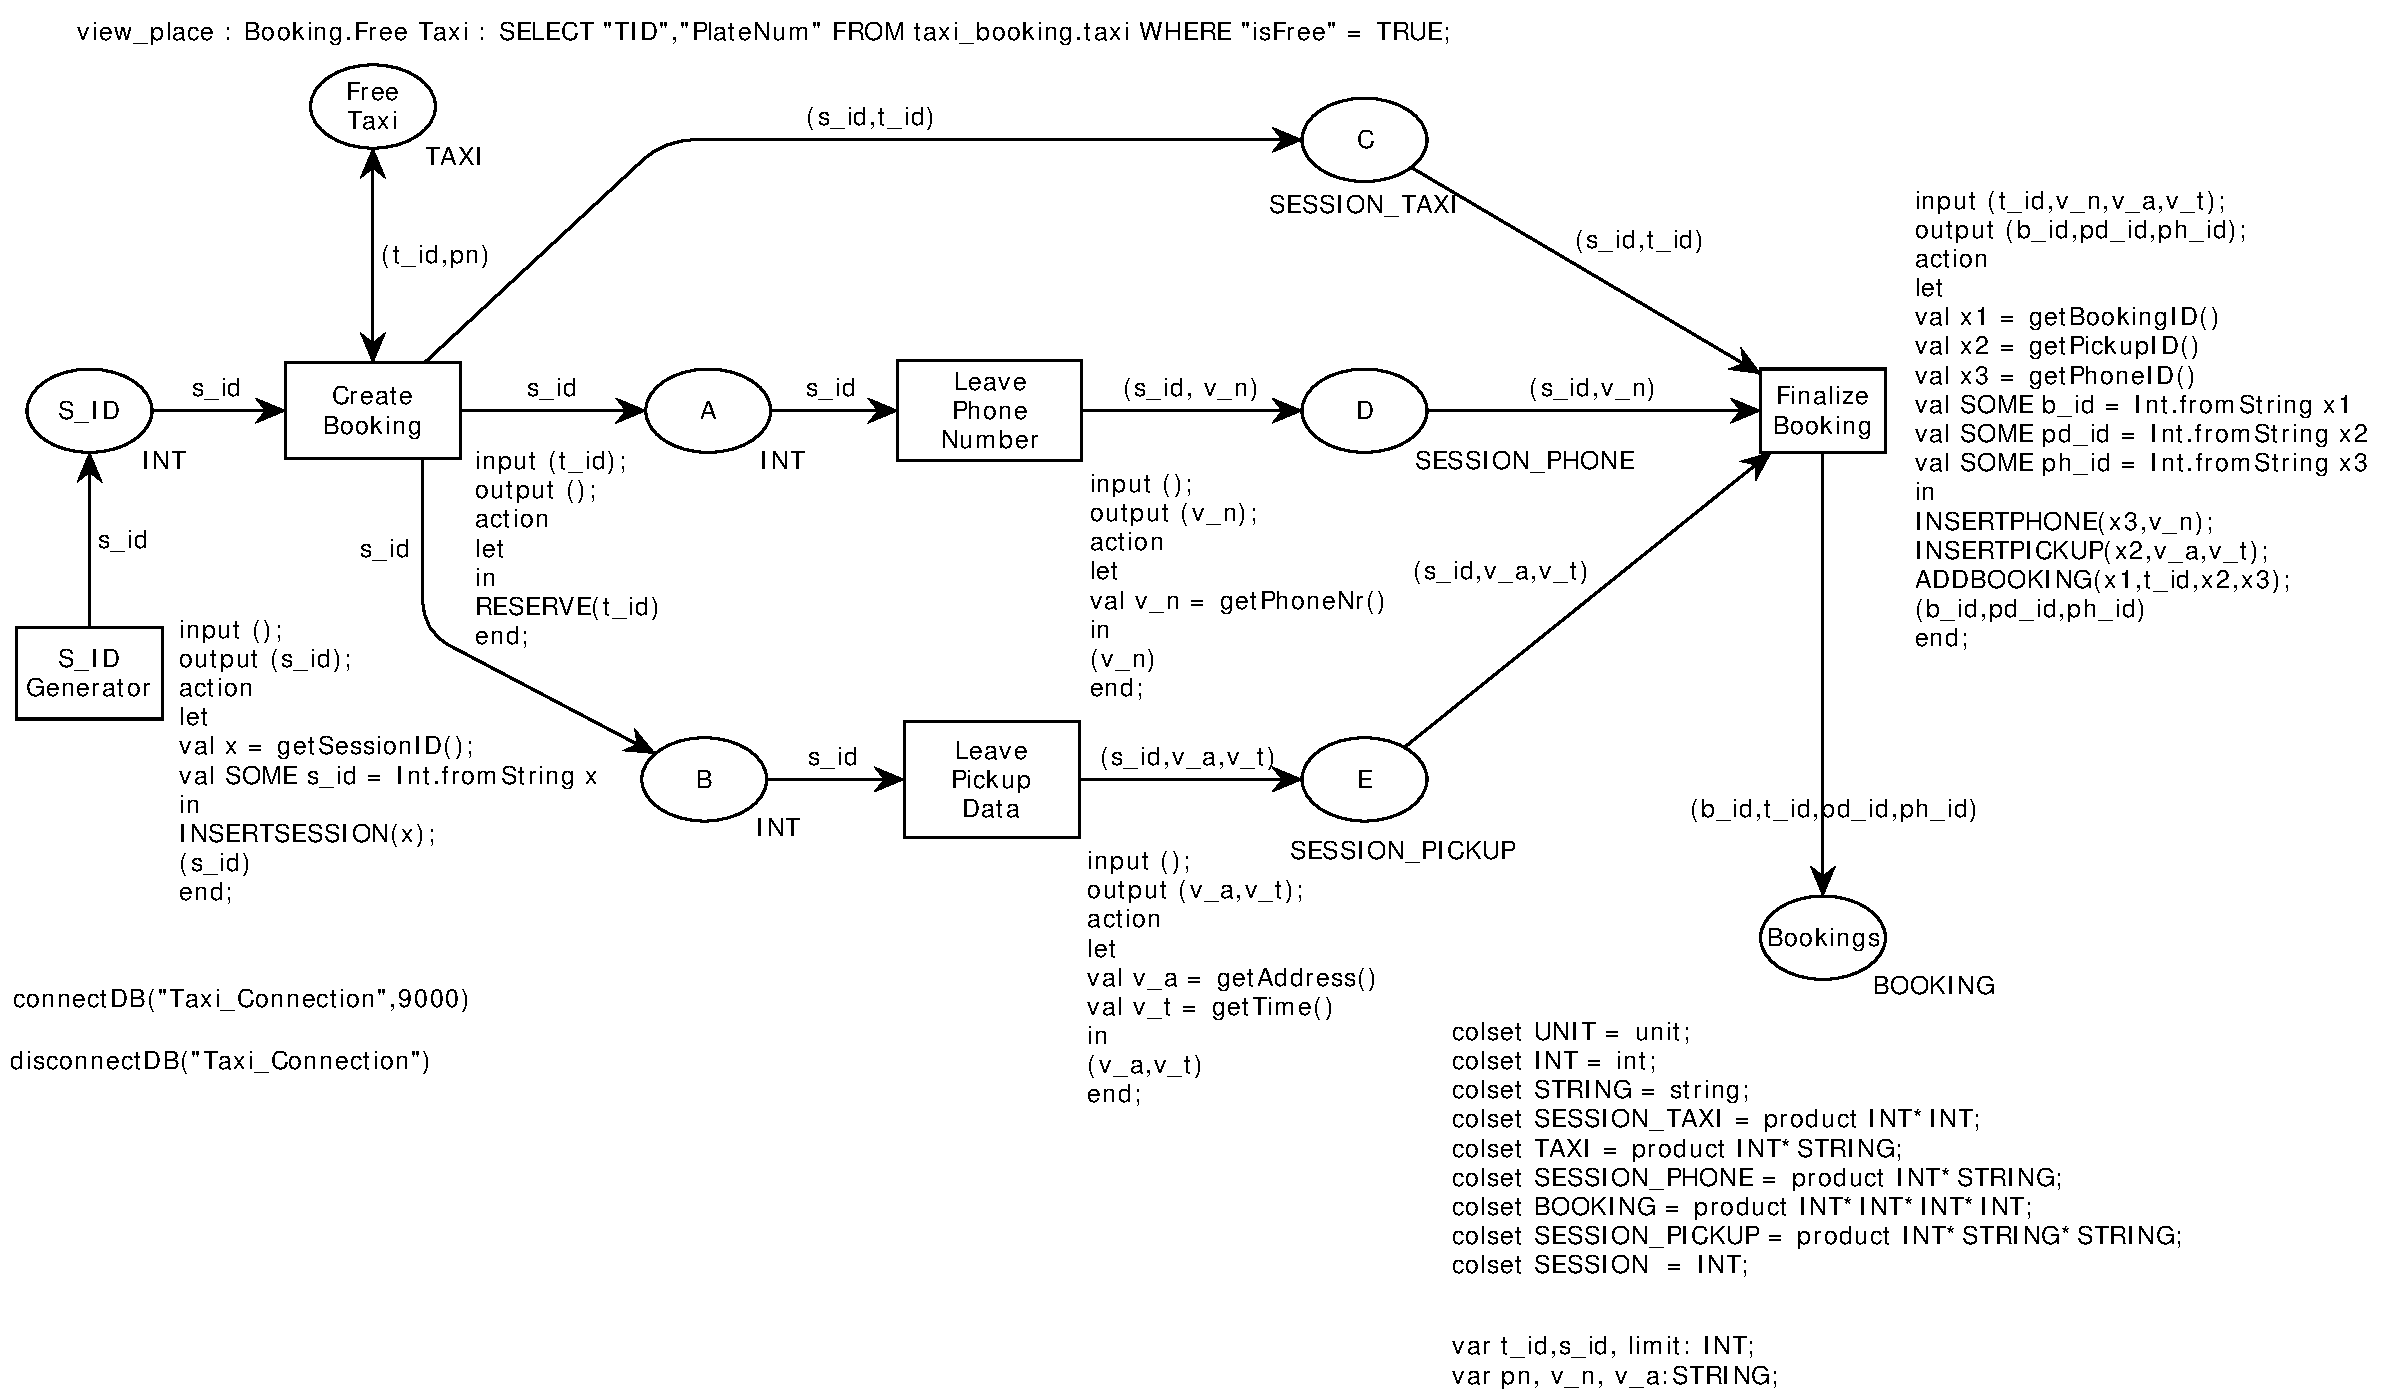
\includegraphics[scale = 0.35]{DBN_Impl_executable_model.pdf}
	\caption{Executable DB-net model for taxi booking}
	\label{fig:DBN_Impl_executable_model}
\end{figure}

\begin{figure}[!htbp]
	\centering
	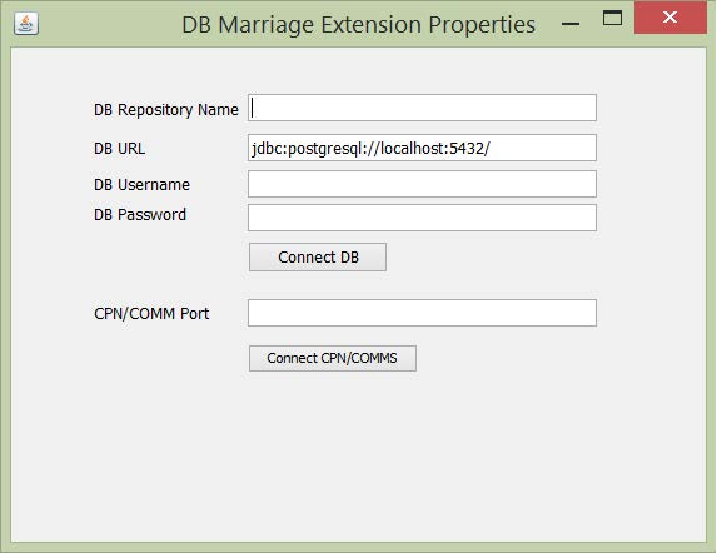
\includegraphics[scale = 0.75]{DBN_Impl_Extension_Dialog.pdf}
	\caption{Interface to provide connection parameters}
	\label{fig:DBN_Impl_Extension_Dialog}
\end{figure}

\subparagraph*{\textnormal{In order to execute actions in the transitions, we need to set up another connection using Comms/CPN. As a rule, in the attempt to establish a connection, the first handshake needs to be made using the Comms/CPN APIs and then the JAVA process can connect to the specified port. So, first we execute the \textit{connectDB} code, written in the text box, using the ML tool, then we provide the port number to the interface (see Figure \ref{fig:DBN_Impl_Extension_Dialog}) and finally we connect. Once the connection is successful, the user can play the token game using simulation tool box provided in the CPN Tools. In the net, whenever, a transition is fired, the view place automatically gets updated.}}

\subparagraph*{\textnormal{In this chapter, we discussed the implementation of DB-nets using CPN Tools extension and JAVA process. Using the mentioned modelling techniques, one can perform the simulation of DB-nets model in CPN Tools. In the next chapter, we will cover the analysis of DB-nets.}}

%%\begin{comment}
%\subsection{Architecture}
%\label{subsec:DBN_Impl_Architecture}
%\paragraph*{\textnormal{In this section, we present an idea for the implementation of different layers of DB-nets. In Figure \ref{fig:DBN_Impl_Mapping_Framework}, the DB-netlayers are mapped to their corresponding implementation paradigm. The persistence layer is modelled in PostgresSQL which is a relational database management system (RDBMS). The data logic layer is implemented as a JAVA application and for the control layer, we use CPN Tools.}}
%
%\begin{figure}[!htbp]
%	\centering
%	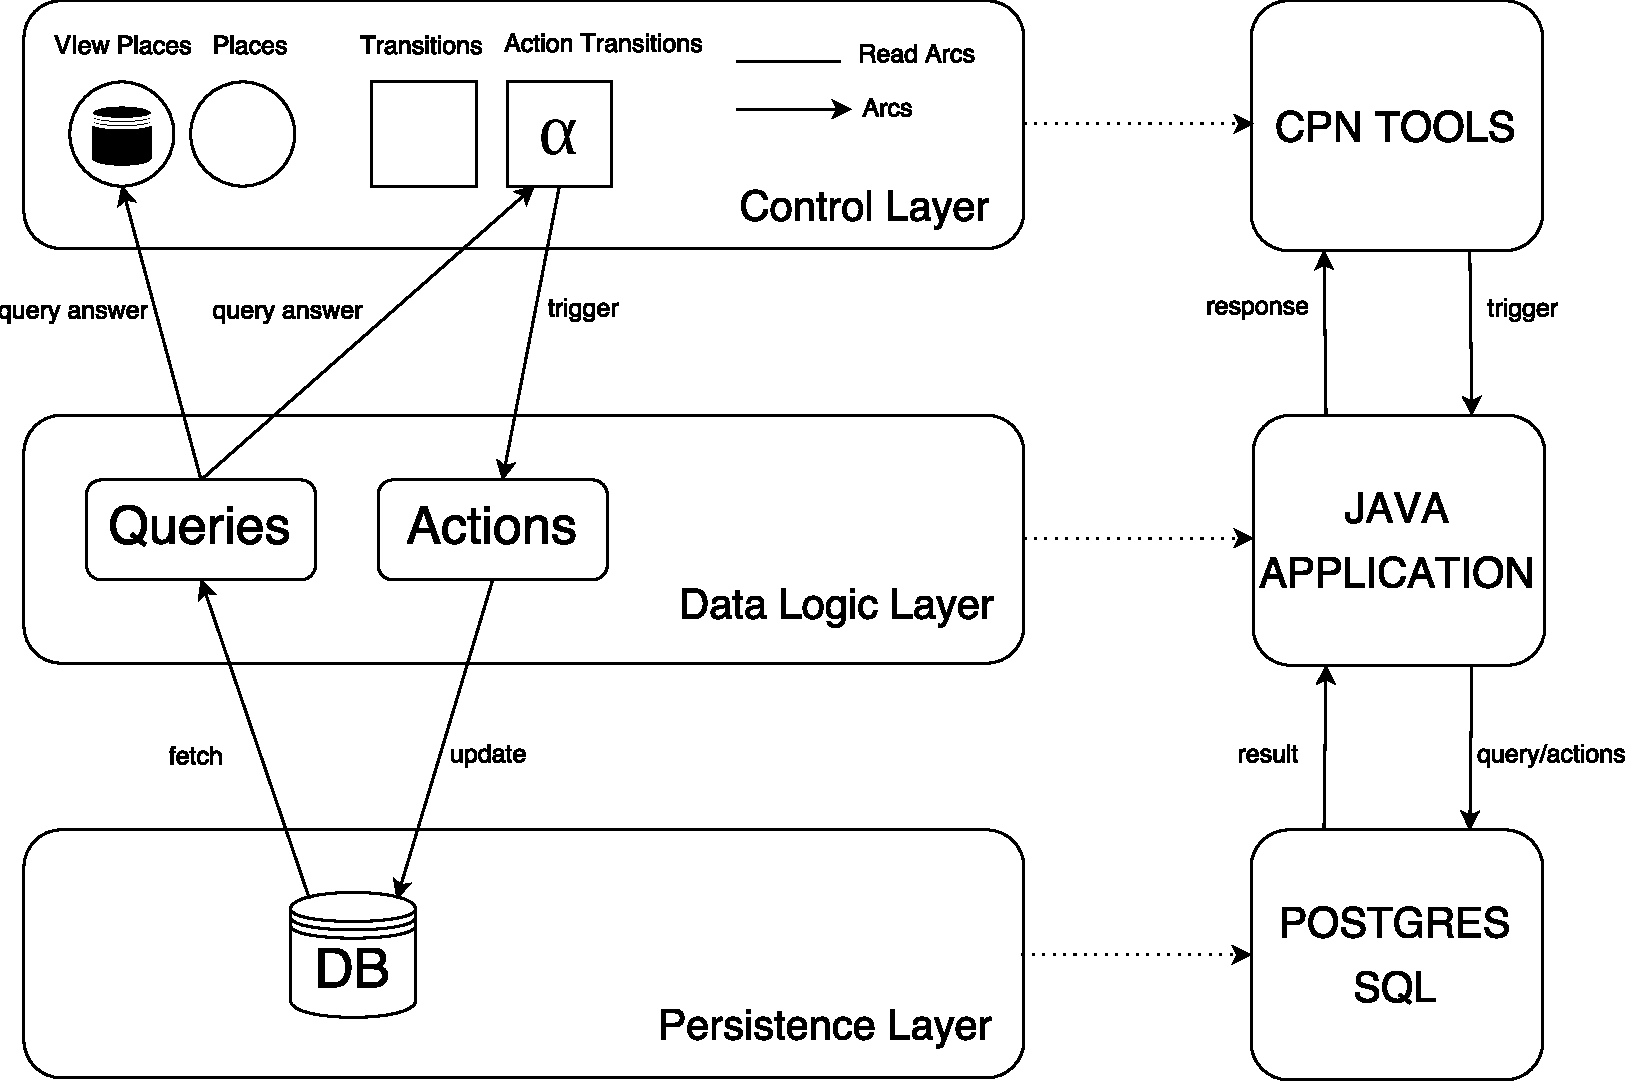
\includegraphics[scale = 0.35]{DBN_Impl_Mapping_Framework.pdf}
%	\caption{The mapping of db-net framework}
%	\label{fig:DBN_Impl_Mapping_Framework}
%\end{figure}
%
%\subparagraph*{\textnormal{The JAVA application comprises of the CPN Tools extension along with JAVA/CPN. JAVA/CPN allows JAVA processes to communicate with CPN Tools through Comms/CPN \footnote{Comms/CPN is a Standard ML library that augments Design/CPN with the necessary infrastructure to establish communication between CPN models and external processes. For source code of Comms/CPN, refer \cite{CPN_Tools_Comms/CPN}.} (refer \cite{gallasch2001comms}). The communication architecture between CPN Tools and JAVA/CPN is shown in Figure \ref{fig:DBN_Impl_CPNTools_Comms_JAVACPN_Comm}. CPN Tools use CPN-ML (a modified version of SML) as their programming language and Comms/CPN library is written in SML(compatible with CPN-ML). Comms/CPN use TCP/IP protocol to send/receive messages over a specified port. JAVA/CPN is a library, written in JAVA, is used to listen to send/receive messages through the specified port.}}
%
%\begin{figure}[!htbp]
%	\centering
%	
\includegraphics[scale = 0.35]{DBN_Impl_CPNTools_Comms_JAVACPN_Comm.pdf}
%	\caption{Communication between CPN Tools, Comms/CPN and JAVA/CPN}
%	\label{fig:DBN_Impl_CPNTools_Comms_JAVACPN_Comm}
%\end{figure}
%
%\subparagraph*{\textnormal{Figure \ref{fig:DBN_Impl_Java_App_Division} shows the framework through which the communication among different components takes place. Comms/CPN is used to connect to external environment/processes, which could possibly be web services etc, for data acquisition.\todo{AR:why for simplicity? AS:removed} Instead connecting to web services, we connect JAVA/CPN to database.\todo{AR: What did you want to say by that sentence? In our case Comms/CPN is just used to connect to DBs.\\AS:modified} We also modify JAVA/CPN and write our JAVA functions in order to facilitate data acquisition.\todo{how do you modify Comms/CPN? do you really expose your APIs like a web-service? it's just that I've never seen "expose" used in any other context but web services.\\AS:removed the exposed word} For example, while booking a taxi, when we fire \textit{Finalize Booking} transition, we add the booking with an id which is unique to the \textit{BOOKING} table, thus consulting the table for the ids which are not taken. Whereas, in order to receive the phone number of the customer, we don't need to consult the database and we use our function \textit{randomInt}.\todo{AR: randomInt is a function, right? also, try to come up with some special style for functions etc.\\AS: special style for functions?} In order to execute actions, one has to use the functions provided alongside JAVA/CPN. The query attached to a view place is processed by CPN Tools extension and the marking is returned as an answer to the corresponding query. For our use, we adopt the framework presented in Figure \ref{fig:DBN_Impl_Layer_Framework}.}}
%\begin{figure}[!htbp]
%	\centering
%	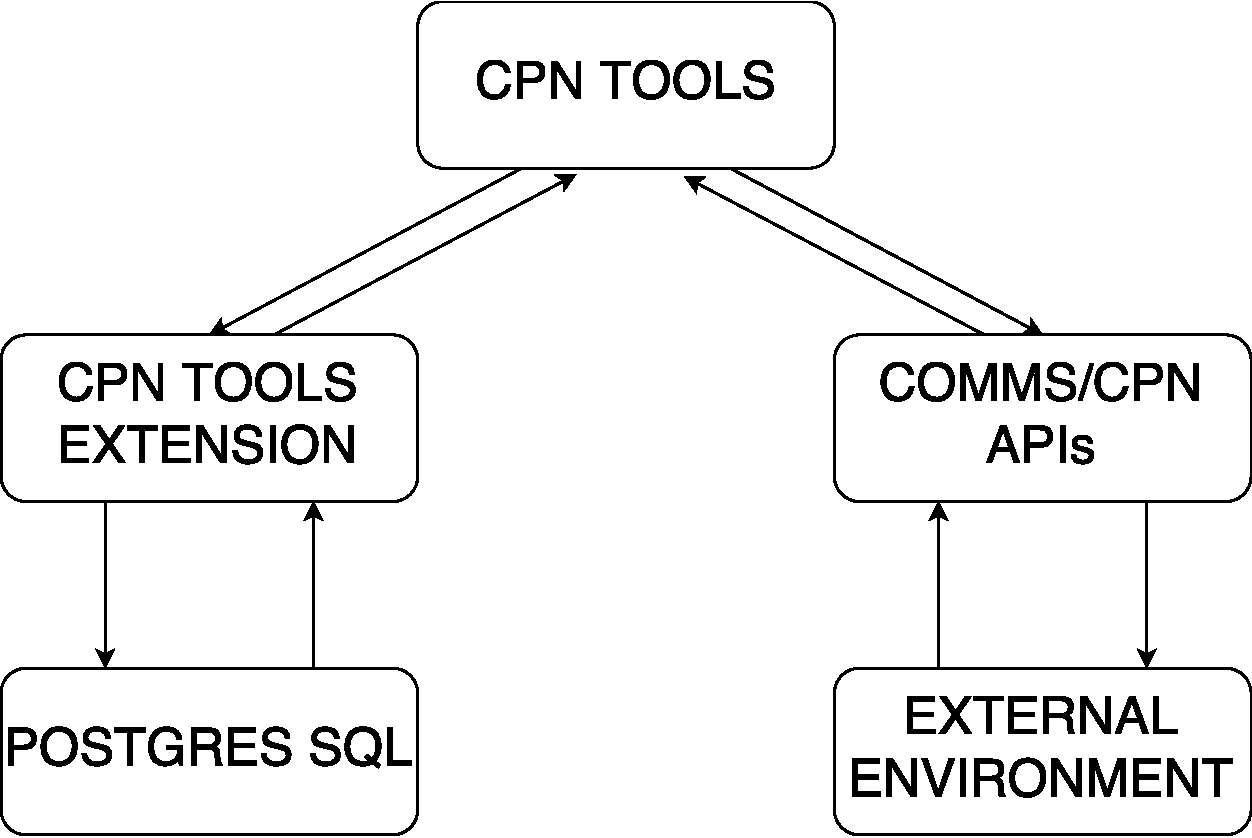
\includegraphics[scale = 0.35]{DBN_Impl_Java_App_Division.pdf}
%	\caption{Interconnectivity between different different components}
%	\label{fig:DBN_Impl_Java_App_Division}
%\end{figure}
%\begin{figure}[!htbp]
%	\centering
%	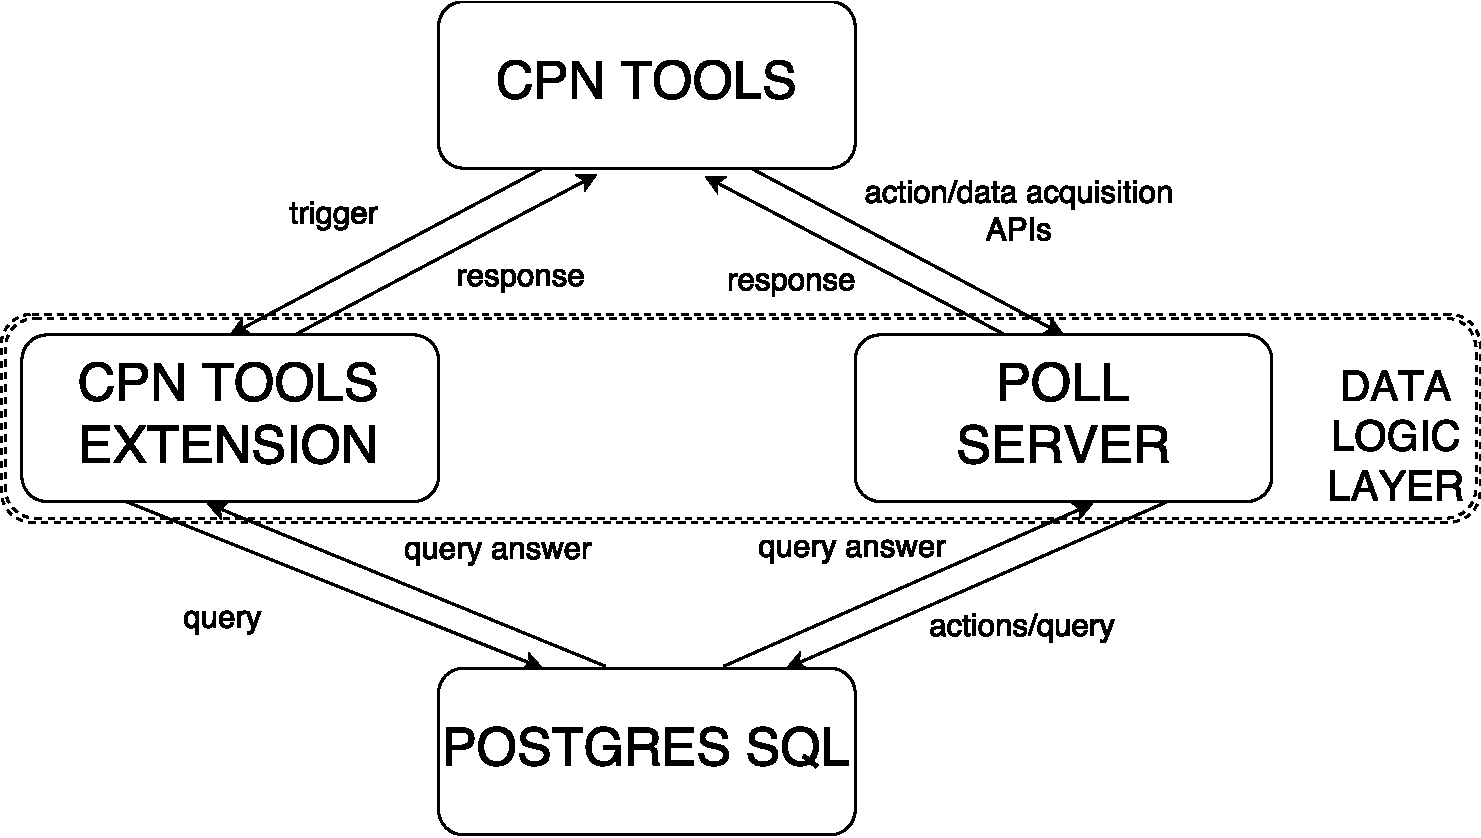
\includegraphics[scale = 0.35]{DBN_Impl_Layer_Framework.pdf}
%	\caption{Data logic layer division}
%	\label{fig:DBN_Impl_Layer_Framework}
%\end{figure}
%
%\section{Implementation}
%\label{sec:DBN_Impl_Impl}
%\subsection*{Persistence Layer}
%\label{subsec:DBN_Impl_persistence_layer}
%\paragraph*{\textnormal{The persistence layer is modelled in Postgres (an open source object-relational database management system, refer \cite{Postgres}). We name our database schema as \bdsq{taxi\_booking} (see Figure \ref{fig:DBN_Impl_Persistence_Layer}) which contains tables and constraints. The table \textit{session} contains the generated session ids for each booking session. The table \textit{taxi},\textit{phone} and \textit{pickup\_data} contains the information regarding taxi, customer's phone details and pickup details. Table \textit{booking} contains data related to the final booking. As indicated(see Figure \ref{fig:DBN_Impl_Persistence_Layer}), the relational schema also contains primary key and foreign key constraints. \todo{AR: fix the sentence\\AS: fixed}\todo{AR: first of all, you don't need to explain what SQL means. then, it's not enough to say that updates are performed using SQL. it's quit an obvious statement given that you are working with a relational DB. a certain update occurs after a corresponding action has been successfully executed. and then you discuss it in details later on.\\AS:fixed}}}
%
%\begin{figure}[!htbp]
%	\centering
%	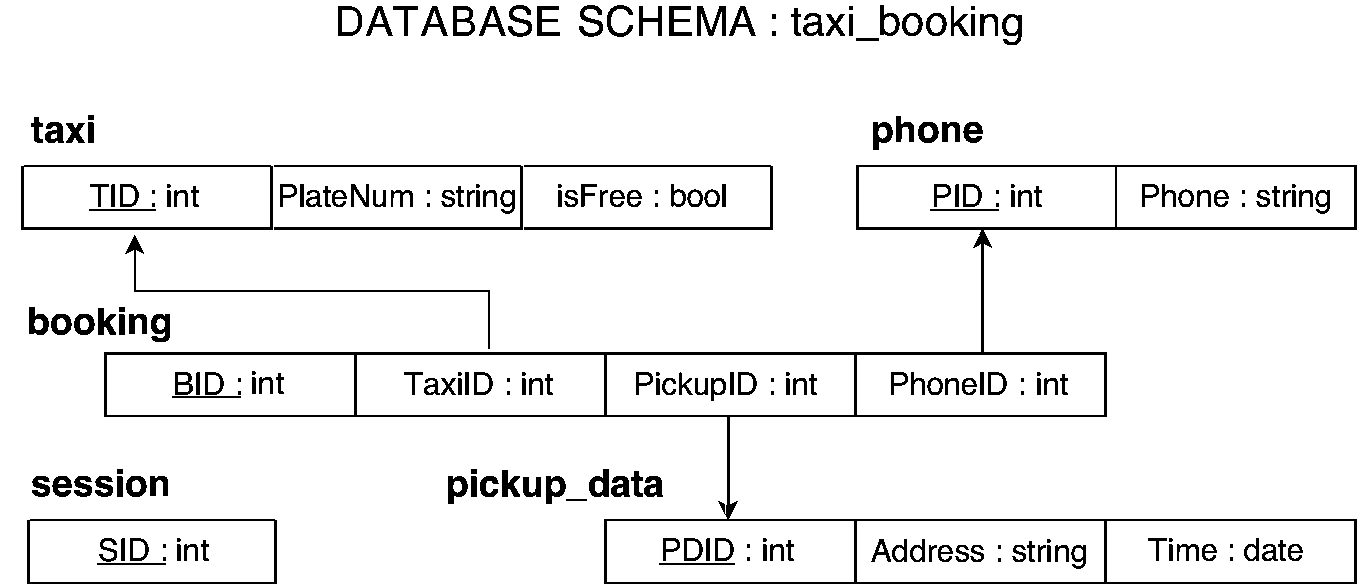
\includegraphics[scale = 0.45]{DBN_Impl_Persistence_Layer.pdf}
%	\caption{Database Schema for taxi booking example}
%	\label{fig:DBN_Impl_Persistence_Layer}
%\end{figure}
%
%\subsection*{Data Logic Layer and Control Layer}
%\label{subsec:DBN_Impl_control_layer}
%\paragraph*{\textnormal{Data logic layer is implemented as JAVA application and the control layer is implemented in CPN Tools. As shown in Figure \ref{fig:DBN_Impl_Java_App_Division} the data logic layer consists of two parts :
%		\begin{itemize}
%			\item CPN Tools extension
%			\item Comms/CPN APIs
%		\end{itemize}
%}}
%\subsubsection*{CPN Tools extension}
%\subparagraph*{\textnormal{In CPN Tools, the three major components are:
%		\begin{itemize}
%			\item GUI
%			\item Simulator
%			\item Extension
%\end{itemize}}}
%\subparagraph*{\textnormal{The modelling and execution of any CP nets depends on the interaction between GUI and Simulator. On the other hand, extensions are used to provide user-specific functionality in terms of simulation(execution) or modelling(GUI). \todo{all these pattern numbers are confusing. either one should present all the patterns in the appendix, or not even mention concrete references. AS: stuck to one} We design our extension on the communication pattern\footnote{Other communication patterns are mentioned in \cite{CPN_Tools_Extension}} presented in Figure \ref{fig:DBN_Impl_Extension_Communication_Pattern}.}}
%\begin{figure}[!htbp]
%	\centering
%	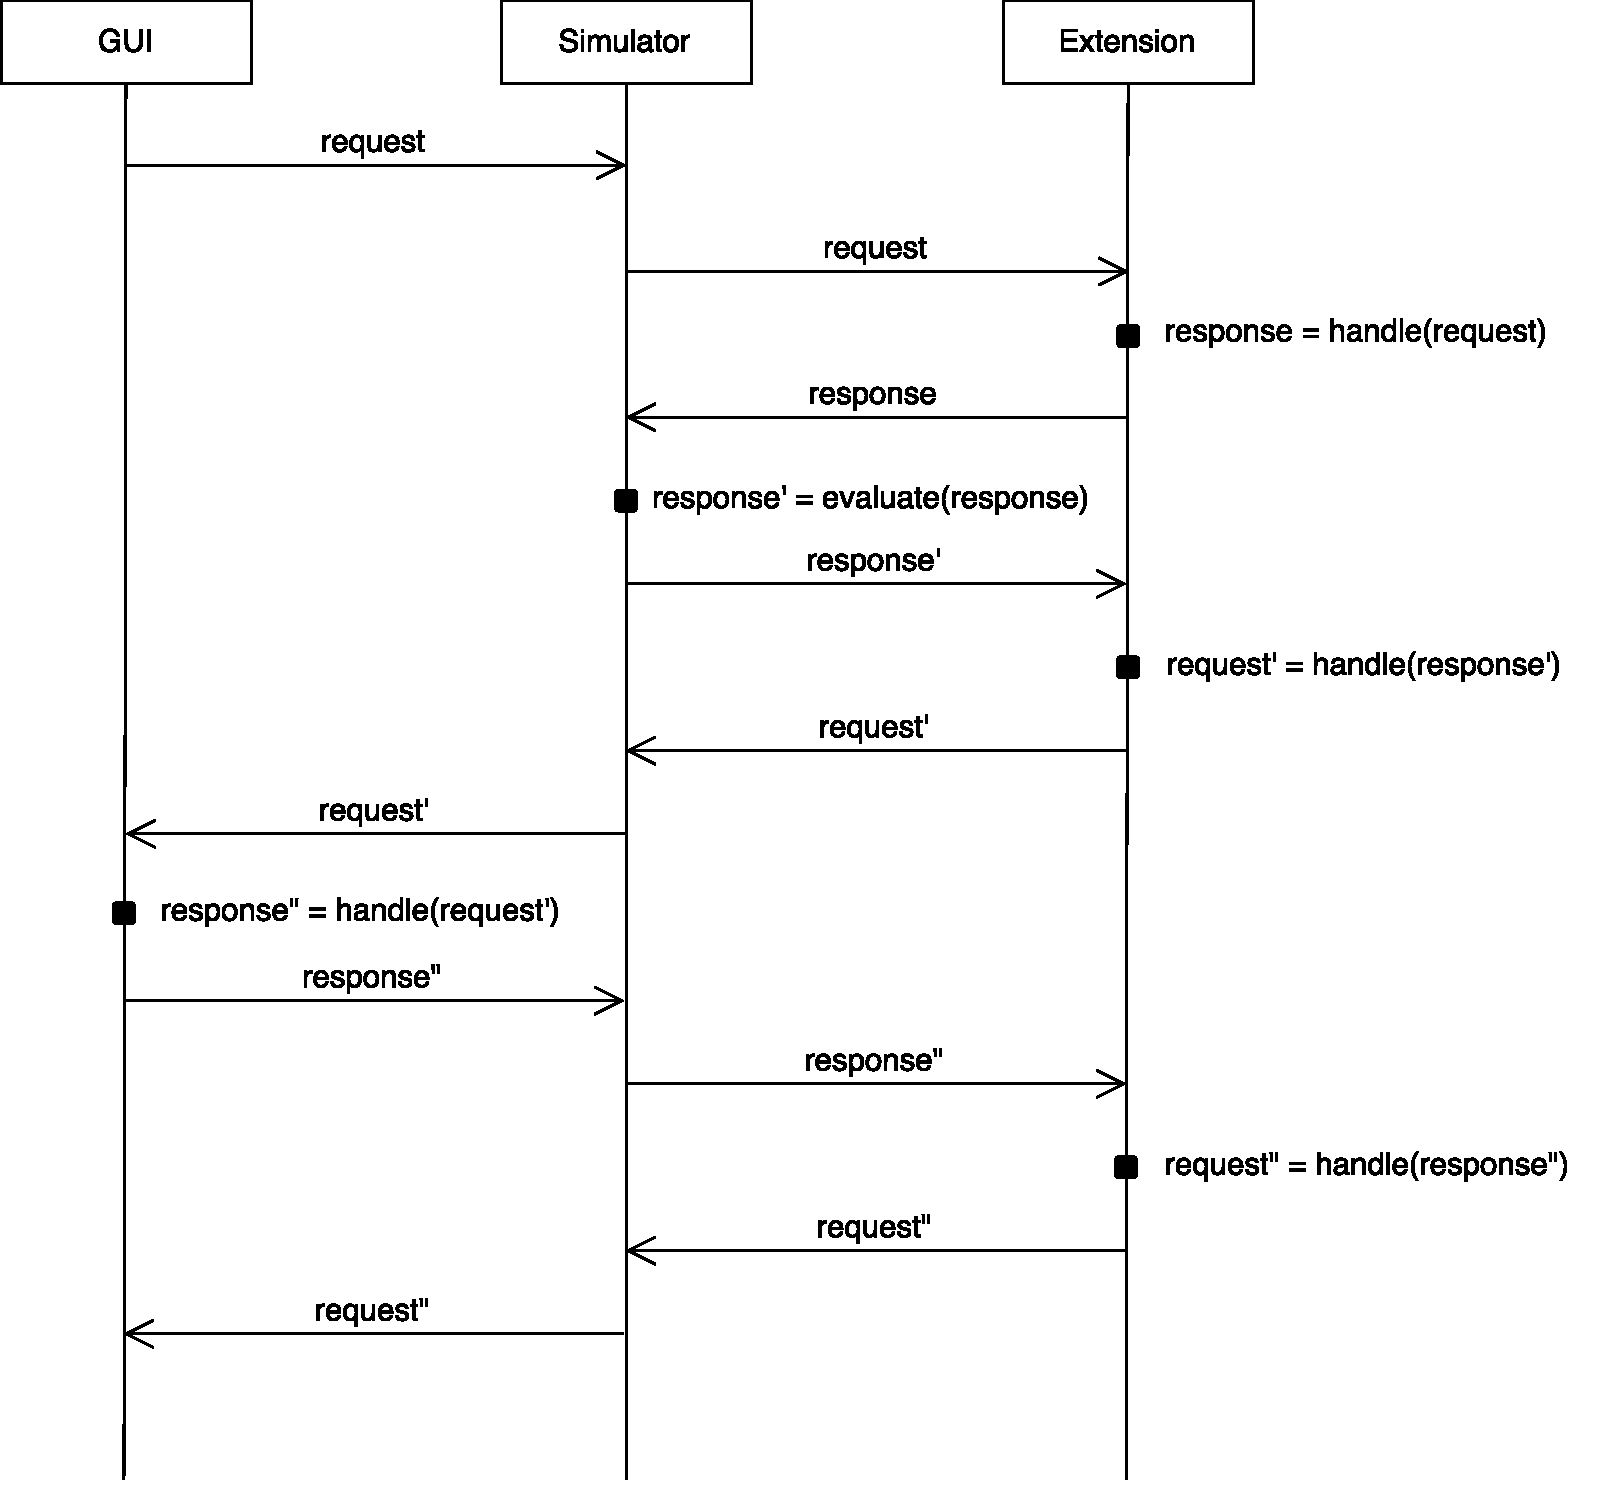
\includegraphics[scale = 0.40]{DBN_Impl_Extension_Communication_Pattern.pdf}
%	\caption{Communication Pattern of CPN Tools extensions}
%	\label{fig:DBN_Impl_Extension_Communication_Pattern}
%\end{figure}
%
%\subparagraph*{\textnormal{The responsibility of the extension is to look for changes in the DB-net model. \todo{fix this sentence}For example, changes related to modelling such as defining view places, declaring variables and colour sets, to execution events such as firing of transitions, the enabledness of transition etc., the extension listens to such events. Such \textit{requests}\footnote{We call events which is of our interests as \textit{requests}.}(modelling and execution)\todo{you should probably better define requests mentioned in Fig. 4.6} are passed from GUI to the extension via simulator. The extension takes appropriate response and passes on to the simulator. Simulator checks whether the response could be safely incorporated by the GUI i.e. the request should not bring CPN Tools to an inconsistent state,\todo{what does it mean "compatible with the GUI"?} and returns its evaluation to the extension. Once the evaluation is received, the extension handles the evaluated response and makes a request to the GUI to update. Once the request is incorporated/rejected by GUI, the response is sent to the extension. Extension handles the received response and gives the control back to the GUI. We will look at an example for this communication pattern later in the chapter.}} 
%
%\subparagraph*{\textnormal{The extension is also responsible for maintaining the connection with the database and performing queries over them. The whole working of the extension depends on the listening to the packets forwarded by the simulator. To know more about low level implementation of this extension, refer {\color{red} give reference to the documentation}.}}
%
%\subsubsection*{Modelling View Places}
%\subparagraph*{\textnormal{View places are drawn like normal places in CPN Tools. Also, view places carry SQL query along themselves. The syntax to define a view place is:}}
%\subparagraph*{}
%\begin{lstlisting}[showstringspaces=false, language = ML, caption = Syntax : view place, captionpos=b]
%view_place : <PageName.PlaceName> : <Query>
%\end{lstlisting}
%
%\subparagraph*{\textnormal{The above declaration should be written with \bdsq{Text} tool. For example, in Figure \ref{fig:DBN_Impl_Control_Layer}, the declaration for the view place is written as:
%}}
%\subparagraph*{}
%\begin{lstlisting}[showstringspaces=false, language = ML, caption = Syntax : view place, captionpos=b]
%view_place : Booking.Free_Taxi : SELECT "TID","PlateNum" FROM taxi_booking.taxi WHERE "isFree" = TRUE;
%\end{lstlisting}
%
%\begin{comment}
%For view places, the attached queries is written with the help of \bdsq{Text} Tool \todo{In appendix,Also define the regex for defining the view places} (provided by CPN Tools)\todo{I think that mentioning one of the tools here is a bit redundant}. The queries attached to action transitions or view places are written in SQL. One such part showing view places and action transitions in the taxi boking model is presented in Figure \ref{fig:DBN_Impl_Control_Layer}.\todo[inline]{Figure 4.5 demonstrates...} With the help of Text Tool (provided in the auxiliary palette)\todo{why so many details about tools from CPNTools? I think that if someone wants to use CPNTools, she will definitely find Text Tool.}, we make a statement declaring the view place along with the name of the place\todo{here you should explain better (without any footnotes) how one can define a view place} \footnote{The name of the view place is declared by adding the page name as the prefix (see Figure \ref{fig:DBN_Impl_Control_Layer}).}. In the figure\todo{which figure?}, the view place \textit{Free\_Taxi} is connected to the action transition \textit{Create Booking}. The query attached to the view place is:
%\end{comment}
%
%\begin{figure}[!htbp]
%	\centering
%	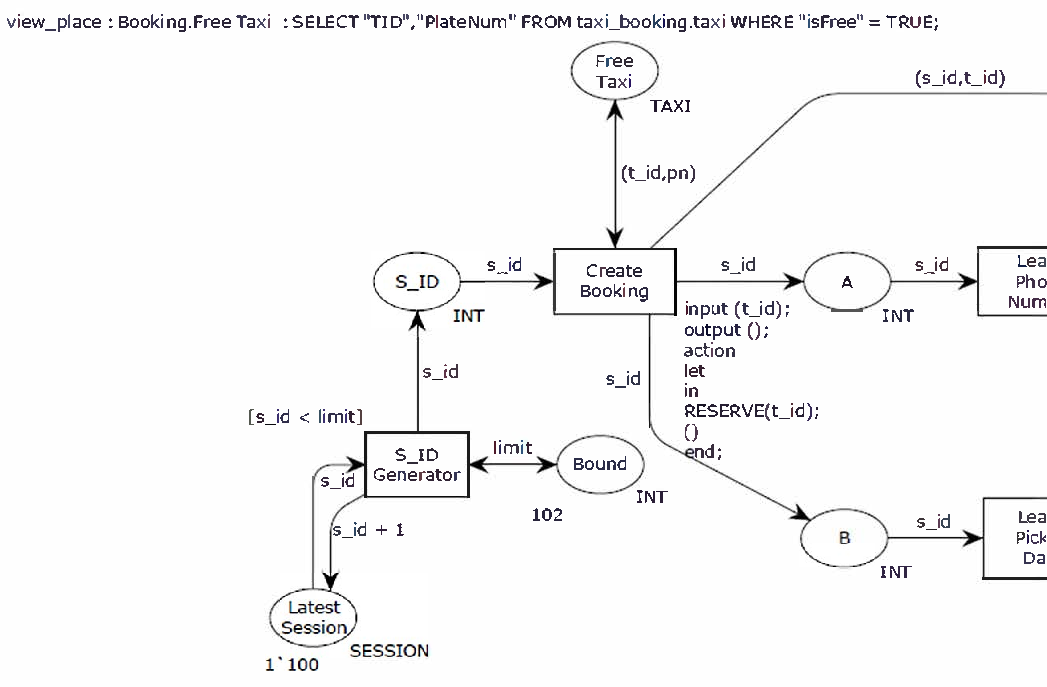
\includegraphics[scale = 0.60]{DBN_Impl_Control_Layer.pdf}
%	\caption{View Place, Action Transition and Read Arcs representation}
%	\label{fig:DBN_Impl_Control_Layer}
%\end{figure}
%
%\subparagraph*{\textnormal{Let's see the example of populating the view places using the communication pattern presented in Figure \ref{fig:DBN_Impl_Extension_Communication_Pattern}. When we declare a view place (see Figure \ref{fig:DBN_Impl_Control_Layer})\todo{are view places declared dynamically?}, the extension listens to the GUI and determines the declaration. In this case, the \textit{request} is passed from the GUI to the extension via simulator. The extension \textit{handles} the request and takes appropriate \textit{response} by fetching the marking(for the view place) from the database. However, at this stage, extension doesn't know if the markings are compatible with the colour set of the view place. In order to verify, if the marking is compatible to the colour set of the view place, the \textit{response} is passed to the simulator. The simulator evaluates (verification of the marking) the \textit{response} and provides its decision (\textit{response\textquotesingle}) to the extension whether the marking is compatible to the colour set of the view place. On receiving the evaluation, extension handles it and in case the marking is compatible, it creates a new request(\textit{request\textquotesingle}) to change the marking of the view place and passes on to the GUI via simulator. On receiving the new request, the GUI changes the marking of the view place. After incorporating the request (by changing the marking of view place), the GUI sends a response(\textit{response\textquotedbl}) to the extension whether the request (\textit{request\textquotesingle}) was successful or unsuccessful. Upon receiving the response, the extension handles it and gives back the control to the GUI.}}
%
%\subsubsection*{Modelling Action Transitions}
%\subparagraph*{\textnormal{The actions which are attached to the action transitions are modelled using ML functions. The code segment of transitions helps us in defining actions. The code segment has \textit{input}, \textit{output} and \textit{action} part. The input variables(the variables of interest) should be mentioned in the \textit{input} part and the fresh variables should mentioned in the \textit{output} part. The \textit{action} part has \textit{let\ldots in \ldots end} construct\footnote{This construct is similar to the construct for ML functions.}. The data for the fresh variables is acquired in the \textit{let} part whereas \textit{in} part contains \textit{actions}. Just before the \textit{end} part, the fresh variables(if any) should be written within parentheses in order corresponding to the variables in the \textit{output} part. In Figure \ref{fig:DBN_Impl_Control_Layer}, the \textit{let\ldots in \ldots end} part of the \textit{Create Booking} transition is written as:}}
%
%\subparagraph*{}
%
%\begin{lstlisting}[showstringspaces=false, language = ML, caption = Code Segment : \textit{Create Booking} transition, captionpos=b, label = lst:DBN_Impl_Create_Booking_code_segment, numbers=left,
%stepnumber=1]
%input (t_id);
%output ();
%action
%let
%in
%RESERVE(t_id);
%()
%end;
%\end{lstlisting}
%
%\subparagraph*{\textnormal{The \textit{Create Booking} transition has \textit{RESERVE} action, which takes the selected taxi id as parameter and reserves it. The \textit{RESERVE} action is defined as an ML function:
%}}
%
%\subparagraph*{}
%
%\begin{lstlisting}[showstringspaces=false, language = ML, caption = RESERVE action, captionpos=b, label = lst:DBN_Impl_RESERVE_action_query]
%fun RESERVE(t_id) = exQuery("UPDATE taxi_booking.taxi SET \"isFree\" = FALSE WHERE \"TID\" ="^ Int.toString t_id^";");
%\end{lstlisting}
%
%\subparagraph*{\textnormal{\textit{exQuery} is an ML function which takes the query\footnote{In the query, (see Listing \ref{lst:DBN_Impl_RESERVE_action_query}), the {\textbackslash \textquotedbl} symbol is used in ML to represent double quotes in string where as $\string^$ symbol is used to concatenate two strings.} as a parameter and passes it to Comms/CPN for execution.\todo{AR:passes what? \\ AS:reframed} For example, for $t\_id = 47552$, the query to be passed would be :}}
%
%\subparagraph*{}
%\begin{lstlisting}[showstringspaces=false, language = SQL, caption = RESERVE action query simplification, captionpos=b, label = lst:DBN_Impl_RESERVE_action_query_ex]
%UPDATE taxi_booking.taxi SET "isFree" = FALSE WHERE "TID" = 47552;
%\end{lstlisting}
%
%\subparagraph*{\textnormal{The \textit{exQuery} function internally calls the Comms/CPN APIs, thus passing actions through Comms/CPN to the database. In order to execute actions attached to action transitions and acquiring data from the external environment we use Comms/CPN. Comms/CPN provide a set of APIs which are:
%		\begin{enumerate}
%			\item \textit{openConnection} - allows users to connect to external process as a client. It takes three parameters, the first is the connection name which is a unique identifier, the second is the host name and the third is the port number.  
%			\item \textit{acceptConnection} - allows external processes to connect to CPN Tools GUI. It takes two parameters, first is the connection name which is a unique identifier and the second one is the port number where the connection needs to be established.
%			\item \textit{send} - allows users to send any type of data to external processes. It takes three parameters, the first is the connection identifier followed by the data to be sent. The last parameter is the encoding function which is used to encode the data to a byte stream.
%			\item \textit{receive} - allows users to receive any type of data from external processes.It takes two parameters, the first is the connection identifier followed by a parameter specifying the decoding function to  decode the received data(in byte stream) from the connection.
%			\item \textit{closeConnection} - allows users to close a connection. Takes a single parameter which specifies name of the connection to be closed.
%\end{enumerate}}}
%
%\subparagraph*{\textnormal{In our case, we don't use \textit{openConnection} since we don't work in a remote architecture. \todo{AR: you should explain what does it mean to be a client here.\\AS:Here I am really not sure, it is in the sense that CPNTools is running on one machine and the COMMS server is running on other machine, and if we want to connect them remotely. I never tried this architecture, involves some kind of networking.}The \textit{send} and \textit{receive} APIs send and receive data in \textit{string} data-type. \textit{closeConnection} closes the connection. In order to set up the connectivity with Comm/CPN and CPN Tools, we create ML function which calls Comms/CPN APIs. For example, we create connectDB\footnote{While calling \textit{acceptConnection} we assume that the connection name is \bdsq{Taxi\_Connection}. We will use this connection name through out our example.} and disconnectDB function in ML which can be defined as:}}
%\subparagraph*{}
%\begin{lstlisting}[showstringspaces=false, language = ML, caption = Accept/Close connection functions, captionpos=b, label = lst:DBN_Impl_acc_close_conn_func]
%fun connectDB(connName, port) = acceptConnection(connName, port);
%fun disconnectDB(connName) = closeConnection(connName);
%\end{lstlisting}
%
%\subparagraph*{\textnormal{We encapsulate the name of the functions for data acquisition (\textit{funcAPI}) in a string and send it using the Comms/CPN APIs\footnote{We modify Comms/CPN source code and add our functions}. On receiving the string, the decoder decodes the string and calls the corresponding data acquisition APIs. The set of ML functions\todo{you need to explain that comms works through ML. moreover, the function you define below are of two different kinds. getFromDB and exQuery are "canonical" functions that remain intact for every db-net model, while getRandom is specific for your concrete example.}\footnote{In order to make our functions consistent with the provided Comms/CPN APIs we use string as the data type while passing the parameters.} which internally calls the Comms/CPN APIs are:
%		\begin{enumerate}
%			\item \textit{getRandom} - takes two parameters: \textit{funcAPI} and \textit{length}. The \textit{funcAPI} can be either \textit{randomInt}, \textit{randomString} or \textit{randomTime}. Based on the \textit{funcAPI}, data logic layer decides which function should be called and returns the result.
%			\item \textit{getFromDB} - takes four parameters: \textit{tableName}, \textit{columnName}, \textit{funcAPI} and \textit{length}. Currently the supported funcAPI is \bdsq{getFromDB} to get a unique identifier of given length for the specified \textit{tableName} and \textit{columnName}.
%			\item \textit{exQuery} - takes two parameters: \textit{funcAPI} and \textit{query}. Currently the supported funcAPI is \bdsq{exQuery} to execute the given query.
%\end{enumerate}}}
%
%\subparagraph*{\textnormal{The use of \textit{getRandom} and \textit{getFromDB} is optional and it depends on the requirement of the modeller but in order to execute queries, one should use \textit{exQuery}. The ML function for \textit{exQuery}, which can be used in the \textit{RESERVE} action mentioned in the Listing \ref{lst:DBN_Impl_RESERVE_action_query}, is:}}
%
%\subparagraph*{}
%\begin{lstlisting}[showstringspaces=false, language = ML, caption = exQuery function, captionpos=b, label = lst:DBN_Impl_exquery_func]
%fun exQuery(funcAPI, query) = ConnManagementLayer.send("Taxi_Connection", funcAPI^"?"^query, stringEncode);
%\end{lstlisting}
%
%\subparagraph*{\textnormal{The \bdsq{?}\todo{in general, a question mark is not the best solution due to ambiguities that my rise while using different SQL dialects. AS: which symbol should I use? Can you give me examples of ambiguities? I have heard about "?" being used in SPARQL} sign in the function is used to provide a marker to the data acquisition functions which helps in parsing the string received from the Comms/CPN.\footnote{The first parameter should be funcAPI, followed by other parameters separated by \bdsq{?}.} Using the example given in Listing \ref{lst:DBN_Impl_RESERVE_action_query_ex}, calling \textit{exQuery} can be seen as :}}
%
%\subparagraph*{}
%\begin{lstlisting}[showstringspaces=false, language = SQL, caption = exQuery Example, captionpos=b, label = lst:DBN_Impl_exquery_func_ex]
%ConnManagementLayer.send(Taxi_Connection, exQuery?UPDATE taxi_booking.taxi SET "isFree" = FALSE WHERE "TID" = 47552;, stringEncode);
%\end{lstlisting}
%
%\subparagraph*{\textnormal{Other functions such as \textit{getFromDB} and \textit{getRandom} can be written in ML as:}}
%
%\subparagraph*{}
%
%\begin{lstlisting}[showstringspaces=false, language = ML, caption = Data Acquisition Functions, captionpos=b, label = lst:DBN_Impl_data_acq_functions]
%fun getFromDB(funcAPI, t_name, c_name, length) =
%(ConnManagementLayer.send("Taxi_Connection", "getFromDB"^"?"^t_name^"?"^c_name^"?"^funcAPI^"?"^length, stringEncode);
%ConnManagementLayer.receive("Taxi_Connection", stringDecode));
%fun getRandom(funcAPI, length) = (ConnManagementLayer.send("Taxi_Connection", "getRandom"^"?"^funcAPI^"?"^length, stringEncode);
%ConnManagementLayer.receive("Taxi_Connection", stringDecode));
%\end{lstlisting}
%
%\begin{comment}
%content...
%
%\subsection{Data Logic Layer}
%\paragraph*{\textnormal{As shown in Figure \ref{fig:DBN_Impl_Java_App_Division} the data logic layer consists of two parts :
%\begin{itemize}
%\item CPN Tools extension
%\item Comms/CPN APIs
%\end{itemize}
%}}
%\subsubsection*{CPN Tools extension}
%\subparagraph*{\textnormal{In CPN Tools, the three major components are:
%\begin{itemize}
%\item GUI
%\item Simulator
%\item Extension
%\end{itemize}}}
%\subparagraph*{\textnormal{The modelling and execution of any CP nets depends on the interaction between GUI and Simulator. On other hand, extensions are used to provide user-specific functionality in terms of simulation(execution) or modelling(GUI). There are many communication patterns presented in \cite{CPN_Tools_Extension}, and we adopt a mixture of pattern 6,7 and 8 \todo{AR: all these pattern numbers are confusing. either one should present all the patterns in the appendix, or not even mention concrete references.\\AS:Removed} and design our extension on the pattern\footnote{Although, the pattern resembles to the pattern 9b, mentioned in \cite{CPN_Tools_Extension}, but it differs slightly from it.} presented in Figure \ref{fig:DBN_Impl_Extension_Communication_Pattern}.}}
%\begin{figure}[!htbp]
%\centering
%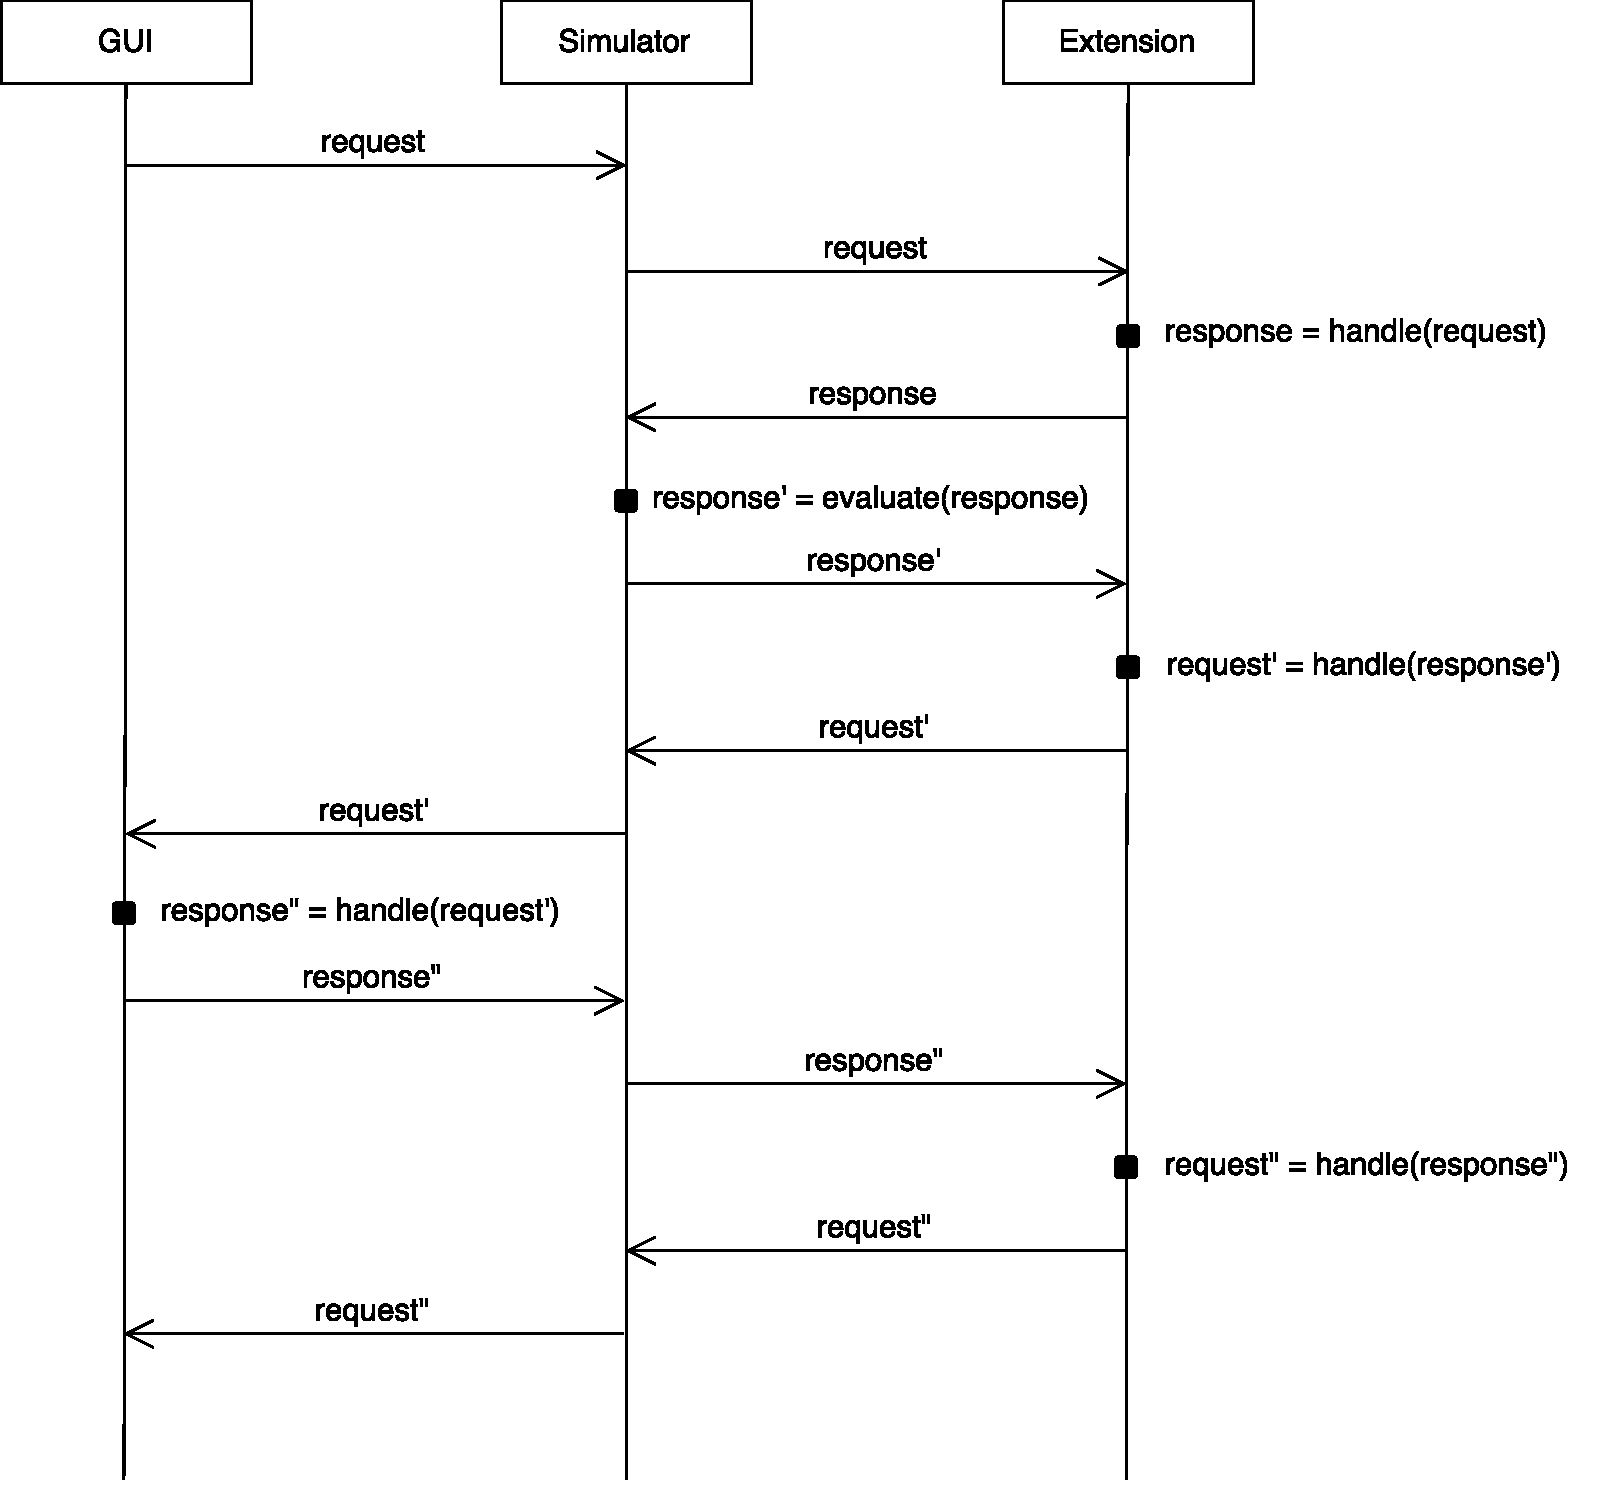
\includegraphics[scale = 0.40]{DBN_Impl_Extension_Communication_Pattern.pdf}
%\caption{Communication Pattern of CPN Tools extensions}
%\label{fig:DBN_Impl_Extension_Communication_Pattern_temp}
%\end{figure}
%
%\subparagraph*{\textnormal{The responsibility of the extension is to look for changes in the DB-net model. \todo{fix this sentence}For example, changes related to modelling such as defining view places, declaring variables and colour sets, to execution events such as firing of transitions, the enabledness of transition etc., the extension listens to such events. Such \textit{requests}\footnote{We call the events which is of our interests a \textit{requests}.}(modelling and execution)\todo{you should probably better define requests mentioned in Fig. 4.6} are passed from GUI to the extension via simulator. The extension takes appropriate response and passes on to the simulator. Simulator checks whether the response could be safely incorporated by the GUI i.e. the request should not bring CPN Tools to an inconsistent state,\todo{what does it mean "compatible with the GUI"?} and returns its evaluation to the extension. Once the evaluation is received, the extension handles the evaluated response and makes a request to the GUI to update. Once the request is incorporated/rejected by GUI, the response is sent to the extension. Extension handles the received response and gives the control back to the GUI.}}
%
%\subparagraph*{\textnormal{For instance, let's see the example of populating the view places using the communication pattern presented in Figure \ref{fig:DBN_Impl_Extension_Communication_Pattern}. When we declare a view place (see Figure \ref{fig:DBN_Impl_Control_Layer})\todo{are view places declared dynamically?}, the extension listens to the GUI and determines the declaration. In this case, the request is passed from the GUI to the extension via simulator. The simulator \textit{handles} the request and takes appropriate \textit{response} by fetching the marking(for the view place) from the database. This \textit{response} is passed to the simulator to check whether the marking is compatible to the view place (if the marking matches the colour set of the view place). The simulator evaluates the \textit{response} and provides its decision (\textit{response\textquotesingle}) to the extension. Extension creates a new request(\textit{request\textquotesingle}) to change the marking of the view place and passes on to the GUI. On receiving the new request, the GUI changes the marking of the view place. After incorporating the request (by changing the markings of view places), the GUI sends a response(\textit{response\textquotedbl}) to the extension whether the request (\textit{request\textquotesingle}) was successful or unsuccessful. Upon receiving the response, the extension handles it and gives back the control to the GUI.}}
%
%\subparagraph*{\textnormal{Apart from populating view places, extension is also responsible for maintaining the connection with the database and performing queries over them. The whole working of the extension depends on the listening to the packets forwarded by the simulator. To know more about low level implementation of this extension, refer {\color{red} give reference to the documentation}.}}
%
%\subsubsection{Comms/CPN APIs}
%\subparagraph*{\textnormal{In order to execute actions attached to action transitions and acquiring data from the external environment we use Comms/CPN. Comms/CPN provide a set of APIs which are:
%\begin{enumerate}
%\item \textit{openConnection} - allows users to connect to external process as a client. It takes three parameters, the first is the connection name which is a unique identifier, the second is the host name and the third is the port number.  
%\item \textit{acceptConnection} - allows external processes to connect to CPN Tools GUI. It takes two parameters, first is the connection name which is a unique identifier and the second one is the port number where the connection needs to be established.
%\item \textit{send} - allows users to send any type of data to external processes. It takes three parameters, the first is the connection identifier followed by the data to be sent. The last parameter is used to encode the data to a byte stream.
%\item \textit{receive} - allows users to receive any type of data from external processes.It takes two parameters, the first is the connection identifier followed by the parameter to  decode the received data(in byte stream) from the connection.
%\item \textit{closeConnection} - allows users to close a connection. Takes a single parameter which specifies name of the connection to be closed.
%\end{enumerate}}}
%\subparagraph*{\textnormal{In our case, we don't use \textit{openConnection} since we don't need to be a client. \todo{AR: you should explain what does it mean to be a client here.\\AS:Here I am really not sure, it is in the sense that CPNTools is running on one machine and the COMMS server is running on other machine, and if we want to connect them remotely. I never tried this architecture, involves some kind of networking.}. The send and receive APIs send and receive data in \textit{string} data-type. We encapsulate the name of required APIs for data acquisition (\textit{funcAPI}) in a string and send it using the Comms/CPN APIs\footnote{We modify Comms/CPN source code and add our APIs}. On receiving the string, the decoder decodes the string and calls the corresponding data acquisition APIs. The set of ML functions\todo{you need to explain that comms works through ML. moreover, the function you define below are of two different kinds. getFromDB and exQuery are "canonical" functions that remain intact for every db-net model, while getRandom is specific for your concrete example.}\footnote{In order to make our APIs consistent with the provided Comms/CPN APIs we use string while passing the parameters.} which internally calls the Comms/CPN APIs are:
%\begin{enumerate}
%\item \textit{getRandom} - takes two \textbf{string} parameters: \textit{funcAPI} and \textit{length}. The \textit{funcAPI} can be either \bdsq{randomInt} or \bdsq{randomString}. Based on the \textit{funcAPI}, data logic layer decides which function should be called and returns the result.
%\item \textit{getFromDB} - takes four parameters: \textit{tableName}, \textit{columnName}, \textit{funcAPI} and \textit{length}. Currently the supported funcAPI is \bdsq{getFromDB} to get a unique identifier of given length for the specified \textit{tableName} and \textit{columnName}.
%\item \textit{exQuery} - takes two parameters: \textit{funcAPI} and \textit{query}. Currently the supported funcAPI is \bdsq{exQuery} to execute the given query.
%\end{enumerate}}}
%
%\subparagraph*{\textnormal{
%\todo{you have to explain briefly before how to make comms work in a CPN model using ML} In order to create a connection with external applications using Comms/CPN, we create ML function with connection parameters. Similarly, we create an ML function for closing the connection. These two functions can be written as:}}
%
%\subparagraph*{}
%\begin{lstlisting}[showstringspaces=false, language = ML, caption = Accept/Close connection functions, captionpos=b, label = lst:DBN_Impl_acc_close_conn_func]
%fun connectDB(connName,port) = acceptConnection(connName,port);
%fun disconnectDB(connName) = closeConnection(connName);
%\end{lstlisting}
%
%\subparagraph*{\textnormal{While calling \textbf{acceptConnection} we assume that the connection name is \bdsq{Taxi\_Connection}\footnote{We will use this connection name through out our example.}.We create ML functions in CPN Tools, which encapsulates the required APIs(of the data logic layer) in a string and uses Comms/CPN APIs for sending or receiving. For example, the RESERVE action mentioned in the Listing \ref{lst:DBN_Impl_RESERVE_action_query}, the function \textit{exQuery} is written in ML (in CPN tools) as:
%}}
%
%\subparagraph*{}
%\begin{lstlisting}[showstringspaces=false, language = ML, caption = exQuery functions, captionpos=b, label = lst:DBN_Impl_exquery_func]
%fun exQuery(funcAPI,query) = ConnManagementLayer.send("Taxi_Connection",funcAPI^"?"^query,stringEncode);
%\end{lstlisting}
%
%\subparagraph*{\textnormal{The \bdsq{?}\todo{in general, a question mark is not the best solution due to ambiguities that my rise while using different SQL dialects} sign in the function is used to provide a marker to the data acquisition functions which helps in parsing the string received from the Comms/CPN.\footnote{The first parameter should be funcAPI, followed by other parameters separated by \bdsq{?}.} Using the example given in Listing \ref{lst:DBN_Impl_RESERVE_action_query_ex}, calling \textit{exQuery} can be seen as :}}
%
%\subparagraph*{}
%\begin{lstlisting}[showstringspaces=false, language = SQL, caption = exQuery Example, captionpos=b, label = lst:DBN_Impl_exquery_func_ex]
%ConnManagementLayer.send("Taxi_Connection","exQuery?UPDATE taxi_booking.taxi SET "isFree" = FALSE WHERE "TID" = 47552;",stringEncode);
%\end{lstlisting}
%
%\subparagraph*{\textnormal{In order to acquire data from the database, we use \textit{getFromDB} function, whereas to acquire random data for fresh variables, we use \textit{getRandom}. These functions can also be written in ML as:}}
%
%\subparagraph*{}
%
%\begin{lstlisting}[showstringspaces=false, language = ML, caption = Data Acquisition Functions, captionpos=b, label = lst:DBN_Impl_data_acq_functions]
%fun getFromDB(t_name, c_name,funcAPI,length) =
%(ConnManagementLayer.send("Taxi_Connection","getFromDB"^"?"^t_name^"?"^c_name^"?"^funcAPI^"?"^length,stringEncode);
%ConnManagementLayer.receive("Taxi_Connection",stringDecode));
%fun getRandom(funcAPI, length) = (ConnManagementLayer.send("Taxi_Connection","getRandom"^"?"^funcAPI^"?"^length,stringEncode);
%ConnManagementLayer.receive("Taxi_Connection",stringDecode));
%\end{lstlisting}
%
%\subparagraph*{\textnormal{We recommend modellers to use the given functions(Listing \ref{lst:DBN_Impl_acc_close_conn_func}, \ref{lst:DBN_Impl_exquery_func}, \ref{lst:DBN_Impl_data_acq_functions}) in order to use the APIs provided in the data logic layer\footnote{One can also create their own functions and APIs in the data logic layer and use them}.}}
%\end{comment}
%
%\section{DB-nets executable example}
%\label{sec:DBN_impl_example}
%
%\paragraph*{\textnormal{Figure \ref{fig:DBN_Impl_executable_model} represents an executable DB-net model of the taxi booking example modelled in CPN Tools. Note that the extension is always connected with the CPN Tools and is listening to the events. We assume that the connection between the database and the data logic layer is already established and the marking of the view place is fetched by the extension. Now, we try to establish connection between CPN Tools and the external environment using Comms/CPN APIs. Using the ML extension in CPN Tools(to execute a text as ML code), we execute the function \textit{connectDB} and \textit{disconnectDB}. We specify the connection name to be \bdsq{Taxi\_Connection}\footnote{By assuming this connection name through out the example, we refrain from passing the connection name to every function.} and the port to be \bdsq{9000}. The functions are written as:}}
%
%\subparagraph*{}
%\begin{lstlisting}[showstringspaces=false, language = ML, caption = Connection Setup, captionpos=b, label = lst:DBN_Impl_connection_setup]
%connectDB("Taxi_Connection",9000)
%disconnectDB("Taxi_Connection")
%\end{lstlisting}
%
%\begin{figure}[!htbp]
%	\centering
%	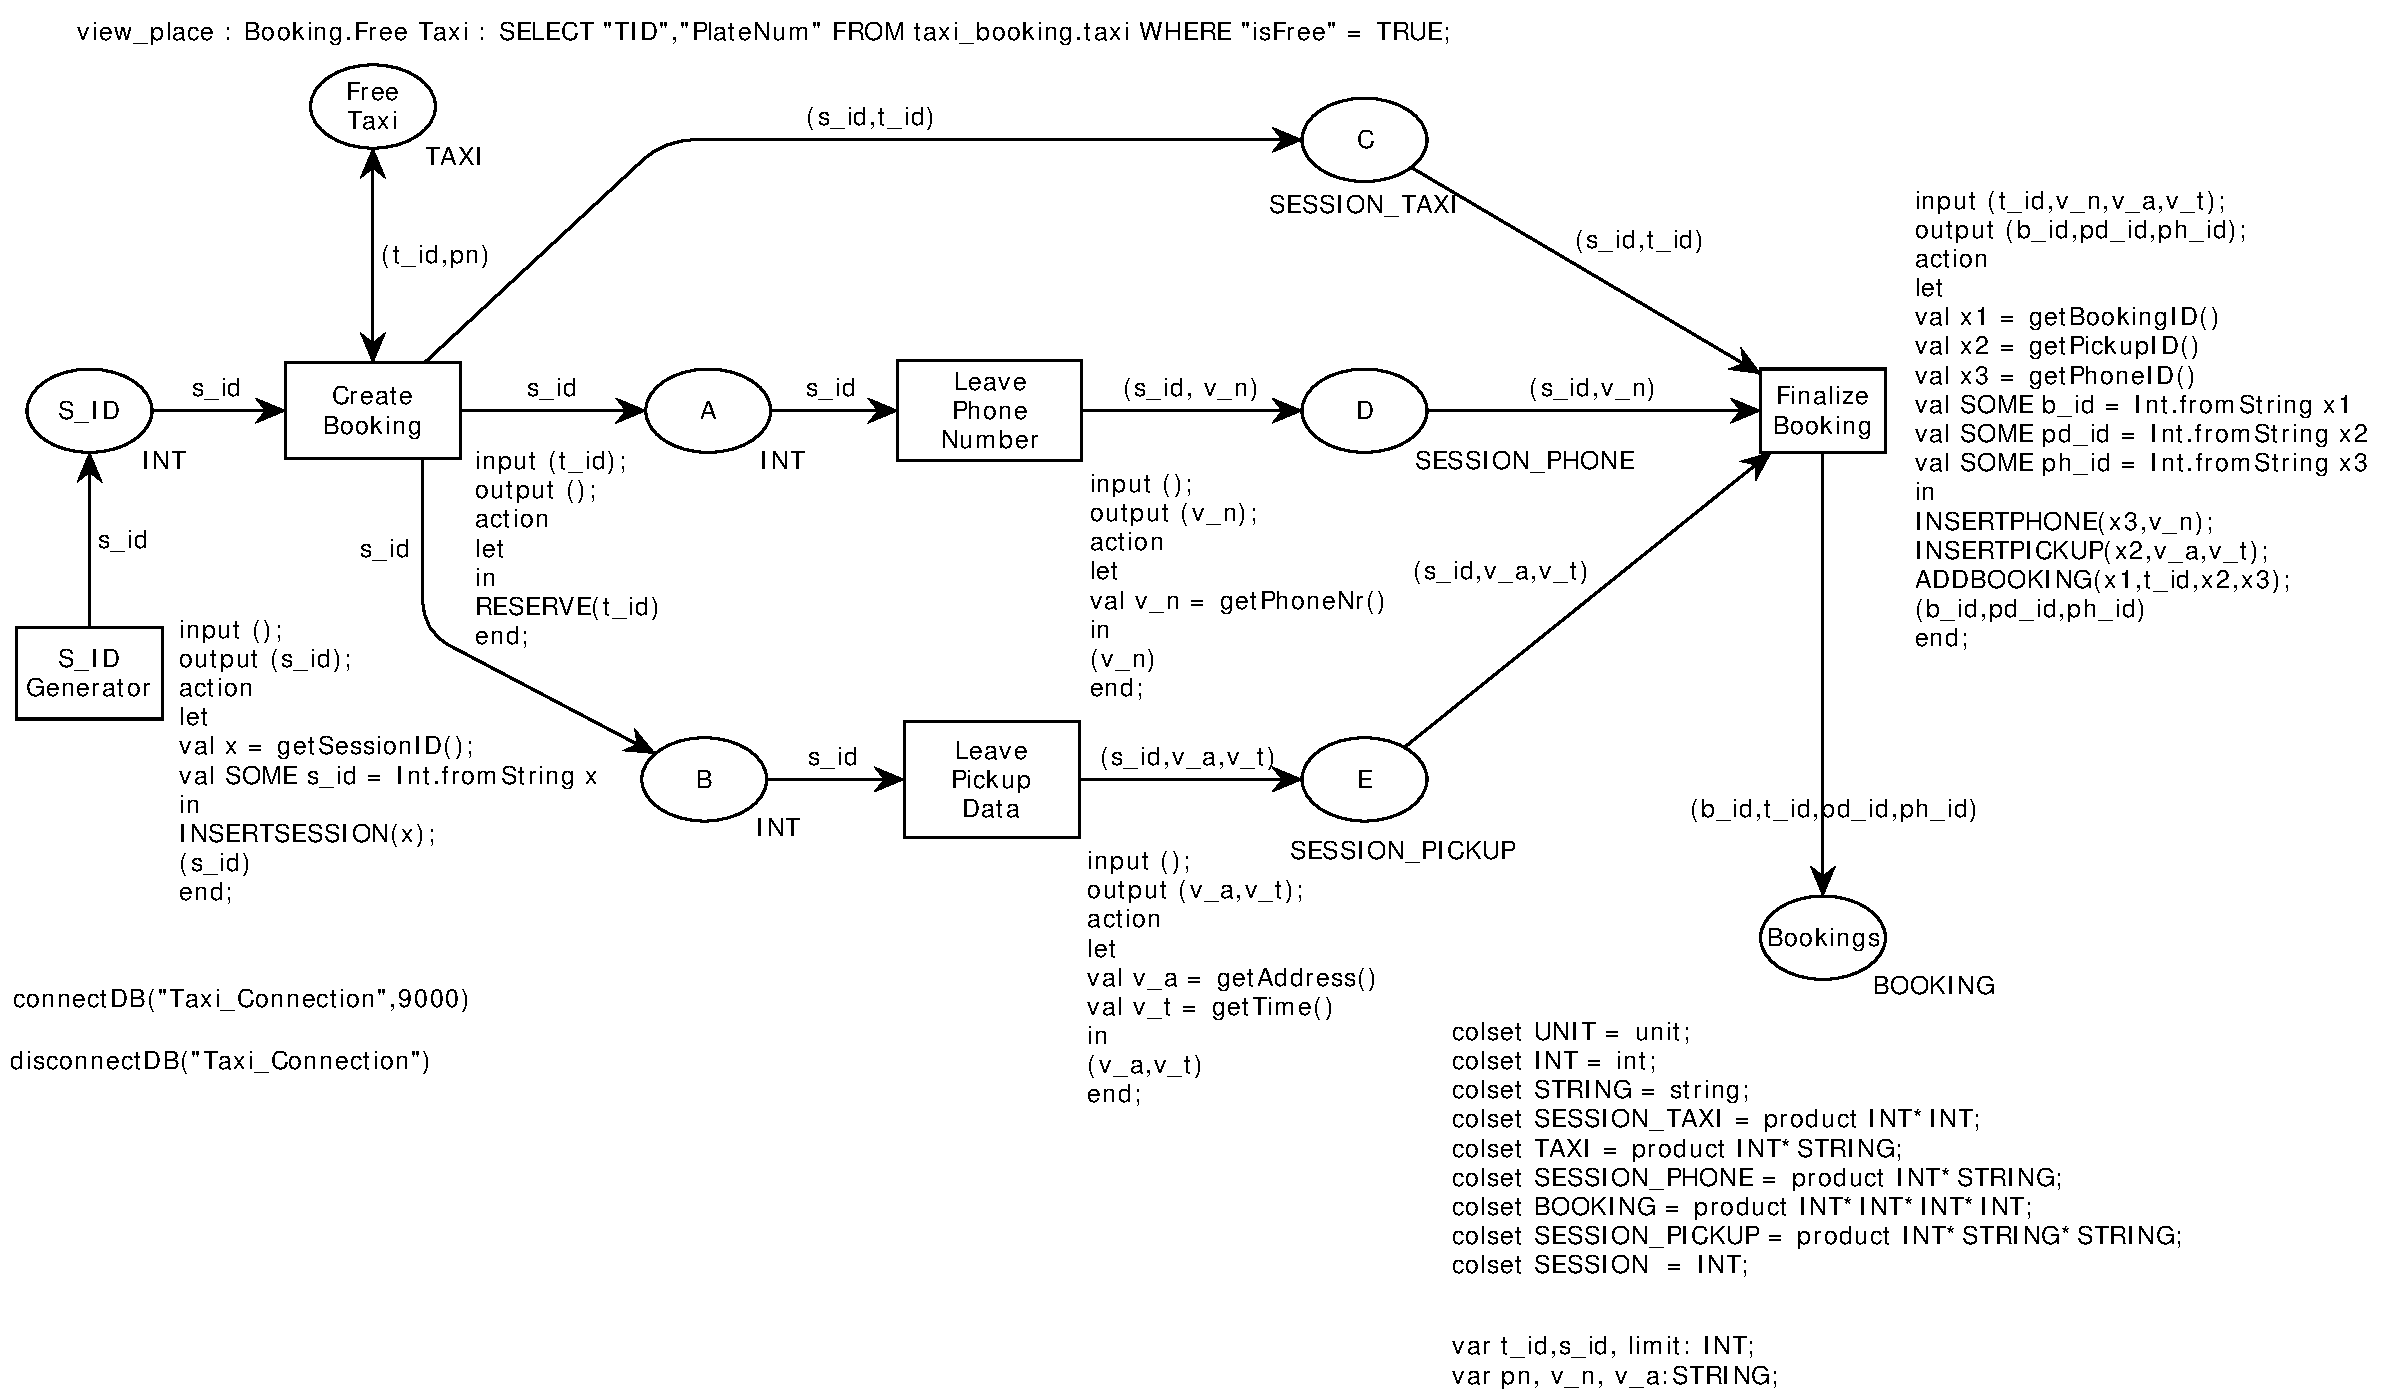
\includegraphics[scale = 0.35]{DBN_Impl_executable_model.pdf}
%	\caption{Executable DB-net model for taxi booking}
%	\label{fig:DBN_Impl_executable_model}
%\end{figure}
%
%\subparagraph*{\textnormal{In this model (see Figure \ref{fig:DBN_Impl_executable_model}), a session id generator (transition \textit{S\_ID Generator}) is attached which queries the \textit{session} table and generates an unique identifier for the table. The fresh variables generated by this transition is \textit{s\_id}. The \textit{action} part of \textit{S\_ID Generator} transition is: }}
%
%\subparagraph*{}
%\begin{lstlisting}[showstringspaces=false, language = ML, caption = Action part of transition : S\_ID Generator, captionpos=b, label = lst:DBN_Impl_action_sid_gen, numbers=left,
%stepnumber=1]
%let
%val x = getSessionID();
%val SOME s_id = Int.FromString x
%in
%INSERTSESSION(x);
%(s_id)
%end;
%\end{lstlisting}
%
%\subparagraph*{\textnormal{Functions \textit{getSessionID} and \textit{INSERTSESSION} are ML functions. \textit{getSessionID} generates a six digit unique session id for the \textit{session} table whereas \textit{INSERTSESSION} inserts the generated session id to the \textit{session} table. These ML functions can be defined as: }}
%
%\subparagraph*{}
%\begin{lstlisting}[showstringspaces=false, language = ML, caption = Functions for generating and inserting session ID, captionpos=b, label = lst:DBN_Impl_session_func,numbers=left,
%stepnumber=1]
%fun getSessionID() = getFromDB("taxi_booking.session","\"SID\"","genUniqueID","6");
%fun INSERTSESSION(s_id) = exQuery("exQuery","INSERT INTO taxi_booking.session VALUES ("^ s_id ^ ");" );
%\end{lstlisting}
%
%\subparagraph*{\textnormal{In Listing \ref{lst:DBN_Impl_action_sid_gen}, in line 2, variable \textit{x} stores the generated session ID from the \textit{getSessionID} function. In the DB-nets model the variable \textit{s\_id} is defined as \textit{integer}, hence we need to convert \textit{x} to \textit{integer}\footnote{The data type of the variable \textit{x} is \textit{string}, because it is returned from the function which uses Comms/CPN APIs which returns string.}. In line 6, the variable \textit{s\_id} is returned as the output variable.}}
%
%\subparagraph*{\textnormal{Let's take another example of the transition \textit{LEAVE PHONE NUMBER} where the data acquisition takes place without consulting the database. The \textit{action} part in this transition is defined as:}}
%
%\subparagraph*{}
%\begin{lstlisting}[showstringspaces=false, language = ML, caption = Action part of transition : LEAVE PHONE NUMBER, captionpos=b, label = lst:DBN_Impl_action_leave_ph_number, numbers=left,
%stepnumber=1]
%let
%val v_n = getPhoneNr()
%in
%(v_n)
%end;
%\end{lstlisting}
%
%\subparagraph*{\textnormal{In Listing \ref{lst:DBN_Impl_action_leave_ph_number}, the ML function \textit{getPhoneNr} internally calls \textit{getRandom} function which returns a randomly generated phone number of a fixed length. The ML definition of \textit{getPhoneNr} and \textit{getRandom} is:}}
%
%\subparagraph*{}
%\begin{lstlisting}[showstringspaces=false, language = ML, caption = Functions for acquiring phone number, captionpos=b, label = lst:DBN_Impl_getPhone_func]
%fun getPhoneNr()= getRandom("randomInt","10");
%\end{lstlisting}
%
%\subparagraph*{\textnormal{In Listing \ref{lst:DBN_Impl_action_leave_ph_number}, in line 2, the variable \textit{v\_n} acquires the ten digit phone number from the function \textit{getPhoneNr}. Similarly, for transition like \textit{Leave Pickup Data}, we could use different flavours of \textit{getRandom} function such as \textit{randomString} or \textit{randomTime}\footnote{for randomTime, one should always fix the length to 6, which signifies hh::mm::ss in the time format.}. The function for \textit{Leave Phone Number} transition is defined as follows:}}
%
%\subparagraph*{}
%\begin{lstlisting}[showstringspaces=false, language = ML, caption = Functions for acquiring address and time, captionpos=b, label = lst:DBN_Impl_add_time_func]
%fun getAddress() = getRandom("randomString","20");
%fun getTime() = getRandom("randomTime", "6");
%\end{lstlisting}
%
%
%\subparagraph*{\textnormal{Now we are aware about the modelling and execution of DB-nets in CPN Tools. If the reader is interested in more detailed and low level implementation of the extension, then one could read refer {\color{red}documentation link}. In the next chapter we will look at analysis on DB-nets.}}
%%\end{comment}


\graphicspath{{./images/DBN_SS/}}
\chapter{DB-nets Analysis : State Space}
\label{ch:DBN_SS}
\paragraph*{\textnormal{In the previous chapter, we discussed how to model DB-nets in CPN Tools. In this chapter, we try to generate state space for DB-nets using CPN Tools. In the attempt for generating state spaces, we mention our few failed attempts while constructing state space using CPN Tools. In the end, we present a workaround for calculating the state space.}}
\section{State Space}
\label{sec:DBN_SS_State_Space}
\paragraph*{\textnormal{State spaces in CPN Tools can be drawn with help of the state space tool\footnote{For information about using state space tool is explained in \cite{CPN_Tools_State_Space}.}. Here, we present a more abstract version of the taxi booking example in Figure \ref{fig:DBN_SS_Faulty_Net}. In this figure, we have intentionally kept our DB-net short in order to show the full state space.}}

\begin{figure}[!htbp]
	\centering
	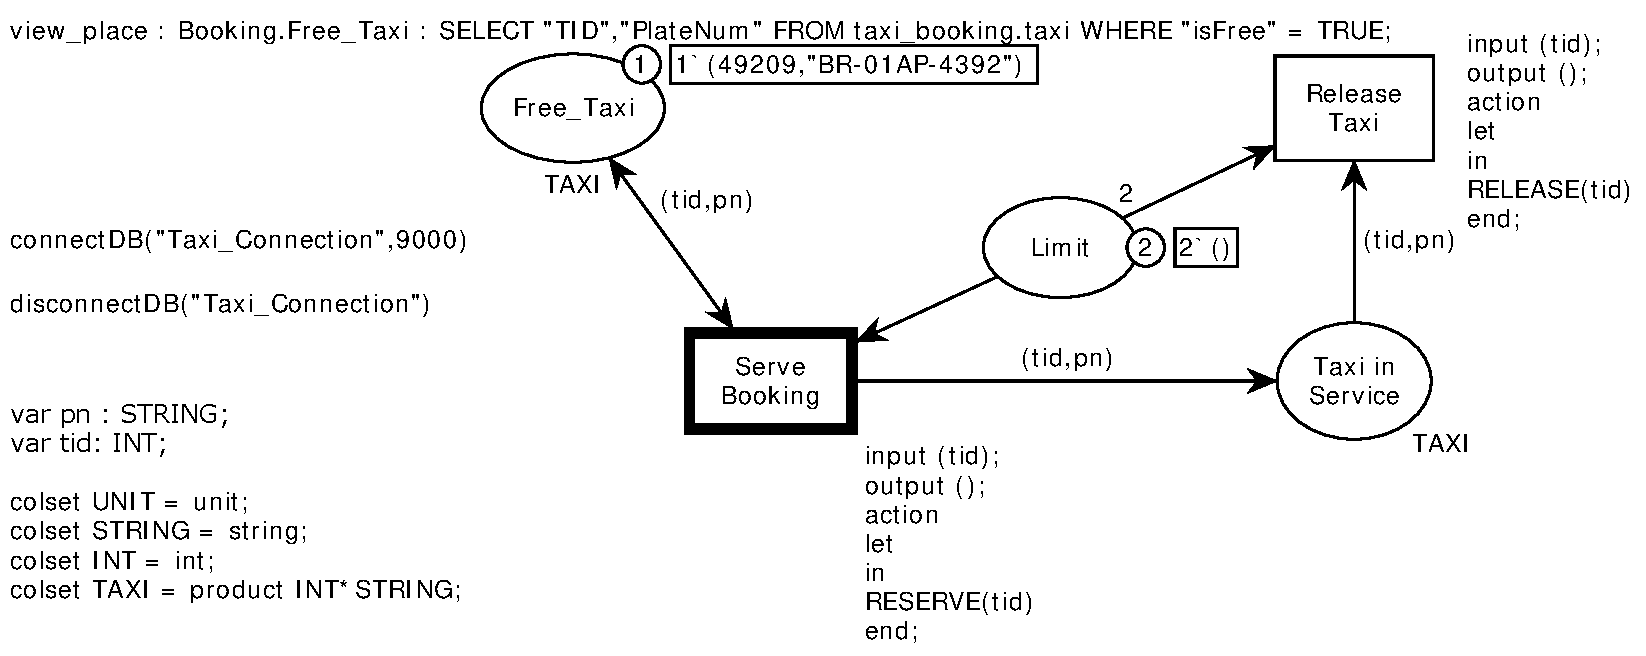
\includegraphics[scale = 0.40]{DBN_SS_Faulty_Net.pdf}
	\caption{Abstract net for taxi booking example}
	\label{fig:DBN_SS_Faulty_Net}
\end{figure}

\subparagraph*{\textnormal{In Figure \ref{fig:DBN_SS_Faulty_Net}, $\mathit{Free\_Taxi}$ is a view place(populated), $\mathit{Serve\ Booking}$ is an action transition which reserves a taxi, and makes it unavailable for further booking. Once the booking is served, the action transition $\mathit{Release\ Taxi}$ releases the taxi under service and makes it available for further booking. The place $\mathit{Limit}$ acts as the bound to the net by limiting the number of times the transitions can be fired. Here, we want to fire each transition only once. Figure \ref{fig:DBN_SS_Expected_SS} represents the expected\footnote{by \bsq{expected} we mean the ideal state space. Later we verify if we could obtain this state space using state space tool in CPN Tools.} state space for the DB-net model (Figure \ref{fig:DBN_SS_Faulty_Net}).}}

\begin{figure}[!htbp]
	\centering
	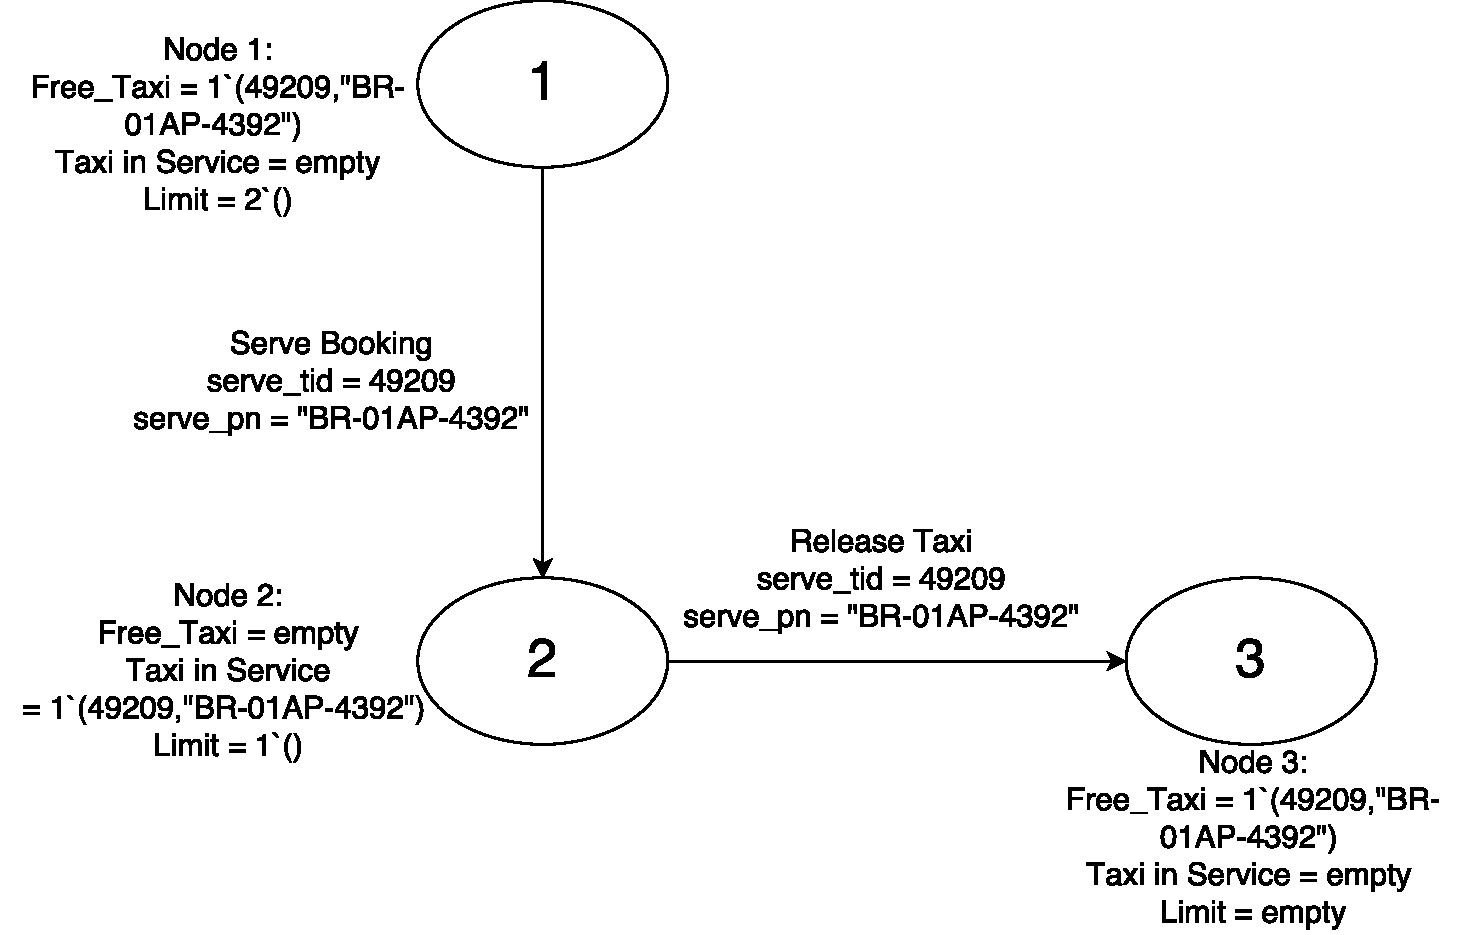
\includegraphics[scale = 0.40]{DBN_SS_Expected_State_Space.pdf}
	\caption{Expected state space for taxi booking example in Figure \ref{fig:DBN_SS_Faulty_Net}}
	\label{fig:DBN_SS_Expected_SS}
\end{figure}

\subparagraph*{\textnormal{However, when we analyse the DB-net (Figure \ref{fig:DBN_SS_Faulty_Net}) in CPN Tools, we receive the state space graph mentioned in Figure \ref{fig:DBN_SS_Faulty_Net_State_Space}. The uppermost integer in the node represents the node number whereas the numbers below it, in the format \[\langle numberofPredecessor : numberofSuccessor\rangle\] represents the number of predecessor and successor of the node. For example, node 1 has no predecessor and one successor. Similarly, node 2 has one predecessor (node 1) and two successors (node 3 and 4). The node markings are written beside the node and labels on the arcs are represented in the format \[\langle arcNumber : sourceNode \rightarrow targetNode\ transitionName : \{variableBindings\}\rangle\]For example, the directed arc between node 1 and 2 has the arc number 1, node 1 as the source node and node 2 as the target node. The transition fired is $\mathit{Booking\textquotesingle Serve\_Booking}$\footnote{It is the full qualified name of the transition, here $\mathit{Booking}$ is the page name in which the net is drawn and $\mathit{Serve\_Booking}$ is the transition name (spaces in the transition name are replaced with $\_$ symbol).} and the corresponding variable bindings are mentioned in the curly braces.}}

\subparagraph*{\textnormal{The reason for the incorrect state space calculated by CPN Tools is the inability to populate view places after firing transitions. Note that, the extension we developed is responsible for populating the view places. The state space tool in CPN Tools works as an extension and CPN Tools does not give us subscription to events occurring during state space generation\footnote{List of messages which could be subscribed by an extension are mentioned in \cite{CPN_Tools_Message_Format}.}. As a result, those events cannot be subscribed/listened by the extension and the view places are not populated.}}
\begin{figure}[!htbp]
	\centering
	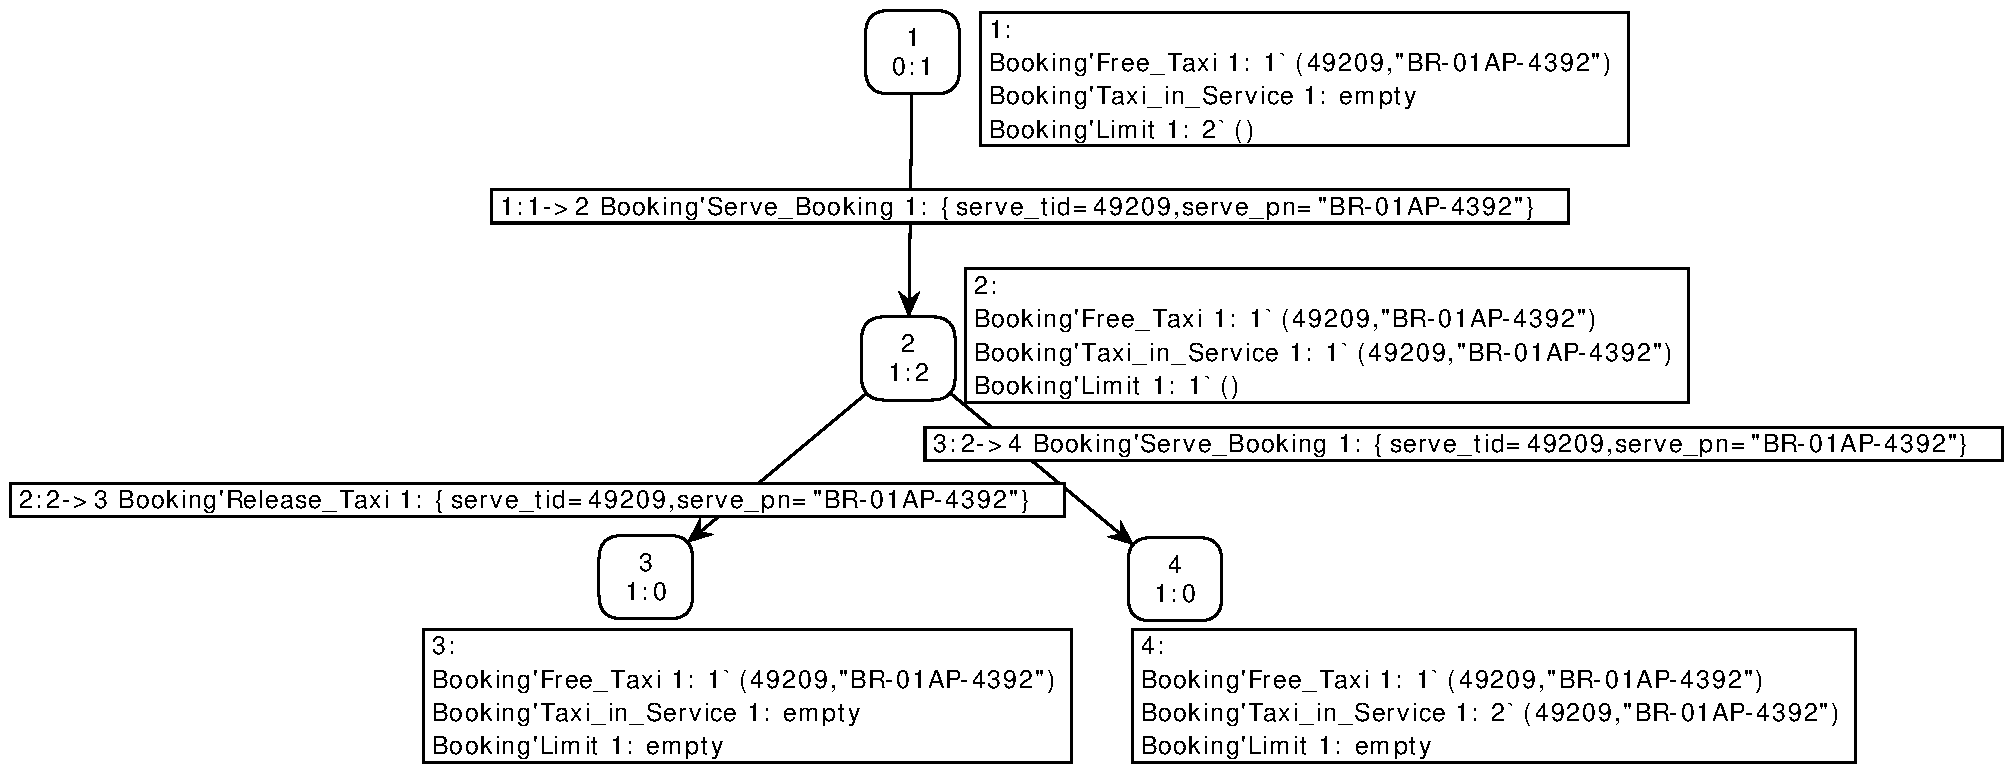
\includegraphics[scale = 0.40]{DBN_SS_Faulty_Net_State_Space.pdf}
	\caption{State Space calculated by CPN Tools for the net in Figure \ref{fig:DBN_SS_Faulty_Net}}
	\label{fig:DBN_SS_Faulty_Net_State_Space}
\end{figure}

\section{Failed Attempts}
\label{sec:DBN_SS_Failed_Attempts}
\paragraph*{\textnormal{We could successfully carry simulation over the DB-nets but we faced problem while analysing them. This section presents our failed attempts to perform analysis on DB-nets in CPN Tools. We mention our failed attempts as they are useful to understand state space generation in CPN Tools along with its relation with CPN Tools extension.}}

\subsection*{Intercepting state space construction events}
\paragraph*{\textnormal{As we mentioned earlier we could only subscribe to the events mentioned in \cite{CPN_Tools_Message_State_Space}. We tried to listen to the events which occur while drawing the state space diagram, e.g. show node marking, variable bindings of the arc etc. Once we receive the packet\footnote{The communication between GUI, simulator and extension is based on sending/receiving packets.}, we try to modify the packet by editing the node marking and replacing it with our desired marking. In the end, we return the modified packet. For example, we tried to modify the marking of node 2 (see Figure \ref{fig:DBN_SS_Faulty_Net_State_Space}) to our desired marking(by making the marking of the place $\mathit{Free\_Taxi}$ as empty). With this approach, the nodes can be modified with the desired marking, but properties such as total number of nodes (in state space), predecessor and successor needs to be changed. Even after changing the marking of the nodes, the state space report which provides the analysis of the net will yield undesired results. Intercepting state space construction events should be handled with utmost care because modifying the packet contents might lead CPN Tools into an inconsistent state, or in worst case can lead to a crash.}}

\subsection*{Shared architecture using Comms/CPN}
\paragraph*{\textnormal{We could observe that view places were not populated, but the actions in the transitions were properly executed. As mentioned, we could not capture the events, but using Comms/CPN, we could determine about the firing of the transition. We exposed a function $\mathit{refreshViewPlaces}$ from JAVA/CPN and this function was called at the end of the code segment of every transition. With this approach we created a shared architecture between the extension and JAVA/CPN as presented in Figure \ref{fig:DBN_SS_Layer_Architecture_Shared}.}}

\subparagraph*{\textnormal{In this attempt, we were successful in getting control from JAVA/CPN to the extension which was not possible in the earlier attempt. When the state space tool calculates the state space, it acquires the simulator lock and calculates its marking by firing transitions. The problem arose while updating the view place. In order to update the view place we acquire the simulator lock and send a request to GUI to update the view place. Since the simulator lock is already acquired by the state space tool, populating the view place ends up in a blocking queue where the extension waits indefinitely for the lock to get released. Since the extension is blocked, it cannot pass control to CPN Tools. Hence, we end up in an inconsistent state.}}

\begin{figure}[!htbp]
	\centering
	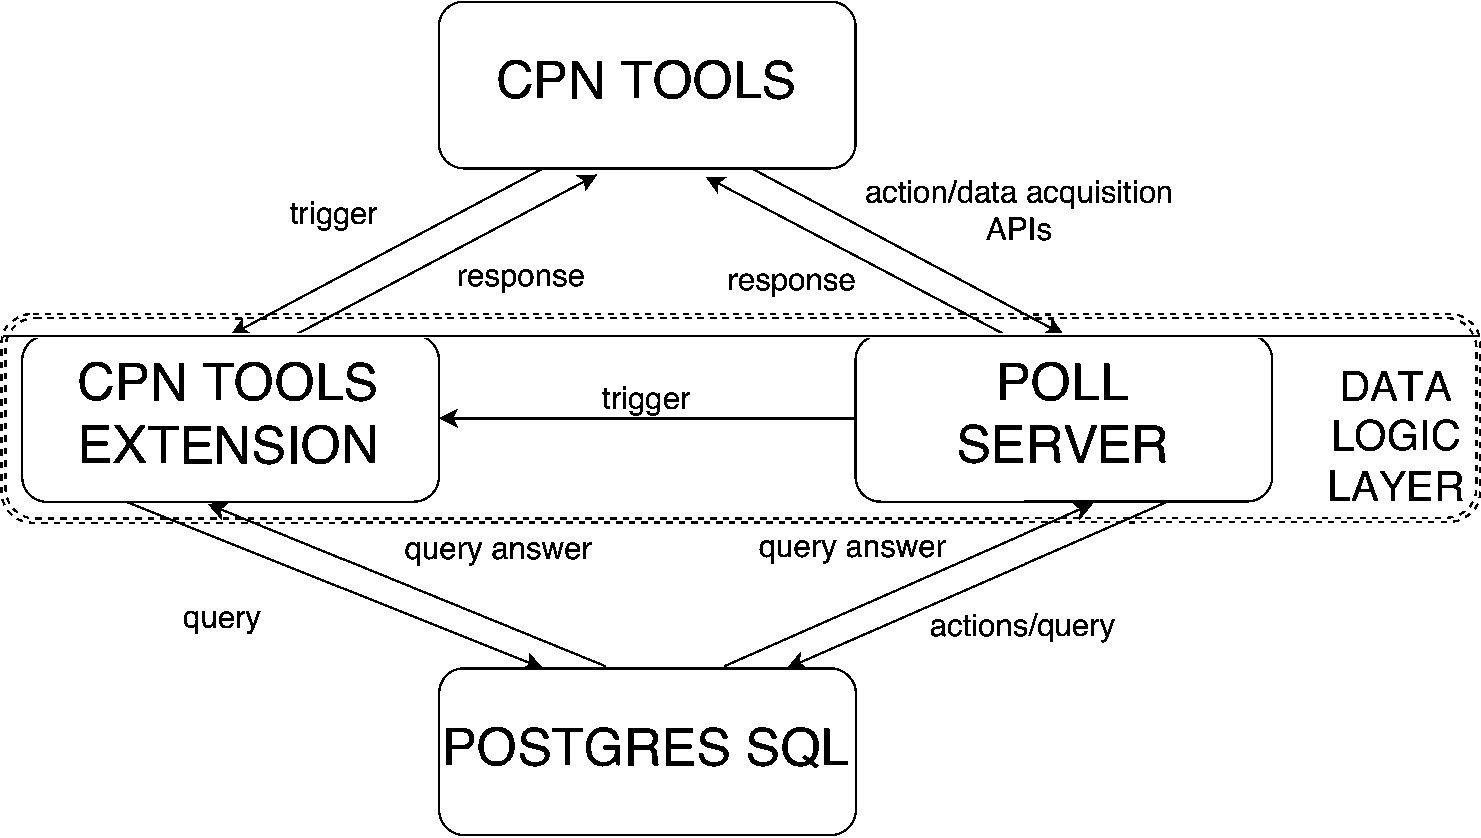
\includegraphics[scale = 0.40]{DBN_SS_Layer_Architecture_Shared.pdf}
	\caption{Shared architecture between extension and JAVA/CPN}
	\label{fig:DBN_SS_Layer_Architecture_Shared}
\end{figure}

\section{Compiling DB-nets into CPN}
\paragraph*{\textnormal{As stated earlier, the problem is to populate view places through the extension during state space calculation, hence we try to populate them through the net elements. Instead of relying on the database, we project the contents of the database on the control layer, and update the contents using net elements. In this approach, instead of view places we model \textit{relational places}. \textit{Relational places} are places which project the contents of the relational schema and the tokens in the relational places show the instances of the corresponding relational schema. The place colour mirrors the components of the relation schema and their types. In this light, each token represents a tuple in the database. Thus, with this approach we lift the database schema and model it in our control layer.  Later, we try to manually update the marking of the relational places by removing and/or inserting tokens corresponding to the actions attached to the transitions. In this workaround, the database is considered to be without any constraints. However, the proposed solution can seamlessly account for constraints as well.}}

\paragraph*{\textnormal{Before we introduce the modelling of relational places, we introduce \textit{priority} of a transition \cite{DBLP:conf/apn/WestergaardV11}. One can give high priority to a transition to force it to occur before all other enabled transitions, which can be used in case of exception handling by prioritizing the exception handler over other transitions handling usual cases. Similarly, one can assign lower priority to transition to prevent it from occurring unless no other transitions are enabled. As mentioned in \cite{CPN_Tools_Priority_Transitions}, in CPN Tools, we can assign priority to each transition. A \textit{priority} is simply a predefined integer\footnote{higher the value of integer, lower is the priority.} attached to a transition. If the priority of a transition is not explicitly defined, then it is considered as a \textit{NORMAL} priority transition. One can also define custom priorities in CPN Tools. In our case, we declare priority values as:
}}
\begin{verbatim}
val P_HIGH = 100;
val P_NORMAL = 1000;
val P_LOW = 10000;
\end{verbatim}}}

\subsection{View Place computation using Relational Places}
\label{subsec:DBN_SS_view_place_computation}

\subparagraph*{\textnormal{Let us consider a database schema \textit{organisation} containing the relational schema \textit{emp}, \textit{empDescr} and \textit{empID} as shown in Figure \ref{fig:DBN_SS_Relational_Schema}. The \textit{emp} table contains the id of the employee, name of the employee, and busy status of the employee. Table \textit{empDescr}\footnote{a short name for employee description.} contains the name of employees along with their designation and the table \textit{empID} contains the employee id. We use this database schema for modelling DB-net examples which are later transformed into CPNs.
\begin{figure}[!htbp]
	\centering
	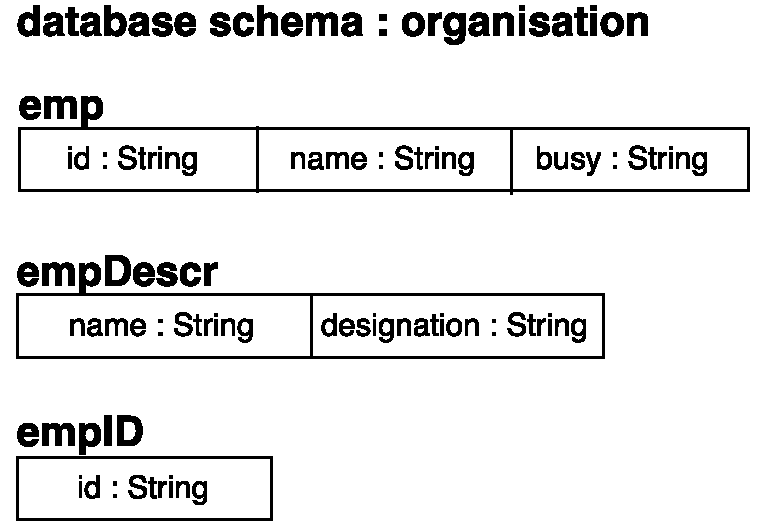
\includegraphics[scale = 0.50]{DBN_SS_Relational_Schema.pdf}
	\caption{Database Schema : organisation}
	\label{fig:DBN_SS_Relational_Schema}
\end{figure}
}}

\paragraph*{\textnormal{A small DB-net example is shown in Figure \ref{fig:DBN_SS_View_Place_1}, where we obtain a salary for a designation. The designation is computed using the \textit{View Place} and the query attached to it is:
\begin{figure}[h]
	\centering
	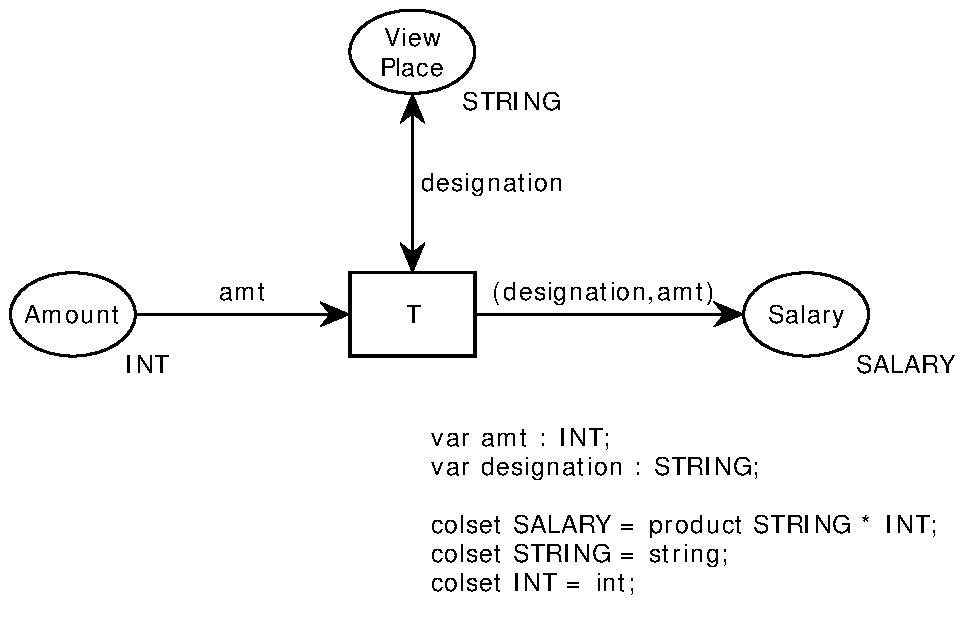
\includegraphics[scale = 0.50]{DBN_SS_View_Place_1.pdf}
	\caption{DB-nets: one view place}
	\label{fig:DBN_SS_View_Place_1}
\end{figure}}}

\subparagraph*{}
\begin{lstlisting}[showstringspaces=false, language = SQL]
SELECT organisation.empDescr.designation FROM organisation.empDescr, organisation.emp WHERE organisation.empDescr.name = organisation.emp.name;
\end{lstlisting}

\subparagraph*{\textnormal{Once	we have relational places, then we can compile away view places by reconstructing their content via a suitable query over relational places. Such a query can be formulated directly using arcs and inscriptions of the net, i.e., by resorting to standard elements in CPNs. Since, all queries attached to view places could not be evaluated using relational places, we restrict ourselves to conjunctive queries with filters. The filter condition in the conjunctive queries, attached to the view places, can be modelled using guards of the transition. For example, in Figure \ref{fig:DBN_SS_Relational_Place_1}, the relational places are modelled using places \textit{emp} and \textit{empDescr} projecting the contents of the corresponding relational schemas. The guard on the transition incorporates the filter condition.}}
\begin{figure}[h]
	\centering
	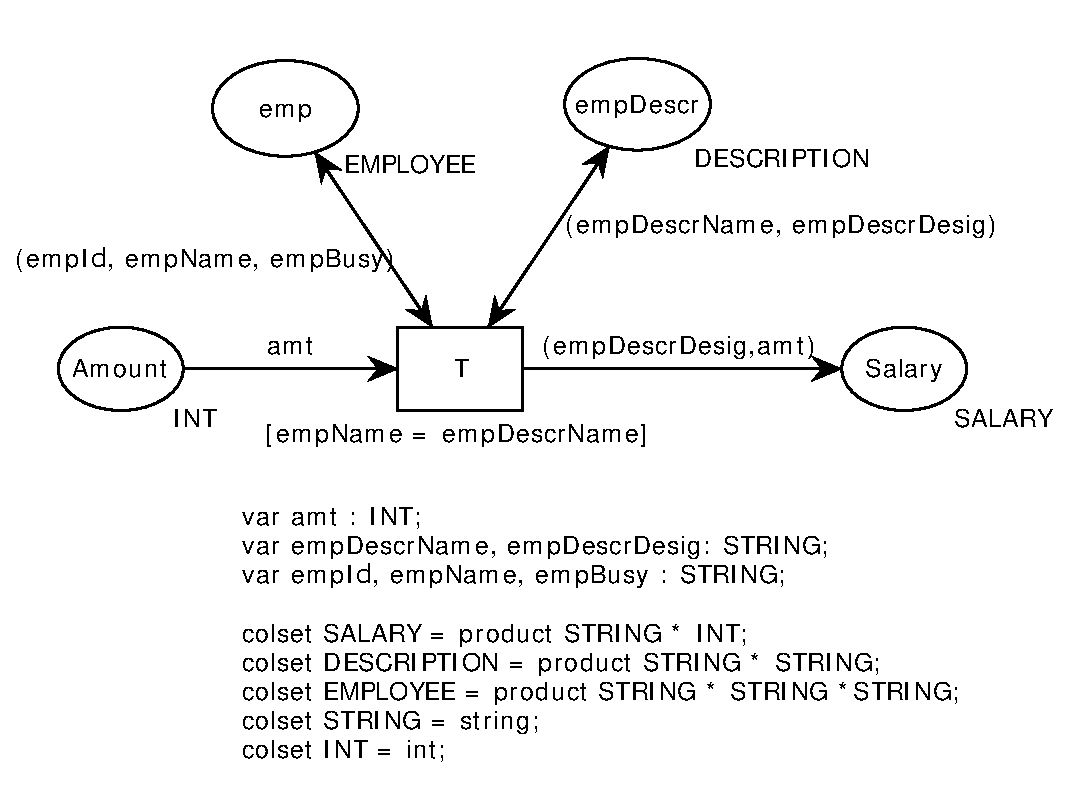
\includegraphics[scale = 0.50]{DBN_SS_Relational_Place_1.pdf}
	\caption{DB-nets: computing a view place using relational places}
	\label{fig:DBN_SS_Relational_Place_1}
\end{figure}

\subparagraph*{\textnormal{In case there are multiple view places sharing one or more relational schemas, the contents of the view place can be calculated in a sequential manner. Using a separate transition, we generate tokens of the first view place and then the generated tokens are forwarded to another transition which generates marking for the second view place. Similarly, in a serialized pipeline, one could calculate the result of two view places, and pass the result for calculation of third view place and so on. Let us consider an example of a transition connected to two view places as shown in Figure \ref{fig:DBN_SS_View_Place_2}. The query attached to the \textit{View Place 1} is same as the query attached to the \textit{View Place} in Figure \ref{fig:DBN_SS_View_Place_1}. The query attached to \textit{View Place 2} is:
\begin{figure}[!htbp]
	\centering
	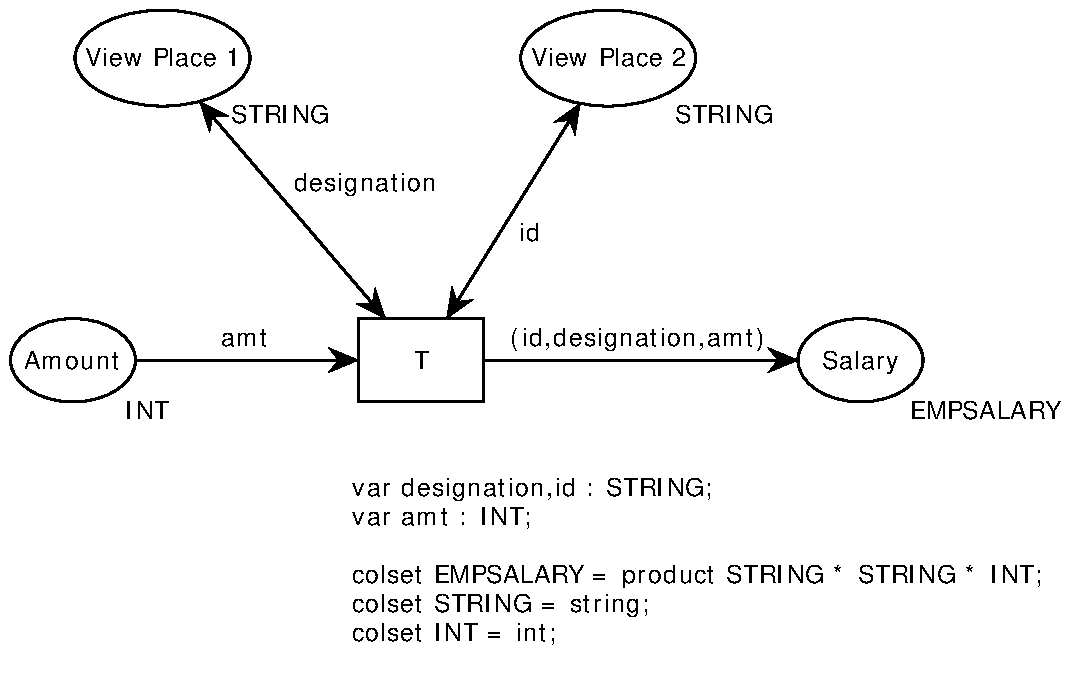
\includegraphics[scale = 0.50]{DBN_SS_View_Place_2.pdf}
	\caption{DB-nets: two view places}
	\label{fig:DBN_SS_View_Place_2}
\end{figure}
}}

\subparagraph*{}
\begin{lstlisting}[showstringspaces=false, language = SQL]
SELECT organisation.empID.id FROM organisation.empID, organisation.emp WHERE organisation.empID.id = organisation.emp.id;
\end{lstlisting}

\subparagraph*{\textnormal{The two view places use the common relational schema \textit{emp} to compute their markings. Using relational places, we could model the above net as shown in Figure \ref{fig:DBN_SS_Relational_Place_2}. In the figure, the transition \textit{Calculate View Place 1} acquires a lock (an uncoloured token) and generates a token for \textit{View Place 1} (see Figure \ref{fig:DBN_SS_View_Place_2}) which is stored at the place \textit{Result 1}. The transition $\mathit{T}$ has a higher priority (defined by the priority P\_HIGH) over the transition \textit{Release Lock}. If the transition \textit{T} is not enabled, then transition \textit{Release Lock} consumes the token from the place \textit{Result 1} and returns the lock. The purpose of lock is to allow the computation of each view place without any interruptions. Similarly, this sequential pipeline can be adopted if we have more than two view places which share a common relational schema.}}

\begin{figure}[!htbp]
	\centering
	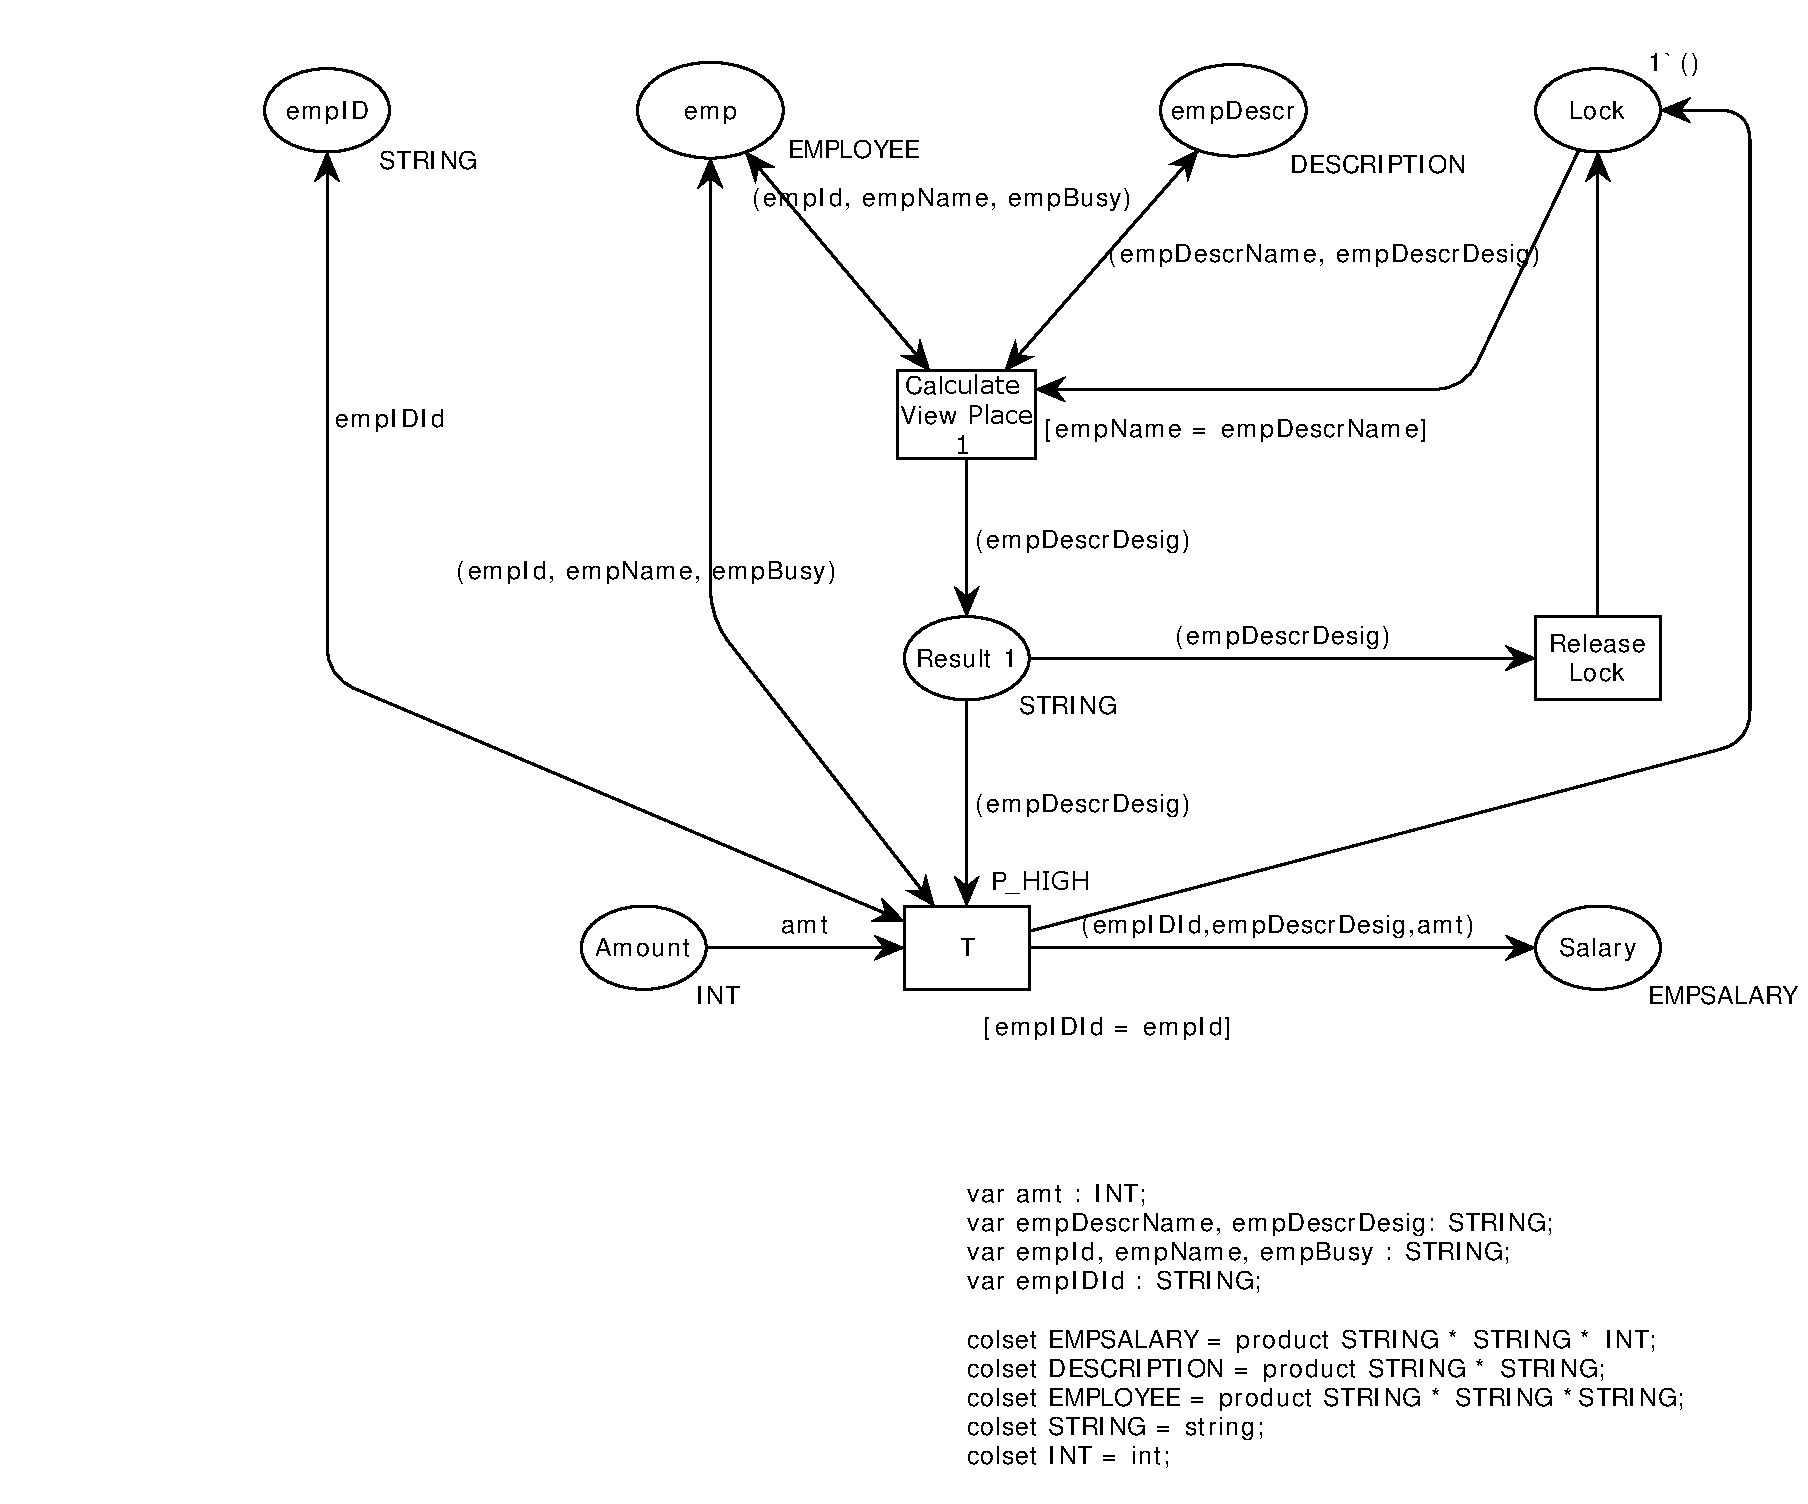
\includegraphics[scale = 0.40]{DBN_SS_Relational_Place_2.pdf}
	\caption{DB-nets: computing two view places using relational places}
	\label{fig:DBN_SS_Relational_Place_2}
	
\subparagraph*{\textnormal{Note that the $\mathit{READ}$ operation in DB-nets is modelled using view places. View places give us the partial information from the database instance whereas using relational places we represent the entire database instance. We can calculate the partial information (shown by view place) from the relational places and hence we do not need to explicitly model the read operation.}}
\end{figure}

\subsection{Transformation of Action Transitions}
\label{subsec:DBN_SS_Transformation_Action_Transitions}
\paragraph*{\textnormal{In the previous subsection, we discussed how to replace view places with relational places. In this subsection, we discuss about modelling the actions attached to a transition. In order to write into the database, we need to understand how to simulate actions over relational places. For further discussions, we use the DB-net modelled in Figure \ref{fig:DBN_SS_View_Place_1} and attach actions to the transition $\mathit{T}$.}}

\subparagraph*{\textnormal{As stated earlier, action transitions support addition and deletion of $\mathit{\mathcal{R}}$-facts, which should preserve the set semantics incorporated while modelling our persistence layer. In this workaround, the persistence layer is considered to be without any constraints. When we transform the operations, the action transition acquires the write lock before firing and releases the write lock when all the operations are executed. Figure \ref{fig:DBN_SS_Add_Operation} shows a DB-net with one transition that has an action attached which, in turn, adds a single entry to the $\mathit{empDescr}$ relational schema. In Figure \ref{fig:DBN_SS_Add_Operation_Relational_Place}, we model the net using relational places and reflect the effect of the add operation to the concerned relational place, i.e., $\mathit{empDescr}$.
\begin{figure}[!htbp]
	\centering
	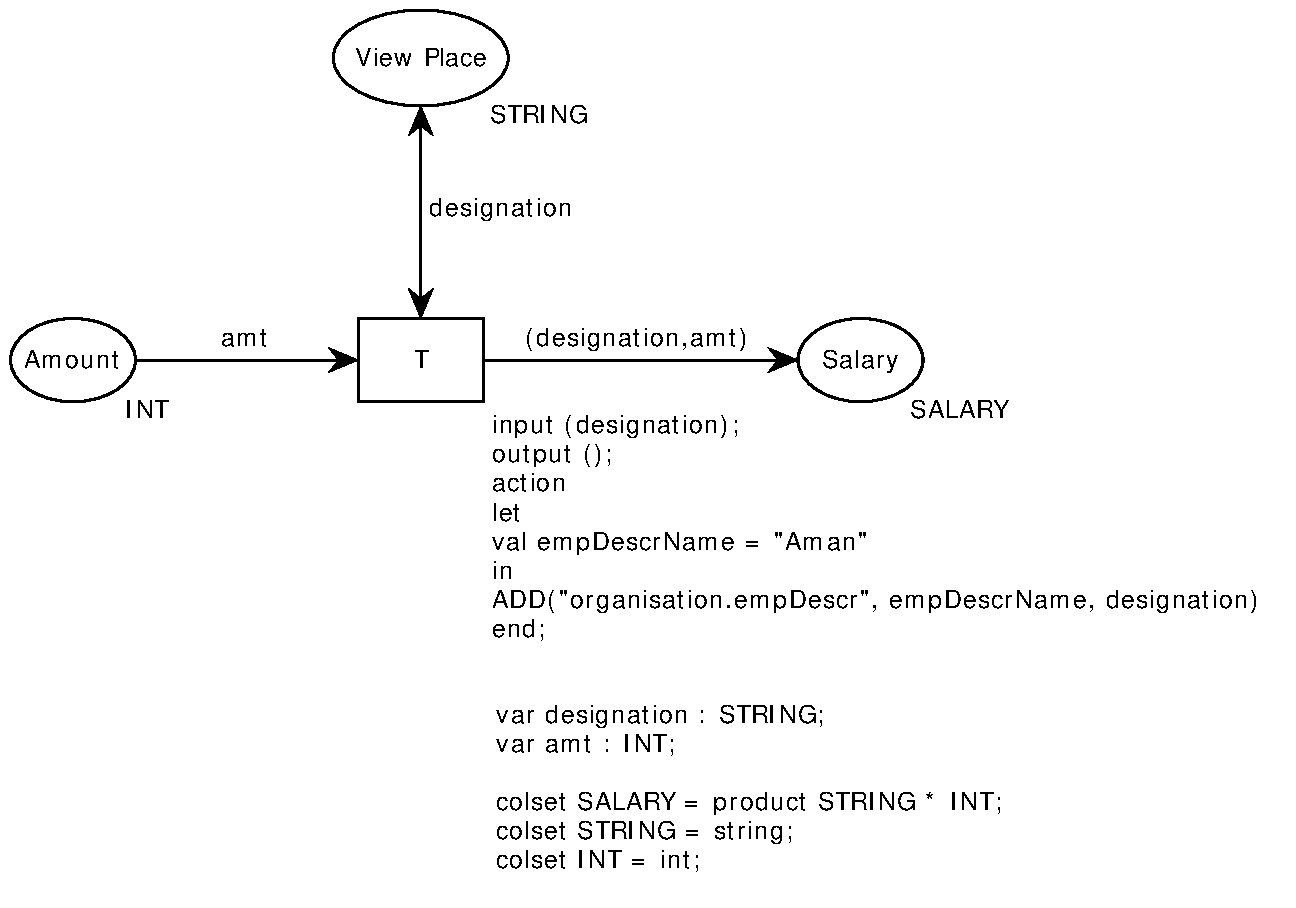
\includegraphics[scale = 0.40]{DBN_SS_Add_Operation.pdf}
	\caption{DB-nets: add operation}
	\label{fig:DBN_SS_Add_Operation}
\end{figure}
}}

\subparagraph*{\textnormal{In Figure \ref{fig:DBN_SS_Add_Operation_Relational_Place}, the transition $\mathit{T}$ acquires the \textit{write lock} (an uncoloured token) before firing. A \textit{write lock} is the lock which is acquired by an action transition to execute its action in a serialized manner. The tokens to be added are forwarded to the place $\mathit{toAdd}$. For preserving the set semantics over the relational place, with the help of priorities on the transitions, we first check if the entry already exists in the relational place. Note that the transition \bsq{$\mathit{exists\ in\ empDescr}$} has a higher priority than the transition \bsq{$\mathit{not\ exists\ in\ empDescr}$}. If the entry exists, then by firing \bsq{$\mathit{exists\ in\ empDescr}$} transition we do not add the token to the relational place, else we fire \bsq{$\mathit{not\ exists\ in\ empDescr}$} transition which adds a token to the relational place. After performing the add operation the write lock is returned.
\begin{figure}[!htbp]
	\centering
	\includegraphics[scale = 0.40]{DBN_SS_Add_Operation_Relational_Place.pdf}
	\caption{DB-nets: modelling add operation using relational places}
	\label{fig:DBN_SS_Add_Operation_Relational_Place}
\end{figure}
}}

\subparagraph*{\textnormal{Similarly, we can model the $\mathit{DELETE}$ operation. Let us consider the DB-net in Figure \ref{fig:DBN_SS_Delete_Operation}, where we perform a delete operation (attached to the transition $\mathit{T}$) on the relation schema \textit{empDescr}. The corresponding transformation of the DB-net is shown in Figure \ref{fig:DBN_SS_Delete_Operation_Relational_Place} where we reflect the delete operation in the relational place $\mathit{empDescr}$. Using priority between the transitions, we first check whether the token to be deleted exists in the relational place. If the token is present in the relational place, then we fire the transition $\mathit{exists\ in\ empDescr}$ and remove the token from the relational place, else we fire the transition \bsq{$\mathit{not\ exists\ in\ empDescr}$} and proceed.
\begin{figure}[!htbp]
	\centering
	\includegraphics[scale = 0.40]{DBN_SS_Delete_Operation.pdf}
	\caption{DB-nets: delete operation}
	\label{fig:DBN_SS_Delete_Operation}
\end{figure}
\begin{figure}[!htbp]
	\centering
	\includegraphics[scale = 0.40]{DBN_SS_Delete_Operation_Relational_Place.pdf}
	\caption{DB-nets: modelling delete operation using relational places}
	\label{fig:DBN_SS_Delete_Operation_Relational_Place}
\end{figure}
}}

\subparagraph*{\textnormal{For $\mathit{UPDATE}$ operation, we can model it using the transformation of DELETE and ADD operations. For update, we assume the case that when an update operation is performed, it should always preserve set semantics.}}

\begin{comment}
 For example, in Figure \ref{fig:DBN_SS_Update_Operation}, we perform an update operation on the relational schema $\mathit{empDescr}$ which updates the given designation to a new designation. The corresponding update operation can be modelled using relational places as shown in Figure \ref{fig:DBN_SS_Update_Operation_Relational_Place}. Here we assume that the tuple to be updated is already present in the relational place and after the update operation the set semantics is preserved at the relational place.}}
	
\begin{figure}[!htbp]
	\centering
	\includegraphics[scale = 0.40]{DBN_SS_Update_Operation.pdf}
	\caption{DB-nets: update operation}
	\label{fig:DBN_SS_Update_Operation}
\end{figure}

\begin{figure}[!htbp]
	\centering
	\includegraphics[scale = 0.40]{DBN_SS_Update_Operation_Relational_Place.pdf}
	\caption{DB-nets: modelling update operation using relational places}
	\label{fig:DBN_SS_Update_Operation_Relational_Place}
\end{figure}

\subparagraph*{\textnormal{Note that the $\mathit{READ}$ operation in DB-nets is modelled using view places. View places give us the partial information from the database instance whereas using relational places we represent the entire database instance. We can calculate the partial information (shown by view place) from the relational places and hence we do not need to explicitly model the read operation.}}
\end{comment}

\subparagraph*{\textnormal{In Figure \ref{fig:DBN_SS_Multi_Operations}, we have multiple operations defined in the action transition $\mathit{T}$. The order of execution of these operations are important and the \textit{delete} operation should be performed before the \textit{add} operation. While transforming the DB-net, we model these operations in sequential manner and after performing the last operation we finally return the write lock. The transformation of the DB-net (see Figure \ref{fig:DBN_SS_Multi_Operations}) is shown in Figure \ref{fig:DBN_SS_Multi_Operations_Relational_Places}. Delete operations are performed before add operations, so as to properly reconstruct the semantics of actions in DB-nets. Here, we sequentially perform delete and add operations and the intermediate result (after performing each operation) is propagated into the transformed net. For example, we first perform the delete operation, where we check if the entry exists in the relational place $\mathit{empDescr}$. If the corresponding entry exists in the relational place, then we delete the entry, else we simply propagate the intermediate result to the place $\mathit{toAdd}$. Similarly, for add operation, if the entry exists in the relational place, then we do not add the entry, else we add the entry and propagate the result to the place $\mathit{Salary}$. Since, the order of execution of \textit{delete} and \textit{add} operation is important, we serialize them in our net and return the write lock only when all the operations attached to the transition $\mathit{T}$ is carried out.}}

\begin{figure}[!htbp]
	\centering
	\includegraphics[scale = 0.40]{DBN_SS_Multi_Operations.pdf}
	\caption{DB-nets: action containing multiple operations}
	\label{fig:DBN_SS_Multi_Operations}
\end{figure}

\begin{sidewaysfigure}[!htbp]
\centering
\includegraphics[scale = 0.40]{DBN_SS_Multi_Operations_Relational_Places.pdf}
\caption{DB-nets: modelling all operations sequentially using relational places}
\label{fig:DBN_SS_Multi_Operations_Relational_Places}
\end{sidewaysfigure}

\subparagraph*{\textnormal{Let us incorporate the above mentioned modelling guidelines to model our taxi booking example shown in Figure \ref{fig:DBN_SS_Faulty_Net}. We model the net using relational places as shown in Figure \ref{fig:DBN_SS_Taxi_Booking_model}. Note that the relational place $\mathit{Taxi}$ is populated with three tokens where only the taxi with taxi id = 49209 is free. The guard of the transition $\mathit{Serve Booking}$ makes sure that only free taxi is read from the relational place. The state space calculated by the CPN Tools for this model is shown in Figure \ref{fig:DBN_SS_Correct_CPN_Tools}. Although, due to the presence the additional places and transitions the state space for this model has more nodes as compared the expected state space model (see Figure \ref{fig:DBN_SS_Expected_SS}), however the places of interest show correct markings.
\begin{figure}[!htbp]
	\centering
	\includegraphics[scale = 0.40]{DBN_SS_Taxi_Booking_model.pdf}
	\caption{Taxi Booking : Transformed net using relational places}
	\label{fig:DBN_SS_Taxi_Booking_model}
\end{figure}
}}

\subparagraph*{\textnormal{Notice that, due to the elimination of view places, the introduction of relational places, and the reconstruction of the semantics of actions via sequences of non-interruptible transitions, the resulting state space does not exactly correspond to the one induced by the original db-net. However, the two state spaces exactly correspond to each other when only focusing on control places and the reachability of their corresponding markings.}}

\begin{figure}[!htbp]
	\centering
	\includegraphics[scale = 0.40]{DBN_SS_Correct_CPN_Tools.pdf}
	\caption{Calculated state space for the model (in Figure \ref{fig:DBN_SS_Taxi_Booking_model}) using state space tool}
	\label{fig:DBN_SS_Correct_CPN_Tools}
\end{figure}




\chapter{Conclusion and Future Work}

\paragraph*{\textnormal{The idea of DB-nets was coined by Rivkin and Montali in their paper titled \bdq{DB-Nets: on The Marriage of Colored Petri Nets and Relational Databases}\cite{DBLP:journals/corr/DBNets}. In the paper, the authors emphasise on the theory behind different aspects of DB-nets and define it as an extension of Coloured Petri Nets. In this thesis, we implement the concept of DB-nets on the tools which are available for modelling, simulation and verification purposes. In this theory, we also present a lightweight theory related to the modelling of DB-nets in practice. However, in practice, we adopt the execution semantics similar to Coloured Petri Nets.}}

\subparagraph*{\textnormal{While calculating state spaces, we failed a few times and still do not have a clear solution for analysing DB-nets. We would like researchers to take up the task and look for a clean solution in future. In terms of practical application, one could also develop an extension which calculates the state space and export the results. In future, we could also help in setting benchmarks, by performing simulation over DB-nets, over which one could perform pattern recognition or process mining over them. We invite researchers to build up on this topic.}}
%\chapter{Producing the final version}
This chapter contains some suggestions that you may find useful 
when producing the final version of your dissertation.

\paragraph*{Page dimensions and font size.}
The FUB-CS Standard for printed dissertations is a
10 point font and a 240 mm x 170 mm size page (reduced B5 format).
The default for the FUB-CS Dissertation Style is a 12 point font and A4 paper.
This is so that you can enhance the appearance of your dissertation
by scaling down your camera-ready copy to 81\% of its original size.
If you have a high resolution printer, you may want to use a font size
of 10 or 11 points; 
the FUB-CS Dissertation Style determines the page dimensions of your dissertation 
depending on the the font size you choose, in such a way that the amount of
text on a page is the same.

\paragraph*{Posizioni - \emph{Stellungen}.}
Although you are not required to include a leaflet containing
Posizioni - \emph{Stellungen} with your dissertation, you may want to do that anyhow.
The following code is a way a producing such a leaflet.
\begin{verbatim}
  \documentstyle[12pt]{guide_diss}
  \begin{document}
  \begin{center}
  {\Huge Posizioni - \emph{Stellungen}}\\[4ex]
  dalla Tesi - \textit{zu den Doktorarbeit}\\[4ex]
  {\Large\em The FUB-CS Dissertation Style}\\[2ex]
  van\\[2ex]
  {\large John B. Goode}
  \end{center}
  \par\vspace {2.5\baselineskip}
  \begin{enumerate}
  \item This Stelling will get my name on national TV.
  \item And so will this one.
  \end{enumerate}
\end{verbatim}


\paragraph*{Saving paper.}
If anything, producing a dissertation costs a lot of paper.
When working on workstations you can save paper by previewing
rather than making printouts. At most sites you can also
save paper by using the command {\tt mpage -2 mydissertation.ps}
to print 2 pages of your dissertation on a single sheet of paper.
The \LaTeX{} command \verb|\includeonly{file1,file2,...}|
also allows you to save paper,
by allowing you to only print the parts of your document that have changed.
The file specified by an \verb|\include| command will only be processed if
it appears in the argument of the \verb|\includeonly| command.
If it doesn't appear, then it is omitted, but all succeeding text will be
processed as if the file had been inserted, numbering pages, sections,
equations etc. as if the omitted file's text had been inserted.
See also pp. 75-77 of the \LaTeX{} {\em User's Guide \& Reference Manual\/}.

\paragraph*{Font problems.}
A Latex installation usually includes a program called 
\verb|dvips| or \verb|dvi2ps|
which converts DVI-files generated by Latex to Postscript.
However, with the standard settings, the fonts contained
in the postscript file will be so-called `Type 3' (bitmapped) fonts, 
which are resolution-dependent. This may cause problems when you want 
to convert your document to PDF format or print it on printers with
very high resolutions (such as the printers at a professional printing
shop).
If you use the \verb|-Ppdf| flag, as in
\begin{verbatim}
  dvips -Ppdf myfile.dvi
\end{verbatim}
then the dvips program generates postscript files using
`Type 1' (scalable) fonts (provided these fonts are installed),
which should eliminate font problems.

If you want to create a PDF file from a Latex document, the easiest way is 
to use the dvips program to create a postscript file, and then convert
it into a PDF file using the \verb|ps2pdf| script (if installed). 
However, please note that
the \verb|ps2pdf| script uses the GhostScript program, and that versions
before Ghostscript 6.0 are \emph{not} capable of handling Type 1
LaTeX fonts. Instead, the fonts are converted them into Type 3 fonts, 
which (as stated above) can cause problems on printers with very high
resolutions. If your Ghostscript version is lower than 6.0
(you can check this by typing \verb|gs --version|),
and you cannot convince your System Administrator to update the
program, 
Adobe has an Online Conversion Service which offers free trials.
For more information on font problems, 
see the FUB-CS Support page on creating postscript files.


\appendix
\graphicspath{{./images/Appendix/Comparison_Tools/}}
\chapter{Comparison of Tools}
\label{ch:app_comp_tools}
\paragraph*{\textnormal{In order to develop an extension for extending CPN with relational database, we decided to choose a tool for our development. We discussed few potential candidate tools for the CPN extension. A database which lists all the available tools for PNs/CPNs is available at \cite{Tools_WIKI}. We wanted to develop the extension in a well known programming language such as Java, C, C++ etc. Potential tools such as Renew \cite{Renew_Paper} and CPN Tools, came up. CPN Tools is one of the most popular tool for modelling, simulating and verifying CPNs and is also used in industry\cite{CPN_Industrial_Use}. Kurt Jensen, first talked about CPN, in his paper \cite{Jensen2007} and also in his book \cite{Jensen_CPN_Book_ML} talks about modelling with CPN Tools. With the known popularity of CPN Tools, we decided to pick this tool for the development purpose along with Renew.}}

\begin{comment}
\paragraph*{\color {red}\textnormal{In this chapter, we will discuss about CPN Tools and Renew. The first part provides an introduction to Renew, whereas the second part gives an introduction of CPN Tools. Later, we compare the tool on few parameters and justify our selection of the tool for the development our extension. This chapter is intentionally made short. If the reader is interested in details, then one can follow the mentioned references.}}
\end{comment}

\section{Renew (The Reference NetWorkshop)}
\label{sec:app_comp_tools_renew}
\paragraph*{\textnormal{From \cite{Renew_Paper}, Renew is an extensible Petri net IDE that supports the development and execution of high-level Petri nets and other modelling techniques. One of the most attractive feature of Renew is implementation language, JAVA, which makes developing extensions easier (since it is one the well known programming language). The reference net formalism in Renew combines the concept of nets-within-nets with a reference semantics. Nets-within-nets simply builds a hierarchical structure of nets. Java being an object oriented language enhances its expressive power. Renew also has the support for Object-oriented PNs, Place/Transition Nets and Timed PNs.}}

\paragraph*{\textnormal{The first official release of Renew was in 1999. Since then TGI\footnote{Theoretical Foundations Group, Department of Informatics, University of Hamburg.} group has continuously developed it as a Petri net IDE. Renew allow modelling of Coloured Petri nets along with its simulation. Besides being a Petri net IDE, it also has plug-ins for other modelling techniques such as diagram from BPMN(Business Process Model Notation) or UML (Unified Modelling Language).}}
\subparagraph*{\textnormal{One of the main focus for the development of Renew is the simulation of reference nets. One of the approaches in software development with emphasis on distribution and concurrency is PAOSE\footnote{Petri Net-based agent-oriented software engineering \cite{DBLP:phd/de/Cabac2010}.}. In order to develop multi-agent applications (MAA), reference nets are used as implementation artifacts. So, in Renew we can also perform simulation, modelling, editing and debugging over a CPN model.}}

\subsection*{Modelling}

\subparagraph*{\textnormal{Figure \ref{fig:Comparison_Tools_Renew_Net_GCD} represents a CPN to find GCD (greatest common divisors) of numbers in Renew. The net contains 3 transitions, 2 places and 7 arcs. Places $P1$ and $P2$ are of type \textit{int}. The initial marking of $P1$ consists of 3 integers 105, 60 and 42. The variables in the arc expression are declared as integers (in the right most side of the figure). In Renew, the guards on transitions are defined with the prefix keyword \bdq{guard}(see transition \textit{T2}). The role of \textit{T1} is to eliminate a token of data value 0 from the place \textit{P1}. The role of the transition \textit{T2} is to take two integers from \textit{P1}, calculate their remainder and divisor and forward it to the place \textit{P2}. The transition \textit{T3} establishes a loop by transferring tokens from \textit{P2} to \textit{P1}. The process terminates when there is only one element left at place \textit{P1} and this is the resultant GCD of the tokens present at the initial state.}}

\subparagraph*{\textnormal{The net structure can be drawn with the tools provided in the tool box. For names, inscriptions and declaration of the net elements, separate tools are provided. The colour/type of the places can be declared by just writing the JAVA type beside the places.}}

\begin{figure}[!htbp]
	\centering
	\includegraphics[scale = 0.5]{Comparison_Tools_Renew_Net_GCD.pdf}
	\caption{CPN model to find the GCD of given numbers in Renew}
	\label{fig:Comparison_Tools_Renew_Net_GCD}
\end{figure}


\subsection*{Simulation}
\subparagraph*{\textnormal{Simulation in Renew is interactive. By interactive, we mean to say that the user can choose the enabled transitions to fire along with their bindings. During simulation, the marking of the places are displayed with no explicit feedback of the enabled transitions. However, double clicking on the transition will show if the transition is enabled and one could choose an enabled binding and fire the transition. The markings could also be seen by looking into the simulator log. The screen-shot of the net during simulation along with the simulation traces is given in Figure \ref{fig:Comparison_Tools_Renew_Sim_GCD}. The snapshot of the net is taken at the simulation step 5. In this state, there is a token at place \textit{P1} and 2 tokens at place \textit{P2}. The marking for each step is shown in simulation log. At this state the marking of the place \textit{P1} and \textit{P2} is given by:
\begin{equation*}
\begin{aligned}
m_{P1} =\ & 1^{\backprime}60\\
m_{P2} =\ & 1^{\backprime}3 +\!\!+ 1^{\backprime}42
\end{aligned}
\end{equation*}
Alternatively, one could also see the markings during simulation. The simulation comes to a halt when there are no more enabled transitions. Renew simulator also provides the user with the possibility to play a token game.}}
\begin{figure}[!htbp]
	\centering
	\includegraphics[scale = 0.7]{Comparison_Tools_Renew_Sim_GCD.pdf}
	\caption{Simulation Traces of CPN model in Figure \ref{fig:Comparison_Tools_Renew_Net_GCD}}
	\label{fig:Comparison_Tools_Renew_Sim_GCD}
\end{figure}
\begin{comment}
\subsection{Workflow}
\paragraph*{\textnormal{A short stepwise working of the net is mentioned below:
\begin{enumerate}
\item With the initial marking as 105, 60 and 42, transition $T1$ and $T3$ are disabled (since there are no tokens at place $P2$ and there is no token \bsq{0} at $P1$ for transition to have an enabled binding).
\item There is a non-deterministic choice available for variable $i$ and $j$. Let's suppose that variable $i$ has the binding of 60, in order to satisfy the guard of the transition $T2$, $i \geq j$, $j$ has to be 42. Now with the binding $i$ = 60 and $j$ = 42, $T2$ is fired and the result of $i\%j$ is 18 and the $P2$ has the marking as 18 and 42.
\item Anyone of the tokens present at $P2$ is then transfered to $P1$ (by firing $T3$) and the process is repeated until there are no more enabled transition.
\item When there are no more enabled transitions then the token at $P1$ is counted as the result.
\end{enumerate}}}
\end{comment}

\section{CPN Tools}
\label{sec:app_comp_tools_CPN_Tools}
\paragraph*{\textnormal{According to CPN Tools homepage \cite{CPN_Tools}, CPN Tools is a tool for editing, simulating and analysing Petri net. It was initially developed by the CPN Group at the Aarhus University, Denmark from 2000 to 2010. The main architects behind this tool are Kurt Jensen, S\o ren Christensen, Lars M. Kristensen, and Michael Westergaard. Now the tool has been transferred to the AIS group at Eindhoven University of Technology, The Netherlands.}}

\subparagraph*{\textnormal{CPN Tools has mainly two components namely the graphical editor and the back-end simulator. The graphical editor is written in BETA programming language where as the back-end simulator is written in CPN-ML \cite{CPN_Tools_Extension}. It also has the support for Timed PNs.}}

\subsection*{Modelling}
\subparagraph*{\textnormal{Figure \ref{fig:Comparison_Tools_CPN_Net_GCD} shows the net for calculating the GCD of numbers modelled in CPN Tools. The net structure is almost same as Renew, except the the colour-set definition. In CPN Tools, the colour-sets are defined using CPN-ML as contrary to JAVA syntax in CPN Tools. The work-flow of the net is exactly similar to the net shown in Figure \ref{fig:Comparison_Tools_Renew_Net_GCD}. To model the net, one can use the \textit{Create} palette from the tool box and select the tool under the palette. While selecting a graphical element and using the \bdsq{TAB} key (from the keyboard), one could set different properties for the GUI elements, e.g., guards for transitions, marking of a place, colour-set of a place etc. In CPN-ML one could write guards as the list of boolean expressions. The colour-sets and variables are declared in the declaration section as following:}}
\begin{figure}[!htbp]
	\centering
	\includegraphics[scale = 0.5]{Comparison_Tools_CPN_Net_GCD.pdf}
	\caption{CPN model to find the GCD of given numbers in CPN Tools}
	\label{fig:Comparison_Tools_CPN_Net_GCD}
\end{figure}
\subparagraph*{title}
\begin{lstlisting}[language = ML, caption = Colour set and variable declaration, captionpos=b, label = lst:colset_var_dec]
COLSET INT = int;
var i,j : INT;
\end{lstlisting}

\subsection*{Simulation}
\subparagraph*{\textnormal{CPN Tools simulator can be found in the \textit{Simulation} palette in the toolbox. There are many ways to simulate the model. One could play the token game an choose bindings manually. One could also limit the number of steps of simulation and allow the simulator to chose the binding non-deterministically. The simulation traces can also be exported as a report to a file. During simulation, the enabled transitions are highlighted \footnote{transitions represented by thick edges, see Figure \ref{fig:Comparison_Tools_CPN_Net_GCD}.}. The markings (during simulation) are represented by the rectangles beside the places.}}
\begin{figure}[!htbp]
	\centering
	\includegraphics[scale = 0.5]{Comparison_Tools_CPN_Sim_GCD.pdf}
	\caption{Simulation Traces of CPN model in Figure \ref{fig:Comparison_Tools_CPN_Net_GCD}}
	\label{fig:Comparison_Tools_CPN_Sim_GCD}
\end{figure}

\subsection*{Analysis}
\subparagraph*{\textnormal {Contrary to Renew, CPN Tools can also perform analysis on Coloured Petri nets. The tool provides the feature to calculate the state space of the net and analyse its behavioural properties such as liveliness, home markings etc. Analysis of the net is one of the crucial feature and this gives the tool an advantage to get incorporated in academic research and development. The state space graph \footnote{One could refer to the state space graph in section \ref{sec:CPN_Semantics}} for the model in Figure \ref{fig:Comparison_Tools_CPN_Net_GCD} is not shown because it is considerably large.}}

\section{Comparison}
\label{sec:app_comp_tools_comparison}
\paragraph*{\textnormal{We compare these two tools on different parameters and present a justification on the decision of the selection.}}

\subparagraph*{\textnormal{The documentation for Renew is available at \cite{Renew_Homepage} and for CPN Tools is available at \cite{CPN_Tools}. The source code for Renew is freely available at \cite{Renew_Homepage}, where as the source code for CPN Tools is not available. However, some modules of CPN Tools such as \textit{simulator} etc. can be downloaded. A comparison table is shown in the Table \ref{table:Comparison_Tools_Table}. We have considered few factors on which we evaluate both the tools.}}

\begin{table}[!tb]
	\centering
	\begin{tabular}{|c|c|c|}
		\hline
		Features                & Renew                  & CPN Tools       \\ \hline
		Implementation Language & JAVA                   & CPN-ML and BETA \\ \hline
		Platform Supported      & OSX, Windows, Linux 	 & Windows         \\ \hline
		Source Code             & Open Source            & Closed Source   \\ \hline
		Availability            & Free Available         & Free Available  \\ \hline
		Ease of Modelling       & Easy                   & Easy            \\ \hline
		Easy of Simulation      & Easy                   & Easy            \\ \hline
		Analysis                & Not Supported          & Supported       \\ \hline
		Debugger Support        & Yes                    & Yes             \\ \hline
		Extensibility           & Yes                    & Yes             \\ \hline
		Latest Version			& 2.5					 & 4.0.1			\\ \hline
	\end{tabular}
	\caption{Comparison Table}
	\label{table:Comparison_Tools_Table}
\end{table}

\subparagraph*{\textnormal{Renew gains advantage in most of the mentioned features. One such feature is its implementation language, JAVA, which is a very well known language in contrast to CPN-ML and BETA which is used by CPN Tools. Development in one of the well known programming language is easier. However, CPN Tools has exposed its APIs, through Access/CPN \cite{AccessCPN_Library}, in JAVA for developing extensions. Further, Renew is supported more known platforms such as Linux, OSX and even its experimental version of android exists. However, the major reason for our selection of CPN Tools over Renew is its wide use in industry along with its support for analysis of CP-nets.}}

\subparagraph*{\textnormal{For our purpose, we want to model non-hierarchical Coloured Petri nets and perform analysis of the net. Renew also supports modelling of non-hierarchical Coloured Petri nets but it does not support analysis. Renew can be a good contender in future for developing extensions once it starts supporting analysis over CP-nets.}}


%\chapter{Database Theory (Basics)}
\label{ch:db_basic}
\paragraph*{\textnormal{This chapter talks about the basic theory behind the database. We start with concepts in first order logic(FOL), and then we discuss first order logic queries followed by the discussion of translation of queries. For understanding the basic concepts of databases in this chapter, we refer \cite{DBLP:books/aw/found_DB}. \todo{citing diego slides?} Here we would discuss briefly about the FOL with equality which we will use in FOL queries.}}

\section{First Order Logic (FOL)}
\label{sec:db_theory_FOL}
\paragraph*{\textnormal{This logic can be used to represent the objects of the domain of discourse(the universe), about the properties of the objects and their relationships\footnote{properties corresponds to the unary predicate and the relations corresponds to \textit{n}-ary predicate}. Functions and Constants are also included in first order logic.}}

\subsection*{Syntax}
\subparagraph*{\textnormal{Variables $x_{1},x_{2},\ldots,x_{n}$ are called individual variables which denote single objects. The set of variables is denoted by:
\begin{equation*}
Vars = \{x_{1},x_{2},\ldots,x_{n}\}
\end{equation*}
A function symbol of arity $k$, where $k \geq 0$ and $x_{1},x_{2},\ldots,x_{k}$ are variables, is denoted as:
\begin{equation*}
f^{k}(x_{1},x_{2},\ldots,x_{k})
\end{equation*}
}}

\begin{defs}
The set of \textbf{Terms} is defined inductively as smallest possible set satisfying:
\begin{enumerate}
\item Each variable is a term . i.e. Vars $\subseteq$ Terms;
\item If $t_{1},t_{2},\ldots,t_{k} \in Terms$ and $f^{k}$ is a k-ary function symbol, then $f^k(t_{1},t_{2},\ldots,t_{k}) \in Terms$.
\end{enumerate}	 
\end{defs}

\begin{defs}
	The set of \textbf{Formulas} is defined inductively as smallest possible set satisfying:
	\begin{enumerate}
		\item If $t_{1},t_{2},\ldots,t_{k} \in Terms$ and $P^{k}$ is a k-ary predicate \footnote{a predicate of arity 0 is a proposition}, then $P^{k}(t_{1},t_{2},\ldots,t_{k}) \in$ Formulas(atomic formulas).
		\item If $t_{1},t_{2} \in Terms$, then $t_{1} = t_{2} \in Formulas$. (equality)
		\item If $\varphi \in Formulas$ and $\varphi \in Formulas$ then
		\begin{itemize}
			\item $\neg\varphi \in Formulas$
			\item $\varphi \wedge \psi \in Formulas $
			\item $\varphi \wedge \psi \in Formulas $
			\item $\varphi \rightarrow \psi \in Formulas$
		\end{itemize}
		\item If $\varphi \in Formulas$ and $x \in Vars$ then
		\begin{itemize}
			\item $\exists x.\varphi \in Formulas$
			\item $\forall x.\varphi \in Formulas$
		\end{itemize} 
	\end{enumerate}	 
\end{defs}

\subsection*{Semantics}
\paragraph*{\textnormal{Following the FOL syntax, we will have a look at the semantics of the language.}}
\begin{defs}
	Given an \textbf{alphabet} of predicates $P_{1},P_{2},\dots$ and function symbols $f_{1},f_{2},\ldots$ each with an associated arity, a FOL \textbf{interpretation} is:
	\begin{equation*}
		I = (\Delta^{I},\cdot^{I})
	\end{equation*}
where:
\begin{itemize}
	\item $\Delta^{I}$ is the interpretation domain (a non-empty set of objects);
	\item $\cdot^{I}$ is the interpretation function that interprets predicates and function symbols as:
	\begin{itemize}
		\item if $P_{i}$ is a k-ary predicate, then $P_{i}^{I} \subseteq \Delta^{I} \times \ldots \times \Delta^{I}$ (k times)
		\item if $f_{i}$ is a k-ary function, $k \geq 1$, then $f_{i}^{I} : \Delta^{I} \times \ldots \times \Delta^{I} \rightarrow \Delta^{I}$
		\item if $f_{i}$ is a constant, then $f_{i}^{I} : () \rightarrow \Delta^{I}$, which means $f_{i}$ denotes exactly one object in the domain.
	\end{itemize} 
\end{itemize}
\end{defs}

\begin{defs}
	Given an interpretation I, an \textbf{assignment} is a function
	\begin{equation*}
		\alpha : Vars \rightarrow \Delta^{I}
	\end{equation*}
that assigns to each variable $x \in Vars$ an object $\alpha(x) \in \Delta^{I}$. We could extend the notion of assignments to terms. We define a function $\hat{\alpha} : Terms \rightarrow \Delta^{I}$ inductively as follows:
\begin{itemize}
	\item $\hat{\alpha}(x) = \alpha (x)$, if $x \in Vars$
	\item $\hat{\alpha}(f(t_{1},\ldots,t_{k})) = f^{I}(\hat{\alpha}(t_{1}),\ldots,\hat{\alpha}(t_{k}))$
	\item for constants $\hat{\alpha}(c) = c^{I}$
\end{itemize}
\end{defs}

\subparagraph*{\textnormal{We define a FOL formula $\varphi$ is true in a interpretation $I$ with respect to an assignment $\alpha$, written $I,\alpha \models \varphi$:}}
\begin{equation*}
\begin{cases}
I,\alpha \models \varphi & if $(\hat{\alpha}(t_{1}),\ldots,\hat{\alpha}(t_{k})) \in P^{I}$\\
I,\alpha \models t_{1} = t_{2} &  if $\hat{\alpha}(t_{1}) = \hat{\alpha}(t_{2})$\\
I,\alpha \models \neg \varphi & if $I,\alpha \nvDash \varphi$ \\
I,\alpha \models \varphi \wedge \psi & if $I,\alpha \models \varphi$ and $I,\alpha \models \psi$\\
I,\alpha \models \varphi \vee \psi & if $I,\alpha \models \varphi$ or $I,\alpha \models \psi$\\
I,\alpha \models \varphi \rightarrow \psi & if $I,\alpha \models \varphi$ implies $I,\alpha \models \psi$\\
I,\alpha \models \exists x .\varphi & if for some $a \in \Delta^{I}$ we have $I,\alpha\lbrack x \mapsto a \rbrack \models \varphi$\\
I,\alpha \models \forall x .\varphi & if for every $a \in \Delta^{I}$ we have $I,\alpha\lbrack x \mapsto a \rbrack \models \varphi$
\end{cases}
\end{equation*}

\subparagraph*{\textnormal{where $\alpha\lbrack x \mapsto a \rbrack$ stands for the new assignment obtained from $\alpha$ as follows:}}
\begin{equation*}
\begin{aligned}
\alpha\lbrack x \mapsto a \rbrack(x) &= a \\
\alpha\lbrack x \mapsto a \rbrack(y) &= \alpha (y),\hspace*{1 cm} \textnormal{for }y \neq x
\end{aligned}
\end{equation*}

\subsection*{Relational Schema and Database Schema}
\subparagraph*{\textnormal{Inspired from \cite{DBLP:books/aw/found_DB}, we assume \textit{domain} as a countably infinite set $\Delta$, \textit{attributes} as a finite set \textit{U}, and a mapping function $dom:U\rightarrow\Delta$ and $dom(A)$ is called domain of $A$, where $A \in U$.}}

\begin{defs}
	\label{defs:dbn_sort_function}
	A function \textit{sort} is defined as $sort:R^{n}\rightarrow{\mathcal{P}^{fin}}(U)$, where ${\mathcal{P}^{fin}}$ is the finitary powerset\footnote{the set of finite subsets} of attributes, $R^{n}$ is the set of relation schema and $U$ is the finite set of attributes.
\end{defs}

\subparagraph*{\textnormal{The sort of a relation schema \textit{R} is simply written as \textit{sort(R)} and the arity is written as $arity(R) = |\textit{sort(R)}|$. A relational schema (\textit{R}) and set of attributes(\textit{U}) together make up the structure of the table. $R[U]$ is used to represent $sort(R) = U$, and $R[n]$ to represent $arity(R) = n$.}}

\begin{defs}
	\label{defs:dbn_database_schema}
	For a given domain $\Delta$, a \textbf{database schema} is a non empty finite set $\mathcal{R}$ of relational schemas, written as:
	\begin{equation*}
	\mathcal{R} = \{R_{1}[U_{1}],\ldots,R_{n}[U_{n}]\}
	\end{equation*}
	where $R_{1},\ldots,R_{n}$ are relational schemas and $U_{1},\ldots,U_{n}$ are attributes
\end{defs}

\subsection*{First order logic queries}
\begin{defs}
A first order logic \textbf{query} is an (open) FOL formula. Let $\varphi$ be a first order logic query with free variables $(x_{1},\ldots,x_{k})$, the query is written as:
\begin{equation*}
\varphi (x_{1},\ldots,x_{k})
\end{equation*}
and we say that the query has arity k.
\end{defs}
\paragraph*{\textnormal{For a given interpretation $I$, the only interesting assignments are those which map the variables $x_{1},\ldots,x_{k}$. We write an assignment $\alpha$ such that $\alpha(x_{i}) = a_{i},$ for $i = 1,\ldots,k$ as $\langle a_{1},\ldots,a_{k} \rangle$.}}

\begin{defs}
Given an interpretation $I$, the \textbf{answer to a query} $\varphi (x_{1},\ldots,x_{k})$ is :
\begin{equation*}
{\varphi (x_{1},\ldots,x_{k})}^{I} = \{(a_{1},\ldots,a_{k}) | I,\langle a_{1},\ldots,a_{k} \rangle \models \varphi (x_{1},\ldots,x_{k}) \}
\end{equation*}
\end{defs}

\subparagraph*{\textnormal{Notation $\varphi ^ I$ is used which keeps the free variables implicit, and $\varphi(I)$ is used for making apparent that $\varphi$ becomes a function from interpretations to set of tuples.}}

\begin{defs}
A \textbf{first order logic boolean query} is a first order logic query without free variables.
\end{defs}

\subparagraph*{\textnormal{The answer to the boolean query is defined as:
\begin{equation*}
{\varphi()}^{I} = \{() | I,\langle \rangle \models \varphi() \}
\end{equation*}
such an answer is :
\begin{itemize}
\item \bdq{true}, the empty tuple (), if $I \models \varphi$
\item \bdq{false}, the empty set $\emptyset$, if $I \nvDash \varphi$
\end{itemize}}}

\subsection*{\color{red} Translation of queries needs to be written.}

\subparagraph*{\textnormal{A \textit{\textbf{multiset} m} over a non-empty set $S$ can be thought as a function which maps an element $s \in S$ to a natural number in $\mathbb{N}$ which denotes the number of appearances of the element $s$. The natural number $m(s)$ is also called coefficient of $s$ in $m$. We use ${}^{\backprime}$ as the infix operator. The number preceding the symbol ${}^{\backprime}$ signifies the coefficient of $s$ in $m$ while the tuple succeeding the symbol represents the element.
}}
\subparagraph*{\textnormal{Let us formally define multisets:}}
\begin{defs}
	\label{defs:Multiset}
	Let $S = \{ s_{1}, s_{2}, s_{3}, . . . \}$ be a non-empty set. A \textbf{multiset} over S is
	a function $m : S \rightarrow \mathbb{N}$ that maps each element $s \in S$ into a non-negative integer $m(s) \in \mathbb{N}$ called the \textbf{number of appearances} (coefficient) of $s, where s \in S$, in $m$. A multiset $m$ can also be written as a sum:
	\begin{equation*}
	_{}^{++}\sum\limits_{s \in S}^{ } {m(s)}^{\backprime}s = {m(s_{1})}^{\backprime} s_{1} +\!\!+ \ {m(s_{2})}^{\backprime}s_{2} +\!\!+ \ {m(s_{3})}^{\backprime} s_{3} +\!\!+ \ldots
	\end{equation*}
	\textbf{Membership, addition, scalar multiplication, comparison,} and \textbf{size} are defined
	as follows, where $m_{1}, m_{2}$, and m are multisets, and $n \in \mathbb{N}$ :
	\begin{enumerate}
		\item $\forall s \in S$ : $s \in m \Leftrightarrow  m(s) > 0$. (Membership)
		\item $\forall s \in S$ : $(m_{1}$ $+\!+$ $m_{2})(s)$ = $m_{1}(s) + m_{2}(s)$. (Addition)
		\item $\forall s \in S : (n$ $\ast\!\ast$ $m)(s) = n$ $\ast$ $m(s)$. (Scalar multiplication)
		\item $m_{1}$ $\ll=$ $m_{2}$ $\Leftrightarrow \forall s \in S : m_{1}(s) \leq m_{2}(s)$. (Comparison)
		\item $\left | m \right | = \sum\limits_{s \in S} m(s)$. (Size)
		\item A multiset m is \textbf{infinite} if $\left | m \right | = \infty$. Otherwise m is \textbf{finite}. When $m_{1} \ll= m_{2}$, \textbf{subtraction} is defined as:
		\begin{center}
			$\forall s \in S$ : $(m_{2}$ $--$ $m_{1})(s) = m_{2}(s) - m{1}(s).$
		\end{center}
	\end{enumerate}
	The set of all multisets over S, i.e., the multiset type over S is denoted $S_{MS}$. The
	empty multiset over S is denoted by $\emptyset_{MS}$ and is defined by $\emptyset_{MS}(s) = 0$ for all $s \in S$.
\end{defs}
\subparagraph*{\textnormal{This covers the basic definition of multisets and some of their operations namely addition, scalar multiplication, subtraction, size etc. In this definition there are new symbols defined for addition ($+\!+$), scalar multiplication ($\ast\!\ast$), comparison ($\ll=$) and subtraction ($--$). In further discussions, we would use these notations.}}



%%  \include the `end matter'
\bibliographystyle{IEEEtran}
\bibliography{guide_bib_file.bib}


%%  finally, \include the list of previous FUB-CS dissertations

\cleardoublepage % if you are so inclined
%\pagestyle{empty}

\noindent
\begin{center}
\textbf{Titles in the FUB-CS Dissertation Series}\\
Collana di Tesi\\
{\em Reihe von Doktorarbeiten}
\par\vspace {1cm}
\end{center}

\newcommand{\fubcspublication}[3]{\item[FUB-CS #1: ]{\bf #2}\\{\em #3}}

\begin{list}{}{ \settowidth{\leftmargin}{ILL}
		\setlength{\rightmargin}{0in}
		\setlength{\labelwidth}{\leftmargin}
		\setlength{\labelsep}{0in}
}

\fubcspublication{DS-2008-01}{Catharina Maria Keet}{A Formal Theory of Granularity}
\fubcspublication{DS-2008-02}{Bruno Rossi}{Towards a Simulation Model including Network Externalities in Free/Libre Open Source Software (FLOSS) Adoption}
\fubcspublication{DS-2008-03}{Dino Seppi}{Prosody in Automatic Speech Processing}

\end{list}

\clearpage
\mbox{ }
\newpage

 %PERSONALIZE that is: make sure you have the latest list.
%{\pagestyle{empty}
\normalsize
\setlength\columnsep{20pt}
%      \columnseprule \z@
 %  \columnsep 35\p@
\par\vskip 1cm
%\begin{backsummary} %add later, see also fubdiss2.cls
   \twocolumn[{\Large FUB CS Diss Style}\\  %%PERSONALIZE
\textsl{any subtitle goes here}\vspace{8mm}] 		%PERSONALIZE

your summary of about 1 column goes\\
your summary of about 1 column goes here\\
your summary of about 1 column goes here\\
your summary of about 1 column goes here\\
your summary of about 1 column goes here\\
your summary of about 1 column goes here\\
your summary of about 1 column goes here\\
your summary of about 1 column goes here\\
your summary of about 1 column goes here\\
your summary of about 1 column goes here\\
your summary of about 1 column goes here\\
your summary of about 1 column goes here\\
your summary of about 1 column goes here\\
your summary of about 1 column goes here\\
your summary of about 1 column goes here\\
your summary of about 1 column goes here\\
your summary of about 1 column goes here\\
your summary of about 1 column goes here\\
your summary of about 1 column goes here\\
your summary of about 1 column goes here\\
your summary of about 1 column goes here\\
your summary of about 1 column goes here\\
your summary of about 1 column goes here\\
your summary of about 1 column goes here\\
your summary of about 1 column goes here\\
your summary of about 1 column goes here\\
your summary of about 1 column goes here\\
your summary of about 1 column goes here\\
your summary of about 1 column goes here\\
your summary of about 1 column goes here\\
your summary of about 1 column goes here\\
your summary of about 1 column goes here\\
your summary of about 1 column goes here\\
your summary of about 1 column goes here\\
your summary of about 1 column goes here\\
your summary of about 1 column goes here\\
your summary of about 1 column goes here\\
your summary of about 1 column goes here\\
your summary of about 1 column goes here\\
your summary of about 1 column goes here\\
your summary of about 1 column goes here\\
your summary of about 1 column goes here\\
your summary of about 1 column goes here\\
your summary of about 1 column goes here\\
your summary of about 1 column goes here\\
and balance it out a bit so that the logo is somewhere in the middle. alternatively, there is a 
\begin{verbatim}
\begin{backsummary} 
your summary goes here. 
see also fubdiss2.cls
\end{backsummary}
\end{verbatim}
%\end{backsummary}
\begin{center}
%\par\vspace {2cm}
\par\vspace {3.5cm}
\noindent%
\fublogo{7cm}
\end{center}
\vfill

%Copyright and accreditation stuff, plus ISBN
%
\noindent%
%\fubcslogo{5cm}\\
% Copyright: put your name here
\hfill Copyright \copyright\ 200x by John B. Goode\\[1ex] %PERSONALIZE
% Cover design, if your cover was designed by someone else
%Cover design by Mickey Mouse.\\                       %PERSONALIZE
%Maybe some additional info on the production of the dissertation.
%Don't forget your printing shop
\noindent \mbox{ } \hfill Printed and bound by DigiPrint\\[2ex]           %PERSONALIZE
%ISBN number: ask your faculty library how to obtain one
%\noindent \mbox{ } \hfill ISBN: 90--XXXX--XXX--X                              %PERSONALIZE
} 

%%%%%%%%%%%%%%%%%%%%%%%END of BACK MATTER%%%%%%%%%%%%%%%%%%%%%%%%%%%
 % for a thesis with a back-flap summary
%% This is the standard `front matter' to be used with the illcdiss.cls
%% Latex2e document class or the illc_diss.sty Latex2.09 style file
%%
%% Author: Maarten de Rijke
%% Current maintainer: Marco Vervoort
%%
%% Version: July, 2001
%%
%% MAKE SURE THAT THE FILE HAS BEEN PERSONALIZED BEFORE YOU
%% PRINT AND SHIP THE FINAL VERSION.  YOU CAN FIND ITEMS THAT NEED
%% TO BE PERSONALIZED BY SEARCHING FOR THE STRING ``%PERSONALIZE''
%%
%%
%%first of all the cover.
{\pagestyle{empty}
%\newcommand{\printtitle}{%
%{\Huge\bf The FUB-CS Dissertation\\[0.8cm] Style}}    %PERSONALIZE

%%the second page: the `illc pagina'
\clearpage
\par\vskip 2cm
\begin{center}
\par\vspace {2cm}
%\textbf{FUB-CS Dissertation Series DS-200X-NN}                 %PERSONALIZE
%\par\vspace {1cm}
%\noindent%
\fublogo{14cm}
\end{center}

\vfill

%Copyright and accreditation stuff, plus ISBN
%
\noindent%
%\fubcslogo{5cm}\\
% Copyright: put your name here
Copyright \copyright\ 2017 by Aman Sinha\\[2ex] %PERSONALIZE
% Cover design, if your cover was designed by someone else
%Cover design by ------.\\                       %PERSONALIZE
%Maybe some additional info on the production of the dissertation.
%Don't forget your printing shop
Printed and bound by your printer.\\[2ex]           %PERSONALIZE
%ISBN number: ask your faculty library how to obtain one
ISBN: 90--XXXX--XXX--X                              %PERSONALIZE

% Dedication, table of contents and acknowledgements
% are handled in the main file

\clearpage
} % Back to \pagestyle{plain}

%%%%%%%%%%%%%%%%%%%%%%%END of BACK MATTER%%%%%%%%%%%%%%%%%%%%%%%%%%%
 %or take this one for a fairly plain back cover
 
\end{document}